%\part{Anhang}

\chapter*{Katalog A: Grabungsbefunde (Kat.-Nr.~1--19)}\label{sec:BefBeschr}
\addcontentsline{toc}{chapter}{Katalog A: Grabungsbefunde (Kat.-Nr.~1--19)}
\chaptermark{Katalog A: Grabungsbefunde (Kat.-Nr.~1--19)}
\sectionmark{Katalog A: Grabungsbefunde (Kat.-Nr.~1--19)}
%\subsection*{Vorbemerkungen}
\begin{multicols}{2}
\raggedcolumns
\noindent Der Katalog beschreibt die im Zuge dieser Arbeit untersuchten Grabungsbefunde (Teil~A) und Inventare aus Oberflächenabsammlungen (Teil~B) aus Kampagnen des \textit{River Reconnaissance Project} von 1985 und 1987. Alle Angaben beruhen auf den Aufzeichnungen der Ausgräber.

Die Ordnung beider Katalogteile folgt der Fundplatz-Nummerierung (Abb.~\ref{fig:ArbeitsgebietKarte} und Anlage 1.B). Daraus ergibt sich, dass Einträge entlang der Flüsse \mbox{Ubangi}, \mbox{Lua}, \mbox{Kongo}, \mbox{Sangha}, \mbox{Ngoko} und \mbox{Likwala}-\mbox{aux}-\mbox{Herbes} entgegen der Fließrichtung gereiht sind. 

Die Aufarbeitung der in Katalog A untersuchten Grabungsbefunde richtete sich nach dem Umfang der Maßnahme und der angewandten Grabungstechnik. Die Gliederung der einzelnen Katalogeinträge folgt jedoch einem einheitlichen Schema. Von diesem wurde nur in Einzelfällen abgewichen, entweder weil die entsprechenden Informationen nicht verfügbar waren oder zusätzliche Quellengattungen zu diskutieren waren. Nach der Beschreibung der Grabung und der freigelegten Befundlage erfolgt eine Ansprache der keramischen Fundinventare sowie sonstiger Funde. Der Datierungsansatz und eine knappe Interpretation bilden den Abschluss eines jeden Eintrages.

Künstliche Grabungseinheiten sind systematisch als \textit{Abträge} bezeichnet und sind von natürlichen Schichten und beobachteten Befunden (Gruben, Verfüllungsbereiche etc.) zu unterscheiden. Wo möglich, wurde letztere detailliert beschrieben und in eingeklammerten Zahlen markiert. Tiefenangaben beziehen sich, wo eine Umrechnung möglich war, auf die Tiefen unter Oberfläche, wie sie sich aus der Umrechnung der im Gelände, basierend auf einen vor der Grabung vermarkten Nivellierpunkt, dokumentierten Messprotokolle ergab. Die Färbung der Sedimente und Verfüllungen folgt der Notation der \textsc{Munsell Soil Color Charts}.

Das für die Auswertung der keramischen Inventare zugrunde gelegte Aufnahmeschema ist in Kap.~\ref{sec:GefKeramik} erläutert. Bereits im Feld ausgesondertes Material wurde, soweit dies die Dokumentation zuließ, in die Auswertung einbezogen. Für die in den grafischen Darstellungen zur Verteilung keramischer Stile genutzten Abkürzungen siehe Anlage 3. Die Färbung der Stilgruppen in den Verteilungsdiagrammen folgt den Übersichtsdarstellungen in den Abb.~\ref{fig:EIA1}--\ref{fig:LIA3}. Die Verteilungen der \textit{Fabrics} orientiert sich an Abb.~\ref{fig:Fabrics_Verbreitung}.

Die zeichnerische Umsetzung der Plana und Profile erfolgte unter Umrechnung der im Feld dokumentierten \textsc{Munsell}-Farben in RGB-Werte, die anschließend in Graustufen übertragen wurden. Die entsprechenden Zeichnungen wurden zudem so weit zusammengeführt und vereinheitlicht, dass sich eine kohärente Darstellung der Befundlage ergab. Schichtnummerierungen sind durchweg in einem Kreis verzeichnet, während die Nummerierung von Gefäßen oder Gefäßeinheiten in einem Quadrat erfolgte.

In Katalog B sind alle in dieser Arbeit untersuchten Inventare aus Surveys zusammenfassend und in Listenform beschrieben. Die Auflistung erfolgt separiert nach den chronologisch sortierten Stilgruppen\footnote{Siehe Anlage 3 für die genutzten Abkürzungen.} sowie nach Gefäßen (Gef.), Rand- (RS), Wand- (WD) und Bodenscherben (BS). Surveys wurden, wenn möglich, auf allen vegetationsfreien Flächen durchgeführt, um möglichst repräsentative Fundinventare für jeden Platz zu erhalten. Dabei erfolgte häufig eine Trennung nach topografischen Kriterien, vor allem zwischen den Uferbereichen und freien Dorfflächen.%\columnbreak 
\end{multicols}
\newpage
\begin{multicols}{2}
\raggedcolumns
\section*{\begin{tabular*}{\linewidth}{@{}l @{\extracolsep{\fill}} r@{}}
Nr.~1 & MLB~85/1-3-1 \\
\end{tabular*} 
}

\textsf{\textbf{Maluba (Lua; Fpl.~230)}}

\vspace{1em}

\noindent\begin{tabular}{@{}rl@{}}
\textbf{Feldarbeit:} & \begin{tabular}[t]{@{}l@{}}\textbf{05.09.--08.09.1985}\\ \textbf{(M. K. H. Eggert/F. Nikulka)}\end{tabular} \\ 
\textbf{Abb.:} & \textbf{\ref{fig:MLB85_1_Zeichnung}--\ref{fig:MLB85_1_14C-Kalibration}} \\
\textbf{Tab.:} & \textbf{\ref{tab:MLB85-1-3-1_Funde}--\ref{tab:MLB85_1-3-1_14C-Daten}}\\
\textbf{Taf.:} & \textbf{25.1--26.8} \\ 
\textbf{Lit.:} & \textbf{\textsc{Eggert}~1987b} \\ 
\end{tabular}

\begin{figure*}[p]
 \centering
 \includegraphics[width=.9\textwidth]{fig/MLB85-1.pdf}
 \caption{MLB 85/1: Planum bei etwa 0,4 m unter der rezente Oberfläche und Profil der Süd-Nord-orientierten Uferböschung.}
 \label{fig:MLB85_1_Zeichnung}
\end{figure*}

\begin{figure*}[p]
\centering
 \begin{subfigure}{\columnwidth}
 \centering
 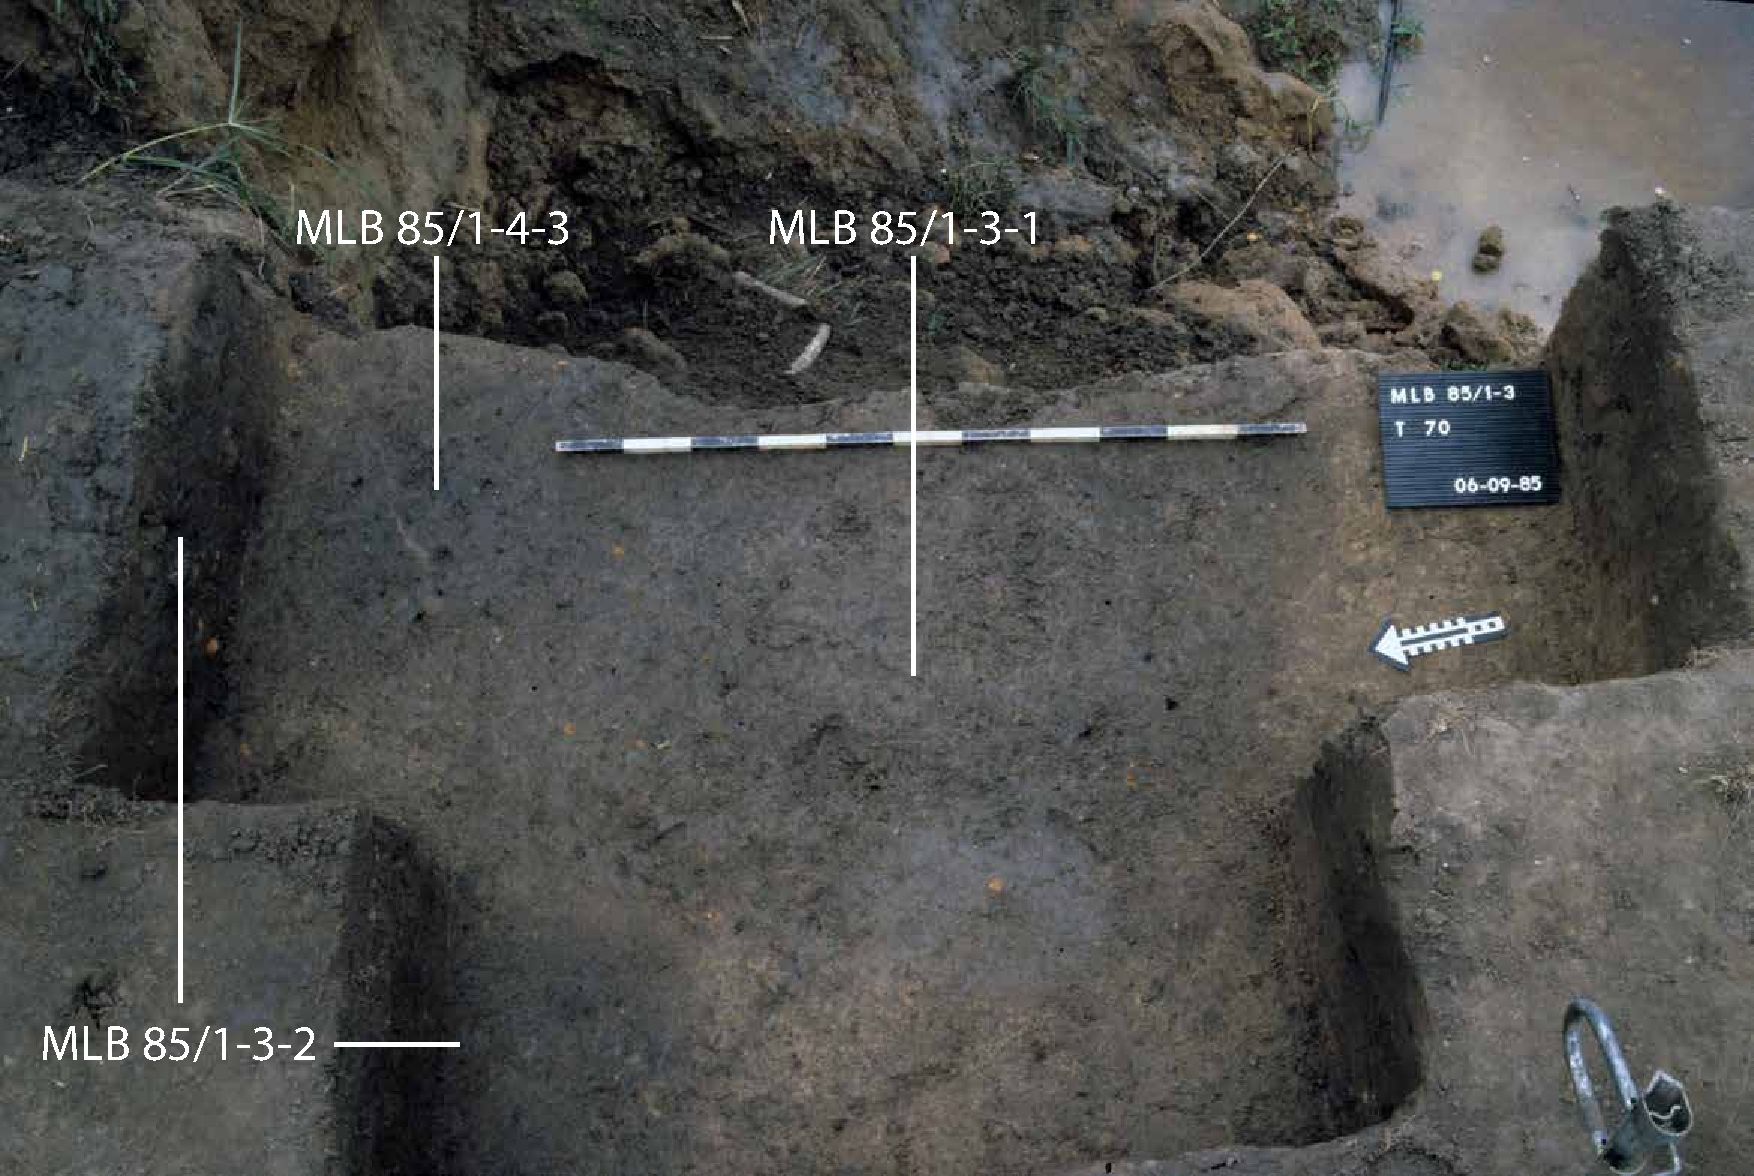
\includegraphics[width=\columnwidth]{fig/MLB85-1-3_T70_E85-031-1_kompr.pdf}
 \caption{Planum 3 (0,45\,m u.~Obfl.)}
 \label{fig:MLB85_1_PlanaT70}
 \end{subfigure}\hfill
 \begin{subfigure}{\columnwidth}
 \centering
 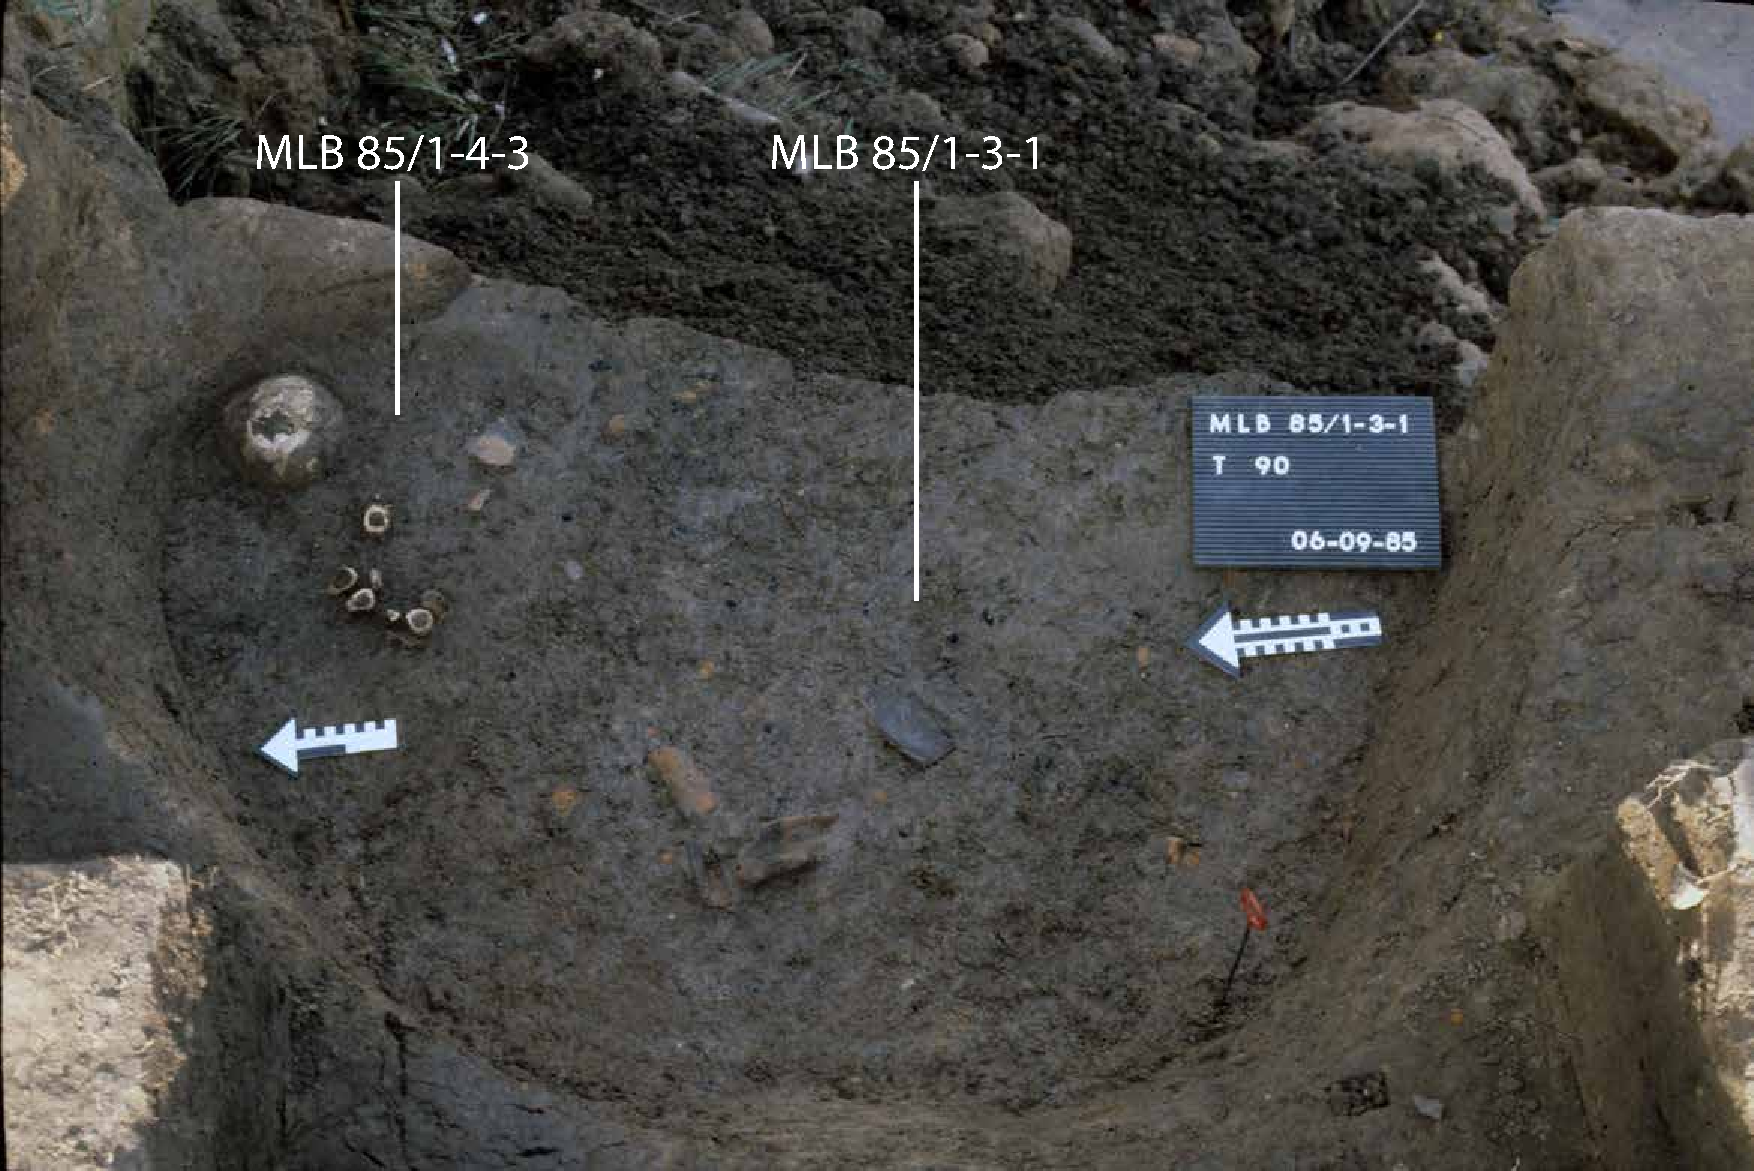
\includegraphics[width=\columnwidth]{fig/MLB85-1-3-1_T90_E85-031-15_kompr.pdf}
 \caption{Planum 4 (0,60\,m u.~Obfl.)}
 \label{fig:MLB85_1_PlanaT90}
\end{subfigure}
 \caption{MLB 85/1: Planum 3 und 4 (Fotos: M. K. H. Eggert, 1985).}
 \label{fig:MLB85_1_PlanaT70+90_Foto}
\end{figure*}

\begin{table*}[p]
	\centering
	%	%\begin{minipage}{.66\textwidth}
	{\footnotesize \begin{sftabular}{@{}lrrrr@{}}
\toprule
   \textbf{Fundkategorie} &  \textbf{Anzahl} &    \textbf{\%} &  \textbf{Gewicht (kg)} &    \textbf{\%} \\
\midrule
 gebrannter Lehm &       1 &   0,3 &          0,10 &   2,0 \\
         Keramik &     305 &  99,0 &          4,49 &  95,7 \\
           Stein &       2 &   0,6 &          0,11 &   2,3 \\
\bottomrule
\end{sftabular}}
	\caption{MLB~85/1-3-1: Anteil verschiedener Fundmaterialien.}
	\label{tab:MLB85-1-3-1_Funde}
	%	%\end{minipage}
\end{table*}

% MLB 85/102 == MLB 85/1-3-1
\paragraph{Grabung und Befunde}\hspace{-.5em}|\hspace{.5em}%
Die Prospektionen in Maluba erbrachten eine Reihe von Gruben. Ausgrabungen an zwei getrennten Stellen innerhalb des Dorfes fanden im Anschluss an die Prospektion des Lua statt. Im etwa 3--4\,m hohen, tonigen Uferprofil des Lua wurden die Reste von vier teilweise freierodierten, tiefen Gruben untersucht: zwei Gruben mit Keramik der Batalimo-Maluba-Gruppe (Kat.-Nr.~1--2) sowie zwei weitere mit (sub)rezentem Fundmaterial (Kat.-Nr.~4--5).\footnote{Nach schweren Regenfällen stürzte die Grabung MLB~85/2 (Kat.-Nr.~4) teilweise ein. Im Anschluss wurde ausschließlich die Grabung MLB~85/1, in welcher die beiden Gruben MLB~85/1-3-1 (Kat.-Nr.~1) und MLB~85/1-3-2 (Kat.-Nr.~2) erfasst wurden, fortgeführt. Die Grabung MLB~85/1 erfasste auch die jüngere Sekundärbestattung MLB~85/1-4-3 (Kat.-Nr.~3). An mehreren Stellen im Dorf wurden an der Oberfläche sichtbare Skelettreste beobachtet. Diese waren den Einwohnern auf Nachfrage hin bekannt.} Im Zuge der ursprünglichen Prospektion in Maluba wurde die spätere Grabungsstelle MLB~85/1 als Survey-Komplex MLB~85/102 aufgenommen.\footnote{Im Verlauf der Bearbeitung zeigte sich, dass die Funde aus dem Survey-Komplex MLB~85/102 Teil der Grube MLB~85/1-3-1 sind. Während der Grabung in Schnitt MLB~85/1 wurde eine weitere Grube zuerst angeschnitten und später unter der Bezeichnung MLB~85/1-3-2 (Kat.-Nr.~2) ebenfalls ausgegraben.} Der Befund war durch einen Erdrutsch freigelegt worden und die Abbruchkante des Uferprofils war zum Zeitpunkt der Grabung etwa 3\,m vom eigentlichen Ufer entfernt und lag mehr als 4,5\,m über dem Wasserspiegel.

Die unter der Kennung MLB~85/1-3-1 ausgegrabene Grube ist kesselförmig und war bis etwa 1,1\,m unter die rezente Oberfläche erhalten (Abb.~\ref{fig:MLB85_1_Zeichnung}). Sie hat einen Durchmesser von zirka 1,5\,m, die Wandungen sind vertikal bis steilschräg überkippt und die Sohle konvex bis wellig mit fließenden Ecken. Die Befundgrenzen sind verwaschen bis fließend und waren aufgrund von Bioturbation schwer zu erfassen. Die ursprüngliche Oberfläche lässt sich nicht mehr rekonstruieren. Im oberen Bereich des erhaltenen Profils ist eine zirka 0,3\,m mächtige dunkle Lage erkennbar (Abb.~\ref{fig:MLB85_1_Zeichnung}: Schicht~1), deren Farbe sich nicht von jener der Grubenfüllung unterscheidet. In dieser Schicht fand sich fast 1/3 der insgesamt aus dem Befund vorliegenden Batalimo-Maluba-Keramik sowie Vertreter anderer Stilgruppen (Abb.~\ref{fig:MLB85-1_KeramikStilgruppen}). Dies legt den Schluss nahe, dass es sich um einen in späterer Zeit aufgearbeiteten Teil der Grube handelt.

An der Unterkante des zweiten Abtrages, bei etwa 0,35\,m unter der rezenten Oberfläche, wurde eine Lage hellen, lehmigen Sediments erfasst. Die eigentlichen Konturen der Grube zeichneten sich erst im dritten Abtrag deutlich ab (Abb.~\ref{fig:MLB85_1_Zeichnung}).\footnote{Ab dieser Tiefe wurden die Abträge nicht mehr bis zu den Grenzen des Grabungsschnittes abgetieft. Nur die eigentliche Verfüllung der Grube in vier weiteren, künstlichen Abträgen ausgegraben.} Im nördlichen Profil des Grabungsschnitts und im westlichen Teil des dritten Planums wurde eine weitere Grube erfasst, die ebenfalls Keramik der Batalimo-Maluba-Gruppe enthielt (MLB~85/1-3-2; Kat.-Nr.~2). Nahe der nordwestlichen Ecke des Schnittes, kurz vor dem Profil, wurden im vierten Abtrag (0,45--0,60\,m u.~Obfl.) ein Schädel und mehrere Langknochen gefunden (Abb.~\ref{fig:MLB85_1_PlanaT70+90_Foto}).\footnote{Der entsprechende Befund wurde unter der Kennung MLB~85/1-4-3 ausgegraben (Kat.-Nr.~3).} Ab dem fünften Abtrag zeichnete sich um die Knochen herum eine deutliche runde Verfärbung ab. Die angelegten Profile ergaben weder eine stratigraphische Relation zwischen den beiden Gruben MLB~85/1-3-1 und MLB~85/1-3-2, noch zwischen der Grube MLB~85/1-3-1 und der Sekundärbestattung MLB~85/1-4-3.\footnote{Es konnte aber festgestellt werden, dass die Sekundärbestattung MLB~85/1-4-3 (Kat.-Nr.~3) in die Verfüllung der Grube MLB~85/1-3-2 (Kat.-Nr.~2) eingreift. Siehe Abb.~\ref{fig:MLB85_1_Zeichnung}: oben, A--B und E--F; \ref{fig:MLB85-143}).}

\vspace{.5em}\noindent Die Grabung erbrachte den folgenden stratigrafischen Befund (Abb.~\ref{fig:MLB85_1_Zeichnung}):
\begin{itemize}[leftmargin=*, labelindent=1.5em, noitemsep, topsep=0pt]
\item [(1)] Deckschicht, 10YR 3/2 bis 3/3, stark humoser, lehmiger Sand
\item [(2)] Grubenverfüllung, 10YR 3/2, stark holzkohlehaltig, humos, lehmiger Sand
\item [(2a)] Angeschnittene Grube MLB~85/1-3-2 (Kat.-Nr.~2), wie (2), 10YR 3/2, lehmiger Sand
\item [(3)] Grubensohle, 10YR 4/3 bis 3/3, fundarm, sandiger Lehm
\item [(4)] Anstehendes, 10YR 5/6, sandiger Lehm
\item [(4a)] Wie (4), 10 YR 5/6 bis 4/3, sandiger Lehm
\item [(5)] Dunkle Linsen aus sandigem Lehm, 10YR 4/3 bis 3/3
\end{itemize}

\begin{figure*}[tb]
	\centering
	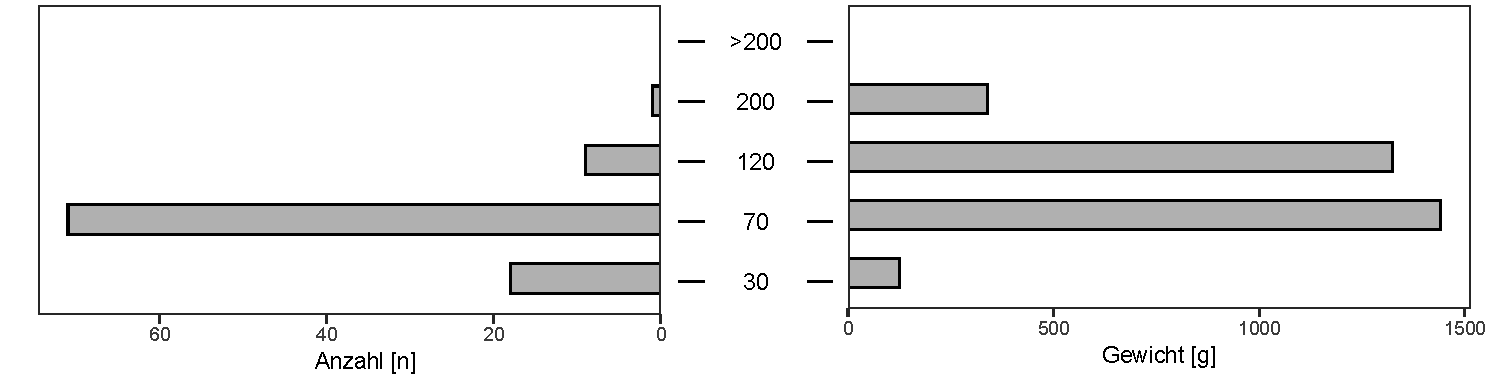
\includegraphics[width=\textwidth]{fig/9-1_MLB85-131_Fragmentierung_2.pdf}
	\caption{MLB~85/1-3-1: Fragmentierungsgrad der Scherben (n~=~99; Größenklassen siehe Anm.~\ref{ftn:Keramik_Fragmentierung}).}
	\label{fig:Fragmenierung_MLB85-131}
\end{figure*}

\columnbreak\paragraph{Keramik\vspace{.5em}}\mbox{}\\
\begin{tabular}{@{}lrl@{}}
Ausgesondert: & 1234\,g & \\
Bearbeitet: & 3228\,g & (72\,\%) \\
Insgesamt: & 4462\,g & \\
\end{tabular} 

\begin{figure*}[p]
	\centering
	\begin{subfigure}[t]{\textwidth}
		\centering
		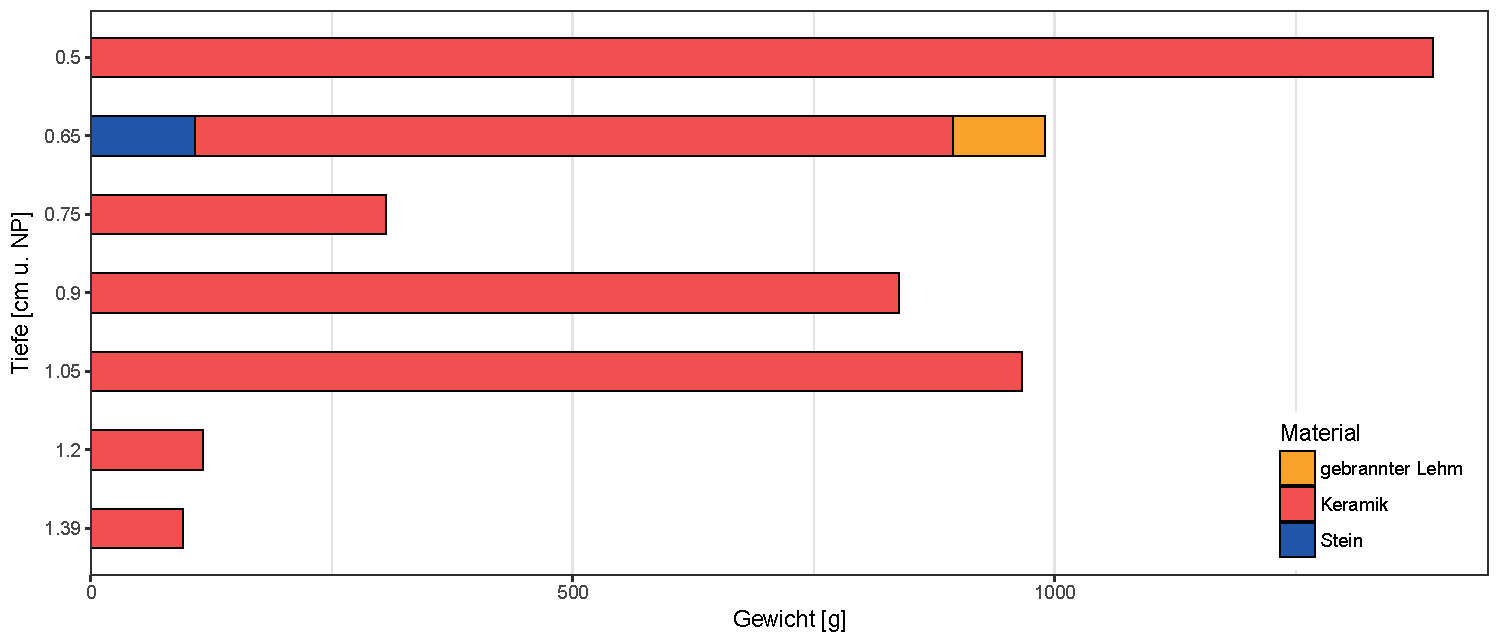
\includegraphics[width=\textwidth]{fig/9-1_MLB85-131_VerteilungFunde_R.pdf}
		\caption{Fundmaterial.\vspace{1em}}
		\label{fig:MLB85-1_VerteilungFunde}
	\end{subfigure}
	\begin{subfigure}[t]{\textwidth}
		\centering
		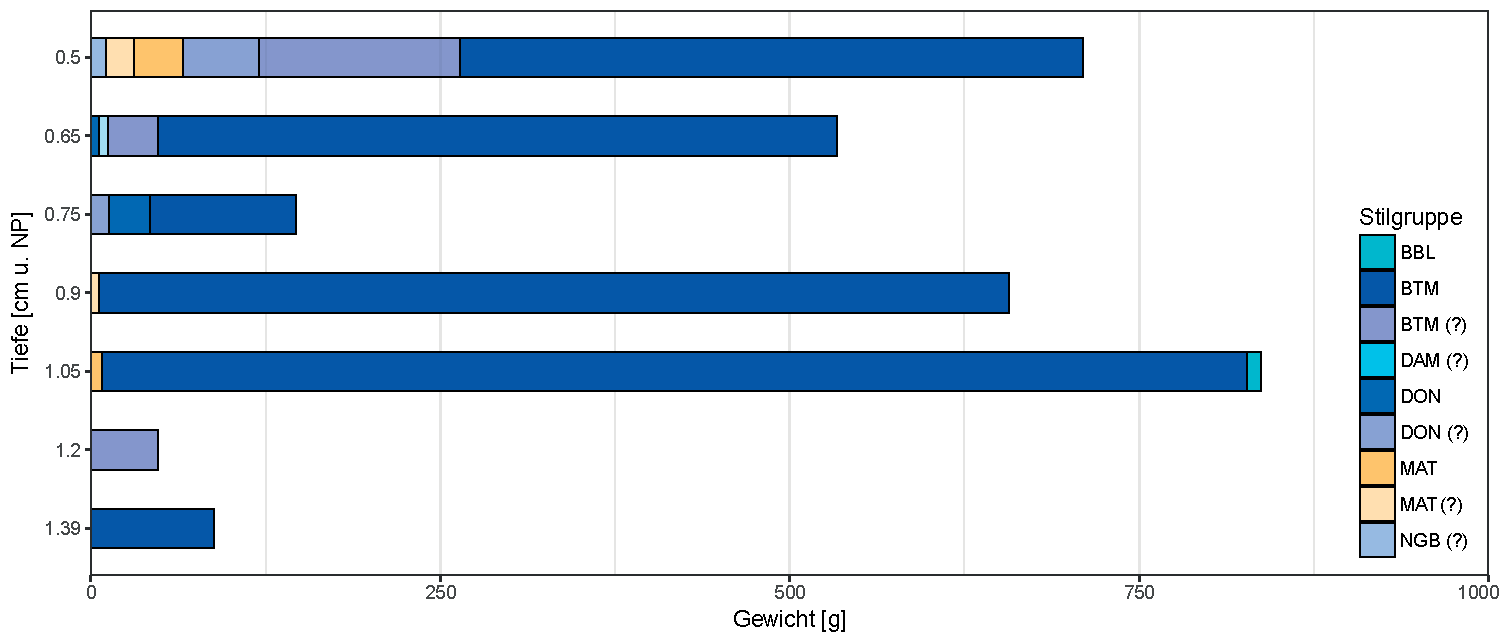
\includegraphics[width=\textwidth]{fig/9-1_MLB85-131_KeramikStilgruppen_R.pdf}
		\caption{Keramische Stilgruppen.\vspace{1em}}
		\label{fig:MLB85-1_KeramikStilgruppen}
	\end{subfigure}
	\begin{subfigure}[t]{\textwidth}
		\centering
		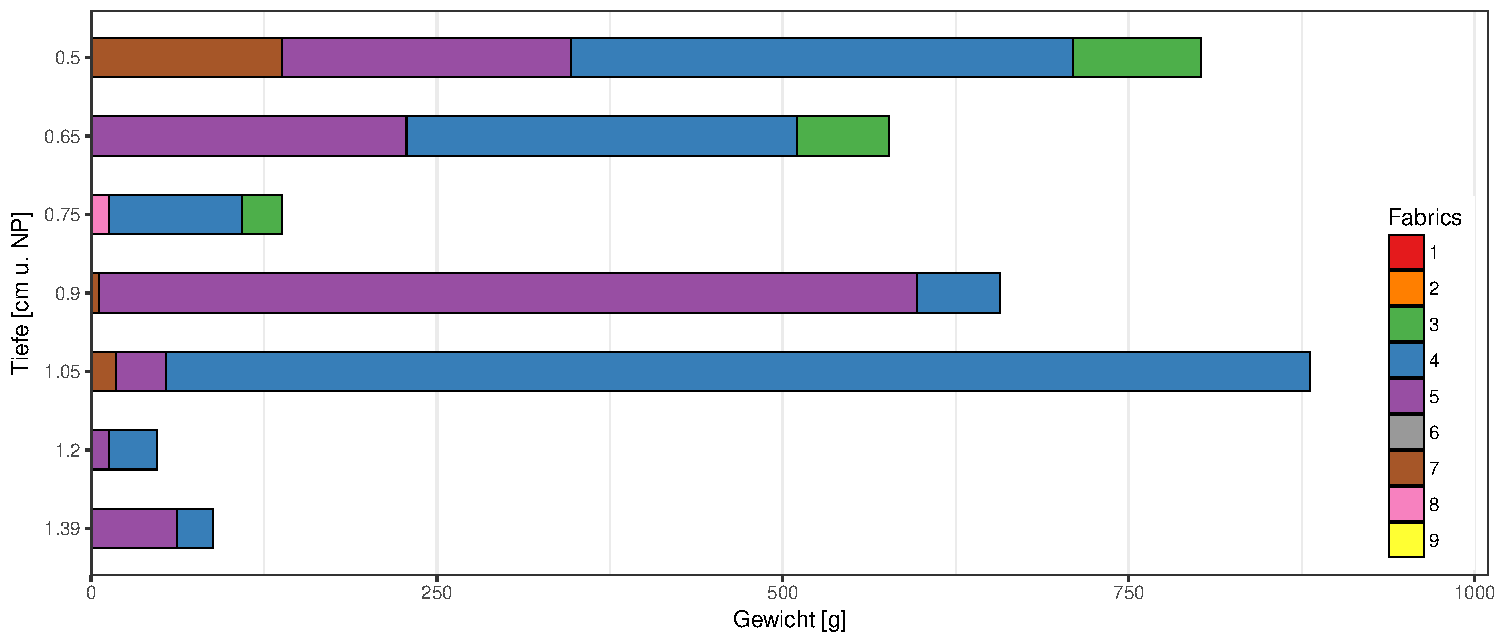
\includegraphics[width=\textwidth]{fig/9-1_MLB85-131_Fabrics_R.pdf}
		\caption{\textit{Fabrics}.}
		\label{fig:MLB85-1_VerteilungFabrics}
	\end{subfigure}
	\caption{MLB 85/1-3-1: Verteilung der Fundmaterialien (A), keramischen Stilgruppen (B) und \textit{Fabrics} (C) in den entsprechenden Tiefen der Grabung.}
	\label{fig:MLB85-1_Verteilung}
\end{figure*}

\vspace{.5em}
\noindent Das Fundmaterial aus der Grube MLB~85/1-3-1 bildet -- zusammen mit jenem aus der benachbarten Grube MLB~85/1-3-2 (Kat.-Nr.~2) -- den Grundstock für den Formenkatalog des Batalimo-Maluba-Stils (Kap.~\ref{sec:BTM-Gr}). Neben der Keramik fand sich ein Stück gebrannten Lehms sowie zwei Steine (Tab.~\ref{tab:MLB85-1-3-1_Funde}). Während der obersten drei Abträge konnten die einzelnen Befunde -- MLB~85/1-3-1, MLB~85/1-3-2 (Kat.-Nr.~2) und MLB~85/1-4-3 (Kat.-Nr.~3) -- nicht unterschieden werden. Die Funde aus diesem Bereich müssen daher als vermischt gelten. Eine Trennung der Funde nach den entsprechenden Komplexen war auch im Rahmen der Auswertung nicht möglich. Das keramische Fundgut ist stark zerscherbt (Abb.~\ref{fig:Fragmenierung_MLB85-131}) und direkte Anpassungen zwischen Scherben ergaben sich äußerst selten (Abb.~\ref{fig:Fragmenierung_MLB85-131}). Dies deutet an, dass es sich bei dem Befund nicht um eine Deponierung von ursprünglich ganzen Gefäßen handelt, sondern dass die Keramik bereits zerscherbt war, als sie in die Grube gelangte. Komplette Gefäße ließen sich kaum rekonstruieren. Die vollständigste Gefäßeinheit (Taf.~25.8) besteht aus 27 Scherben, welche über vier Abträge verteilt sind.\footnote{GE~4 setzt sich aus je zwei Scherben der Abträge 2 und 3 sowie 18 Scherben des 4. und vier weiteren Scherben des 5. Abtrages zusammen.\label{ftn:MLB85-131Refit}}

\begin{table*}[!tb]
	{\footnotesize
		\begin{sftabular}{@{}p{.125\textwidth}p{.125\textwidth}p{.25\textwidth}p{.2\textwidth}p{.15\textwidth}@{}}
			\toprule 
			\textbf{Lab-Nr} & \textbf{Datum (bp)} & \textbf{Datum (2-Sigma)} & \textbf{Abtrag} & \textbf{Tiefe (unter NP)} \\ 
			\midrule 
			GrN-13584 & 1670\( \pm \)110 & 125--605 n.~Chr. & 5 (MLB 85/1-3-1-2; HK 18) & 0,9--1,05\,m \\ 
			KI-2444 & 1930\( \pm \)120 & 342--327 v.~Chr. (0,6\,\%) 204 v.~Chr.--383 n.~Chr. (94,8\,\%) & 7 (MLB 85/1-3-1-4; HK 26) & 1,2--1,39\,m \\ 
			\bottomrule 
	\end{sftabular}}
	\caption{MLB 85/1-3-1: \textsuperscript{14}C-Datierungen.}
	\label{tab:MLB85_1-3-1_14C-Daten}
\end{table*}

\begin{figure*}[!tb]
	\centering
	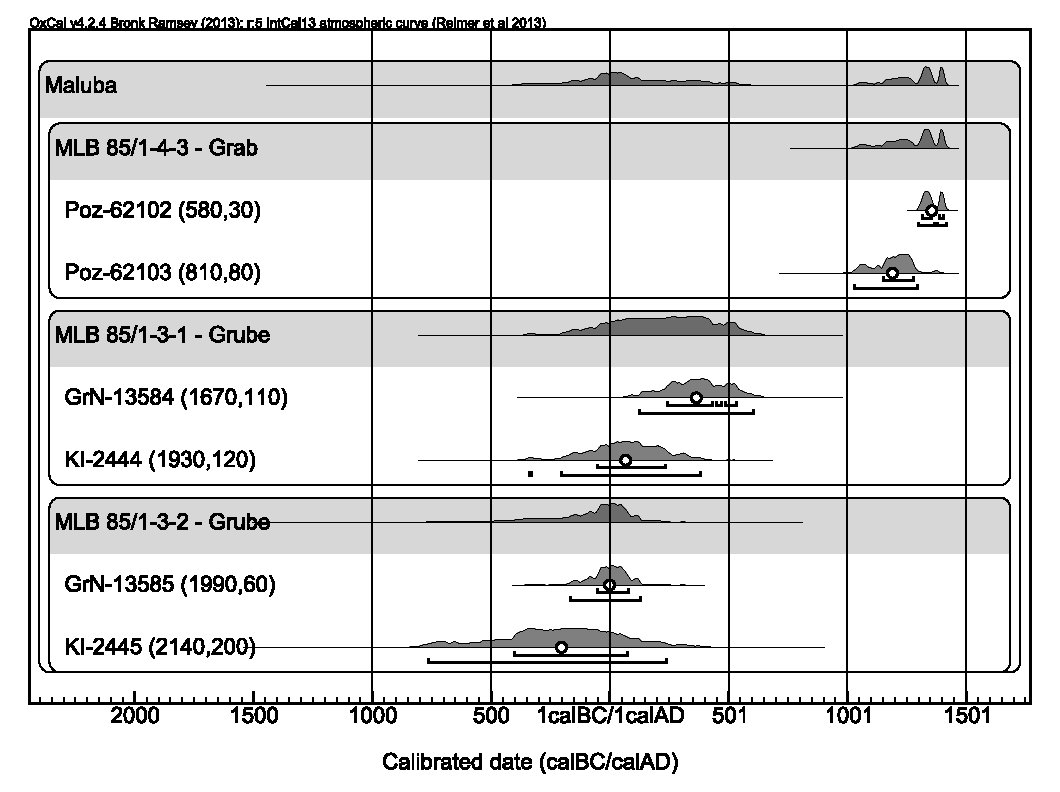
\includegraphics[width = .75\textwidth]{fig/MLB85_14C.pdf}
	\caption{Maluba: Kalibrierung der \textsuperscript{14}C-Datierungen aus den beiden Gruben MLB~85/1-3-1 und MLB~85/1-3-2 sowie der Sekundärbestattung MLB~85/1-4-3 in Maluba am Lua in stratigrafischer Sortierung.}
	\label{fig:MLB85_1_14C-Kalibration}
\end{figure*}

Keramik, insbesondere Vertreter des Batalimo-Maluba-Stils, wurde vor allem in den Abträgen 1--2 und 4--5 gefunden (Abb.~\ref{fig:MLB85-1_Verteilung}). Nach dem fünften Abtrag reduziert sich das Fundaufkommen merklich. Bis in diese Tiefe ist das Inventar mit Scherben durchsetzt, die nicht Teil des Batalimo-Maluba-Stils sind.\footnote{Es handelt sich hierbei um eine GE aus rotbrennenden Tonen mit feiner Matrix (\textit{Fabric} 7) mit sehr kurzen, umgelegten Rändern des Matoto-Stils (Abb.~\ref{fig:MLB85-1_VerteilungFabrics}, Kap.~\ref{sec:MAT-Gr}). In den oberen drei Abträgen fanden sich zudem rouletteverzierte Scherben, von denen eine der Dama-Gruppe zugewiesen werden konnte (Abb.~\ref{fig:MLB85-1_KeramikStilgruppen}; Kap.~\ref{sec:DAM-Gr}).} Diese Verteilung beziehungsweise das auffällig geringe Fundaufkommen im dritten Abtrag kann damit erklärt werden, dass der Abtrag etwas flacher als die anderen war und genau die Grenze zwischen der \textit{Deckschicht} (Abb.~\ref{fig:MLB85_1_Zeichnung}:1) und dem noch erhalten Abschnitt der Grubenverfüllung (2--3) abdeckt. Mit dem vierten Abtrag wurde die Grubenverfüllung ausgegraben, die nunmehr lediglich durch die Sekundärbestattung MLB~85/1-4-3 (Kat.-Nr.~3) gestört war. Der Umstand, dass Anpassungen zwischen Scherben aus dem zweiten bis fünften Abtrag beobachtet wurden\footnote{Siehe Anm.~\ref{ftn:MLB85-131Refit}.}, zeigt an, dass die Abträge 1--3 umgelagertes Grubensediment widerspiegeln. Diese Bereiche sind auch regelhaft mit jüngeren Scherben der Stile Dongo (Kap.~\ref{sec:DON-Gr}), Bobulu (Kap.~\ref{sec:BBL-Gr}), Dama (Kap.~\ref{sec:DAM-Gr}) und Matoto (Kap.~\ref{sec:MAT-Gr}) durchsetzt. Der dritte Abtrag kann als \textit{Störungszone} interpretiert werden. In dieser Tiefe wurde die ursprüngliche Grube mutmaßlich gekappt. Im Profil ist eine deutliche Grenze zwischen den Schichten 1 und 2 (Abb.~\ref{fig:MLB85_1_Zeichnung}) sichtbar. Unterhalb dieser findet sich auffällig viel Holzkohle. 

Das keramische Inventar des Befunds MLB~85/1-3-1 umfasst 99~GE. Aufgrund der starken Fragmentierung ergaben nur zwei GE hinreichend viel Material, um sie als Gefäße anzusprechen. Das Gros bilden 45 Randscherben und 49 Wandungsscherben. Zudem konnten drei Bodenscherben identifiziert werden. Die individuell aufgenommenen GE repräsentieren etwas über 70\,\% des keramischen Materials aus dem Befund.\footnote{Die restlichen, lediglich ausgezählten Scherben sind nicht signifikant oder zeigen nur schlecht ansprechbare Verzierungselemente; beispielsweise einzelne Rillen.}\columnbreak

Der Großteil der identifizierten Gefäßformen sind geschlossene Gefäße mit Zylinderhals und ausbiegendem Rand des Typs C2, wie sie für die Batalimo-Maluba-Gruppe typisch sind (Kap.~\ref{sec:BTM-Gr}). Daneben finden sich nur wenige offene Formen. Es handelt sich hierbei hauptsächlich um Schalen des Typs E5. Von insgesamt 34 Randstücken, die dem Batalimo-Maluba-Stil zugerechnet werden können, sind 19 ausbiegende kurze Ränder des Typs B1.1. Sie zeichnen sich regelhaft durch gerillte Randabschlüsse und Rillenzier auf der Innenseite aus. Für die Matoto-Gruppe charakteristische, kurz umgelegte Ränder des Typs A2 ließen sich in sechs Fällen beobachten. Die entsprechenden Stücke stammen ausschließlich aus dem vierten und fünften Abtrag.\footnote{Diese Stücke, obschon es während der Grabung nicht entsprechend gekennzeichnet wurde, sind mit starker Sicherheit Teil der Verfüllung der jüngeren Bestattung MLB~85/1-4-3 (Kat.-Nr.~3).} Verzierungen basieren größtenteils auf unterschiedlichen Rillen und Riefen-Mustern. Vor allem an der Innenseite der Ränder findet sich regelhaft Rillenverzierung. Die in Batalimo recht häufigen Karo- beziehungsweise Schachbrettmuster (\textsc{De Bayle des Hermens} 1975: Taf.~34) kommen in MLB~85/1-3-1 ebenfalls vor, während Winkelmuster deutlich seltener beobachtet wurden.

\paragraph{Sonstige Funde}\hspace{-.5em}|\hspace{.5em}%
Im zweiten Abtrag fand sich wenig Holzkohle und etwas verziegelter Lehm (Abb.~\ref{fig:MLB85-1_VerteilungFunde}). Ein Stück gebrannter Hüttenlehm weist deutliche konkave Abdrücke auf und kann als Wandbewurf gedeutet werden.\footnote{Siehe auch Diskussion unten im Zusammenhang mit dem in der Grube MLB~85/1-3-2 (Kat.-Nr.~2) gefundenen Hüttenlehm.} Zudem wurden zwei kleine Sandsteinfragmente ausgegraben, die zusammen nur etwa 100\,g wiegen und keine Bearbeitungsspuren zeigen.

\begin{figure*}[!tb]
	\begin{subfigure}{0.37\textwidth}
		\centering
		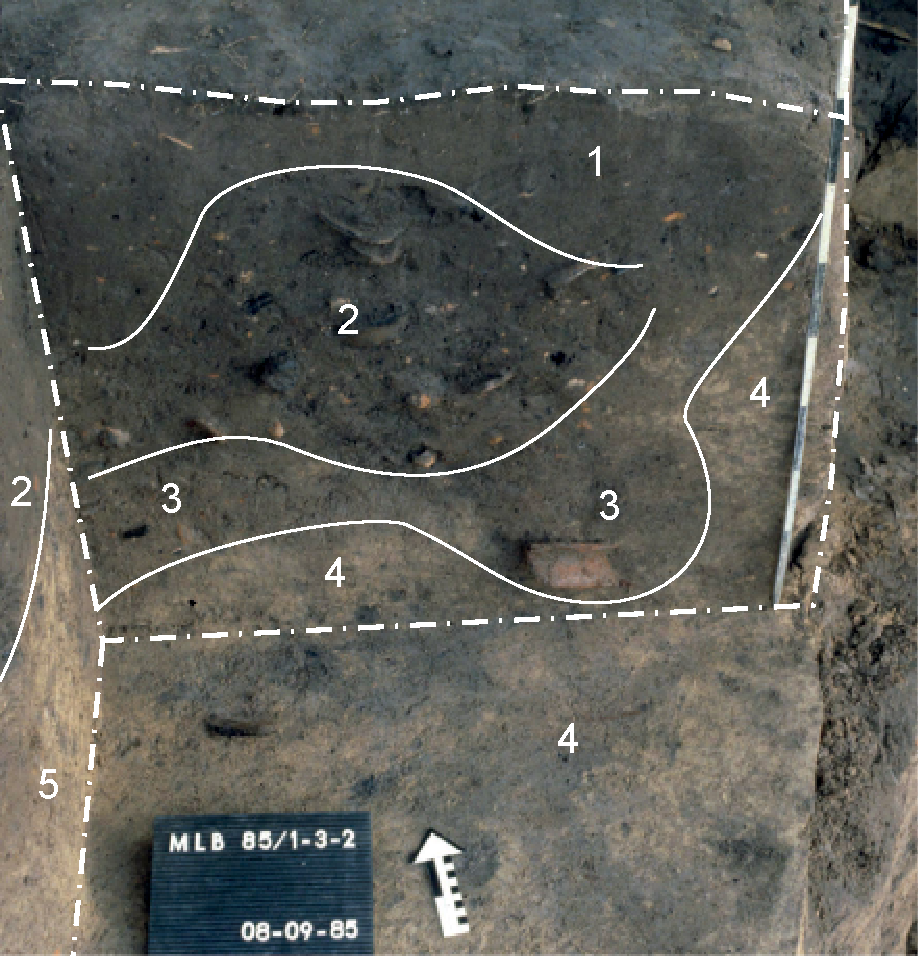
\includegraphics[width=\textwidth]{fig/MLB85-132_E85-032-23.pdf}
		\caption{West--Ost-Profil}
		\label{fig:MLB85-132_W-O-Prof}
	\end{subfigure}\hspace{0.01\textwidth}
	\begin{subfigure}{0.61\textwidth}
		\centering
		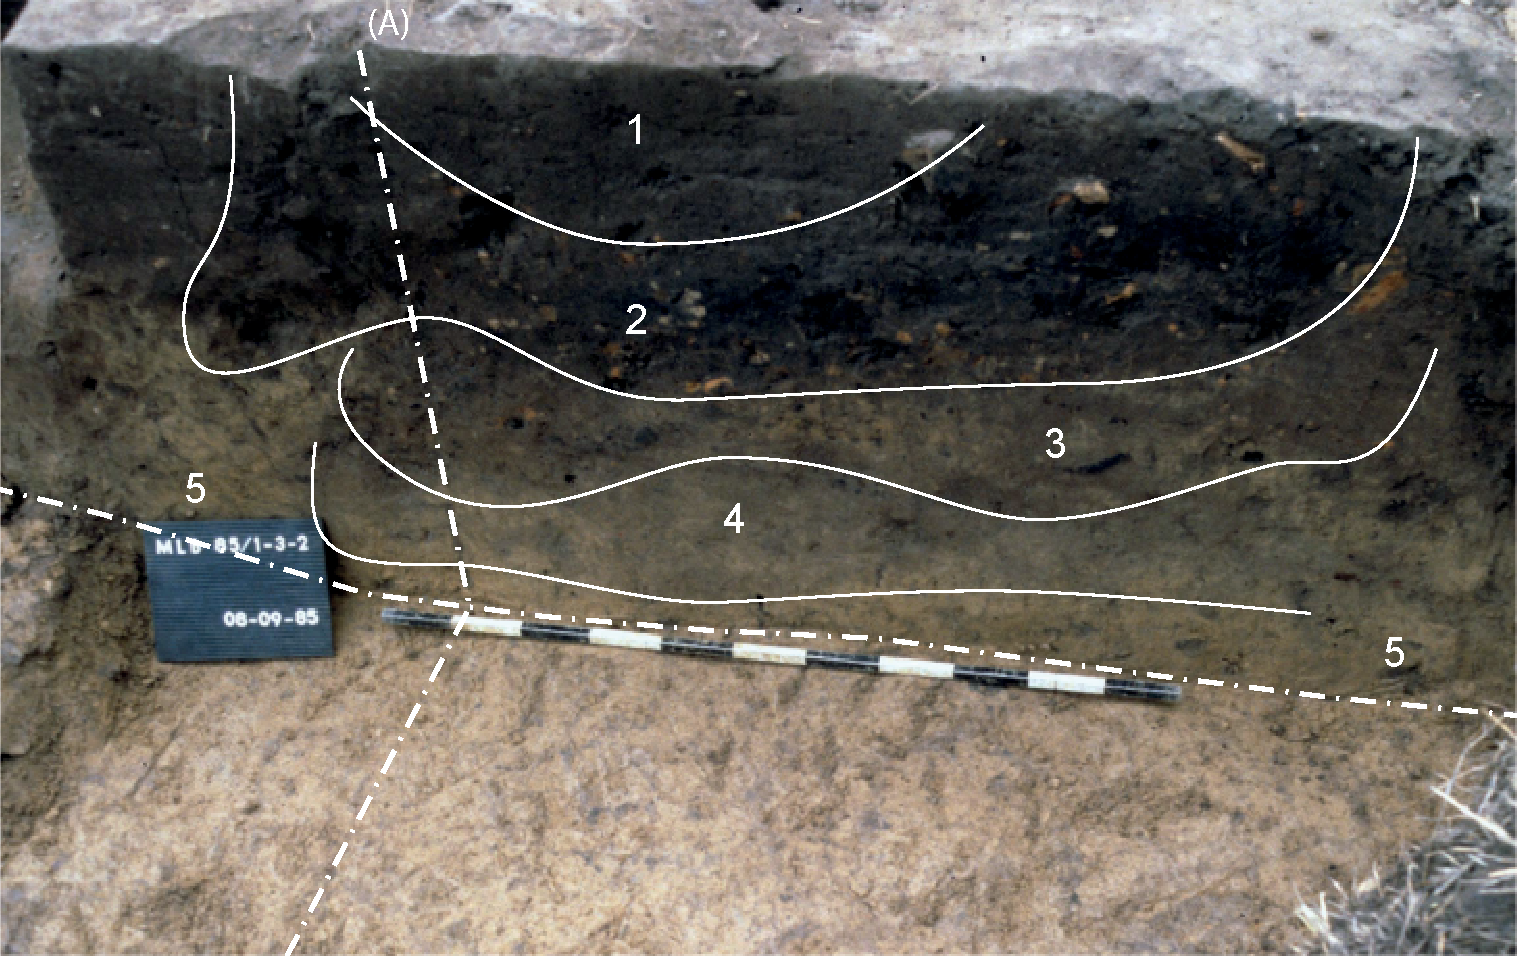
\includegraphics[width=\textwidth]{fig/MLB85-132_E85-032-27.pdf}
		\caption{Nord--Süd-Profil}
		\label{fig:MLB85-132_N-S-Prof}
	\end{subfigure}
	\caption{MLB~85/1-3-2: West--Ost-orientiertes Profil (A) und Süd--Nord-orientiertes Profil durch den Befund bei Grabungsabschluss (B). Zur Lage der Profile siehe auch Abb.~\ref{fig:MLB85_1_Zeichnung} (Fotos: M. K. H. Eggert, 1985).}
	\label{fig:MLB85-1-3-2_NordProfil}
\end{figure*}

\paragraph{Datierung}\hspace{-.5em}|\hspace{.5em}%
Je eine Probe für Radiokohlenstoffdatierungen wurde im fünften wie siebten Abtrag genommen (Tab.~\ref{tab:MLB85_1-3-1_14C-Daten}). Beide absolute Datierungen decken einen Bereich zwischen dem 4.~Jh. v.~Chr. bis 6.~Jh. n.~Chr. ab. Während die Probe aus dem fünften Abtrag (GrN-13584) etwas jünger als die aus dem siebten Abtrag stammende Probe (KI-2444) datiert, überlagern sich beide Proben im kalbierten 2-Sigma-Intervall. Für den Befund MLB~85/1-3-1 lässt sich eine Datierung in die erste Hälfte des 1.~Jt. n.~Chr. als am Wahrscheinlichsten annehmen (Abb.~\ref{fig:MLB85_1_14C-Kalibration}). 

\paragraph{Interpretation}\hspace{-.5em}|\hspace{.5em}%
Die in der Grabung MLB~85/1-3-1 erfasste Grube weist einen Durchmesser von zirka 1,5\,m auf und reicht noch bis zu 1,1\,m unter die rezente Oberfläche. Zum Zeitpunkt der Grabung waren bereits etwa 40\,\% des Befundes erodiert. Die gesamte Grube, vorausgesetzt sie war zylindrisch, müsste in etwa ein Volumen von etwa 1,4\,m\textsuperscript{3} aufgewiesen haben, von denen noch etwa 0,9\,m\textsuperscript{3} erhalten waren. Die Funddichte liegt bei etwa 5\,kg/m\textsuperscript{3} und das Fundaufkommen nimmt zur Sohle hin deutlich ab. Ausreichend gesichert ist die Verfüllung der Grube erst ab einer Tiefe von etwa 0,3\,m unter der rezenten Oberfläche. Ob die Durchmischung im darüber liegenden Bereich das Ergebnis jüngerer Eingrabungen ist, konnte nicht abschließend geklärt werden. Das keramische Fundmaterial aus der Grube ist einer der definierenden Komplexe für die Beschreibung des Batalimo-Maluba-Stils. Die Auswertung ergab keine Hinweise, welche Rückschlüsse auf die Nutzung oder Funktion der Grube zuließen. Charakteristika einer intentionellen Deponierung \parencite[siehe][]{Wotzka.1993} fanden sich nicht.

\section*{\begin{tabular*}{\linewidth}{@{}l @{\extracolsep{\fill}} r@{}}
Nr.~2 & MLB~85/1-3-2\\
\end{tabular*} 
}

\textsf{\textbf{Maluba (Lua; Fpl.~230)}}

\vspace{1em}

\noindent\begin{tabular}{@{}rl@{}}
\textbf{Feldarbeit:} & \textbf{08.09.1985 (F. Nikulka)} \\ 
\textbf{Abb.:} & \textbf{\ref{fig:MLB85-1-3-2_NordProfil}--\ref{fig:Fragmenierung_MLB85-132}} \\
\textbf{Tab.:} & \textbf{\ref{tab:MLB85-1-3-2_Funde}--\ref{tab:MLB85_1-3-3_14C-Daten}}\\
\textbf{Taf.:} & \textbf{26.9--27.8} \\ 
\textbf{Lit.:} & \textbf{\textsc{Eggert}~1987b} \\ 
\end{tabular}

% NOTES: MLB 85/104 == MLB 85/1-3-2

\paragraph{Grabung und Befunde}\hspace{-.5em}|\hspace{.5em}%
Direkt nordwestlich der Grube MLB~85/1-3-1 (Kat.-Nr.~1) wurde eine weitere, teilweise frei erodierte Grube erfasst.\footnote{Die abgesammelten Funde erhielten die Bezeichnung MLB~85/104. Aus dem Survey-Inventar stammt ein fragmentiertes Gefäß der Batalimo-Maluba-Gruppe (Taf.~26.9).} Während der Ausgrabung von MLB~85/1-3-1 wurde der Befund angeschnitten und als Komplex MLB~85/1-3-2 untersucht (Abb.~\ref{fig:MLB85_1_Zeichnung}--\ref{fig:MLB85_1_PlanaT70}). Im Zuge der Ausgrabung konnte die stratigraphische Relation zwischen den beiden Gruben nicht erfasst werden.\footnote{Während der Ausgrabung der Sekundärbestattung MLB~85/1-4-3 (Kat.-Nr.~3) wurde beobachtet, dass diese in die Verfüllung der Grube MLB~85/1-3-2 eingreift, also stratigraphisch jünger ist (Abb.~\ref{fig:MLB85-143}).} Die wannenförmige, bis etwa 0,7\,m unter die heutige Oberfläche reichende Grube MLB~85/1-3-2 hat steilschräge bis schräge Wandungen, die fließend in eine konvexe Sohle übergehen (Abb.~\ref{fig:MLB85-1-3-2_NordProfil}). Die Befundgrenzen sind verwaschen bis fließend.\footnote{Im Vergleich zu den scharfen Befundgrenzen der Gruben MLB~85/2 und MLB~85/103 (Kat.-Nr.~4--5) zeigen die verwaschenen Grenzen das höhere Alter der beiden, Keramik des Batalimo-Maluba-Stils enthaltenen Gruben MLB~85/1-3-1 und MLB~85/1-3-2 (Kat.-Nr.~1--2).} Im Gelände wurden keine \textit{Verfüllschichten} beschrieben, die vorliegenden Fotos legen jedoch mindestens vier unterschiedliche Verfüllpakete mit konvexen bis welligen Schichtgrenzen nahe (Abb.~\ref{fig:MLB85-1-3-2_NordProfil}).\columnbreak

\begin{table*}[tb]
	\centering
	{\footnotesize \begin{sftabular}{@{}lrrrr@{}}
\toprule
   \textbf{Fundkategorie} &  \textbf{Anzahl} &    \textbf{\%} &  \textbf{Gewicht (kg)} &    \textbf{\%} \\
\midrule
 gebrannter Lehm &       2 &   1,8 &          0,40 &  11,9 \\
         Keramik &     108 &  97,3 &          2,72 &  81,0 \\
           Stein &       1 &   0,9 &          0,24 &   7,1 \\
\bottomrule
\end{sftabular}
}
	\caption{MLB~85/1-3-2: Anteil verschiedener Fundmaterialien.}
	\label{tab:MLB85-1-3-2_Funde}
\end{table*}

Im zweiten Abtrag wurde im nördlichen Bereich eine ausgeprägte Holzkohlekonzentration erfasst. Unterhalb des dritten Abtrages, ab einer Tiefe von etwa 0,4--0,5\,m unter der Oberfläche ging die dunkle, schwarze Kernverfüllung (Abb.~\ref{fig:MLB85-1-3-2_NordProfil}: Schicht~2) langsam in einen braun-gelben, inhomogenen Mischbereich aus sandigem Lehm und Sand über (Abb.~\ref{fig:MLB85-1-3-2_NordProfil}: Schicht~3). Bis zu einer Tiefe von etwa 0,6\,m unter der Oberfläche trat in diesem Mischbereich auch noch Keramik auf. Ab etwa 0,77\,m war die Sohle (Abb.~\ref{fig:MLB85-1-3-2_NordProfil}: Schicht~4) erreicht. Im Planum wurde nur noch der anstehende gelbe Lehm beobachtet. Die Schichten~1--4 entsprechen in etwa den Niveaus der künstlichen Abträge.

\vspace{.5em}\noindent Nach der vorliegenden Fotodokumentation lässt sich folgender stratigrafischer Befund ableiten:\footnote{Im Gelände wurden Plana und Profile nicht beschrieben und auch gezeichnet.}
\begin{itemize}[leftmargin=*, labelindent=0.5em, noitemsep, topsep=0pt]
	\item [(1)] Stark dunkelgrauer, homogener Bereich (rezenter Oberboden oder Verfüllungsbereich); wenige Funde.
	\item [(2)] Dunkelgraue bis schwarze, fleckige Schicht mit hohem Fundaufkommen, durchzogen von etwa 0,1--0,2 m dicken, tief dunklen/schwarzen Bändern; enthält viele ziegelrote Brocken.
	\item [(3)] Hellgraue, fleckige Schicht; Mischbereich aus sandigem Lehm und Sand; enthält Hüttenlehm und Holzkohle.
	\item [(4)] Leicht vergraute Grubensohle; im Profil sind keine/kaum Funde sichtbar.
	\item [(5)] Anstehender, gelber Lehm.
\end{itemize}

\paragraph{Keramik\vspace{.5em}}\mbox{}\\
\begin{tabular}{@{}lrl@{}}
Ausgesondert: & 459\,g & \\
Bearbeitet: & 2263\,g & (83\,\%) \\
Insgesamt: & 2722\,g & \\
\end{tabular} 

\begin{figure*}[p]
	\centering
	\begin{subfigure}[t]{\textwidth}
		\centering
		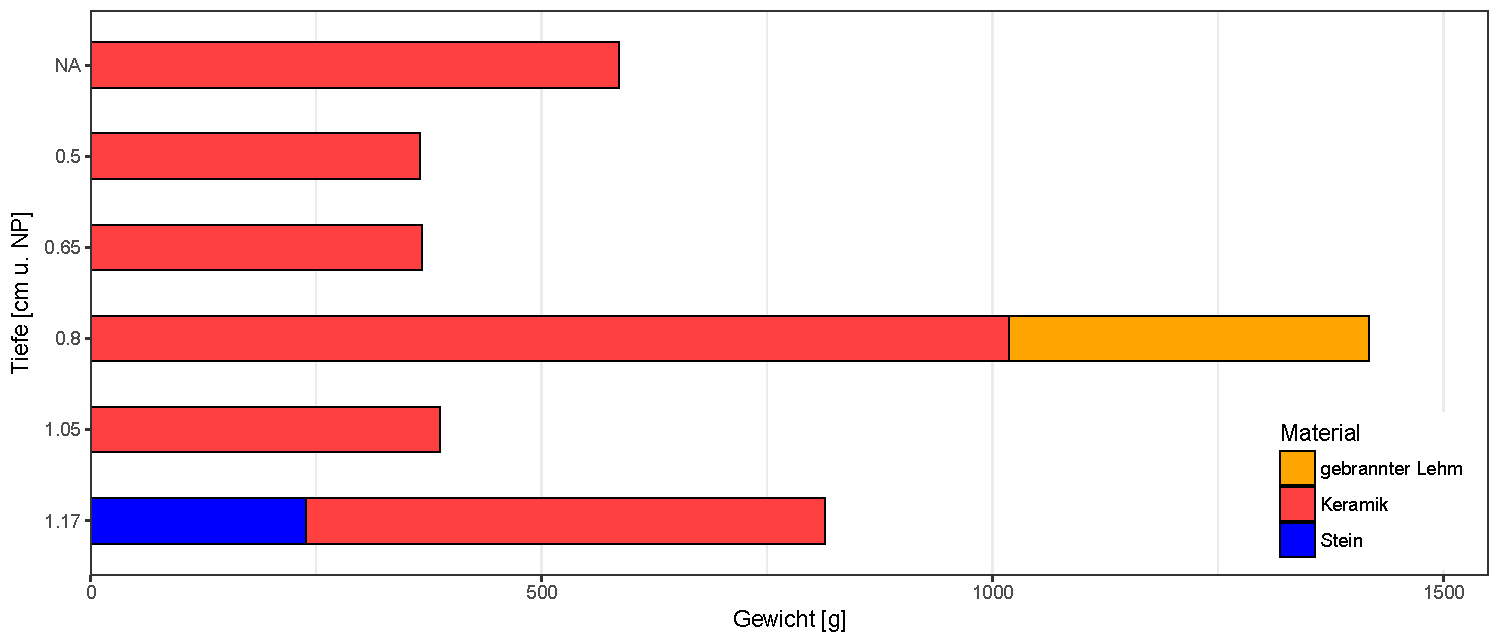
\includegraphics[width=\textwidth]{fig/9-2_MLB85-132_VerteilungFunde_R.pdf}
		\caption{Fundmaterial.\vspace{1em}}
		\label{fig:MLB85-132_VerteilungFunde}
	\end{subfigure}
	\begin{subfigure}[t]{\textwidth}
		\centering
		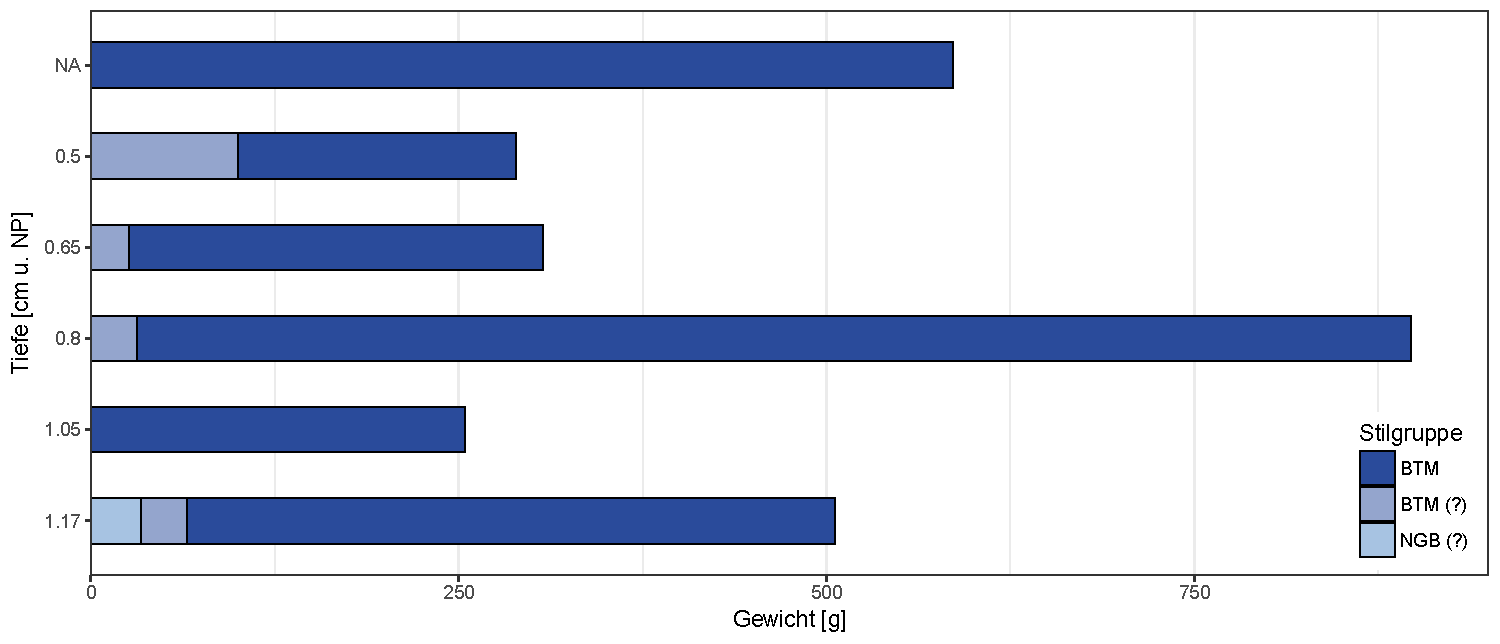
\includegraphics[width=\textwidth]{fig/9-2_MLB85-132_KeramikStilgruppen_R.pdf}
		\caption{Keramische Stilgruppen.\vspace{1em}}
		\label{fig:MLB85-132_KeramikStilgruppen}
	\end{subfigure}
	\begin{subfigure}[t]{\textwidth}
		\centering
		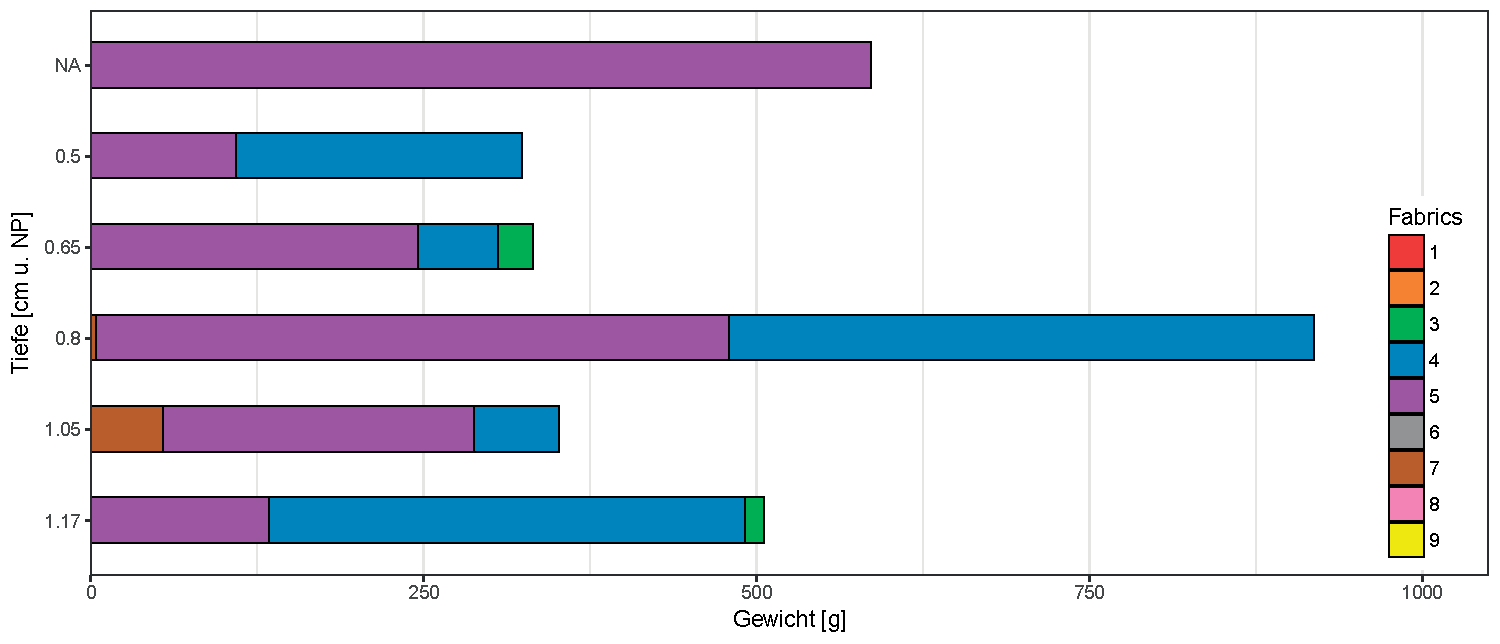
\includegraphics[width=\textwidth]{fig/9-2_MLB85-132_Fabrics_R.pdf}
		\caption{\textit{Fabrics}.}
		\label{fig:MLB85-132_VerteilungFabrics}
	\end{subfigure}
	\caption{MLB 85/1-3-2: Verteilung der Fundmaterialien (A), keramischen Stilgruppen (B) und \textit{Fabrics} (C) in den entsprechenden Tiefen der Grabung.}
	\label{fig:MLB85-132_Verteilung}
\end{figure*}

\vspace{1em}
\noindent Das keramische Inventar aus dem Befund MLB~85/1-3-2 kann bis auf ein Fragment komplett der Batalimo-Maluba-Gruppe (Kap.~\ref{sec:BTM-Gr}) zugerechnet werden. Es gibt nur sehr wenige, nicht näher ansprechbare Scherben, die eventuell jüngeren Gruppen angehören. Die Keramik bildet, zusammen mit jener aus der direkt benachbarten Grube MLB~85/1-3-1 (Kat.-Nr.~1), den Grundstock für den Formenkatalog des Batalimo-Maluba-Stils. Die einzeln aufgenommenen, diagnostischen GE repräsentieren mehr als 80\,\% des Inventars aus der Grube. Das Gros der Funde lag an der Sohle der dunklen, stark heterogenen Schicht~2, die bis etwa 0,44\,m unter die Oberfläche reichte und vor allem im dritten Abtrag erfasst wurde (Abb.~\ref{fig:MLB85-132_VerteilungFunde}). Die darunter liegende, hellere, durchmischte Schicht~3 beziehungsweise der vierte Abtrag erbrachte weniger Fundmaterial. An der Sohle der Grube steigt das Keramikaufkommen wieder leicht an.\footnote{Im West--Ost durch den Befund laufenden Profil (Abb.~\ref{fig:MLB85-132_W-O-Prof}) ist in dieser Schicht der Rand einer Schale des Typs E5 zu erkennen.}

\begin{figure*}[tb!]
	\centering
	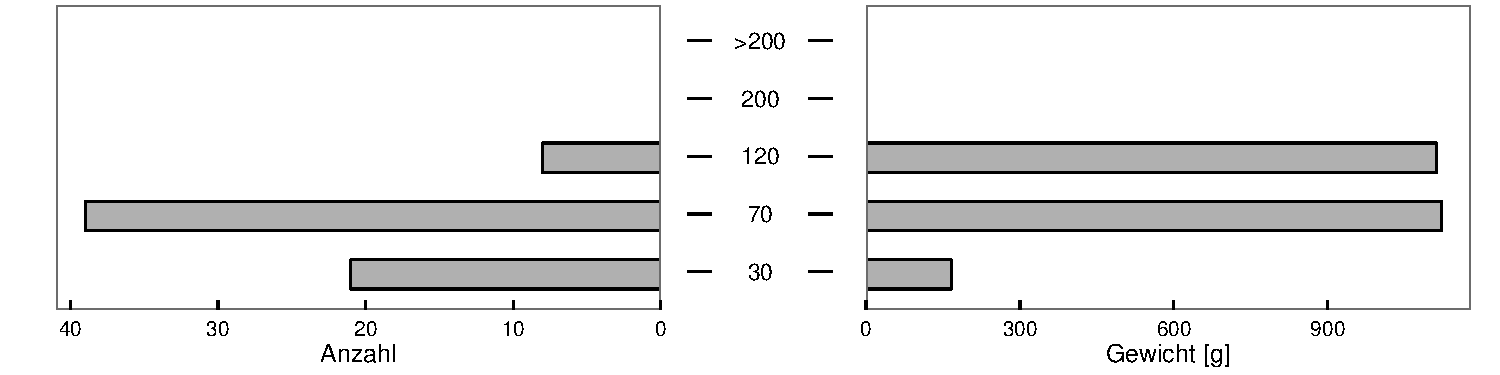
\includegraphics[width=\textwidth]{fig/9-2_MLB85-132_Fragmentierung_2.pdf}
	\caption{MLB~85/1-3-2: Fragmentierungsgrad der Scherben (n~=~68; Größenklassen siehe Anm.~\ref{ftn:Keramik_Fragmentierung}).}
	\label{fig:Fragmenierung_MLB85-132}
\end{figure*}

\begin{table*}[tb!]
	\vspace{1em}
	\centering
	{\footnotesize
		\begin{sftabular}{@{}p{.125\textwidth}p{.125\textwidth}p{.25\textwidth}p{.2\textwidth}p{.15\textwidth}@{}}
			\toprule 
			\textbf{Lab-Nr} & \textbf{Datum (bp)} & \textbf{Datum (2-Sigma)} & \textbf{Abtrag} & \textbf{Tiefe (unter NP)} \\ 
			\midrule 
			KI-2445 & 2140\( \pm \)200 & 764--680 v.~Chr. (3,6\,\%); 674 v.~Chr.--245 n.~Chr. (91,8\,\%) & 3 (MLB~85/1-3-2-3; HK 33) & 0,65--0,8\,m \\ 
			GrN-13585 & 1990\( \pm \)60 & 166 v.~Chr.--129 n.~Chr. & 4 (MLB~85/1-3-2-4; HK 36) & 0,8--1,05\,m \\ 
			\bottomrule 
	\end{sftabular}}
	\caption{MLB 85/1-3-2: \textsuperscript{14}C-Datierungen.}
	\label{tab:MLB85_1-3-3_14C-Daten}
\end{table*}

Wie die Keramik aus dem benachbarten Befund MLB 85/1-3-1 ist auch das Material aus der Grube MLB~85/1-3-2 stark zerscherbt und es ergaben sich nur wenige direkte Anpassungen (Abb.~\ref{fig:Fragmenierung_MLB85-132}). Es fanden sich keine Hinweise, dass einstmals vollständige Gefäße in die Grube gelangt waren. Auch die Rekonstruktion von Gefäßeinheiten auf Basis gemeinsamer formaler und technischer Merkmale war nur in sehr wenigen Fällen sicher möglich. Im fünften Abtrag, unmittelbar an der Sohle der Grube fand sich eine Scherbe, die potenziell der \mbox{Ngbanja}-Gruppe zugerechnet werden kann (Kap.~\ref{sec:NGB-Gr}; Taf.~27.6.).\footnote{Aufgrund der engen formalen Verwandtschaft zwischen \mbox{Ngbanja}- und Batalimo-Maluba-Stil ist die Zuordnung jedoch schwierig.}

Das Inventar aus der Grube besteht aus 68 individuell aufgenommenen GE. Etwa 55\,\% (27~GE) davon sind Randscherben. Zudem umfasst das Inventar noch sieben Bodenscherben und 34 diagnostische Wandungsscherben. Durch die Rekonstruktion von GE konnten elf Gefäße mit geschweifter Wandung, ausgeprägtem Schulter- und Halsbereich des Typs C2 sowie fünf Schalen des Typs E5 identifiziert werden. Die bereits erwähnte, unter Vorbehalt der \mbox{Ngbanja}-Gruppe zugewiesene Schale (Taf.~27.6) kann am ehesten dem Gefäßtyp H2 zugewiesen werden. 13 der insgesamt 27 ansprechbaren Randstücke spiegeln die für die Batalimo-Maluba-Gruppe charakteristischen ausbiegenden, gerillten Ränder des Typs B1.1 wider, die häufig einen leicht konvex ausgearbeiteten Halsbereich abschließen. Ähnlich wie bei der Keramik aus der benachbarten Grube MLB~85/1-3-1 wird das Spektrum der Verzierungen von Rillen- und Riefen bestimmt. Daneben finden sich flächiges Schachbrett sowie Eindruckbänder in fast identischen Anteilen.

\paragraph{Sonstige Funde}\hspace{-.5em}|\hspace{.5em}%
Neben der Keramik fanden sich zwei Stücke gebrannter Lehm, die beide konkave Abdrücke aufweisen. Das größere Fragment weist zwei Abdrücke auf, die durch Stangen mit einem Durchmesser von etwa 15\,cm verursacht wurden. Zwischen diesen Abdrücken liegen auf beiden Seiten weitere, leicht konkave Flächen. Das kleinere Fragment weist zudem einen Abdruck auf, der durch eine Stange mit nur 2,5\,cm Durchmesser erzeugt wurde.

\paragraph{Datierung}\hspace{-.5em}|\hspace{.5em}%
Aus dem Befund MLB~85/1-3-2 liegen zwei \textsuperscript{14}C-Datierungen vor (Tab.~\ref{tab:MLB85_1-3-3_14C-Daten}). Die absolute Datierung des Befundes wird durch die große Standardabweichung einer Probe (KI-2445) erschwert; diese deckt einen Zeitraum vom 8.~Jh. v.~Chr. bis ins 3.~Jh. n.~Chr. ab. Die zweite Probe (GrN-13585) datiert hingegen zuverlässig um die Zeitenwende (Abb.~\ref{fig:MLB85_1_14C-Kalibration}). Als hinreichend sicherer Datierungsansatz ergibt sich ein Zeitraum vom 2.~Jh. v.~Chr. bis in das 2.~Jh. n.~Chr.\footnote{Die kalibrierten Radiokohlenstoffdatierungen aus dem Befund MLB~85/1-3-2 sind etwas älter als die aus der benachbarten Grube MLB~85/1-3-1 (Kat.-Nr.~1; Abb.~\ref{fig:MLB85_1_14C-Kalibration}). Jedoch überschneiden sich die Datierungsansätze beider Gruben nach der Kalibration im 2-Sigma-Bereich. Auch wurde keine stratigrafische Relation zwischen den beiden Gruben beobachtet und das keramische Fundinventar lässt keine Unterschiede erkennen.}

\paragraph{Interpretation}\hspace{-.5em}|\hspace{.5em}%
Die Grube MLB~85/1-3-2 ist der direkt südlich liegenden Grube MLB~85/1-3-1 (Kat.-Nr.~1) sehr ähnlich. Aufgrund des geringen Dokumentationsgrades ist der Befund jedoch nicht detaillierter ansprechbar. Die Grube dürfte bis zirka 0,7\,m unter die heutige Oberfläche gereicht haben, bei einem Durchmesser von fast 2\,m.\footnote{Die Dimensionen des Befundes -- mit Ausnahme der Tiefe -- können nur auf Basis der Fotos abgeschätzt werden, da diese Informationen im Gelände nicht dokumentiert wurden. Durch die Grabung wurde ein etwa 1\,$\times$\,1\,$\times$\,1,4\,m großer Teil der Grube erfasst (siehe Abb.~\ref{fig:MLB85-1-3-2_NordProfil}).} Sie dürfte damit etwa ebenso so groß oder sogar etwas größer als die benachbarte Grube MLB~85/1-3-1 gewesen sein.

\begin{figure*}[tb]
 \begin{subfigure}{\columnwidth}
 \centering
 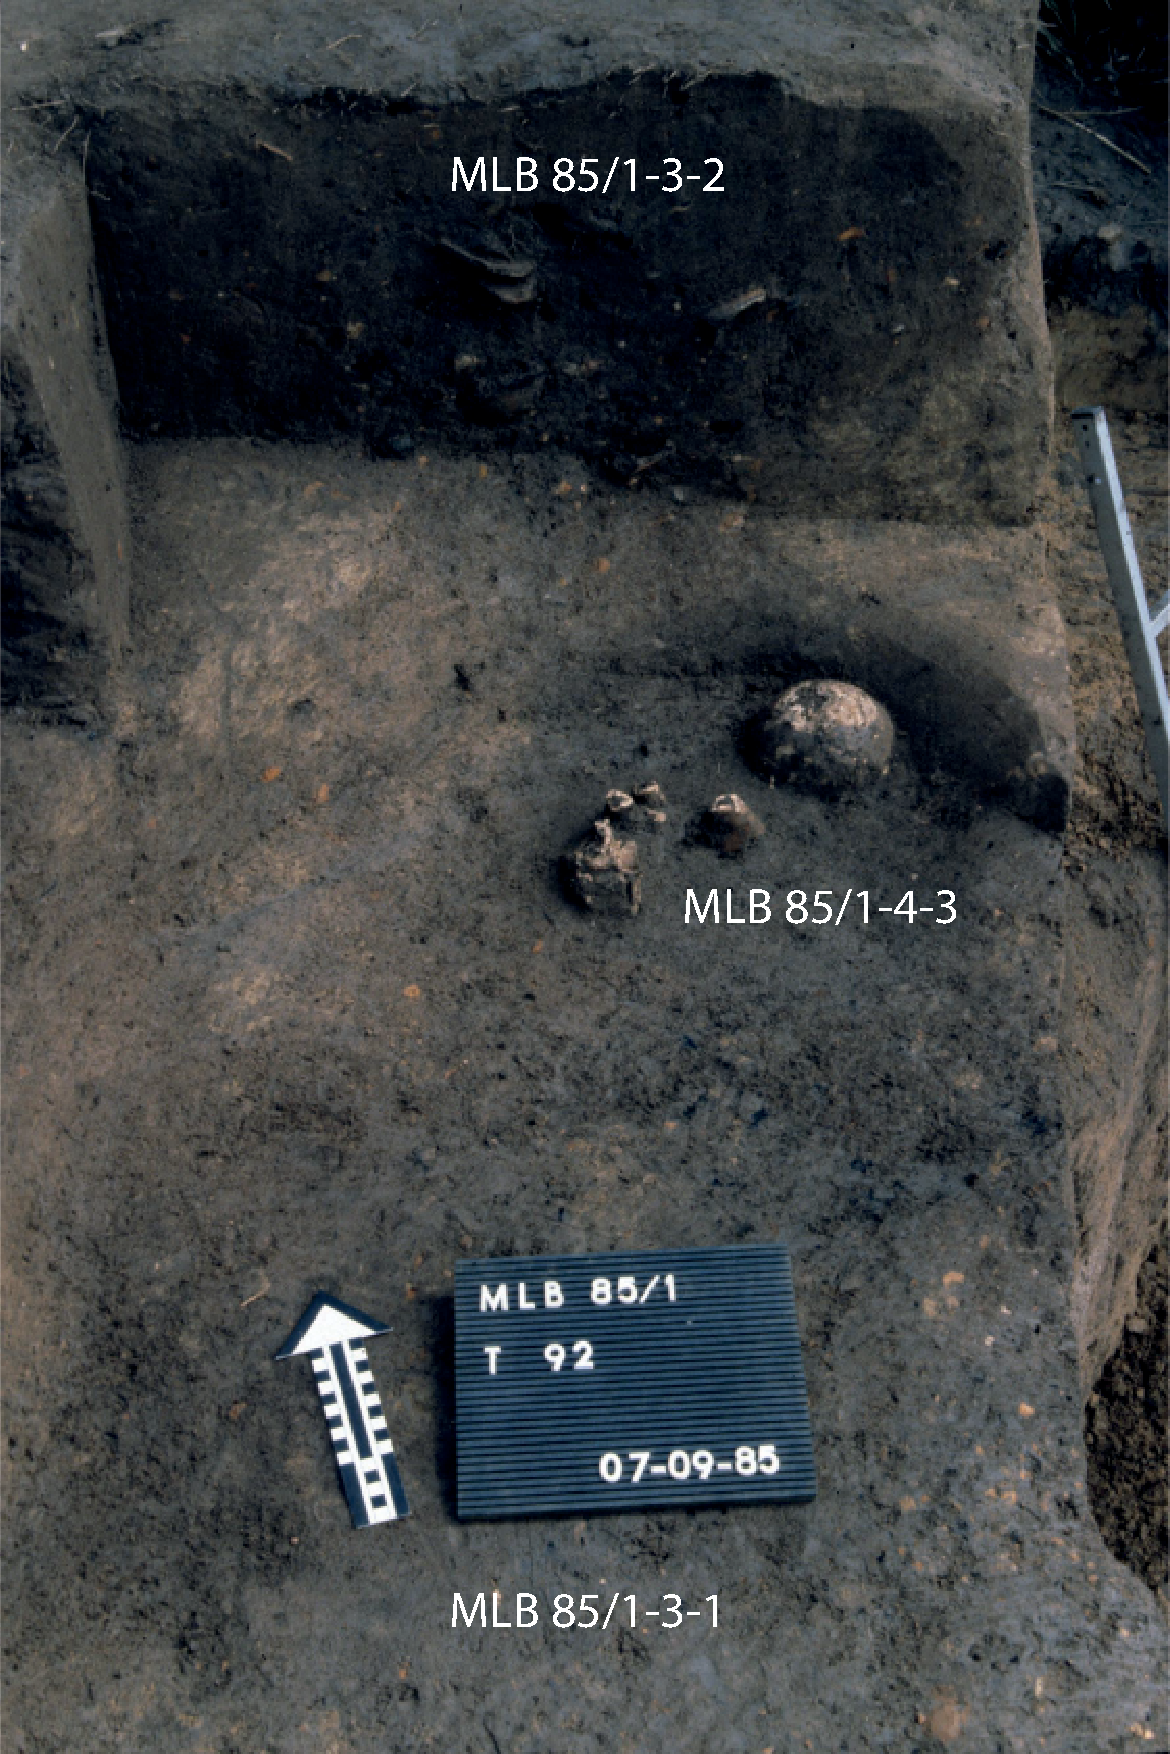
\includegraphics[width=\columnwidth]{fig/MLB85-1_Pl4_E85-031-34.pdf}
 \caption{Planum 4}
 \label{fig:MLB85-1_Pl4}
 \end{subfigure}\hfill
 \begin{subfigure}{\columnwidth}
 \centering
 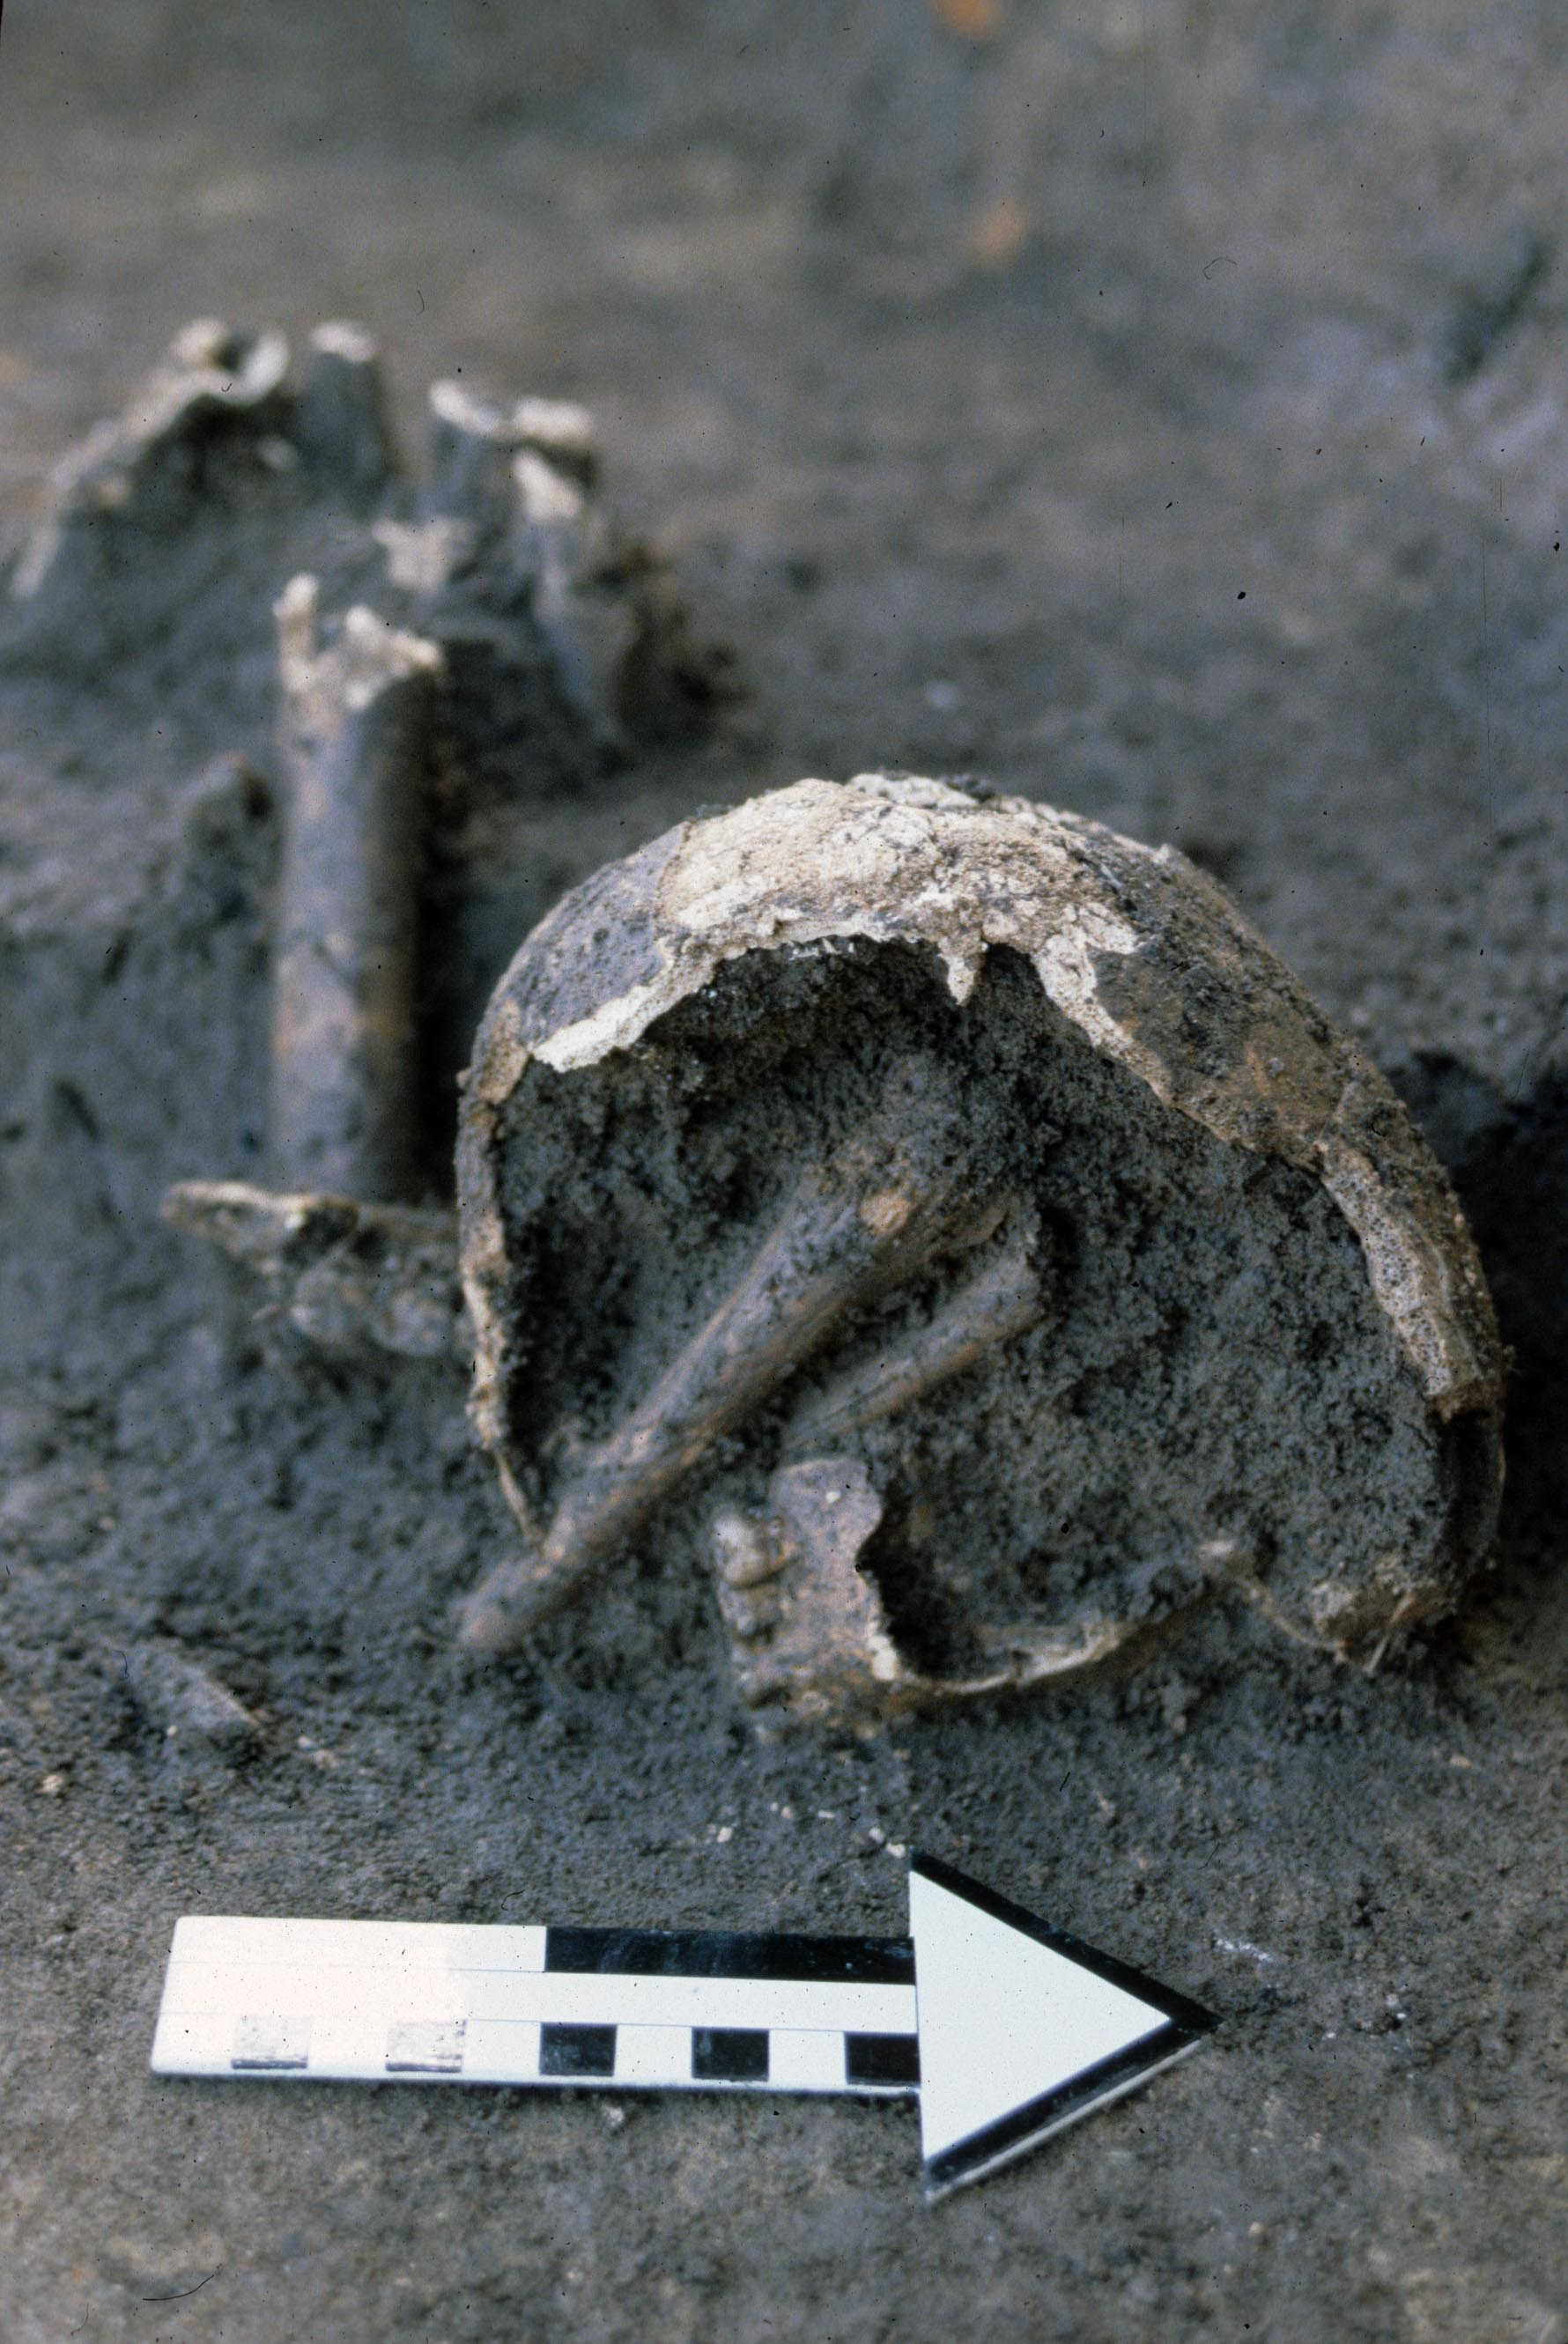
\includegraphics[width=\columnwidth]{fig/MLB85-143_E85-032-10.jpg}
 \caption{Detail}
 \label{fig:MLB85-143_Detail}
 \end{subfigure}
 \caption{MLB 85/1-4-3: a) Planum 4 von Schnitt MLB 85/1 (T 92, Blick von Süden); b) Detail des Schädels (Blick von Osten; Fotos: M. K. H. Eggert, 1985).}
 \label{fig:MLB85-1_SekBest_Fotos}
\end{figure*}

\begin{figure*}[p]
\centering
\begin{subfigure}[b]{\textwidth}
\adjustbox{trim = 0 0 0 {.05\height}, clip}{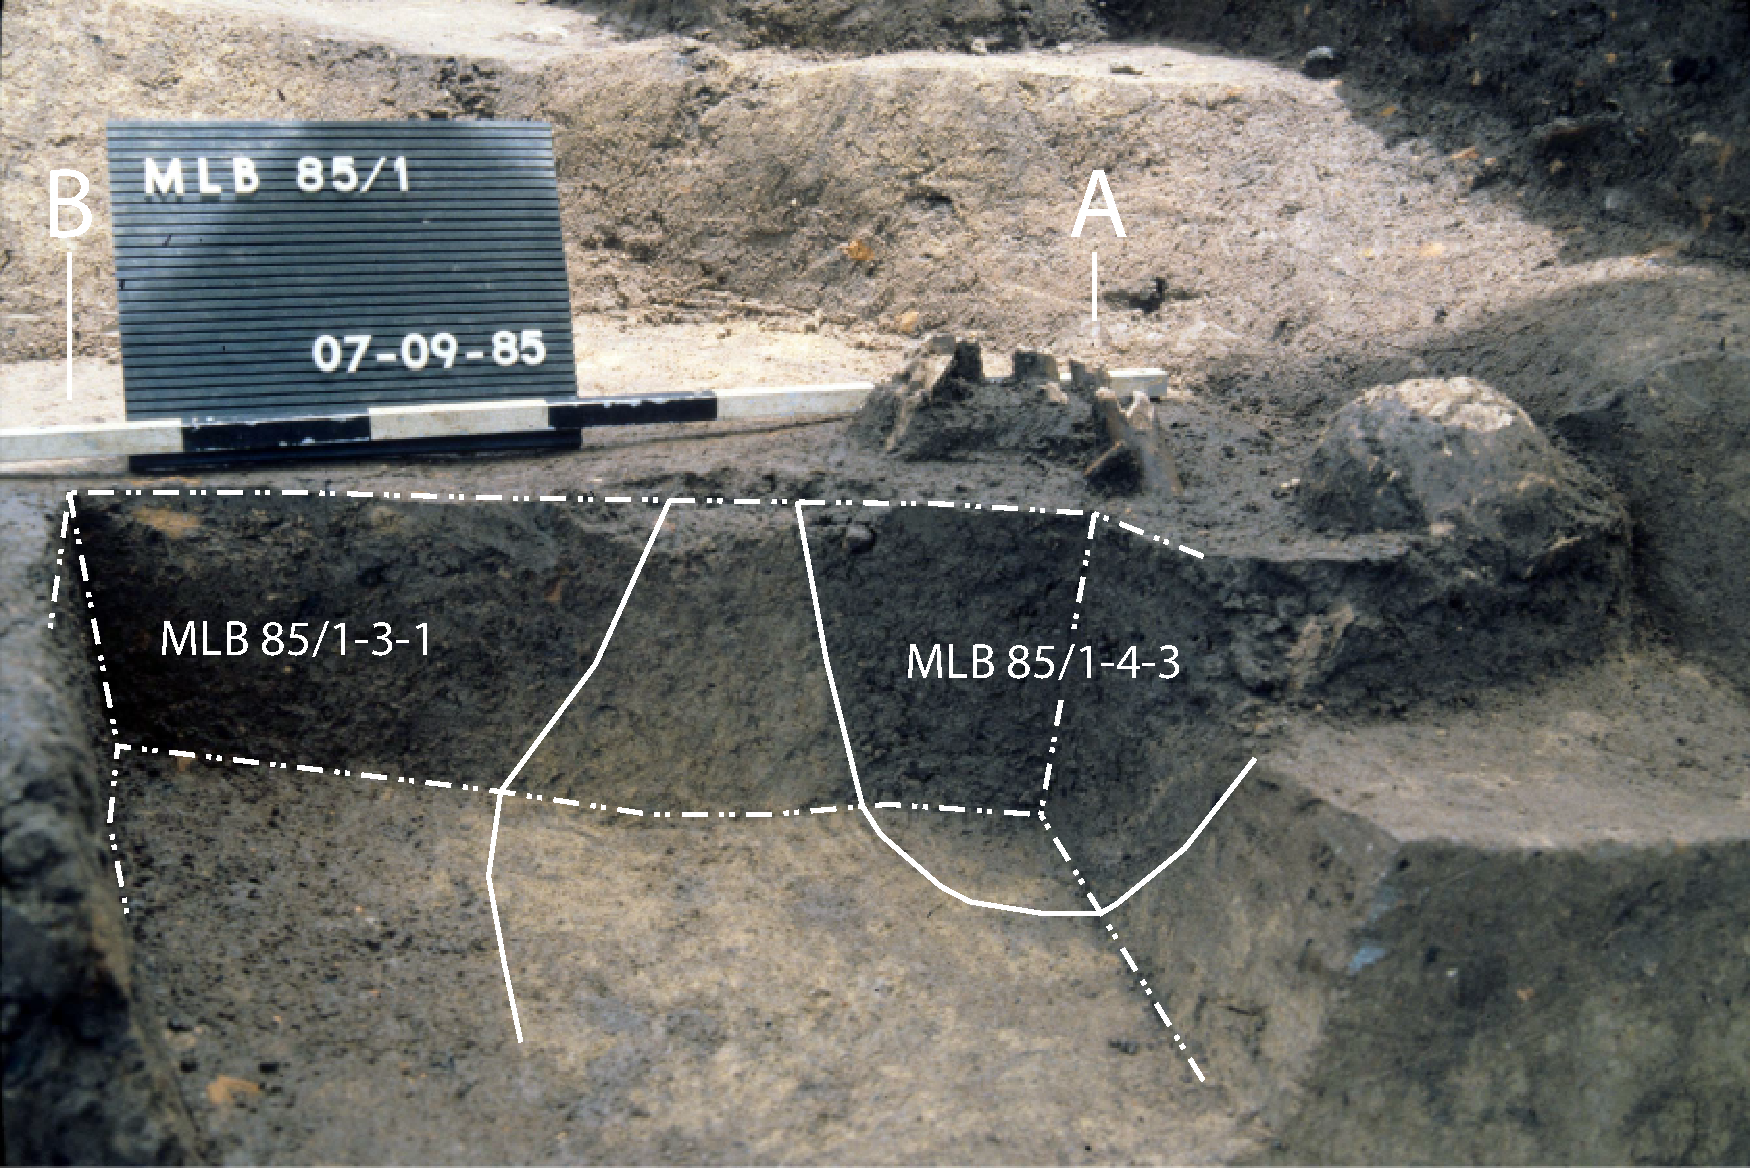
\includegraphics[width = \textwidth]{fig/MLB85-143_E85-032-05.pdf}}
\caption{Profil A--B, Blick von Südosten}
 \label{fig:MLB85-143_Prof_A-B}
 \vspace{1ex}
\end{subfigure}
\begin{subfigure}[b]{\columnwidth}
\includegraphics[width = \columnwidth]{fig/MLB85-143_E85-032-19.pdf}
\caption{Blick von Süden aus Profil E--F}
 \label{fig:MLB85-143_Prof_E-F_1}
\end{subfigure}\hfill
\begin{subfigure}[b]{\columnwidth}
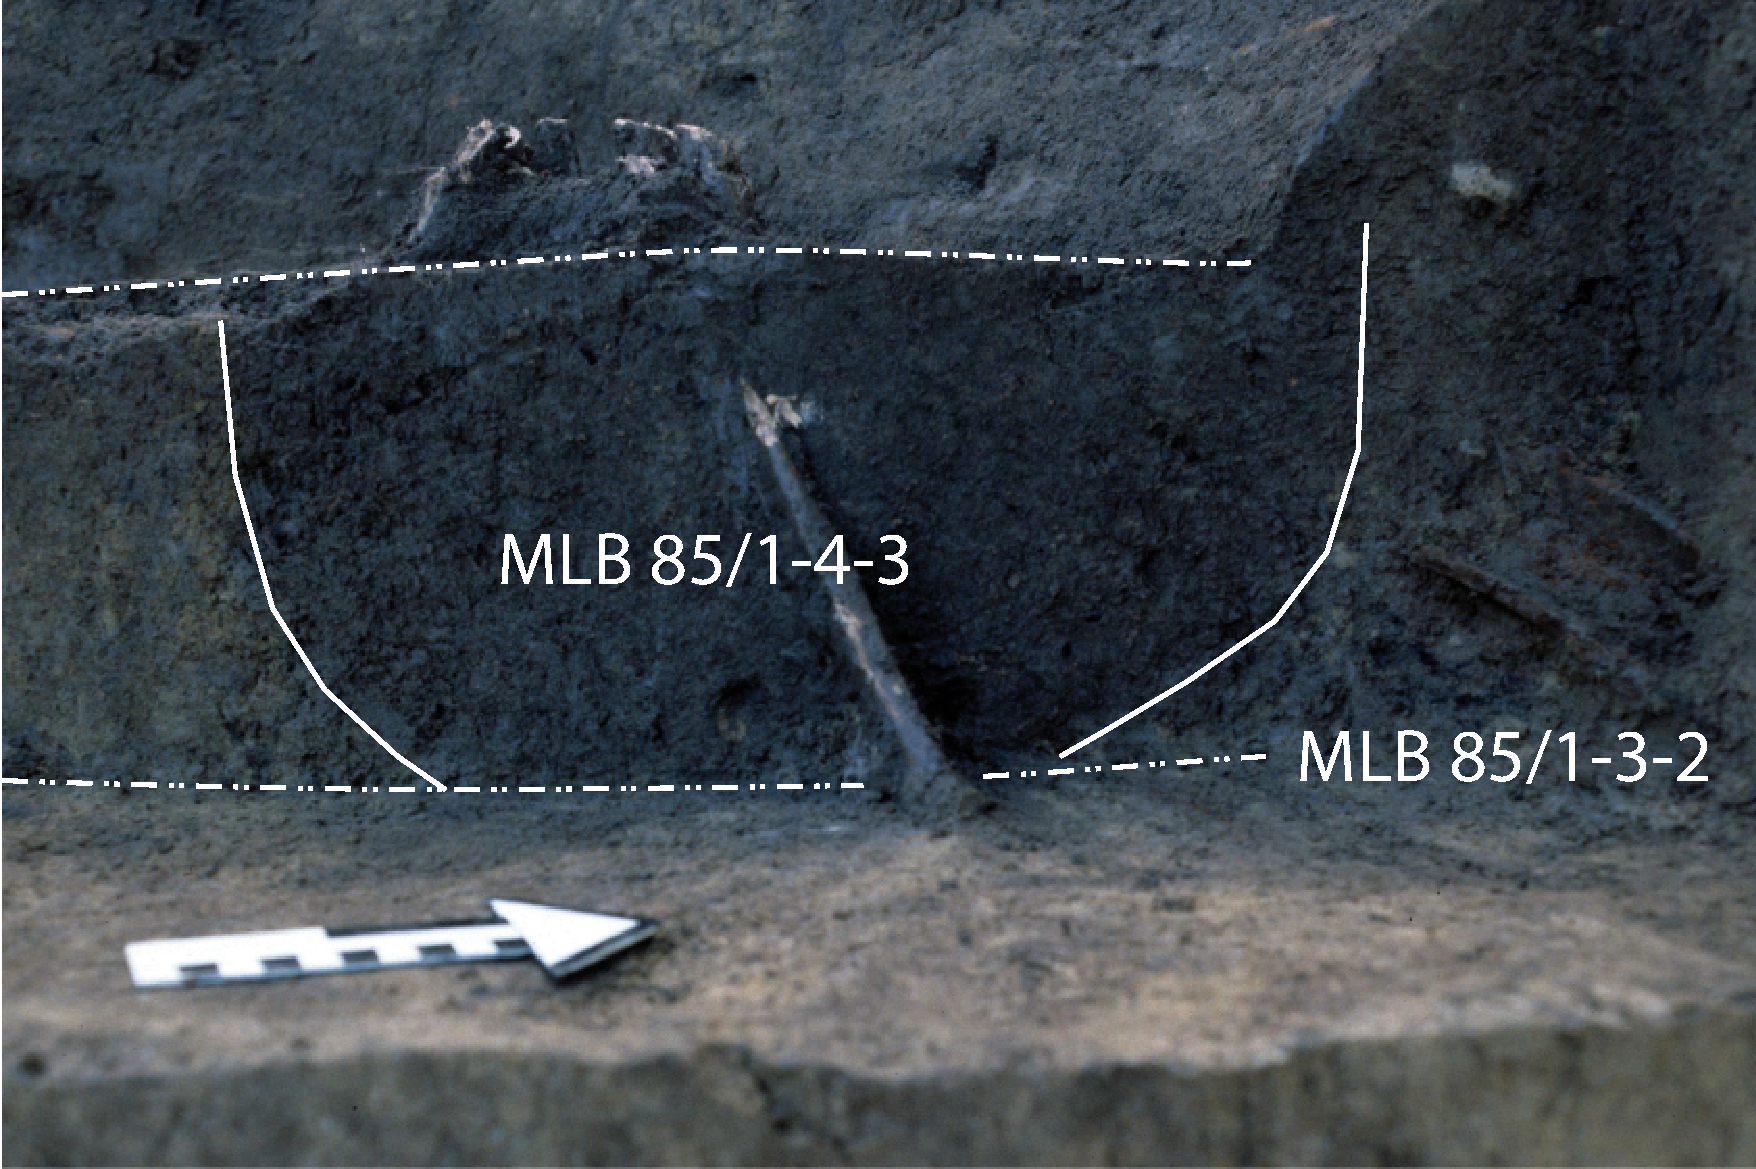
\includegraphics[width = \columnwidth]{fig/MLB85-143_E85-032-16.pdf}
\caption{Profil E--F, Blick von Ostsüdosten}
 \label{fig:MLB85-143_Prof_E-F_2}
\vspace{4.25ex}
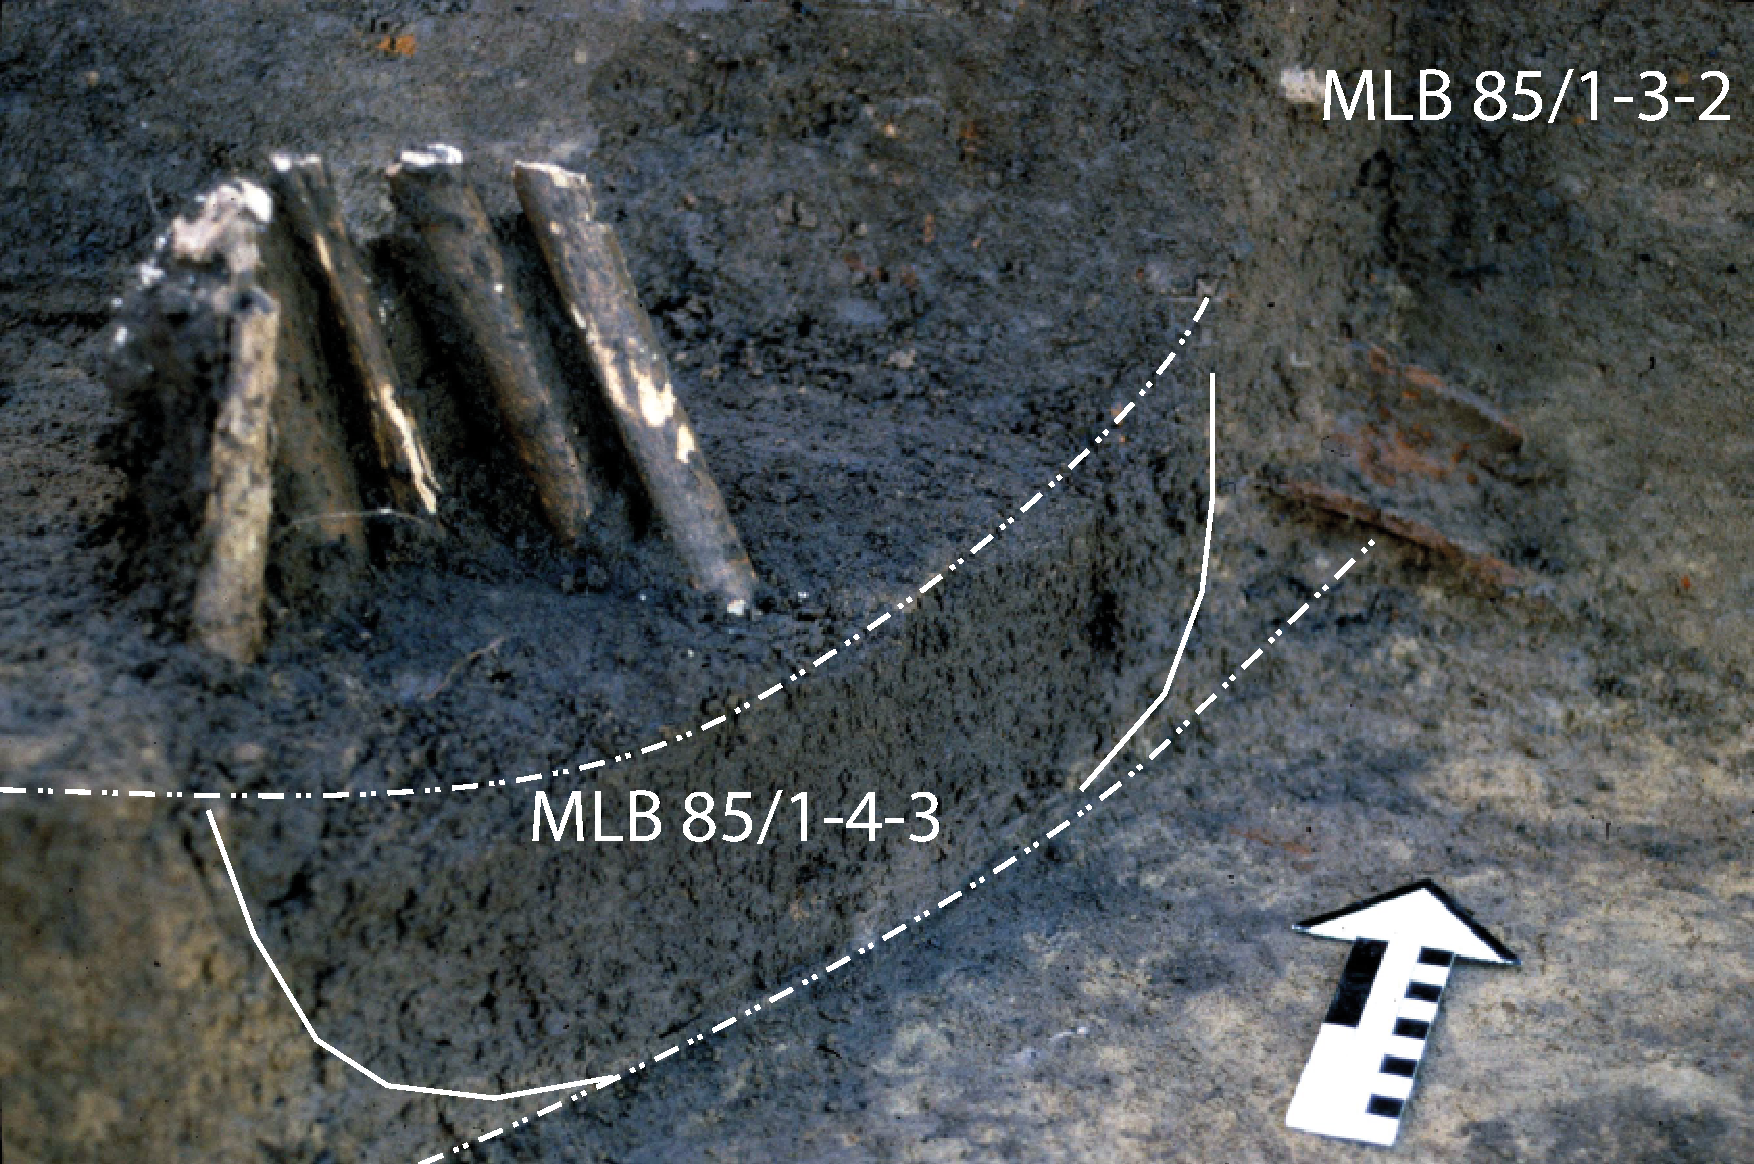
\includegraphics[width = \columnwidth]{fig/MLB85-143_E85-032-22.pdf}
\caption{Zurückverlegtes Profil E--F, Blick von SSO}
 \label{fig:MLB85-143_Prof_E-F_3}
\end{subfigure}
 \caption{MLB 85/1-4-3: Zurückverlegtes Profil E–F (siehe Abb.~\ref{fig:MLB85_1_Zeichnung}), welches die stratigrafische Überlagerung der nördlichen Grube MLB 85/1-3-2 durch die Sekundärbestattung zeigt  (Fotos: M. K. H. Eggert, 1985).}
 \label{fig:MLB85-143}
\end{figure*}

\section*{\begin{tabular*}{\linewidth}{@{}l @{\extracolsep{\fill}} r@{}}
		Nr.~3 & MLB~85/1-4-3\\
	\end{tabular*} 
}

\textsf{\textbf{Maluba (Lua; Fpl.~230)}}

\vspace{1em}

\noindent\begin{tabular}{@{}rl@{}}
	\textbf{Feldarbeit:} & \textbf{05.09.--07.09.1985 (F. Nikulka)} \\ 
	\textbf{Abb.:} & \textbf{\ref{fig:MLB85-1_SekBest_Fotos}--\ref{fig:MLB85-1_SekBest_Skelettbild}} \\
	\textbf{Tab.:} & \textbf{\ref{tab:MLB85_1-4-3_Zaehne}--\ref{tab:MLB85_1-4-3_14C}}\\
	\textbf{Taf.:} & \textbf{27.9} \\ 
	\textbf{Lit.:} & \textbf{\textsc{Eggert}~1987b} \\ 
\end{tabular}

\paragraph{Grabung und Befunde}\hspace{-.5em}|\hspace{.5em}%
In einer nur etwa 0,3\,$\times$\,0,3\,m großen Grube mit schräger Wandung, gerundeten Ecken und konvexer Basis im nördlichen Bereich des Befunds MLB~85/1-3-1 (Kat.-Nr.~1) fanden sich menschliche Skelettreste. Der Befund zeichnete sich bereits im dritten Abtrag ab und wurde im vierten Abtrag deutlich sichtbar (Abb.~\ref{fig:MLB85_1_PlanaT70+90_Foto}). Im auf dem großen Hinterhauptsloch (\textit{Foramen magnum}) liegenden Schädel steckten zwei lange Röhrenknochen, die nicht mehr genauer identifiziert werden können. \textit{Maxilla} und \textit{Mandibula} waren ebenfalls in den Schädel gedrückt. Etwa 15\,cm südwestlich des Schädels waren fünf große Röhrenknochen senkrecht in einem Halbrund dicht nebeneinander an der Wandung der kleinen Grube platziert (Abb.~\ref{fig:MLB85-1_SekBest_Fotos}).

Die Eingrabung ließ sich durch ein Querprofil deutlich erfassen (Abb.~\ref{fig:MLB85-143_Prof_A-B}; siehe auch Abb.~\ref{fig:MLB85_1_Zeichnung}: A--B--C--D). Die stratigraphische Relation zwischen der Sekundärbestattung und der Grube MLB~85/1-3-1 konnte jedoch nicht geklärt werden. Es zeigte sich aber, dass der Befund in die nördlich angrenzende Grube MLB~85/1-3-2 einschneidet (Kat.-Nr.~2; Abb.~\ref{fig:MLB85-143_Prof_E-F_2}).

\begin{figure*}[p]
	\begin{minipage}[b]{.4\textwidth}
 		\caption{MLB 85/1-4-3: Erhaltene Skelettelemente (schwarz: vorhanden, grau: fragmentiert vorhanden und durch Fotos belegt).}\label{fig:MLB85-1_SekBest_Skelettbild}
	\end{minipage}\hfill
	\begin{minipage}[b]{.55\textwidth}
 		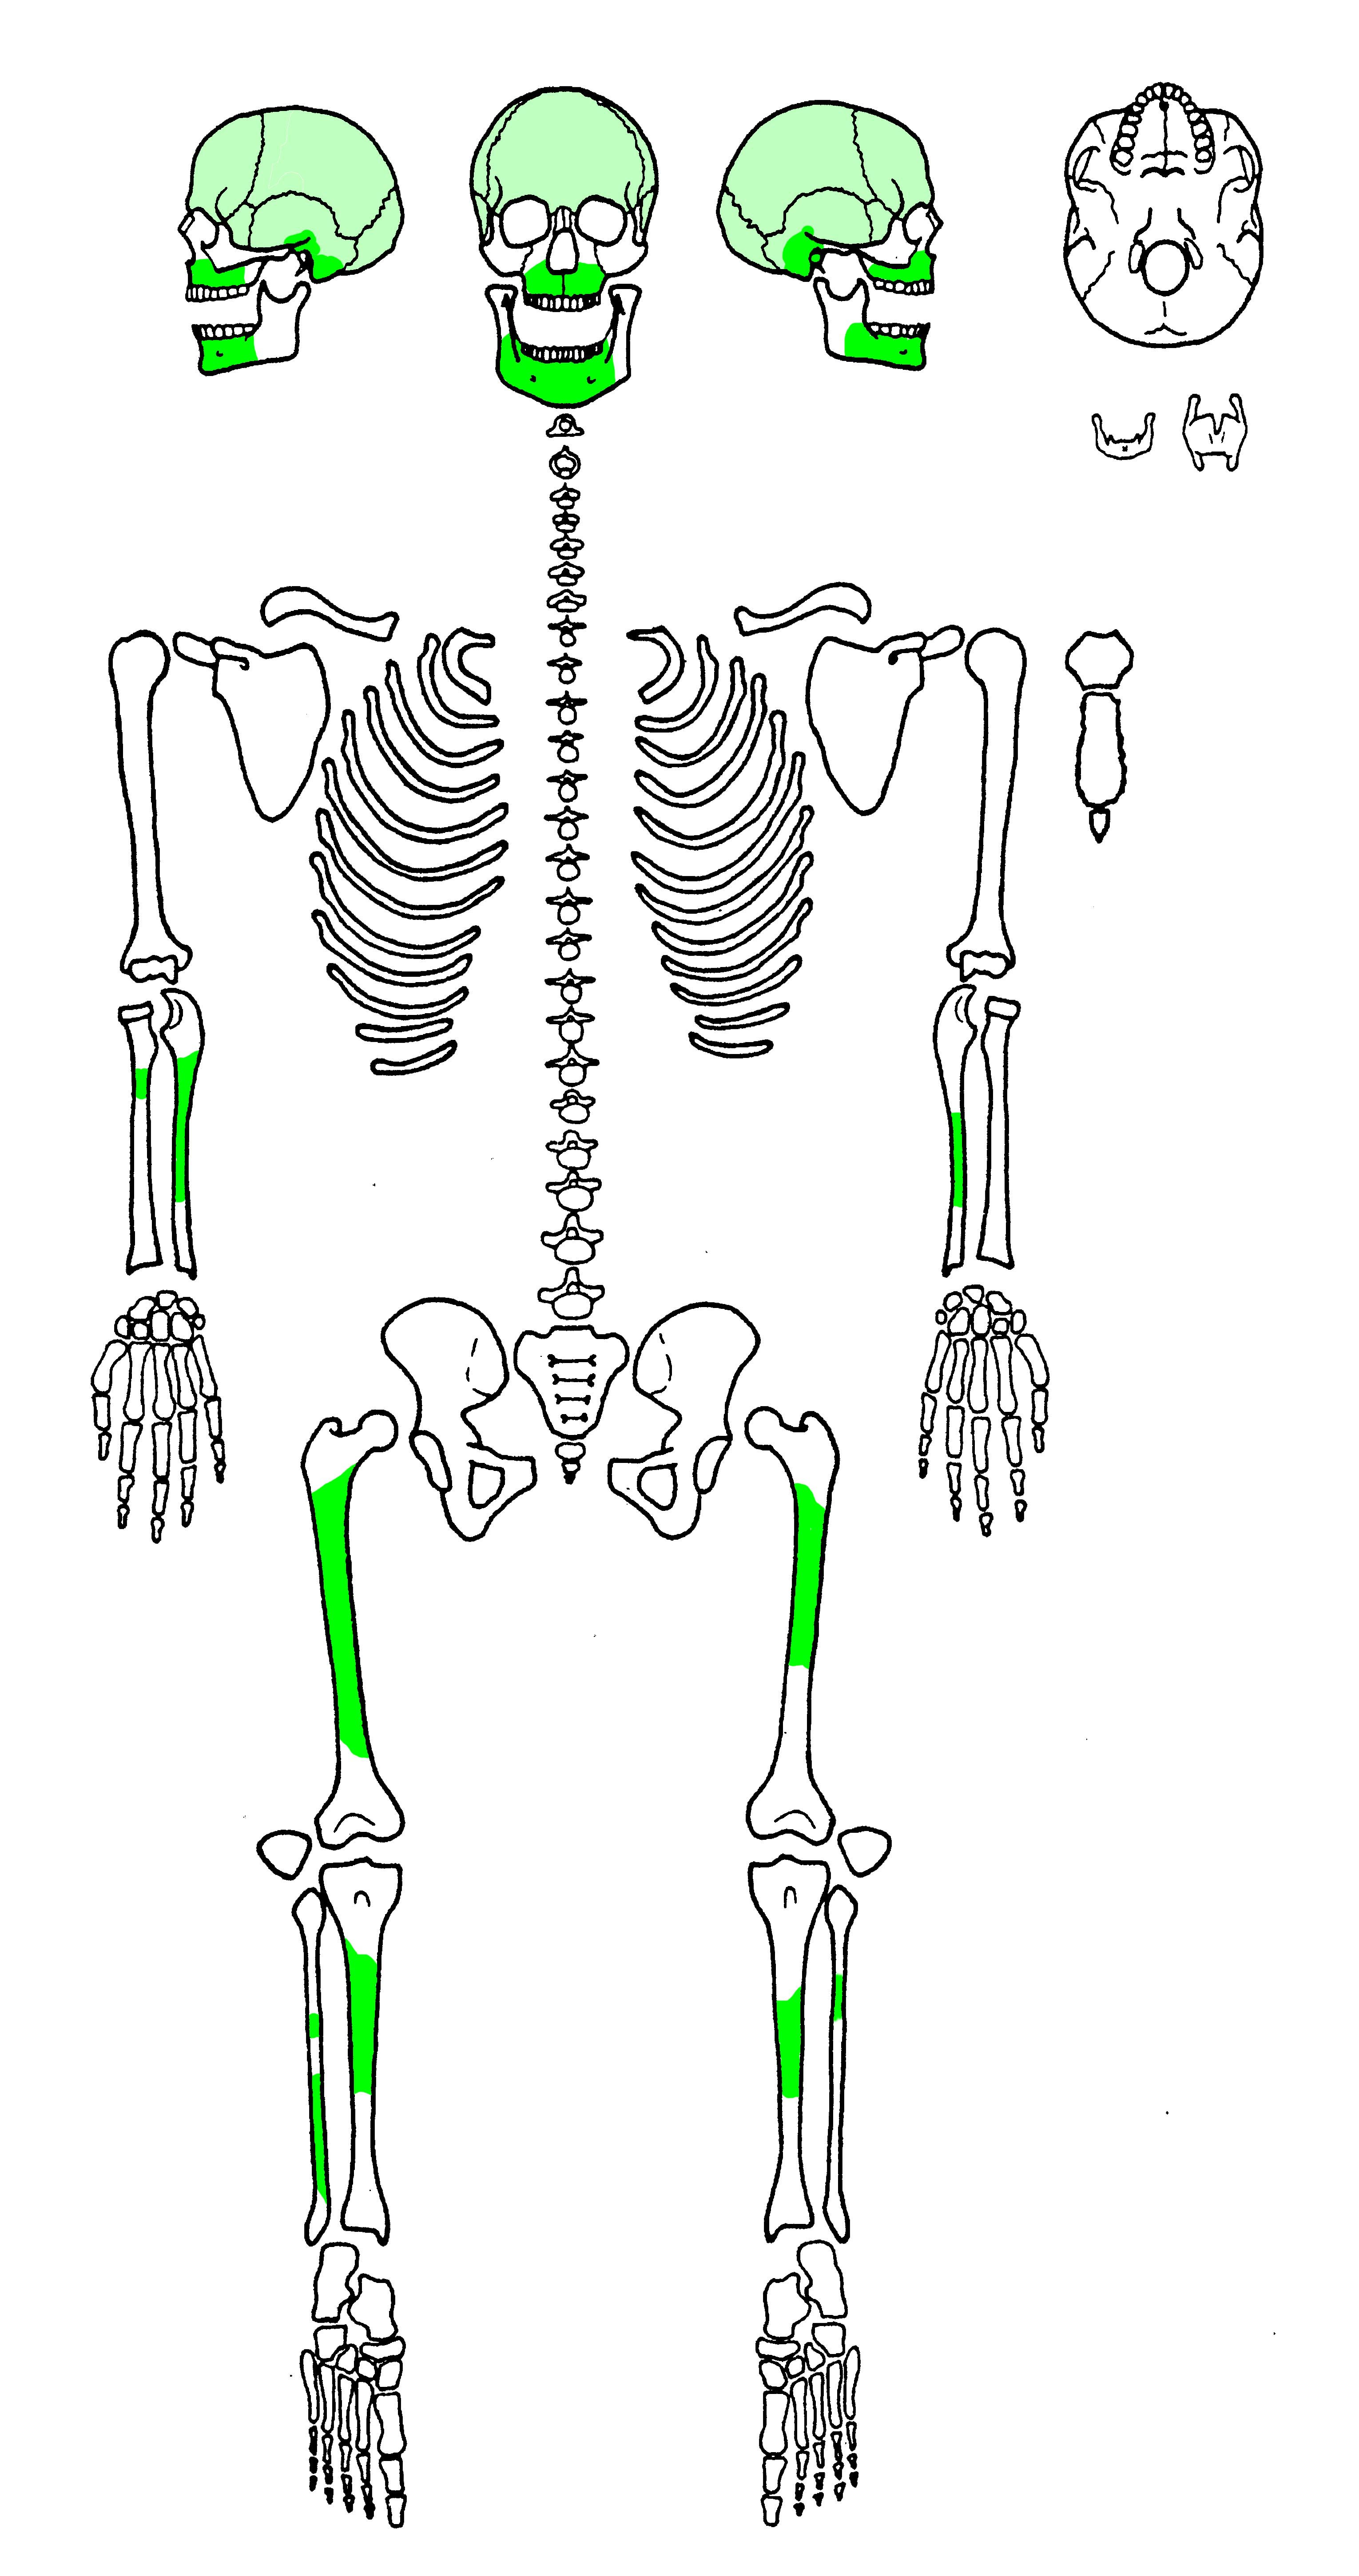
\includegraphics[width=\textwidth]{fig/MLB85-143_Skelettbild_2013-11-09.jpg}
	\end{minipage}
\end{figure*}

\begin{table*}[p]
	\centering
		{\footnotesize
			\begin{sftabular}{@{}cccccccccccccccc@{}}
				\toprule 
				M3 & M2 & M1 & P2 & P1 & C & I2 & I1 & I1 & I2 & C & P1 & P2 & M1 & M2 & M3 \\ 
				18 & 17 & 16 & 15 & 14 & 13 & 12 & 11 & 21 & 22 & 23 & 24 & 25 & 26 & 27 & 28 \\ 
				\midrule 
				$\bullet$ & $\bullet$ & $\bullet$ & $\bullet$ & $\bullet$ & $\bullet$ & $\star$ & $\star$ & - & - & $\bullet$ & $\bullet$ & $\bullet$ & $\bullet$ & $\bullet$ & $\circ$ \\ 
				$\star$ & $\circ$ & $\circ$ & $\star$ & $\bullet$ & $\bullet$ & $\star$ & $\star$ & - & - & $\bullet$ & $\bullet$ & $\star$ & $\circ$ & $\circ$ & $\star$ \\ 
				\midrule
				48 & 47 & 46 & 45 & 44 & 43 & 42 & 41 & 31 & 32 & 33 & 34 & 35 & 36 & 37 & 38 \\ 
				\bottomrule
		\end{sftabular}}
	\caption{MLB 85/1-4-3: Zähne ($\bullet$ = vorhanden, $\star$ = Wurzel vorhanden, Krone fehlt, $\circ$ = Krone lose vorhanden) -- (Ansicht: rechts – links).}
	\label{tab:MLB85_1-4-3_Zaehne}
\end{table*}

\begin{table*}[p]
\centering
		{\footnotesize \begin{sftabular}{@{}cccccc@{}}
				\toprule 
				M3 & M2 & M1 & M1 & M2 & M3 \\ 
				18 & 17 & 16 & 26 & 27 & 28 \\ 
				\midrule 
				2 & 3+ -- 4 & 5 -- 5+ & 5 -- 5+ & 4 & 2 -- 2+ \\ 
				- & 2 & 3 -- 3+ & 3 -- 3+ & 2 & - \\ 
				\midrule 
				48 & 47 & 46 & 36 & 37 & 38 \\ 
				\bottomrule 
		\end{sftabular}}
	\caption{MLB 85/1-4-3: Abrasionsgrad der Molaren nach \textcite[72 Abb.~3.9]{Brothwell.1981}.}
	\label{tab:MLB85_1-4-3_ZaehneAbrasion}
\end{table*}

\paragraph{Anthropologie}\hspace{-.5em}|\hspace{.5em}%
Die Knochen wurden 1986 durch P. Caselitz (Hamburg) begutachtet (\textsc{Caselitz} 1986) und im Appendix des die Feldarbeiten von 1985 entlang des \mbox{Ubangi} beschreibenden Aufsatzes von \textcite[144]{Eggert.1987c} kurz beschrieben.\footnote{Im Jahr 2013 erfolgte eine erneute Begutachtung und Beschreibung des Materials durch den Autor. Für die Diskussion zu dieser Bestimmungen danke ich Michael Francken (Tübingen).}

Das Inventar umfasst viele Bruchstücke des Hirnschädels (\textit{Neurocranium}), der auf den 1985 gemachten Grabungsfotos noch teilweise erhalten war (Abb.~\ref{fig:MLB85-1_SekBest_Skelettbild}), 2013 aber nur noch in stark fragmentiertem Zustand vorlag. Es fanden sich kaum Teile größer als 5\,$\times$\,5\,cm. Alle Fragmente weisen regelhaft sehr verrundete Bruchkanten auf. Die Oberflächen der Knochenfragmente sind stark angelöst. An zwei Bruchstücken sind \textit{endocranial} noch Nahtbereiche sichtbar, jedoch lässt sich nicht bestimmen, um welchen Nahtbereich es sich handelt. Vom Gesichtsschädel (\textit{Viscoerocranium}) waren nur sehr wenige, noch stärker fragmentierte Teile erhalten.

Ober- (\textit{Maxilla}) und Unterkiefer (\textit{Mandibula}) sind deutlich besser erhalten und liegen fast vollständig vor. Vom \textit{Ramus mandibulae} ist auf der rechten Seite jedoch nur der Ansatz vorhanden, links fehlt er völlig. Der Unterkiefer ist generell sehr robust. Im Oberkiefer liegt eine deutliche Prognathie im Bereich der Schneidezähne (\textit{Incisivi}) vor. Die beiden \textit{Incisivi} der linken Seite fehlen im Ober- wie im Unterkiefer komplett (Tab. \ref{tab:MLB85_1-4-3_Zaehne}). Von insgesamt acht Zähnen fehlen die Kronen und nur die Wurzeln sind erhalten. Bei einigen \textit{Molaren} liegen die Kronen separat vor, können aufgrund der Fragmentierung der zugehörigen Wurzeln aber nicht mehr angepasst werden. Die Zähne weisen eine deutliche Abrasion auf (Tab. \ref{tab:MLB85_1-4-3_ZaehneAbrasion}). Deutlich sichtbare Zahnengstellen zeigen sich zwischen dem zweiten \textit{Incisivus} (42) und dem \textit{Caninus} (43) im Unterkiefer auf der rechten Seite. Der zweite \textit{Incisivus} im Oberkiefer links (22) weist buccal einen möglichen Wurzelabszess mit Eröffnung des Knochens an der Wurzelspitze auf (\textsc{Caselitz} 1986). Der dritte \textit{Molar} im Oberkiefer links (28) ist in die Nasennebenhöhle durchgebrochen. Die \textit{Canini} und \textit{Prämolaren} im Unterkiefer zeigen Zahnsteinanlagerungen und fast alle Wurzeltaschen sind parodontitisch (\textsc{Caselitz} 1986). Die Abrasion der Kauflächen ist nicht besonders stark. Das Dentin ist nur an einigen Stellen sichtbar.

Von den Wirbeln ist lediglich der \textit{Arcus anterior} des Atlas mit der \textit{Fovea dentis} erhalten (\textsc{Caselitz} 1986). Das postcraniale Skelettmaterial besteht aus Diaphysenfragmenten der oberen und unteren Extremitäten. Epiphysenfragmente konnten nicht beobachtet werden. Es handelt sich um Reste beider \textit{Femora}, \textit{Tibie}, \textit{Fibulae}, \textit{Ulnae} sowie des rechten \textit{Radius} (Abb.~\ref{fig:MLB85-1_SekBest_Skelettbild}). Die Knochen machen allgemein einen eher grazilen Eindruck. Es lassen sich keine pathologischen Auffälligkeiten beobachten.\footnote{Maße, die beispielsweise für eine Körperhöhenrekonstruktion genutzt werden könnten, konnten aufgrund der Unvollständigkeit nicht abgenommen werden.} Zwischen den Knochen der rechten und linken Körperhälfte konnten keine Unterschiede beobachtet werden, somit kann davon ausgegangen werden, dass die \textit{endocranialen} Skelettteile von einem Individuum stammen. Die generelle Robustizität des Knochenmaterials legt den Schluss nahe, dass \textit{craniales} und \textit{endocraniales} Material zusammengehören und somit eine Auswahl der Skelettteile eines Individuums vorliegen.

\begin{table*}[!tb]
	\centering
	{\footnotesize \begin{sftabular}{@{}p{.125\textwidth}p{.15\textwidth}p{.4\textwidth}p{.2\textwidth}@{}}
			\toprule 
			\textbf{Lab-Nr} & \textbf{Datum (bp)} & \textbf{Datum (2-Sigma)} & \textbf{Probe }\\ 
			\midrule 
			Poz-62102 & 580 \( \pm \) 30 & \begin{tabular}[t]{@{}l@{}}1300--1369 n.~Chr. (63,6\,\%)\\ 1381--1419 n.~Chr. (31,8\,\%)\end{tabular} & Fibula \\ 
			Poz-62103 & 810 \( \pm \) 80 & 1030--1297 n.~Chr. & Ulna \\ 
			\bottomrule 
	\end{sftabular} }
	\caption{MLB 85/1-4-3: \textsuperscript{14}C-Datierungen.}
	\label{tab:MLB85_1-4-3_14C}
\end{table*}

Der Zahnbefund, mit den dritten \textit{Moralen} in der Kauebene und bereits leichter Abrasion, weist auf ein mindestens adultes Sterbealter des Individuums hin.\footnote{Angaben zu Alter und Geschlecht können ohne Kenntnis der Populationsvarianz nur grobe Schätzungen sein. Die hier gemachten Angaben sind nur als grobe Deutung beziehungsweise Ansprache der beobachteten Merkmale zu sehen.} Die Zahnkronenabrasion nach \textcite[72~Fig.~3.9]{Brothwell.1981} ergibt ein Sterbealter von 25--35, eventuell auch 35--45 Jahren.\footnote{Es muss an dieser Stelle auf das Fehlen von Vergleichen für zentralafrikanische Populationen hingewiesen werden. Da die Zahnkronenabrasion zentral von der konsumierten Nahrung abhängt, können die von \textcite{Brothwell.1981} gemachten Angaben nur einen groben Richtwert liefern.} Im Bereich des Nahtverschlusses des harten Gaumens ist lediglich der distale Bereich der AMP-Sutura und der Bereich der IN-Suturen erhalten, während der Bereich der TP-Naht zu fragmentarisch erhalten ist \parencites[siehe][]{Mann.1987}[782 Abb.~1]{Mann.1991}{Apostolidou.2011}. Dass die IMP-Naht nicht verstrichen, die IN-Naht hingegen verstrichen ist, deutet nach \textcite[783 Tab 1, Abb. 2]{Mann.1991} auf ein Sterbealter zwischen 20--25 und 50\textsuperscript{+} Jahren hin. Der \textit{endocraniale} Nahtverschluss, mit den teilweise noch sichtbaren Nähten unterstreicht diesen (spät)adulten bis maturen Befund. Ein Problem bereitet jedoch die Tatsache, dass sich keine Aussage bezüglich des Nahtbereiches, aus dem die Fragmente stammen, treffen lässt. Alles in allem deuten die beobachtbaren Merkmale auf ein tendenziell spätadultes Sterbealter, zwischen 25--45 Jahren hin.

Das nicht ausgeprägte Kinn kann als weibliches Merkmal interpretiert werden, ebenso wie der flache Winkel der \textit{Pars petrosa}.\footnote{Aufgrund der schlechten Erhaltung und fehlender Skelettelemente lässt sich die kombinierte Methode nach \textcite{Ferembach.1979} nicht anwenden. Eine Ansprache des Geschlechts des Individuums lässt sich nur auf Basis von Einzelmerkmalen vornehmen.} Die allgemeine Robustizität, die von Caselitz \parencite[siehe][144]{Eggert.1987c} als Hinweis auf ein männliches Geschlecht angeführt wird, ist bei Personen aus Afrika häufiger zu beobachten\footnote{Mündl. Mitt. M. Francken (2013).} und kann ohne Populationsdaten nur bedingt als Argument herangezogen werden.\footnote{Eine Geschlechtsdifferenzierung auf Basis der \textit{bukko-lingualen} Zahnkronendurchmesser nach \textcite{Alt.1998} wurde versucht. Sie erbrachte jedoch keine verwertbare Aussage, da die Populationsvariabilität unbekannt ist und Vergleichswerte für afrikanische Populationen fehlen. Die Zähne des Skeletts MLB~85/1-4-3 sind 5--40\% größer als die eines Individuums aus dem Befund LBT~98/9 in Lobethal am Sanaga in Südwestkamerun (\textsc{Francken} 2009).} Das Geschlecht des Individuums kann insgesamt nur als unbestimmt mit einer Tendenz zum Weiblichen angesprochen werden.\columnbreak

\paragraph{Keramik\vspace{.5em}}\mbox{}\\
\begin{tabular}{@{}lrl@{}}
	Bearbeitet:	& 76\,g & (100\,\%) \\ 
\end{tabular} 

\vspace{1em}
\noindent Unter dem Komplex MLB~85/1-4-3 sind insgesamt sieben Scherben mit einen Gesamtgewicht von lediglich 76\,g verzeichnet. Es handelt sich dabei größtenteils um Vertreter des Batalimo-Maluba-Stils. Jedoch fanden sich unter den nicht individuell beschrifteten, undiagnostischen Stücken auch Scherben des \textit{Fabrics} 7, welches für die am Fundplatz ebenfalls gefundene Keramik der Matoto-Gruppe charakteristisch ist (Kap.~\ref{sec:MAT-Gr}). In den Abträgen oberhalb des dritten Planums der Grube MLB~85/1-3-1 (Kat.-Nr.~1) wurden die Funde aus dem Bereich über der Sekundärbestattung MLB~85/1-4-3 nicht getrennt. Die in diesen Abträgen gefundene, nicht zur Batalimo-Maluba-Gruppe zugehörige Keramik könnte potenziell im Zuge der Anlage der Sekundärbestattung MLB~85/1-4-3 in Tiefen gelangt sein. Keramik, die potenziell den Stilgruppen Matoto und Bobulu (Kap.~\ref{sec:BBL-Gr}) zugerechnet werden kann, fand sich auch in den Abträgen 4--5 (Abb.~\ref{fig:MLB85-1_KeramikStilgruppen}).\footnote{Die Abträge 4--5 der Grabung MLB~85/1-3-1 wurden auf jener Tiefe angelegt, in der sich auch die Sekundärbestattung MLB~85/1-4-3 fand (Abb.~\ref{fig:MLB85_1_Zeichnung}).} Es kann als wahrscheinlich gelten, dass eben jene Scherben der Stilgruppen Matoto und Bobulu, die in den Abträgen 4 und 5 des Befundes MLB~85/1-3-1 gefunden wurden, im Zusammenhang mit der Anlage der Sekundärbestattung MLB~85/1-4-3 stehen. Die starke Fragmentierung und Mischung von Stilgruppen legt den Schluss nahe, dass das Material nicht als \textit{Beigabe} in den Befund gelangte, sondern lediglich ein Teil der Verfüllung ist.

\paragraph{Datierung}\hspace{-.5em}|\hspace{.5em}%
Zwei Proben von Knochenfragmenten\footnote{Von einem Fragment der Schädelkalotte konnte kein Kohlenstoff mehr extrahiert werden.} aus der Sekundärbestattung MLB~85/1-4-3 wurden im Jahr 2014 radiokohlenstoffdatiert. Eine Probe von der rechten Ulna und eine weitere der rechten Fibula ergaben eine Datierung in das 11.--15.~Jh. n.~Chr. (Abb.~\ref{fig:MLB85_1_14C-Kalibration}, Tab.~\ref{tab:MLB85_1-4-3_14C}).\footnote{Die unkalibrierten Datierungen zeigen innerhalb der zweifachen Standardabweichung keine Überschneidung. Auf Basis dieser Beobachtung könnte davon ausgegangen werden, dass die Knochen nicht im Zuge eines einzelnen Ereignisses deponiert wurden und eine Mehrphasigkeit des Befundes vorliegt. Vor dem Hintergrund der präsentierten archäologischen wie anthropologischen Auswertung ergeben sich jedoch keinerlei Hinweise auf ein solches Szenario. Das anthropologische Material zeigt keine Hinweise für die Repräsentanz mehrerer Individuen und wird die dreifache Standardabweichung zugrunde gelegt, zeigen die unkalibrierten Radiokohlenstoffalter eine Überschneidung von annähernd 100 Jahren.}  

\paragraph{Interpretation}\hspace{-.5em}|\hspace{.5em}%
Unter der Bezeichnung MLB~85/1-4-3 wurde eine -- in einer kleinen Eingrabung deponierte -- Sekundärbestattung eines geschlechtlich unbestimmten, tendenziell weiblichen Individuums, das im Alter von 25--45 Jahren verstorben ist, erfasst. Teile der großen Langknochen wurden aufrecht am Rand der kleinen Grube aufgestellt. Weitere Langknochen wurden in den Schädel gesteckt und dieser dann ebenfalls in der Grube deponiert.\footnote{Die primären Bestattungsriten lassen sich anhand des Befundes ebenso wenig rekonstruieren, wie die Zeit, die zwischen Primär- und Sekundärbestattung lag. Mögliche Vergleiche bieten die von \textcite[266--268]{Wotzka.1993} beschriebenen Bestattungssitten der Fali in Nordkamerun. Diese beinhalten eine Entnahme des Schädels des Verstorbenen aus der primären Grabgrube nach drei Jahren und erneute Bestattung in einem Gefäß an einem anderen Ort \parencite[268]{Wotzka.1993}.} Zwei an Knochenmaterial datierte Radiokohlenstoffproben stellen den Befund in das 11.--15.~Jh. n.~Chr. Die Datierungen aus der Bestattung stellen einen \textit{terminus post quem} für die Datierung der in der Verfüllung angetroffenen Matoto-Keramik dar (Kap.~\ref{sec:MAT-Gr}).

\begin{figure*}[tb]
	\noindent\begin{minipage}[b]{\columnwidth}
		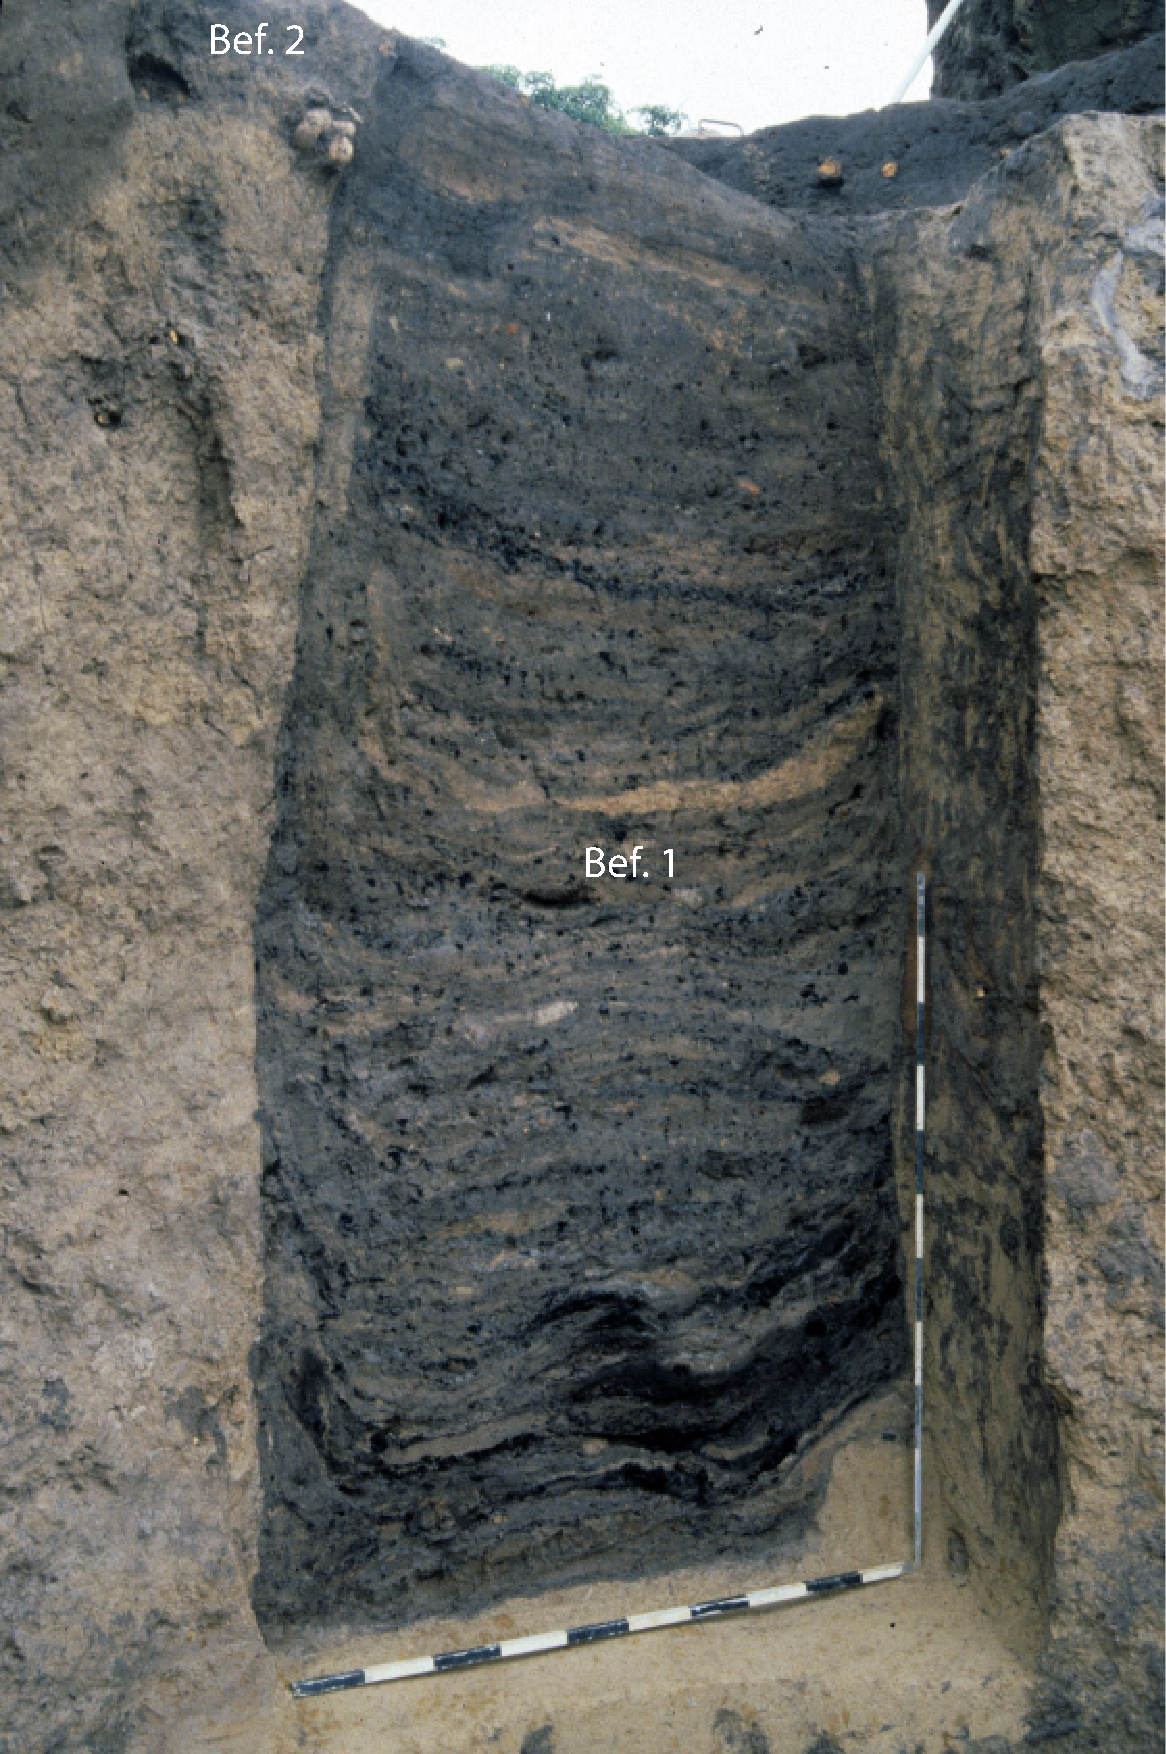
\includegraphics[width=\columnwidth]{fig/MLB85-2_Profil_E85-031-4.pdf}
		\captionof{figure}{MLB~85/2: Zurückverlegtes und geputztes Profil (Foto: M. K. H. Eggert, 1985).\label{fig:MLB85-2_Prof_geputzt}}
	\end{minipage}\hfill
	\noindent\begin{minipage}[b]{\columnwidth}
		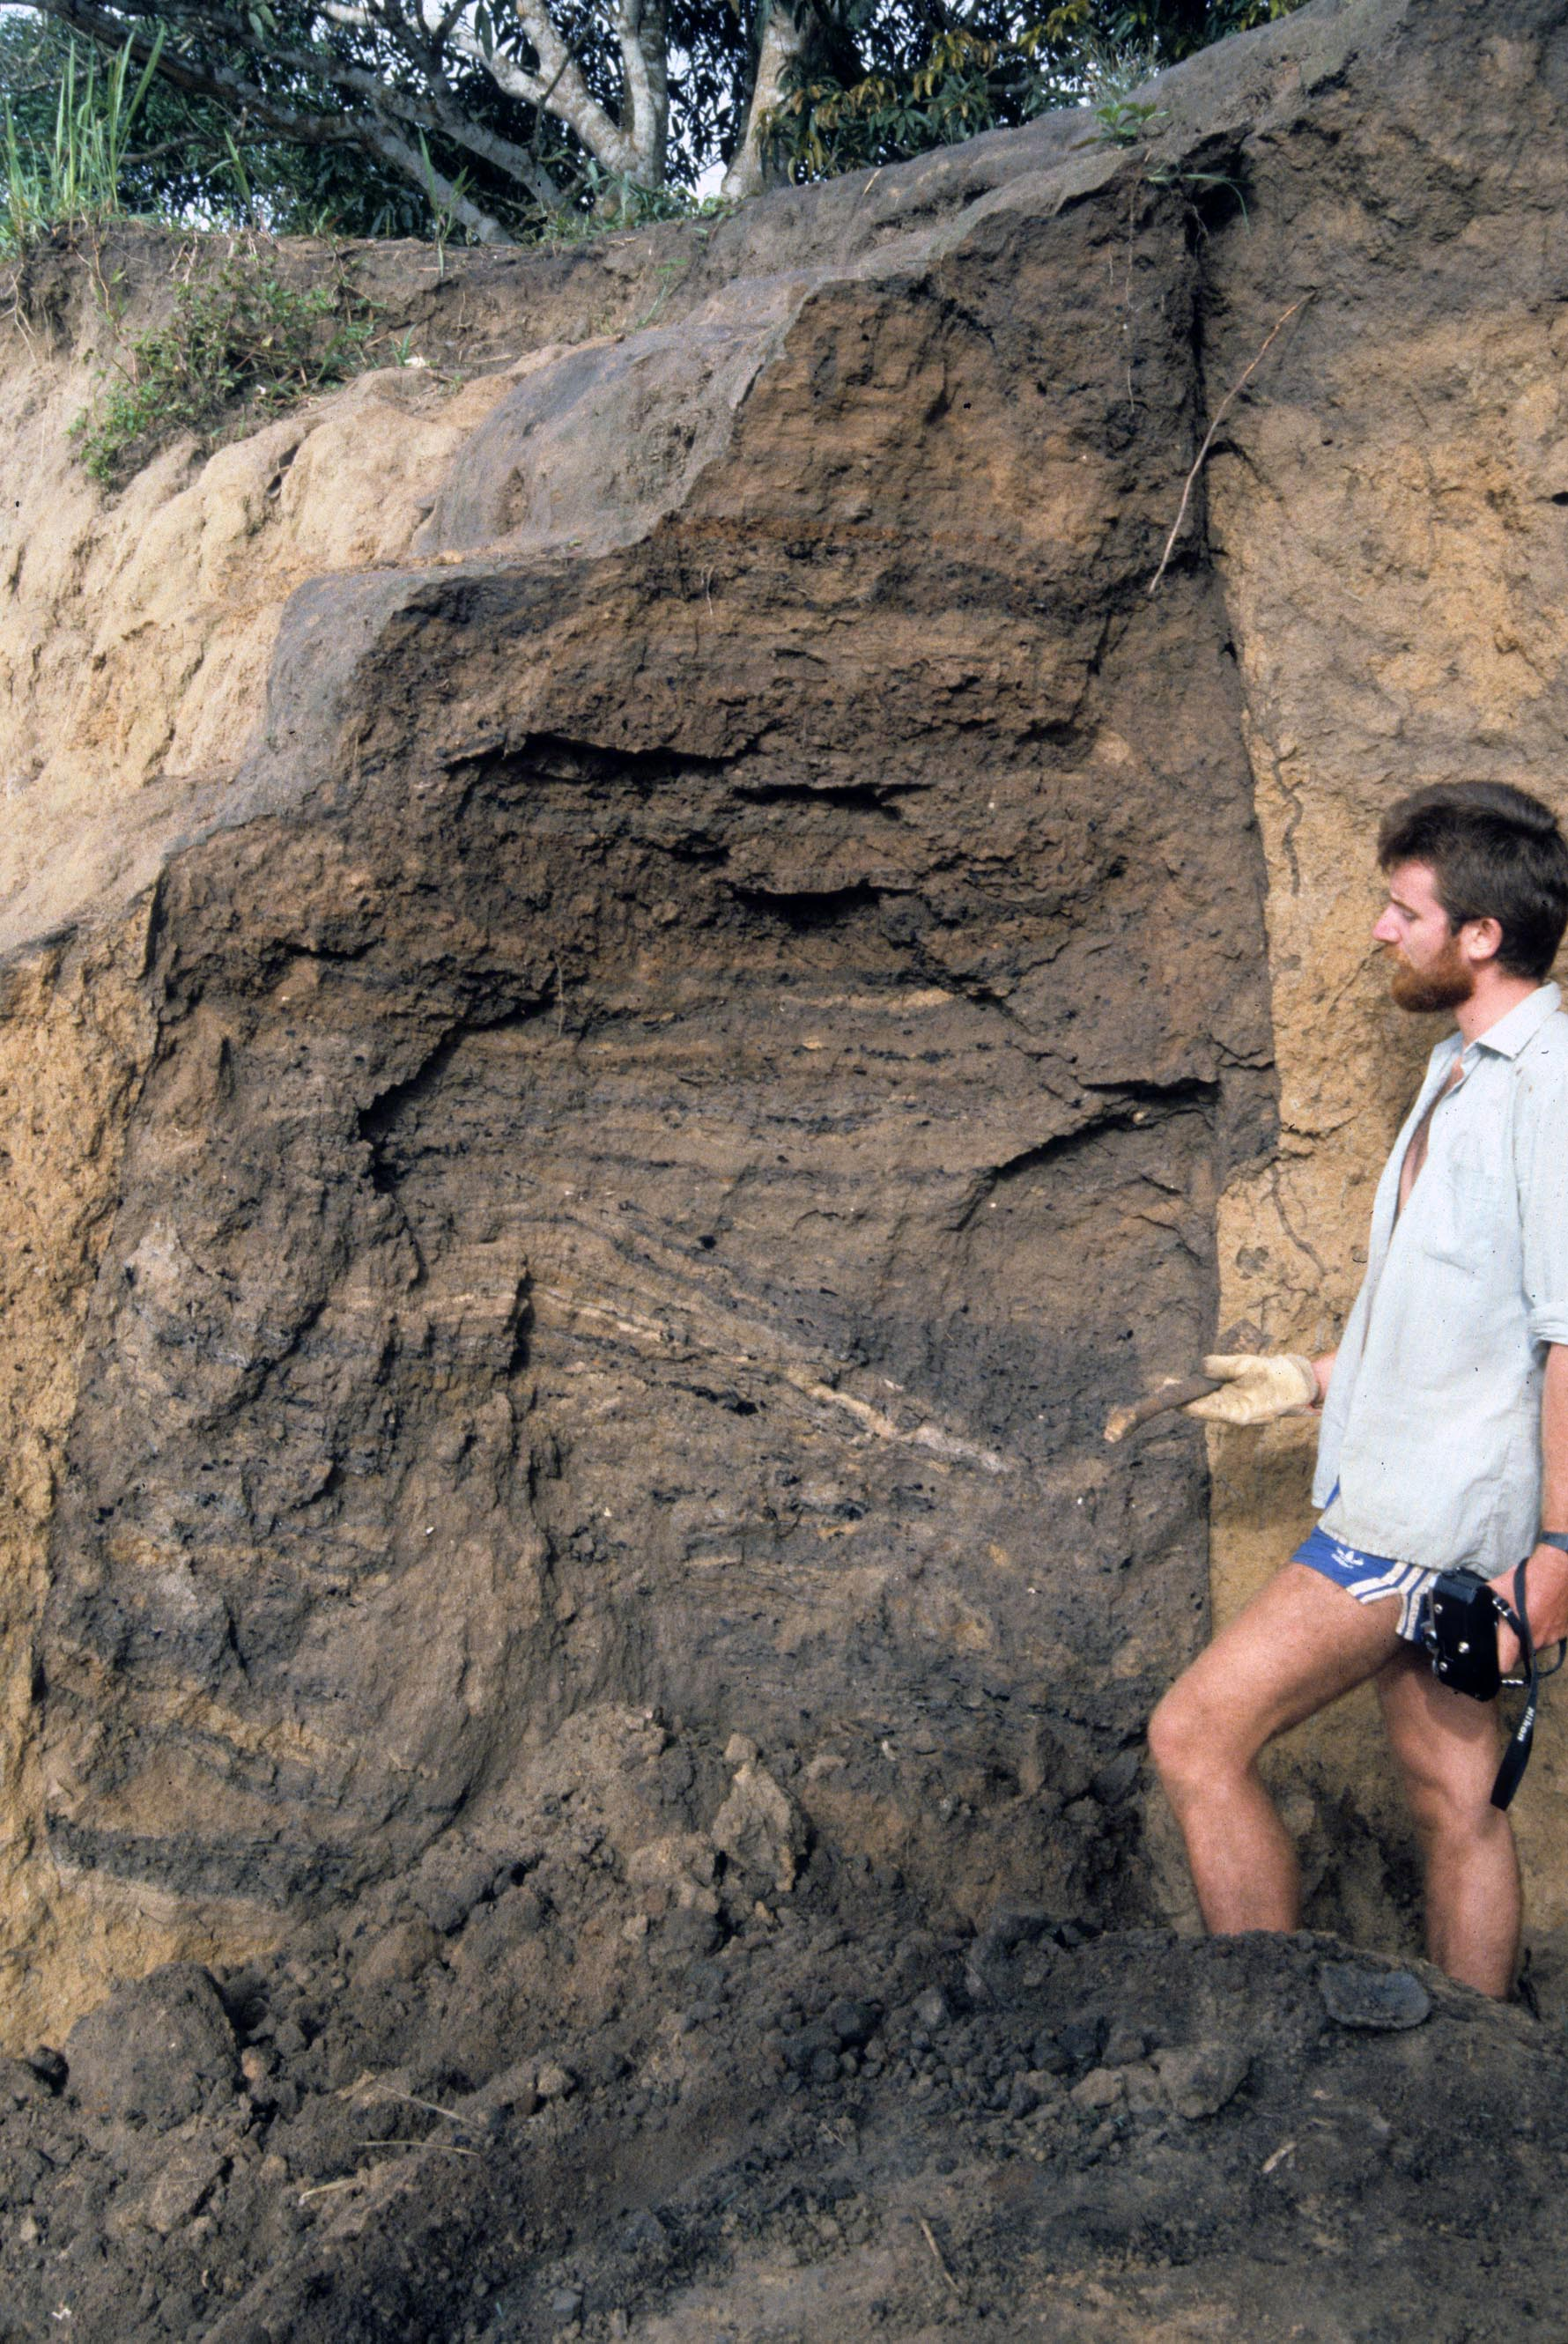
\includegraphics[width=\columnwidth]{fig/MLB85-103_E85-030-27.jpg}
		\captionof{figure}{MLB 85/103: Teilweise freierodierte Grube in der Uferböschung des Lua in Maluba (Foto: M. K. H. Eggert, 1985).\label{fig:MLB85-103_ProfilFoto}}
	\end{minipage}
\end{figure*}

\section*{\begin{tabular*}{\linewidth}{@{}l @{\extracolsep{\fill}} r@{}}
Nr.~4 & MLB~85/2\\
\end{tabular*} 
}

\textsf{\textbf{Maluba (Lua; Fpl.~230)}}

\vspace{1em}

\noindent\begin{tabular}{@{}rl@{}}
\textbf{Feldarbeit:} & \begin{tabular}[t]{@{}l@{}}\textbf{05.09.--06.09.1985 (C. Kanimba}\\ \textbf{Misago/H.-P. Wotzka)}\end{tabular} \\ 
\textbf{Abb.:} & \textbf{\ref{fig:MLB85-2_Prof_geputzt}} \\
\textbf{Lit.:} & \textbf{--} \\ 
\end{tabular}

\paragraph{Grabung und Befunde}\hspace{-.5em}|\hspace{.5em}%
Die 2,55\,m tiefe, kasten- bis leicht trapezförmige Grube zeichnete sich im Uferprofil durch eine scharf begrenzte dunkle Verfüllung ab. Sie hat einen Durchmesser von etwa 1,1~m, eine horizontale Sohle und vertikale bis leicht steilschräg überkippte Wandungen. Im unteren Teil weist sie eine horizontale, stark holzkohlehaltige, feine Bänderung auf. Direkt neben der Grube fand sich eine Körperbestattung, aus welcher kurz vor der Grabung bereits Skelettteile gefallen waren. Nach dem Profilputz ragten noch Knochen der unteren Extremitäten -- Unterschenkel und Fußwurzel sowie Teile der Mittelfußknochen, aber keine Zehen -- aus dem Profil (Abb.~\ref{fig:MLB85-2_Prof_geputzt}). Das Grab durchschneidet eine rot verziegelte \textit{Plattform} oder Feuerstelle. 

Im ersten Planum, das etwa 0,3\,m unter der rezenten Oberfläche lag, waren Grube und Bestattung deutlich voneinander unterscheidbar, ohne dass das zeitliche Verhältnis beider Befunde eindeutig war. Die von der Bestattung durchschnittene, gebänderte Lage angeziegelten Materials war über der Grube nicht erkennbar. Das Grab ist durchgehend etwa 0,4\,m breit. Seine dunkle Verfüllung ist stark mit hellen Sandflecken durchsetzt, während die Verfüllung der Grube homogen dunkelbraun ist und sich deutlich vom hellen anstehenden Sand absetzt.

Im Profil ist eine sehr fein laminierte Wechselschichtung von dunklen und hellen Lagen innerhalb der Grube erkennbar.\footnote{Die feine Wechselschichtung zusammen mit den scharfen Befundgrenzen kann als ein Indiz für ein junges Alter des Befundes gewertet werden. Die älteren, Keramik des Batalimo-Maluba-Stils enthaltenden und in die Jahrhunderte um die Zeitenwende datierten Gruben MLB~85/1-3-1 und MLB~85/1-3-2 (Kat.-Nr.~1--2) zeigen weder eine fein laminierte Schichtung noch scharfe Befundgrenzen.} Am zweiten Tag der Grabung stürzte aufgrund von starkem Regen das Profil teilweise ein. Die Grabung wurde danach nicht mehr weitergeführt.\footnote{Im eingestürzten Zustand konnte noch beobachtet werden, dass das Grab die Grube teilweise schneidet und somit stratigrafisch jünger ist. Die Bestattung ist bei dem Abrutschen des Materials  weiter herausgebrochen.}

\paragraph{Funde}\hspace{-.5em}|\hspace{.5em}%
Es lagen keine Funde aus dem Befund MLB~85/2 zur Auswertung vor.\footnote{Auf einigen der verfügbaren Situationsfotos, die währen der Anlage des ersten Abtrages gemacht wurden, ist zu sehen, dass Funde abgesammelt wurden und der Ausgräber C. Kanimba Misago neben sich ein Körbchen mit Scherben liegen hat. Was mit diesen Funden passiert ist und warum sie nicht beim restlichen Fundgut verblieben sind, lässt aus der vorhandenen Aktenlage nicht mehr rekonstruieren.} Da auch kein Probenmaterial für Radiokohlenstoffdatierungen vorliegt, ist eine Datierung des Befundes nicht möglich.

\section*{\begin{tabular*}{\linewidth}{@{}l @{\extracolsep{\fill}} r@{}}
Nr.~5 & MLB~85/103\\
\end{tabular*} 
}

\textsf{\textbf{Maluba (Lua; Fpl.~230)}}

\vspace{1em}

\noindent\begin{tabular}{@{}rl@{}}
\textbf{Feldarbeit:} & \textbf{05.09.1985 (M. K. H. Eggert)} \\ 
\textbf{Abb.:} & \textbf{\ref{fig:MLB85-103_ProfilFoto}} \\
\textbf{Taf.:} & \textbf{27.10--27.13} \\ 
\textbf{Lit.:} & \textbf{--} \\ 
\end{tabular}

\paragraph{Grabung und Befunde}\hspace{-.5em}|\hspace{.5em}%
Etwa 3\,m südwestlich der Grube MLB~85/2 (Kat.-Nr.~4) fand sich eine weitere, zwischen 2,7--3\,m tiefe Grube, mit einem Durchmesser von 1,5--1,6\,m (Abb.~\ref{fig:MLB85-103_ProfilFoto}).\footnote{Die Grube ist potenziell eher noch tiefer gewesen. Ein guter Teil des Befundes war bereits erodiert und zur rezenten Oberfläche des Dorfes fehlen einige Dezimeter.} Die vorhanden Fotos zeigen, dass die Grube eine horizontale Sohle sowie steilschräg überkippte Wandungen aufweist. Nach dem Einsturz des benachbarten Befundes MLB~85/2 wurde das Profil dieser Grube geputzt und einige Scherben abgesammelt.\footnote{Da keine Grabung erfolgte, wurde der Befund MLB~85/103 mit einer Kennung als Oberflächenkomplex aufgenommen.} Wie die Grube MLB~85/2 weist auch MLB~85/103 eine feine, lagige Verfüllung mit hellen, sandigen und dunklen, holzkohlehaltigen Schichten und eine scharfe Außengrenze auf (Abb.~\ref{fig:MLB85-103_ProfilFoto}).

\paragraph{Keramik\vspace{.5em}}\mbox{}\\
\begin{tabular}{@{}lrl@{}}
Bearbeitet:	& 829\,g & (100\,\%) \\ 
\end{tabular} 

\vspace{1em}
\noindent Das Inventar der aus dem Befund MLB~85/103 exemplarisch geborgenen Keramik umfasst unter anderem roulettverzierte Stücke. Insgesamt liegen aus dem Befund 15 GE vor, die nahezu alle am mittleren \mbox{Ubangi} angetroffenen Stilgruppen repräsentieren: eine GE des Batalimo-Maluba-Stils (Kap.~\ref{sec:BTM-Gr}), fünf GE der Dongo-Gruppe (Kap.~\ref{sec:DON-Gr}), eine GE der Bobulu-Gruppe (Kap.~\ref{sec:BBL-Gr}), zwei GE der Motenge-Boma-Gruppe (Kap.~\ref{sec:MTB-Gr}) sowie drei GE des rezenten Dama-Stils (Kap.~\ref{sec:DAM-Gr}). Daneben wurde noch eine mit Schnitzroulette verzierte Scherbe sowie zwei nicht genauer einzuordnende Stücke geborgen. Der Fund rezenter, mit \mbox{Roulette} verzierter Keramik unterstreicht das potenziell junge Alter des Befundes.



\begin{figure*}[!tb]
	\centering
	\begin{subfigure}[b]{.675\textwidth}
		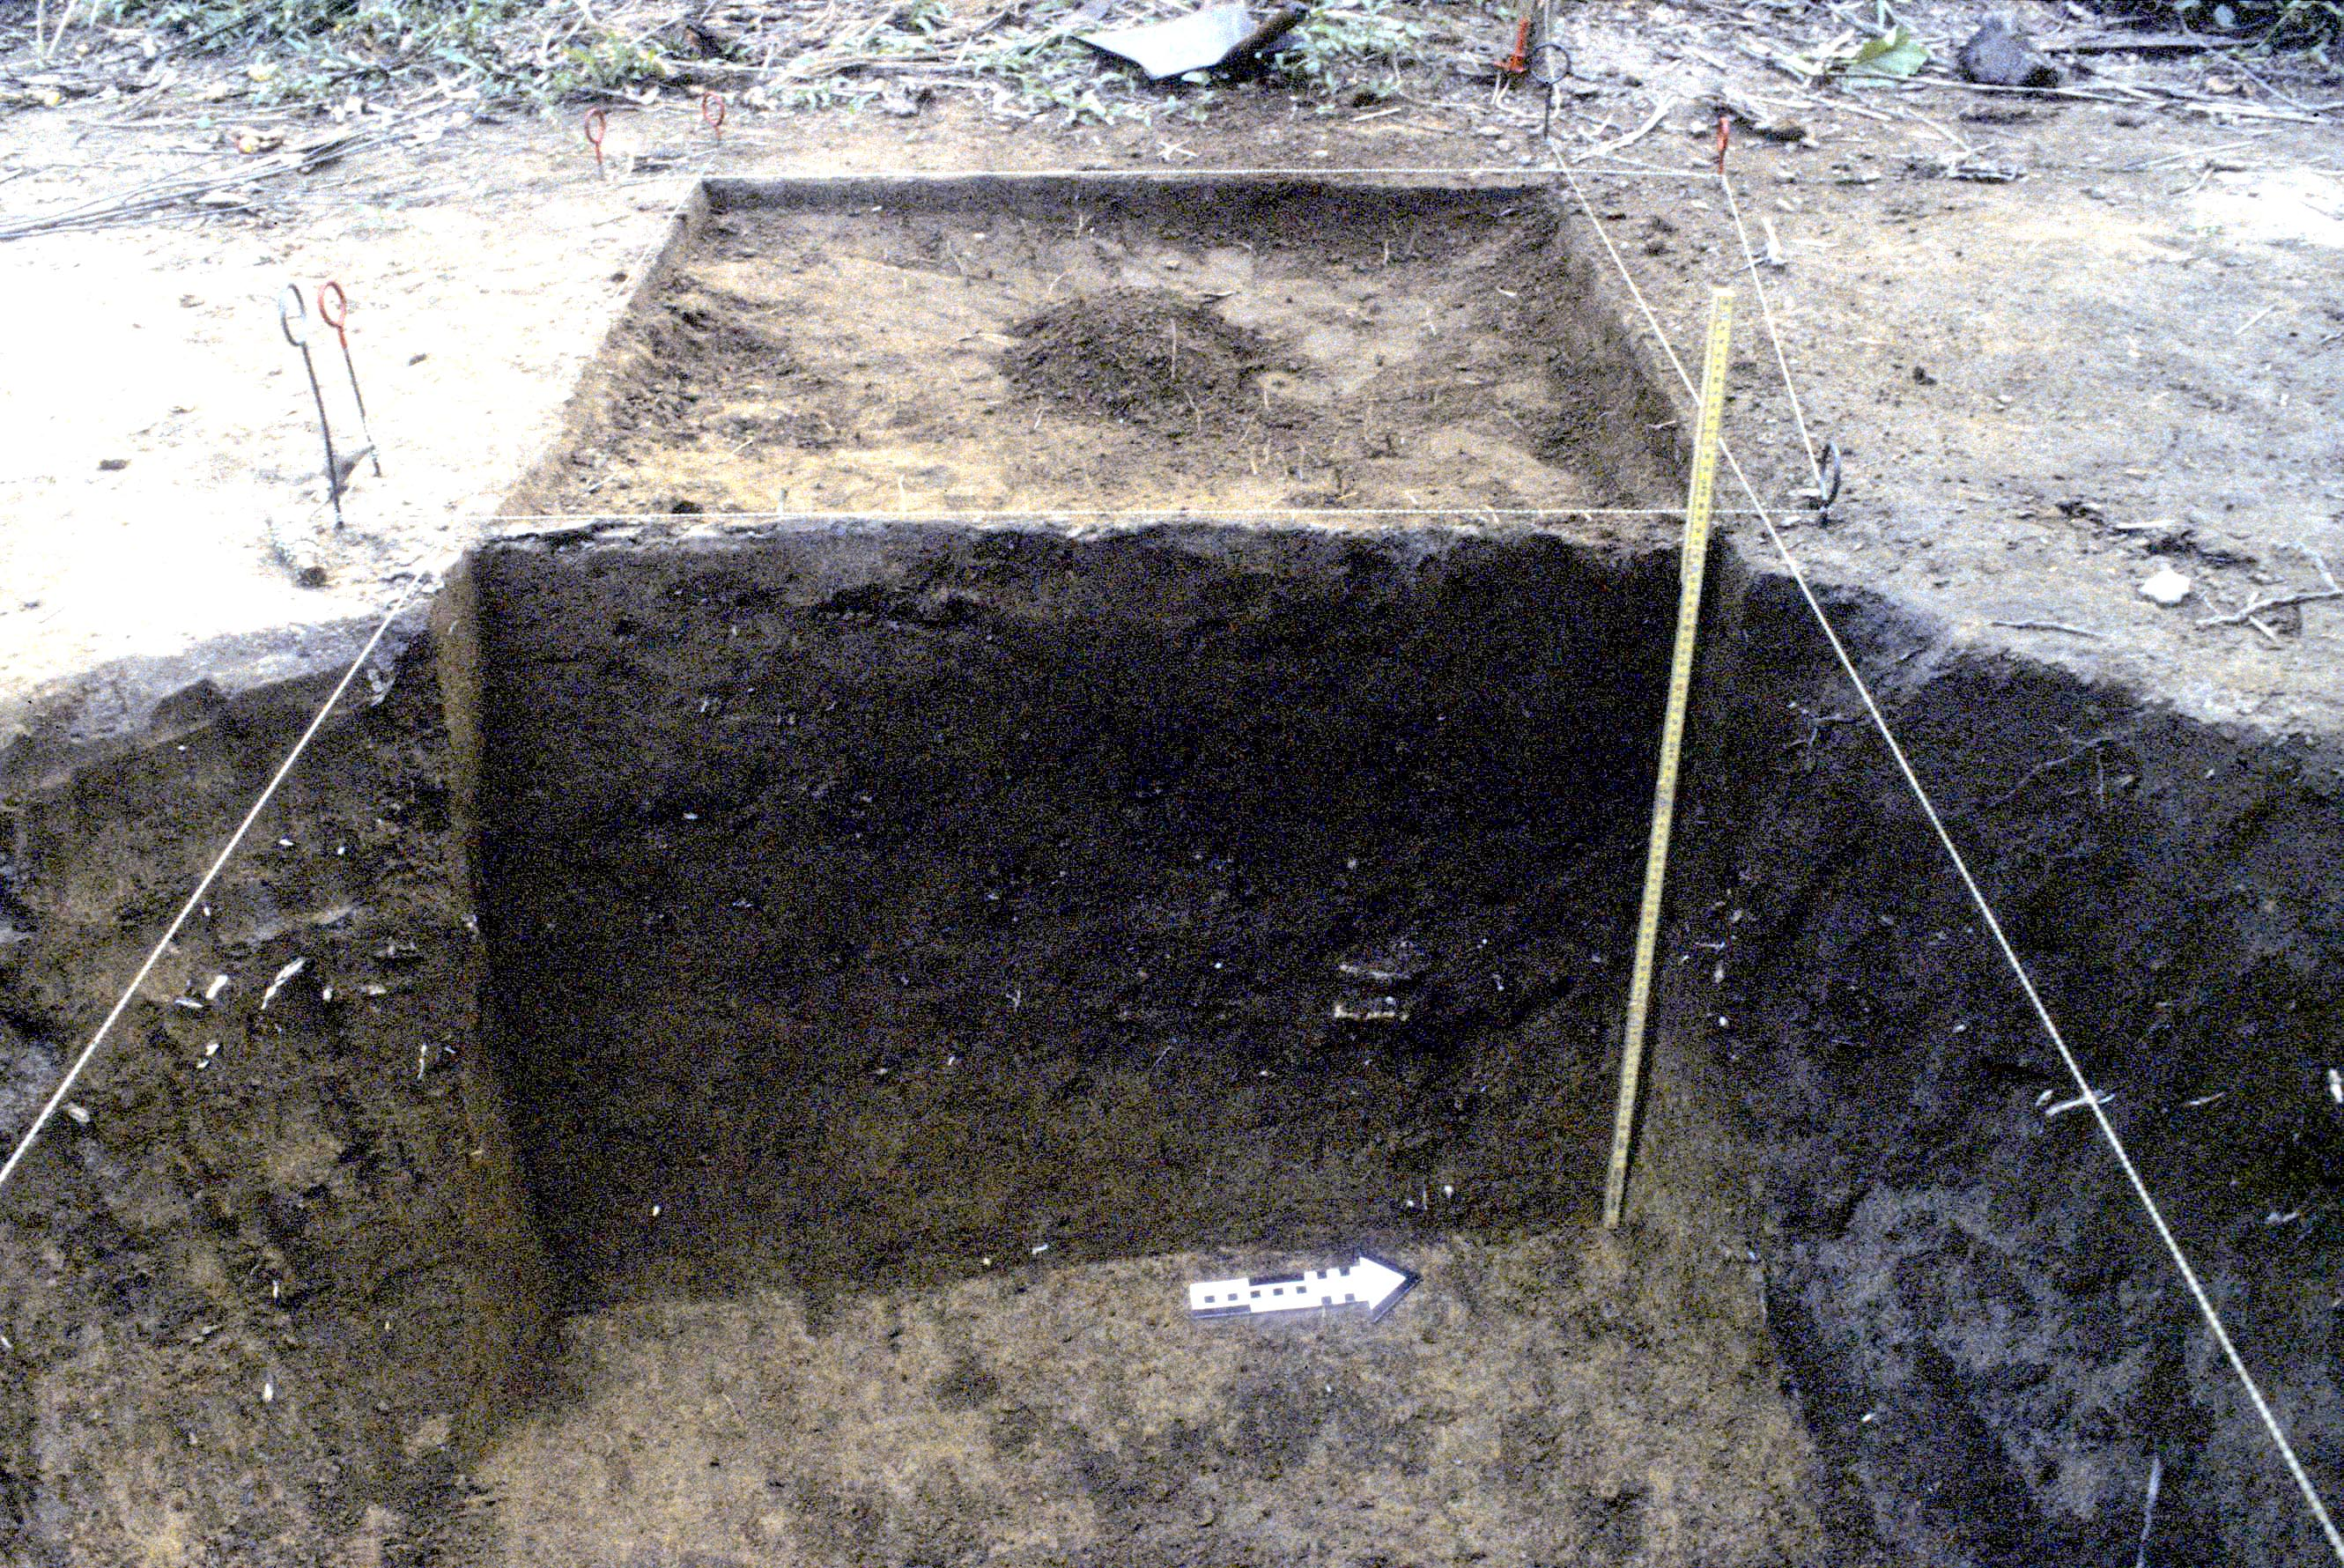
\includegraphics[width = \textwidth]{fig/BBS87-1_H87-01-4.jpg}
		\caption{Übersicht}
		\label{fig:BBS87-1_ProfilOst_Foto_Übersicht}
	\end{subfigure}\hfill
	\begin{subfigure}[b]{.30\textwidth}
		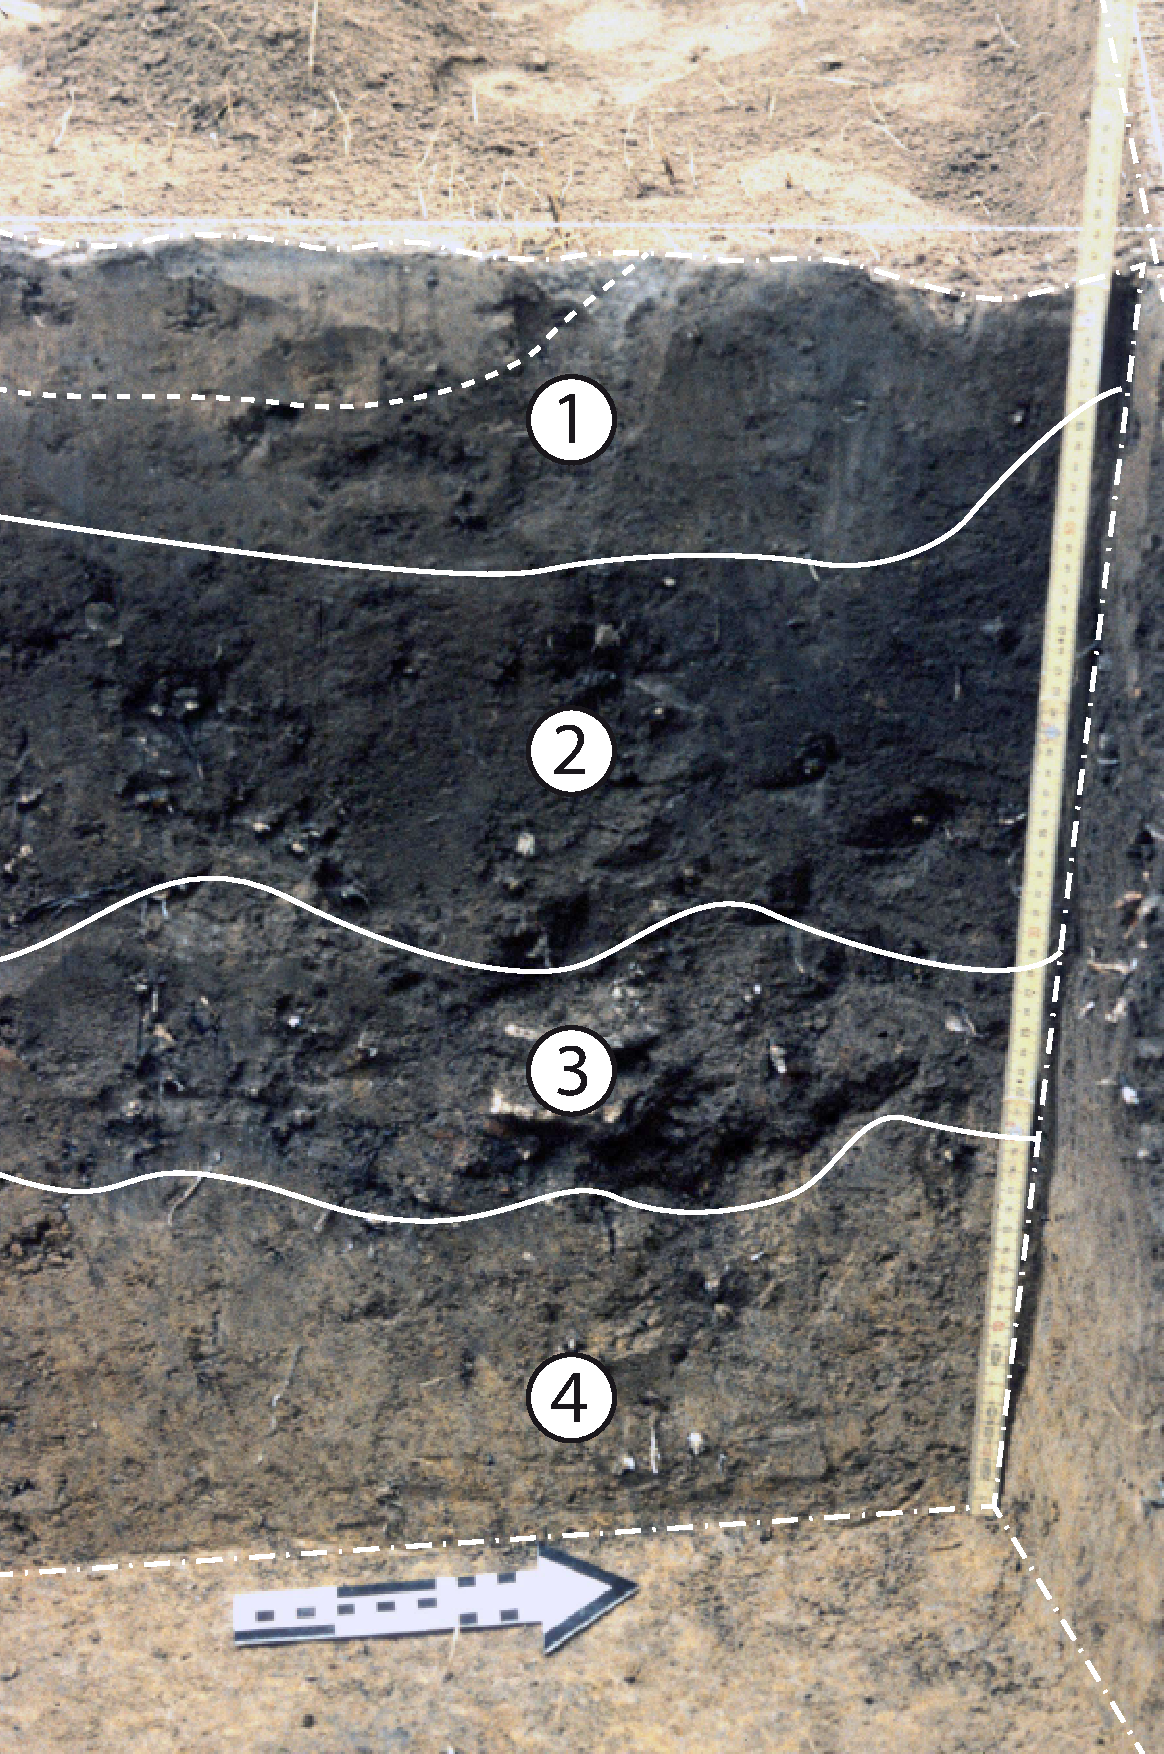
\includegraphics[width = \textwidth]{fig/BBS87-1_H87-01-2.pdf}
		\caption{Nördliche Hälfte}
		\label{fig:BBS87-1_ProfilOst_Foto_Detail}
	\end{subfigure}
	\caption{BBS 87/1: Kontrollprofil zu Beginn der Ausgrabung des 1$\times$1\,m großen Grabungsschnittes. Beide Aufnahmen stellen die einzige vorliegende Dokumentation der beobachteten Profile dar und waren im Original erheblich fehlbelichtet. Sie konnten lediglich bis zum hier abgebildeten Stand aufbereitet werden (Fotos: H. Holsten, 1987).}
	\label{fig:BBS87-1_ProfilOst_Foto}
\end{figure*}

\begin{table*}[tb]
	\centering
	{\footnotesize \begin{sftabular}{@{}lrrrr@{}}
\toprule
   \textbf{Fundkategorie} &  \textbf{Anzahl} &    \textbf{\%} &  \textbf{Gewicht (kg)} &    \textbf{\%} \\
\midrule
 gebrannter Lehm &       6 &   8,0 &          0,10 &  10,2 \\
         Keramik &      67 &  89,3 &          0,77 &  80,0 \\
        Schlacke &       1 &   1,3 &          0,05 &   5,1 \\
          Sonder &       1 &   1,3 &          0,04 &   4,7 \\
\bottomrule
\end{sftabular}
}
	\caption{BBS~87/1: Anteil verschiedener Fundmaterialien.}
	\label{tab:BBS87-1_Funde}
\end{table*}

\section*{\begin{tabular*}{\linewidth}{@{}l @{\extracolsep{\fill}} r@{}}
Nr.~6 & BBS~87/1\\
\end{tabular*} 
}

\textsf{\textbf{Bobusa (\mbox{Sangha}; Fpl.~239)}}

\vspace{1em}

\noindent\begin{tabular}{@{}rl@{}}
\textbf{Feldarbeit:} & \begin{tabular}[t]{@{}l@{}}\textbf{01.05.--03.05.1987}\\ \textbf{(C. Kanimba Misago)}\end{tabular} \\
\textbf{Abb.:} & \textbf{\ref{fig:BBS87-1_ProfilOst_Foto}--\ref{fig:BBS87_1_Funde}} \\
\textbf{Tab.:} & \textbf{\ref{tab:BBS87-1_Funde}}\\
\textbf{Taf.:} & \textbf{33.12--33.15} \\ 
\textbf{Lit.:} & \textbf{--} \\ 
\end{tabular}

\paragraph{Grabung und Befunde}\hspace{-.5em}|\hspace{.5em}%
Das Dorf Bobusa liegt etwa 20\,km nördlich der Mündung des \mbox{Sangha} in den Kongo und bei umfangreichen Prospektionen wurden zwei offene Lehmentnahmegruben entdeckt, in denen sich Keramik fand. Ausgehend von den beiden Gruben wurde jeweils ein 1\,$\times$\,1\,m großer Testschnitt angelegt, der die in den Gruben sichtbare Schicht-Abfolge erfassen sollte. Für den Schnittkasten BBS~87/2 (Kat.-Nr.~7) liegt die Dokumentation des Ausgräbers Hermann Holsten vor, während die Unterlagen zum durch C. Kanimba Misago ausgegrabenen Testschnitt BBS~87/1 verschollen sind. Aus den vorliegenden Fotos, die sämtlich von H. Holsten als Situationsfotos angefertigt wurden, und den Tagebuchnotizen von M.~K.~H. Eggert lässt sich das Folgende rekonstruieren: Im westlichen Teil einer etwa 2--2,5\,m großen und 0,6--0,7\,m tiefen Lehmentnahmegrube wurde ein Profil angelegt, welches zugleich das Ost-Profil des davon ausgehenden Grabungsschnittes BBS~87/1 bildete.\footnote{Das einzige Foto des Ostprofils zeigt dieses nicht in seiner Gänze, sondern lediglich die nördliche Hälfte (Abb.~\ref{fig:BBS87-1_ProfilOst_Foto_Detail}). Das Bild diente wohl der Dokumentation zweier, im Profil steckenden großer -- nicht mehr genau identifizierbarer -- Keramikscherben oder Knochenstücke in Schicht~3, etwa 0,35--0,4\,m unter der Oberfläche.} Im Anschluss an die Dokumentation dieses Profils wurde eine 1\,$\times$\,1\,m große Fläche in drei Abträgen ausgegraben.

Auf Basis aller vorliegenden Informationen können einige Angaben zur stratigrafischen Situation gemacht werden. Das Fundinventar ist mit Abtragsnummern zwischen 1--3 beschriftet worden und auch im benachbarten Befund BBS~87/2 (Kat.-Nr.~7) wurde so verfahren, dass ein Abtrag grob einer im Profil beobachteten Schicht entsprach. Bei der Betrachtung des verfügbaren Detailfotos des Ost-Profils (Abb.~\ref{fig:BBS87-1_ProfilOst_Foto_Detail}) lassen sich drei Fund-Schichten unterscheiden. Eine dunkelgraue bis schwarze Schicht~2 liegt zwischen den helleren, grauen Schichten~1 und 3. Dieses Schicht-Paket sitzt wiederum auf dem anstehenden Lehm auf (Abb.~\ref{fig:BBS87-1_ProfilOst_Foto}: 4). Es kann daher als Hypothese gelten, dass die Funde der drei Abträge die Schichten im Ost-Profil nachzeichnen.

\begin{figure*}[p]
	\centering
	\begin{subfigure}[t]{\textwidth}
		\centering
		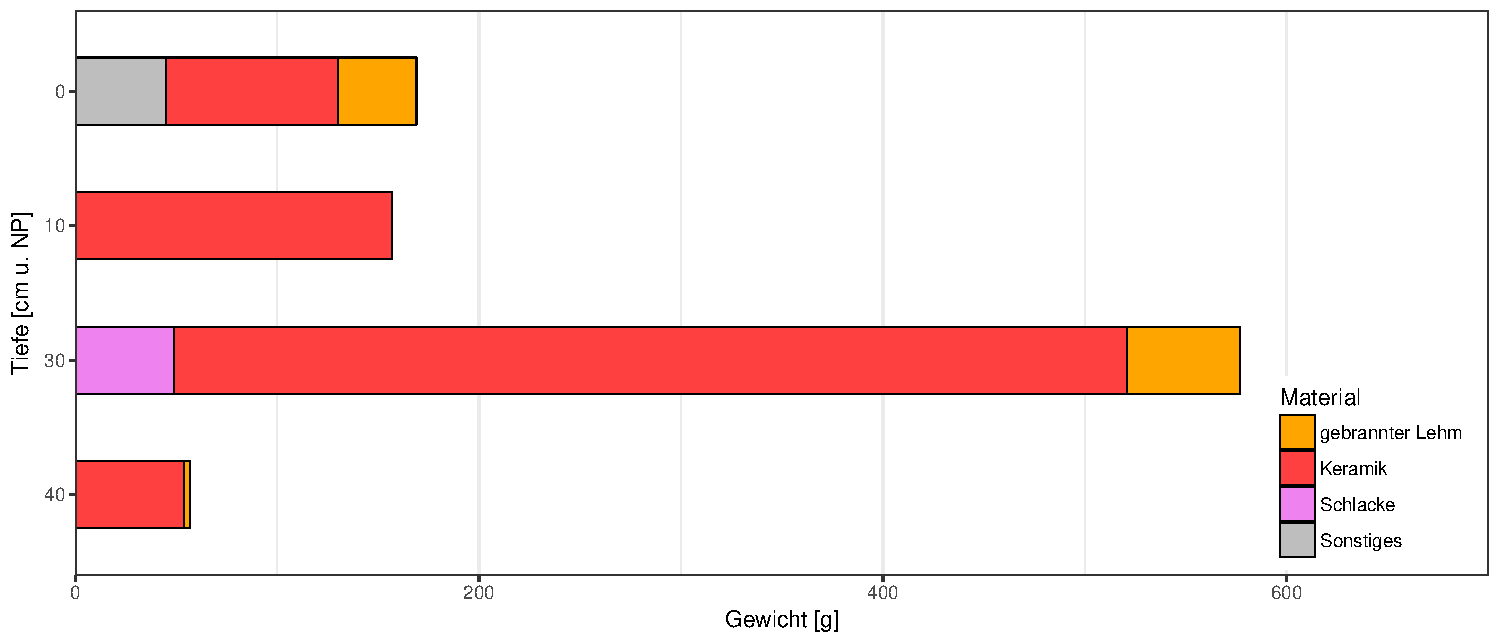
\includegraphics[width=\textwidth]{fig/9-6_BBS87-1_VerteilungFunde_R.pdf}
		\caption{Fundmaterial.\vspace{1em}}
		\label{fig:BBS87-1_VerteilungFunde}
	\end{subfigure}
	\begin{subfigure}[t]{\textwidth}
		\centering
		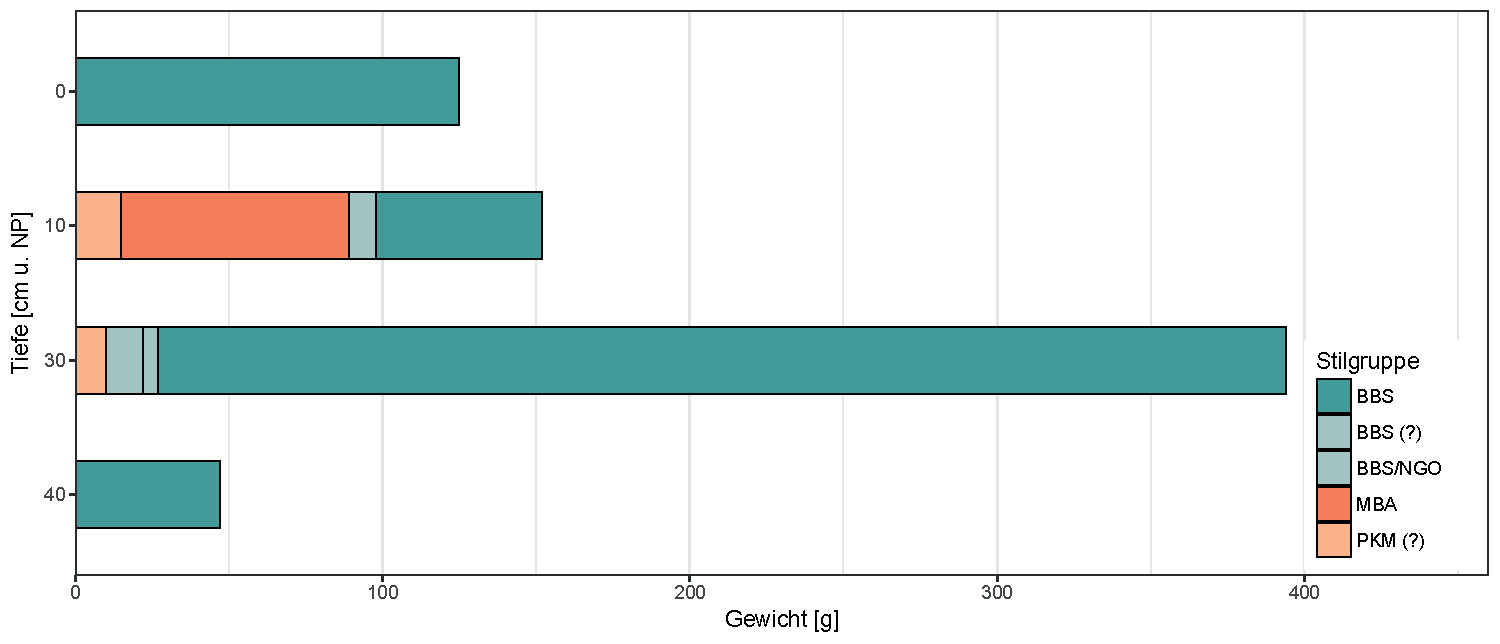
\includegraphics[width=\textwidth]{fig/9-6_BBS87-1_KeramikStilgruppen_R.pdf}
		\caption{Keramische Stilgruppen.\vspace{1em}}
		\label{fig:BBS87-1_VerteilungStilgr}
	\end{subfigure}
	\begin{subfigure}[t]{\textwidth}
		\centering
		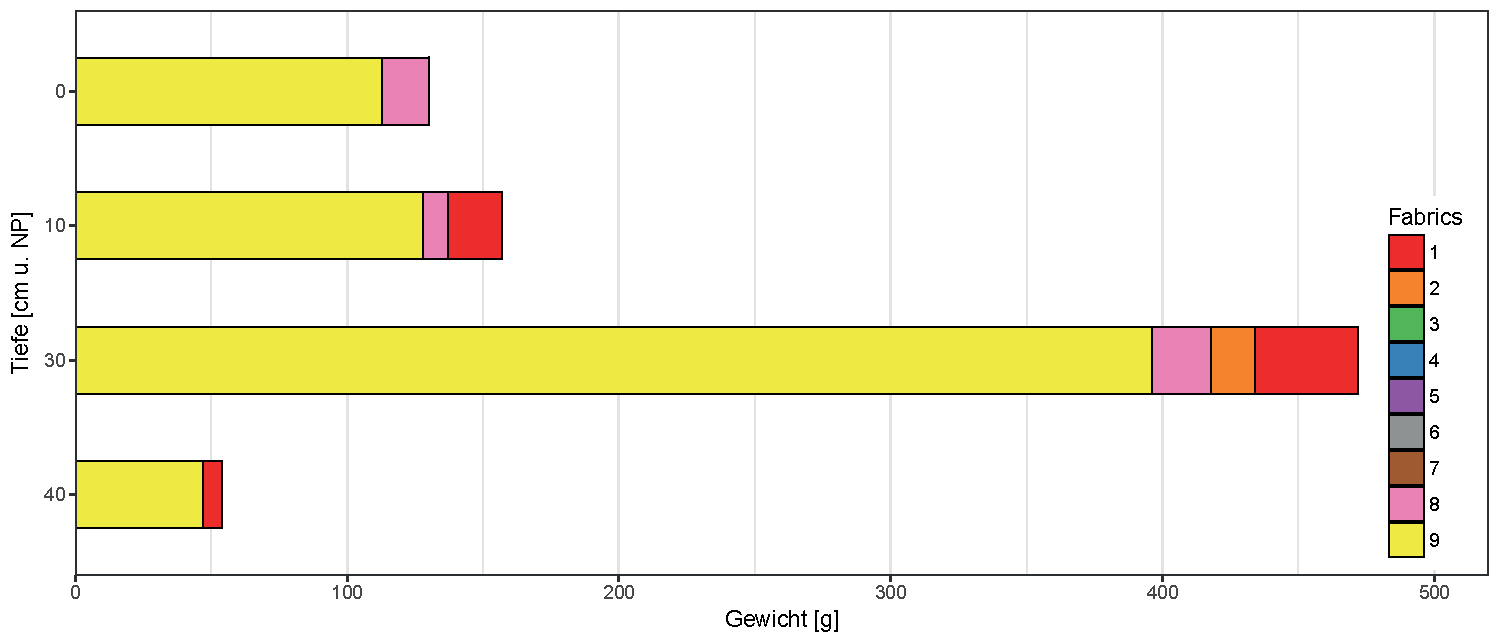
\includegraphics[width=\textwidth]{fig/9-6_BBS87-1_Fabrics_R.pdf}
		\caption{\textit{Fabrics}.}
		\label{fig:BBS87-1_VerteilungFabrics}
	\end{subfigure}
	\caption{BBS 87/1: Verteilung der Fundmaterialien (A), keramischen Stilgruppen (B) und \textit{Fabrics} (C) in den entsprechenden Tiefen der Grabung.}
	\label{fig:BBS87_1_Funde}
\end{figure*}

\begin{figure*}[tb]
	\centering
	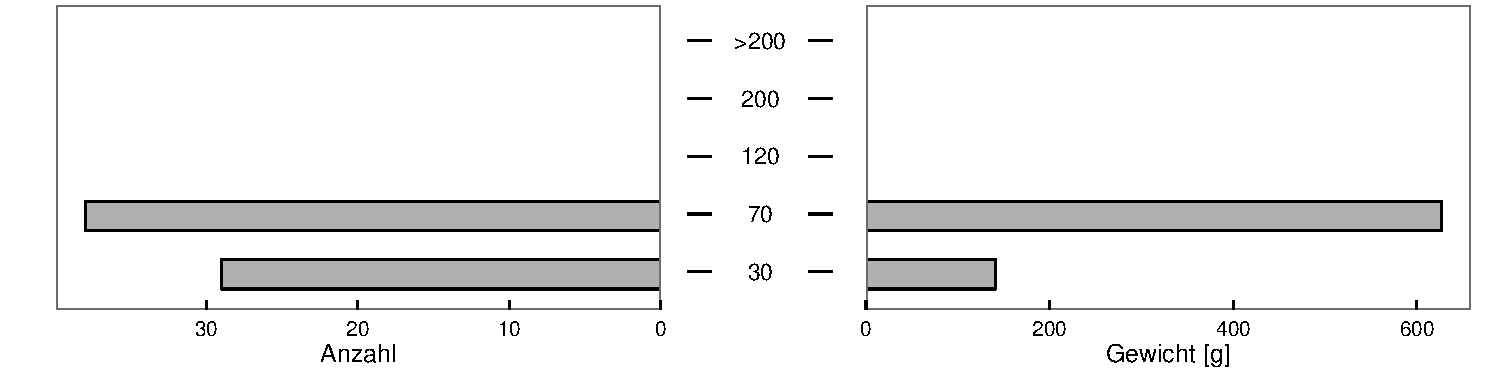
\includegraphics[width=\textwidth]{fig/9-6_BBS87-1_Fragmentierung_2.pdf}
	\caption{BBS~87/1: Fragmentierungsgrad der Scherben (n~=~67; Größenklassen siehe Anm.~\ref{ftn:Keramik_Fragmentierung}).}
	\label{fig:Fragmenierung_BBS87-1}
\end{figure*}

\vspace{.5em}\noindent Die Grabung erbrachte -- vor dem Hintergrund der geschilderten Rekonstruktion -- den folgenden stratigrafischen Befund (Abb.~\ref{fig:BBS87-1_ProfilOst_Foto}):\footnote{Tiefenangaben beziehen sich auf die rezente Oberfläche und wurden von den Fotos abgenommen (Abb.~\ref{fig:BBS87-1_ProfilOst_Foto}).}
\begin{itemize}[leftmargin=*, labelindent=1em, noitemsep, topsep=0pt]
\item [(1)] 0--0,1\,m; dunkel/leicht grau; heller als (2)
\item [(2)] 0,1--0,3\,m; sehr dunkel/schwarz
\item [(3)] 0,3--0,4\,m; heller als (2); potenziell kompakter beziehungsweise fester als (1) und (2)
\item [(4)] \textgreater\,0,4\,m; anstehender Lehm
\end{itemize}

\paragraph{Keramik\vspace{.5em}}\mbox{}\\
\begin{tabular}{@{}lrl@{}}
Ausgezählt: & 317\,g & \\ 
Bearbeitet: & 451\,g & (59\,\%) \\ 
Insgesamt: & 768\,g & \\ 
\end{tabular} 

\vspace{1em}\noindent Die Grabung BBS~87/101 erbrachte zusammengenommen nur etwas unter 1\,kg Fundmaterial, 80\,\% davon Keramik (Tab.~\ref{tab:BBS87-1_Funde}). Der Großteil stammt aus dem zweiten Abtrag, zwischen 0,1--0,3\,m unter der Oberfläche (Abb.~\ref{fig:BBS87-1_VerteilungFunde}). Es fanden sich keine Stücke, die größer als 70\,$\times$\,70\,mm waren (Abb.~\ref{fig:Fragmenierung_BBS87-1}). Aufgrund des hohen Zerscherbtheitsgrades war eine Stilgruppenansprache nur selten möglich. 

Der Großteil des keramischen Inventars sind formal kaum diagnostische Merkmale aufweisende Scherben mit Schamott-Magerung (87\,\%), die der Bobusa-Gruppe zugerechnet werden (Kap.~\ref{sec:BBS-Gr}). Im ersten, Schicht~1 repräsentierenden Abtrag fand sich das Fragment eines stark bauchigen Gefäßes mit gekehlter Schulter, das dem Mbandaka-Stil des Inneren Konogbeckens \parencite[139--143; Kap.~\ref{sec:MBA-Gr}]{Wotzka.1995} zugerechnet werden kann. Fragmente einer kleinen, rundbauchigen Flasche mit gekehlter Schulter und langem Kegelhals sind ebenfalls der Mbandaka-Gruppe zuzurechnen (Taf.~33.15). Beide Stücke weisen eine auffällige Schamott-Magerung auf. In technischer Sicht unterschieden sie sich nicht vom sonstigen Material aus Bobusa. Im Material des ersten Abtrages befinden sich auch zwei Scherben, die stilistisch wie technisch an die Pikunda-Munda-Gruppe (Kap.~\ref{sec:PKM-Gr}) erinnern.\footnote{Beide Stücke weisen neben horizontalen Rillen auch Wiegebandverzierung auf. Letztere konnte auf Schamott-gemagerter Keramik bislang nicht beobachtet werden. Eines der Stücke ist ein leicht konvexer, ausbiegender Rand, während das zweite Stück das Fragment eines Gefäßes mit gerader oder leicht konvexer Schulter ist.} GE ohne Schamott-Magerung sind kaum vertreten. Eine stratigrafische Abfolge der keramischen Stilgruppen innerhalb der Schichten, welche im Sinne einer chronologischen Gliederung interpretiert werden könnte, kann aus dem vorliegenden Material nicht abgeleitet werden.

\paragraph{Sonstige Funde}\hspace{-.5em}|\hspace{.5em}%
An der Oberfläche fand sich ein keramischer Flaschenstöpsel (Taf.~33.13) und im zweiten, die Schicht~2 repräsentierenden Abtrag ein kantiges Stücke metallisch graulicher, kompakter Schlacke (Abb.~\ref{fig:BBS87-1_VerteilungFunde}).

\paragraph{Datierung}\hspace{-.5em}|\hspace{.5em}%
Das Fundinventar des Schnitts BBS~87/1 setzt sich größtenteils aus dem gegenwärtig nicht direkt zu datierenden Bobusa-Stil zusammen (Kap.~\ref{sec:BBS-Gr}). Lediglich aufgrund loser morphologischer, ornamentaler sowie technischer Ähnlichkeiten lässt es sich in Relation zur Keramik von der gegenwärtig nicht hinreichend ausgewerteten Fundstelle Île des Mimosas im Stadtgebiet von Kinshasa setzen \parencite[siehe][279\,f.]{Eggert.1984}. Die dortigen Funde sind auf Basis einer Radiokohlenstoffdatierung in das 2. bis 4.~Jh. n.~Chr. datiert. Daneben finden sich Vertreter des Pikunda-Munda-Stils (Kap.~\ref{sec:PKM-Gr}) sowie der in die Jüngere Eisenzeit datierenden Stile Mbdandaka (Kap.~\ref{sec:MBA-Gr}) und -- unter Vorbehalt -- Ngombe (Kap.~\ref{sec:NGO-Gr}; Abb.~\ref{fig:BBS87-1_VerteilungStilgr}). 

\paragraph{Interpretation}\hspace{-.5em}|\hspace{.5em}%
Aufgrund des Fehlens der Dokumentation lassen sich nur auf indirektem Wege Rückschlüsse auf die angetroffene Befundsituation ziehen. Eine Deutung der beobachteten Schichten ist auf dieser Basis nicht möglich.

\begin{figure*}[!tb]
	\centering
	\begin{subfigure}[b]{\columnwidth}
		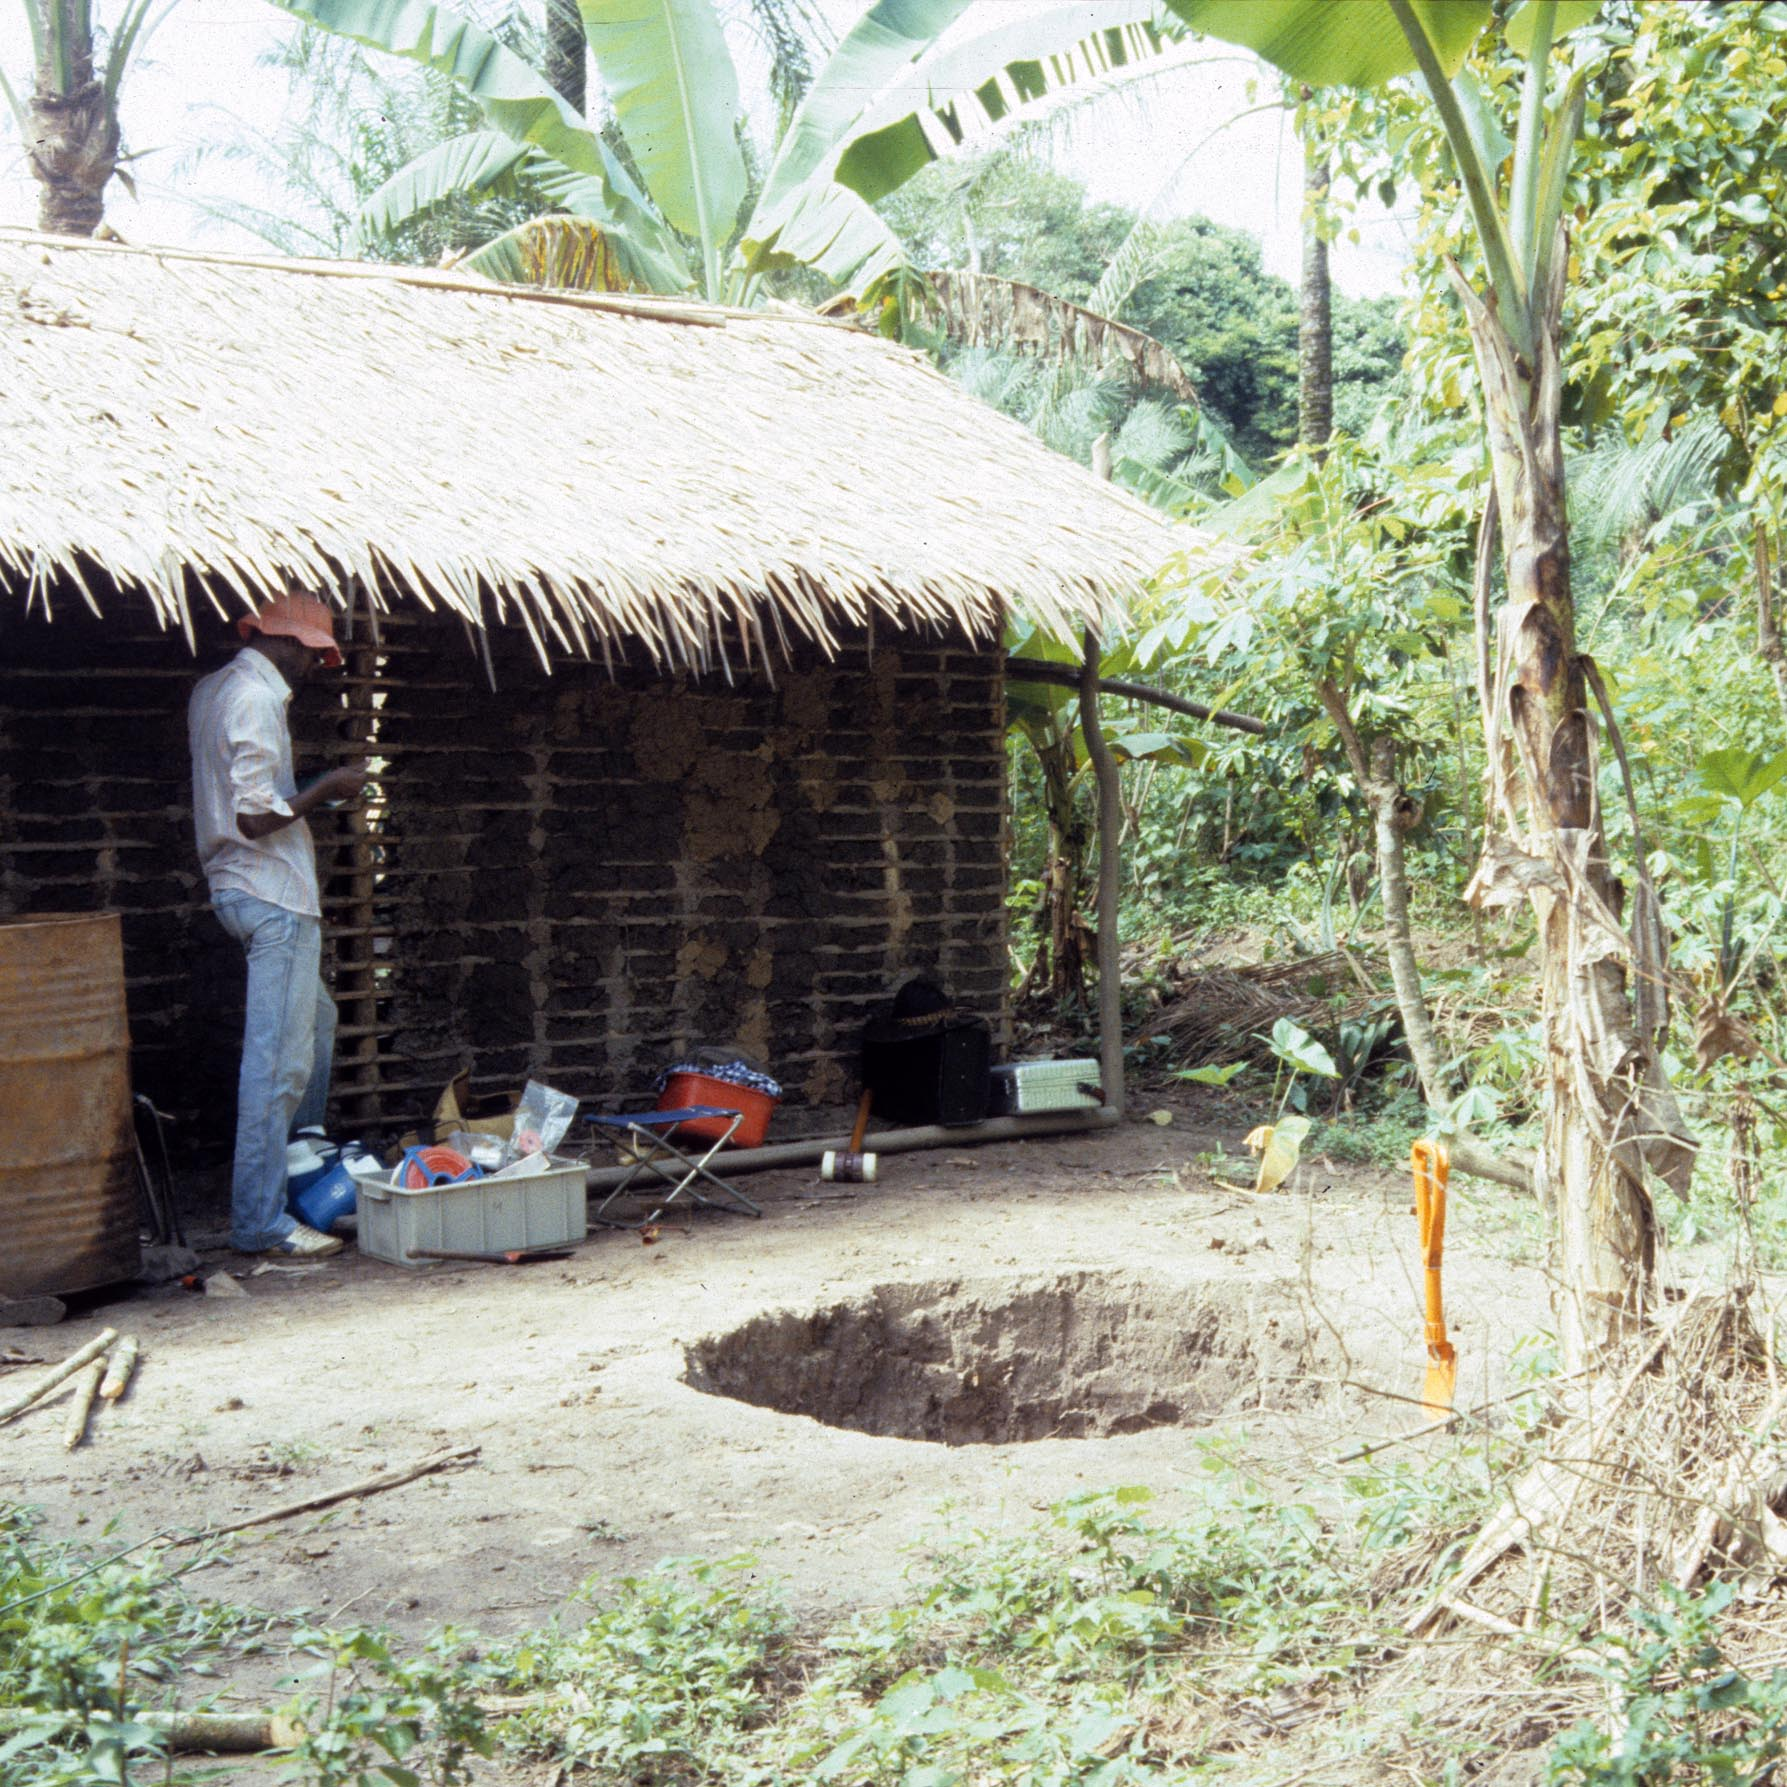
\includegraphics[width = \textwidth]{fig/BBS87-2_E87-02-17.jpg}
		\caption{Überblick über die Grabungsstelle (Foto: M. K. H. Eggert, 1987)}
		\label{fig:BBS87-2_GrubeVorGrabung}
	\end{subfigure}\hfill
	\begin{subfigure}[b]{\columnwidth}
		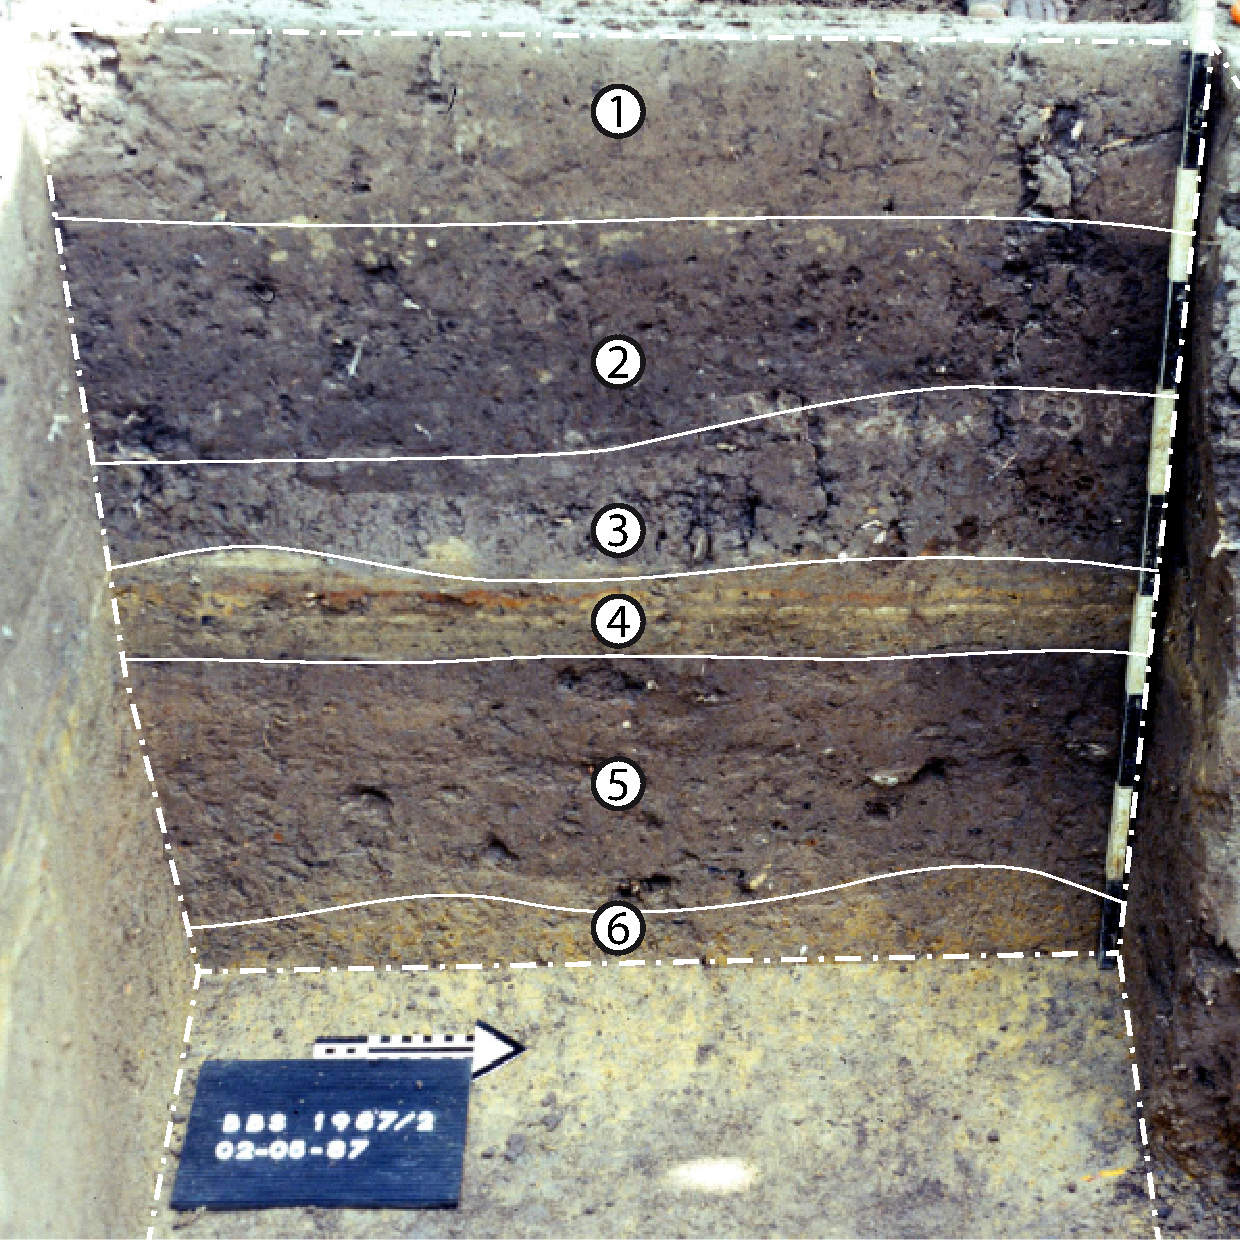
\includegraphics[width = \textwidth]{fig/BBS87-2_H87-01-5.pdf}
		\caption{Kontrollprofil (Foto: H. Holsten, 1987)}
		\label{fig:BBS87-2_OstProfil}
	\end{subfigure}
	\caption{BBS 87/2: Grabungsstelle vor der Untersuchung von Nordwesten (\textbf{A}) und das Kontrollprofil (Ostprofil des Schnitts) vor der Grabung (\textbf{B}).}
	\label{fig:BBS87-2_GrubeVorGrabung_OstProfil}
\end{figure*}

\section*{\begin{tabular*}{\linewidth}{@{}l @{\extracolsep{\fill}} r@{}}
Nr.~7 & BBS~87/2\\
\end{tabular*} 
}

\textsf{\textbf{Bobusa (\mbox{Sangha}; Fpl.~239)}}

\vspace{1em}

\noindent\begin{tabular}{@{}rl@{}}
\textbf{Feldarbeit:} & \textbf{01.05.--05.05.1987 (H. Holsten)} \\ 
\textbf{Abb.:} & \textbf{\ref{fig:BBS87-2_GrubeVorGrabung_OstProfil}--\ref{fig:BBS87-2_Eisenspitze}} \\
\textbf{Tab.:} & \textbf{\ref{tab:BBS87-2_Funde}}\\
\textbf{Taf.:} & \textbf{33.16--33.17} \\ 
\textbf{Lit.:} & \textbf{--} \\ 
\end{tabular}

\paragraph{Grabung und Befunde}\hspace{-.5em}|\hspace{.5em}%
Die Grabung BBS~87/2 erfasste die Befundsituation ausgehend von einer etwa 0,9--1,6\,m großen und knapp 1\,m tiefen Lehmentnahmegrube. Im Anschluss an die Dokumentation des im westlichen Teil der Grube angelegten Profils wurden die fünf sichtbaren Schichten (Abb.~\ref{fig:BBS87-2_GrubeVorGrabung_OstProfil}) in einem 1\,$\times$\,1\,m großen Schnitt ausgegraben.\footnote{Die Abträge zeichnen dabei die im Ost-Profil beobachteten Schichten grob nach, ohne dass explizit nach natürlichen Schichten gegraben wurde.} 

Die Grabung erbrachte drei nahezu fundfreie, dunkel- bis mittelbraune Schichten (1--3), die untereinander nur schwach abgegrenzt waren (Abb.~\ref{fig:BBS87-2_GrubeVorGrabung_OstProfil}). Darauf folgt ein auffällig scharf nach oben abgegrenztes, fein laminiertes, hellgelbes lehmiges \textit{Paket}~4. Schicht~2 überlagert sowohl das lehmige \textit{Paket}~4, als auch die Verfüllung (Schicht~3) einer wannenartigen, 0,1--0,15 m tiefen Eingrabung in das Schicht-Paket~4 (Abb.~\ref{fig:BBS87-2_T76Skizze}--C). Das Schicht-Paket~4 ist mit feinen dunklen, Holzkohle-haltigen sowie roten, angeziegelten Linsen durchzogen. Ein innerhalb des Schicht-Paketes~4 bei etwa 0,6\,m unter der rezenten Oberfläche angelegtes Planum\footnote{Während die Profile gezeichnet und fotografiert wurden (Abb.~\ref{fig:BBS87-2_Profile}), liegen von den angelegten Plana nur einige Fotos und Skizzen vor (Abb.~\ref{fig:BBS87-2_Plana_Foto+Skizzen}).} war stark mit Holzkohle durchsetzt (Abb.~\ref{fig:BBS87-2_T83Skizze}--E). Im östlichen Teil dieses Planums zeigte sich ein sehr flacher, stark rötlich verfärbter Bereich, der als Feuerstelle interpretiert werden kann. 

\begin{figure*}[p]
	\centering
	\begin{subfigure}[t]{.75\textwidth}
		\includegraphics[width = \textwidth, page = 1]{fig/BBS87-2_Plana.pdf}
		\caption{Übersicht über die Profile}
		\label{fig:BBS87-2_SkizzeUebersicht}
	\end{subfigure}
	\begin{subfigure}[t]{.75\columnwidth}
		\includegraphics[width = \columnwidth, page = 2]{fig/BBS87-2_Plana.pdf}
		\caption{Planumsskizze bei zirka 0,5\,m unter Oberfläche (T76)}
		\label{fig:BBS87-2_T76Skizze}
	\end{subfigure}\hspace{1em}
	\begin{subfigure}[t]{.75\columnwidth}
		\includegraphics[width = \columnwidth, page = 3]{fig/BBS87-2_Plana.pdf}
		\caption{Planumsfoto bei zirka 0,5\,m unter Oberfläche (T76; Foto: H. Holsten, 1987)}
		\label{fig:BBS87-2_T76Foto}
		\end{subfigure}
	\begin{subfigure}[t]{.75\columnwidth}
		\includegraphics[width = \columnwidth, page = 4]{fig/BBS87-2_Plana.pdf}
		\caption{Planumsskizze bei zirka 0,6\,m unter Oberfläche (T83)}
		\label{fig:BBS87-2_T83Skizze}
		\end{subfigure}\hspace{1em}
	\begin{subfigure}[t]{.75\columnwidth}
		\includegraphics[width = \columnwidth, page = 5]{fig/BBS87-2_Plana.pdf}
		\caption{Planumsfoto bei zirka 0,6\,m unter Oberfläche (T83; Foto: H. Holsten, 1987)}
		\label{fig:BBS87-2_T83Foto}
		\end{subfigure}
	\begin{subfigure}[t]{.75\columnwidth}
		\includegraphics[width = \columnwidth, page = 6]{fig/BBS87-2_Plana.pdf}
		\caption{Planumsskizze bei zirka 0,7\,m unter Oberfläche (T89)}
		\label{fig:BBS87-2_T89Skizze}
		\end{subfigure}\hspace{1em}
	\begin{subfigure}[t]{.75\columnwidth}
		\mbox{}
	\end{subfigure}
	\caption{BBS 87/2: Skizzen und Fotos der angelegten Zwischenplana.}
	\label{fig:BBS87-2_Plana_Foto+Skizzen}
\end{figure*}

\begin{sidewaysfigure*}[p]
	\centering
	\vspace{8cm}
	\begin{minipage}[t]{\textwidth}
		\includegraphics[width=\textwidth]{fig/BBS87-2_ProfSkizze_kompr.pdf}
		\caption{BBS 87/2: Süd-,West- und Nord-Profile (photogrammetrisch entzerrt) mit Nummerierung der Schichten sowie der engeschnitten Pfostenlöcher A und B (siehe Abb.~\ref{fig:BBS87-2_Plana_Foto+Skizzen}: T89; Fotos: H. Holsten, 1987).}
		\label{fig:BBS87-2_Profile}
	\end{minipage}
\end{sidewaysfigure*}

\begin{table*}[tb]
	\centering
	{\footnotesize \begin{sftabular}{@{}lrrrr@{}}
\toprule
   \textbf{Fundkategorie} &  \textbf{Anzahl} &    \textbf{\%} &  \textbf{Gewicht (kg)} &    \textbf{\%} \\
\midrule
           Eisen &       2 &   1,8 &          0,28 &  22,5 \\
 gebrannter Lehm &      10 &   9,1 &          0,14 &  11,7 \\
         Keramik &      95 &  86,4 &          0,72 &  57,7 \\
          Sonder &       1 &   0,9 &             - &   - \\
           Stein &       2 &   1,8 &          0,10 &   8,1 \\
\bottomrule
\end{sftabular}
}
	\caption{BBS~87/2: Anteil verschiedener Fundmaterialien.}
	\label{tab:BBS87-2_Funde}
\end{table*}

\begin{figure*}[tb]
	\centering
	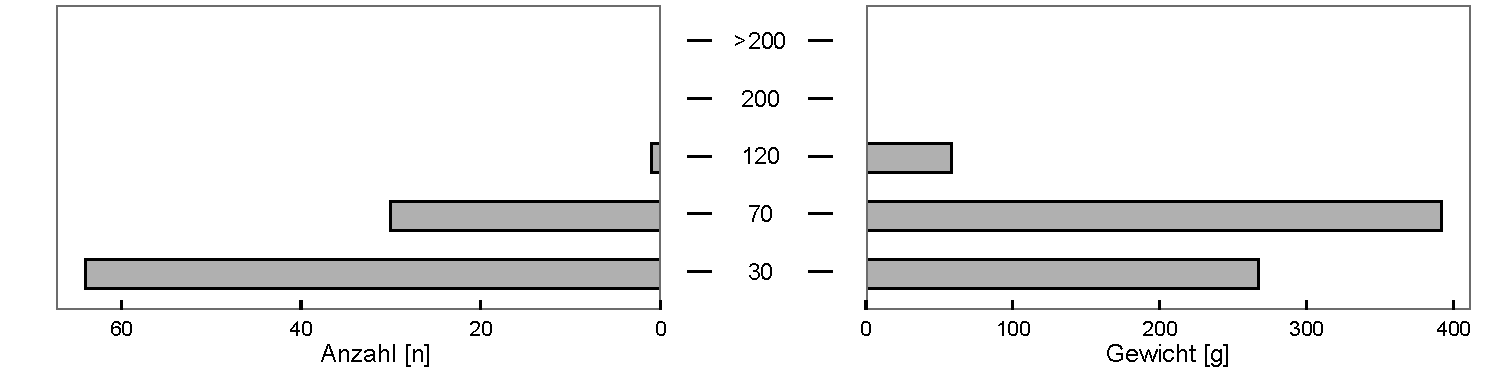
\includegraphics[width=\textwidth]{fig/9-7_BBS87-2_Fragmentierung_2.pdf}
	\caption{BBS~87/2: Fragmentierungsgrad der Scherben  (n~=~95; Größenklassen siehe Anm.~\ref{ftn:Keramik_Fragmentierung}).}
	\label{fig:Fragmenierung_BBS87-2}
\end{figure*}

Bei etwa 0,7\,m unter der Oberfläche (Abb.~\ref{fig:BBS87-2_T89Skizze}) wurde eine grob Nord--Süd-verlaufende Reihe aus fünf Stangenlöchern freigelegt. Die Stangen lagen etwa 0,2--0,3\,m auseinander und hatten einen Durchmesser von 0,6--0,8\,cm. Ihre Verfüllung bestand aus lockerem und dunklerem Substrat. Im Süd-Profil ist ein Pfostenloch (Abb.~\ref{fig:BBS87-2_T89Skizze}, \ref{fig:BBS87-2_Profile}:A) angeschnitten worden. Vor dem West-Profil wurde ein Profilsockel zur Untersuchung eines weiteren Pfostenloches (Abb.~\ref{fig:BBS87-2_T89Skizze}, \ref{fig:BBS87-2_Profile}:B) stehen gelassen. Die Richtung der Pfostenreihe deckt sich mit der Grenze der Schichten~3 und 4 aus dem zweiten Planum (Abb.~\ref{fig:BBS87-2_T76Skizze}--C). Schicht 3, die Verfüllung der wannenartigen, 0,1--0,15\,m mächtigen Vertiefung innerhalb von Schicht~4, teilt die Fläche in zwei Bereiche, deren Grenze sich im Verlauf der Pfostenreihe spiegelt. Dies lässt es naheliegend erscheinen, dass die Wand eines Gebäudes erfasst wurde. Aufgrund des kleines Aufschlusses -- von lediglich 1\,$\times$\,1\,m -- kann nicht sicher gesagt werden, welche der beiden Bereiche die potenzielle \textit{Innen}- beziehungsweise \textit{Außen}-Seite widerspiegelt.\footnote{In Bolondo am Tshuapa sind die Gebäude leicht erhaben auf Plattformen aus Lehm errichtet \parencite[369--376]{Wotzka.1995} . Diese erinnern an den durch Schicht~4 in Bobusa freigelegten Befund. Schicht~3 kann potenziell als wandparalleler, flacher Graben gedeutet werden.}

\noindent Die Grabung erbrachte den folgenden stratigrafischen Befund (Abb.~\ref{fig:BBS87-2_GrubeVorGrabung_OstProfil}; \ref{fig:BBS87-2_Profile}):
\begin{itemize}[leftmargin=*, labelindent=1em, noitemsep, topsep=0pt]
\item [(1)] \textit{Deckschicht}; mittel-/dunkelbraun; keine Funde; \textasciitilde0,15--0,2\,m mächtig
\item [(2)] dunkler als (1); keine Funde; \textasciitilde0,2--0,25\,m mächtig
\item [(3)] mittelbraun, heller als (2) beziehungsweise wie (1); zieht wannenartig in (4); wenige Funde und Holzkohle; \textasciitilde0,15\,m mächtig
\item [(4)] gelber Lehm, durchzogen von roten und dunklen Linsen; an der Basis von Schicht~4 sehr feine tonig-aschige Lagen; im östlichen Teil \textless\,0,1\,m mächtig, im westlichen Teil \textgreater\,0,3\,m mächtig
\item [(5)] mittelbraun; dunkel; homogen; schluffig--tonig; enthält viel Keramik und Holzkohle
\item [(6)] gelber anstehender Lehm
\end{itemize}

\paragraph{Keramik\vspace{.5em}}\mbox{}\\
\begin{tabular}{@{}lrl@{}}
Ausgezählt: & 328\,g & \\ 
Bearbeitet: & 342\,g & (51\,\%) \\ 
Insgesamt: & 670\,g & \\ 
\end{tabular} 

\begin{figure*}[p]
	\centering
	\begin{subfigure}[t]{\textwidth}
		\centering
		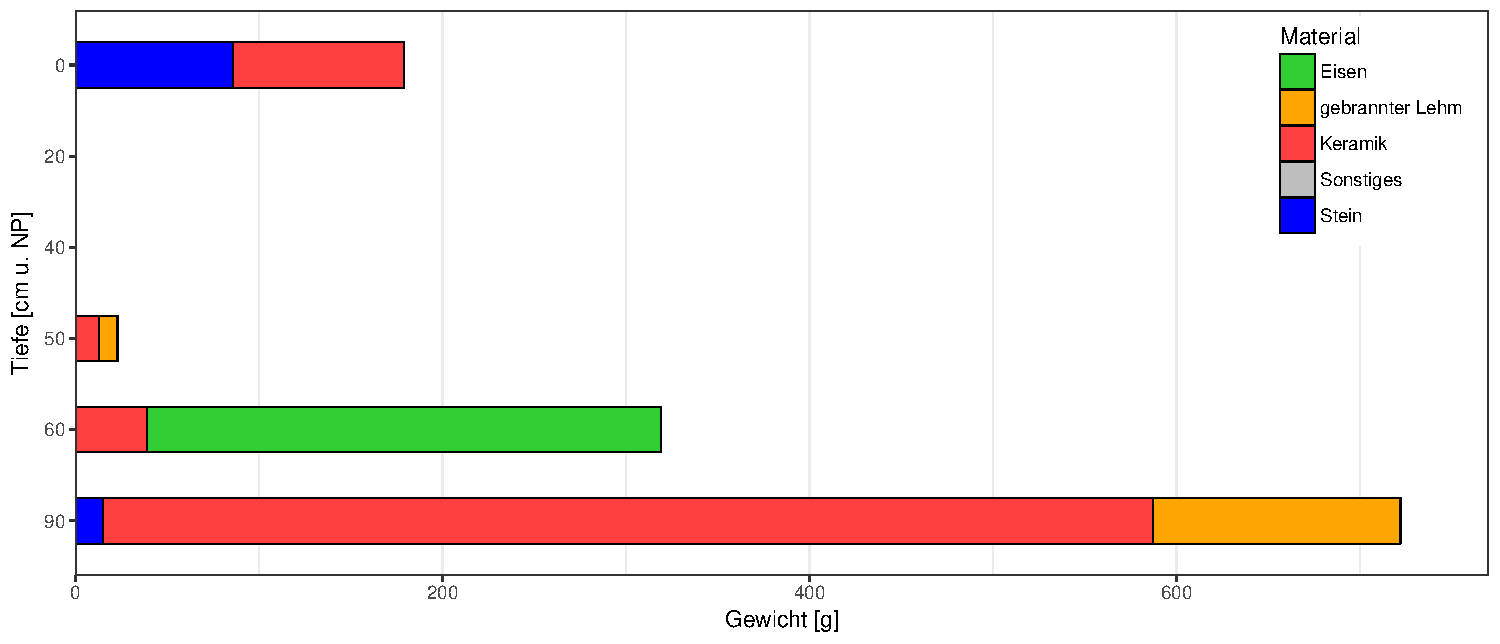
\includegraphics[width=\textwidth]{fig/9-7_BBS87-2_VerteilungFunde_R.pdf}
		\caption{Fundmaterial.\vspace{1em}}
		\label{fig:BBS87-2_VerteilungFunde}
	\end{subfigure}
	\begin{subfigure}[t]{\textwidth}
		\centering
		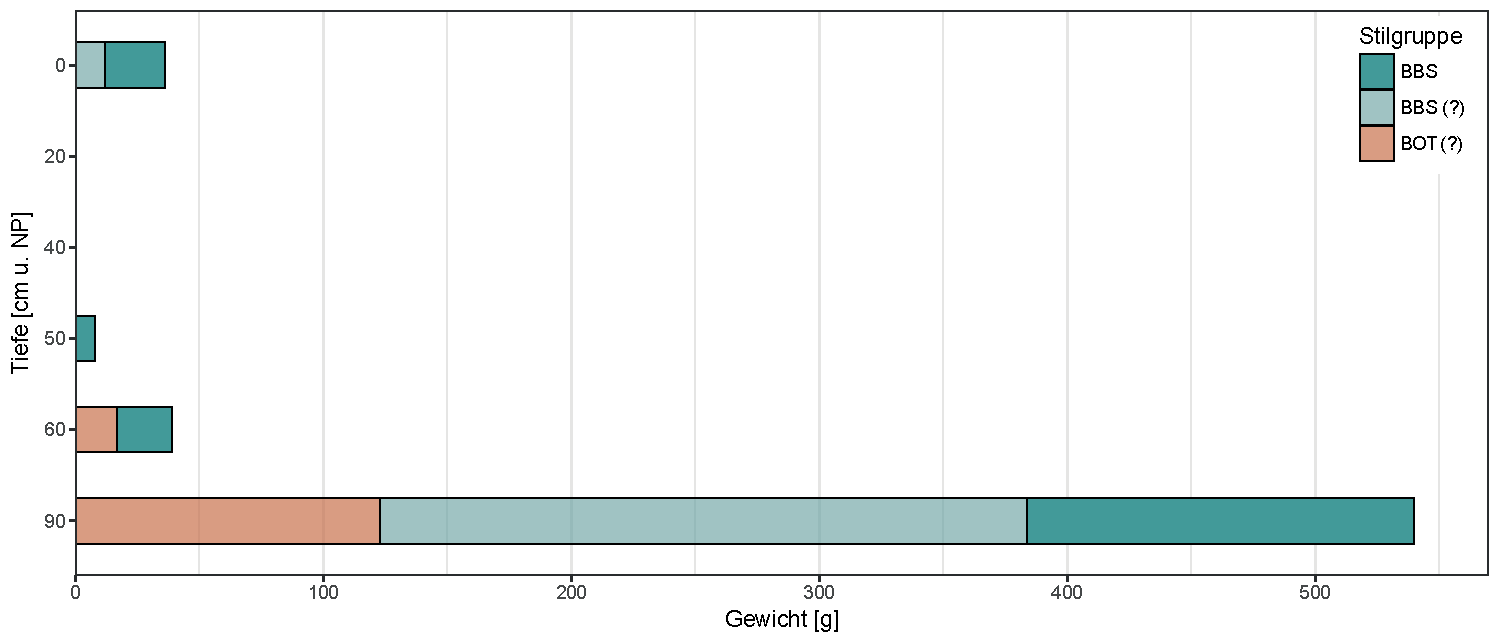
\includegraphics[width=\textwidth]{fig/9-7_BBS87-2_KeramikStilgruppen_R.pdf}
		\caption{Keramische Stilgruppen.\vspace{1em}}
		\label{fig:BBS87-2_VerteilungStilgr}
	\end{subfigure}
	\begin{subfigure}[t]{\textwidth}
		\centering
		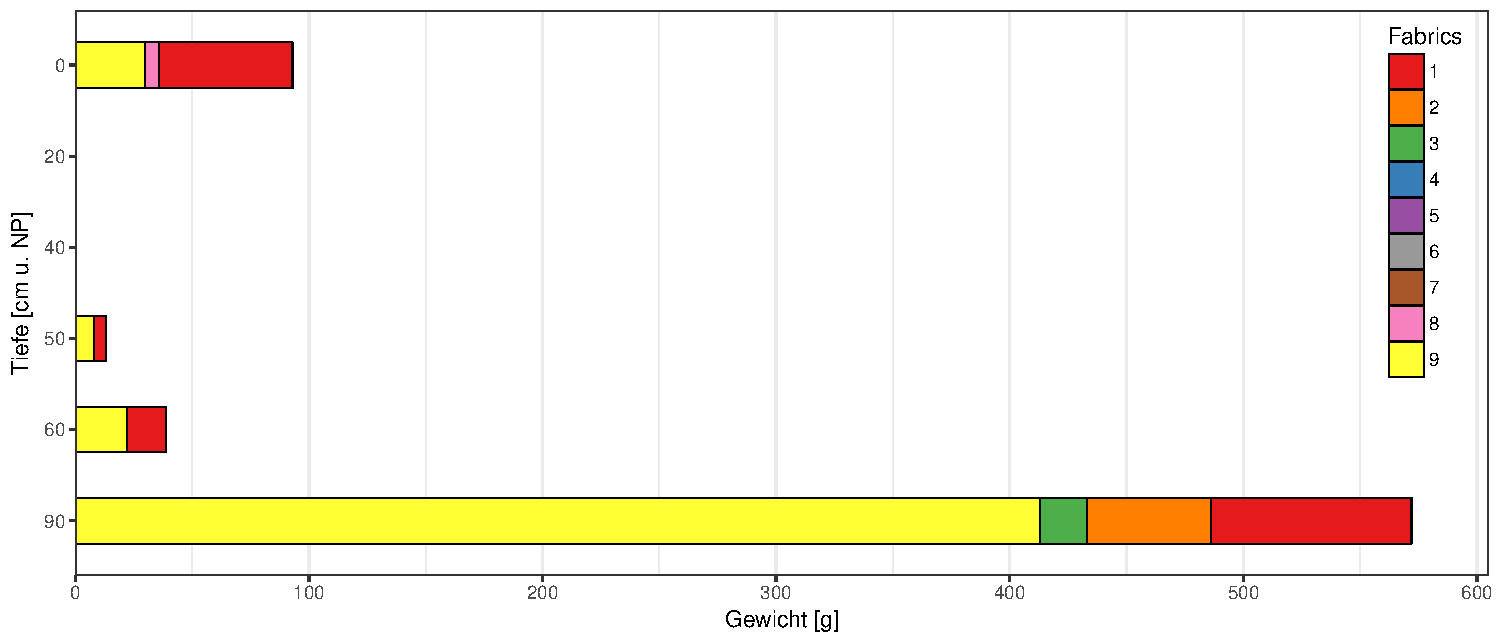
\includegraphics[width=\textwidth]{fig/9-7_BBS87-2_Fabrics_R.pdf}
		\caption{\textit{Fabrics}.}
		\label{fig:BBS87-2_VerteilungFabrics}
	\end{subfigure}
	\caption{BBS 87/2: Verteilung der Fundmaterialien (A), keramischen Stilgruppen (B) und \textit{Fabrics} (C) in den entsprechenden Tiefen der Grabung.}
	\label{fig:BBS87_2_Funde}
\end{figure*}

\vspace{1em}
\noindent Die Keramik aus der Grabung ist stark fragmentiert, Oberflächen der Scherben sind stark erodiert und Bruchkanten deutlich verrundet. Lediglich eine potenziell dem Botendo-Stil (Kap.~\ref{sec:BOT-Gr}) zurechenbare Randscherbe aus Schicht~5 ist größer als 70\,$\times$\,70\,mm. Die übrigen Scherben sind kleiner, wobei Stücke unterhalb von 30\,$\times$\,30\,mm überwiegen (Abb.~\ref{fig:Fragmenierung_BBS87-2}). Häufig sind Fragmente gerade ausbiegender Ränder mit spitzen Mündungen. Ein Teil der Scherben weist zwar formale Ähnlichkeiten zu den Stilen Botendo (Kap.~\ref{sec:BOT-Gr}) sowie Mobaka (Kap.~\ref{sec:MKA-Gr}) auf, unterscheidet sich aber durch regelhafte Schamott-Magerung (Abb.~\ref{fig:BBS87-2_VerteilungFabrics}) deutlich von den Vertretern dieser Stile an anderen Fundstellen. Die Keramik ist nur sehr spärlich verziert. Wenn überhaupt, so lassen sich fast ausschließlich horizontale Rillen (Tab.~\ref{tab:Verzierungselemente}: 02.1; 90\,\%) beobachten. Nur an jeweils einer GE ließ sich \textit{banfwa-nfwa} (Tab.~\ref{tab:Verzierungselemente}: 08) oder ein Winkelband (Tab.~\ref{tab:Verzierungselemente}: 01.6) beobachten.

Vertreter des Botendo-Stils fanden sich in großer Anzahl im Oberflächenmaterial aus dem \textit{elali}\footnote{\label{ftn:elali}Dorfwüstungen werden als \textit{bilali}; im Singular \textit{elali} bezeichnet.} (BBS~87/102), während das wenige Material aus dem Dorf (BBS~87/101) eher den Formen der Bobusa-Gruppe entspricht (Kap.~\ref{sec:BBS-Gr}).

\paragraph{Sonstige Funde}\hspace{-.5em}|\hspace{.5em}%
Im südlichen Teil des Schnitts, direkt an der Grenze von Schicht~3 und 4 fand sich etwa 0,5\,m unter der Oberfläche ein Messingdraht, bei dem es sich höchstwahrscheinlich um ein Stück \textit{Mitako}-Geld\footnote{Siehe R. K. \textcite{Eggert.1980a}.} handeln könnte (Abb.~\ref{fig:BBS87-2_T76Skizze}). Der Draht ist 72\,mm lang und hat einen Durchmesser von 4\,mm.

\begin{Figure}
	\centering
	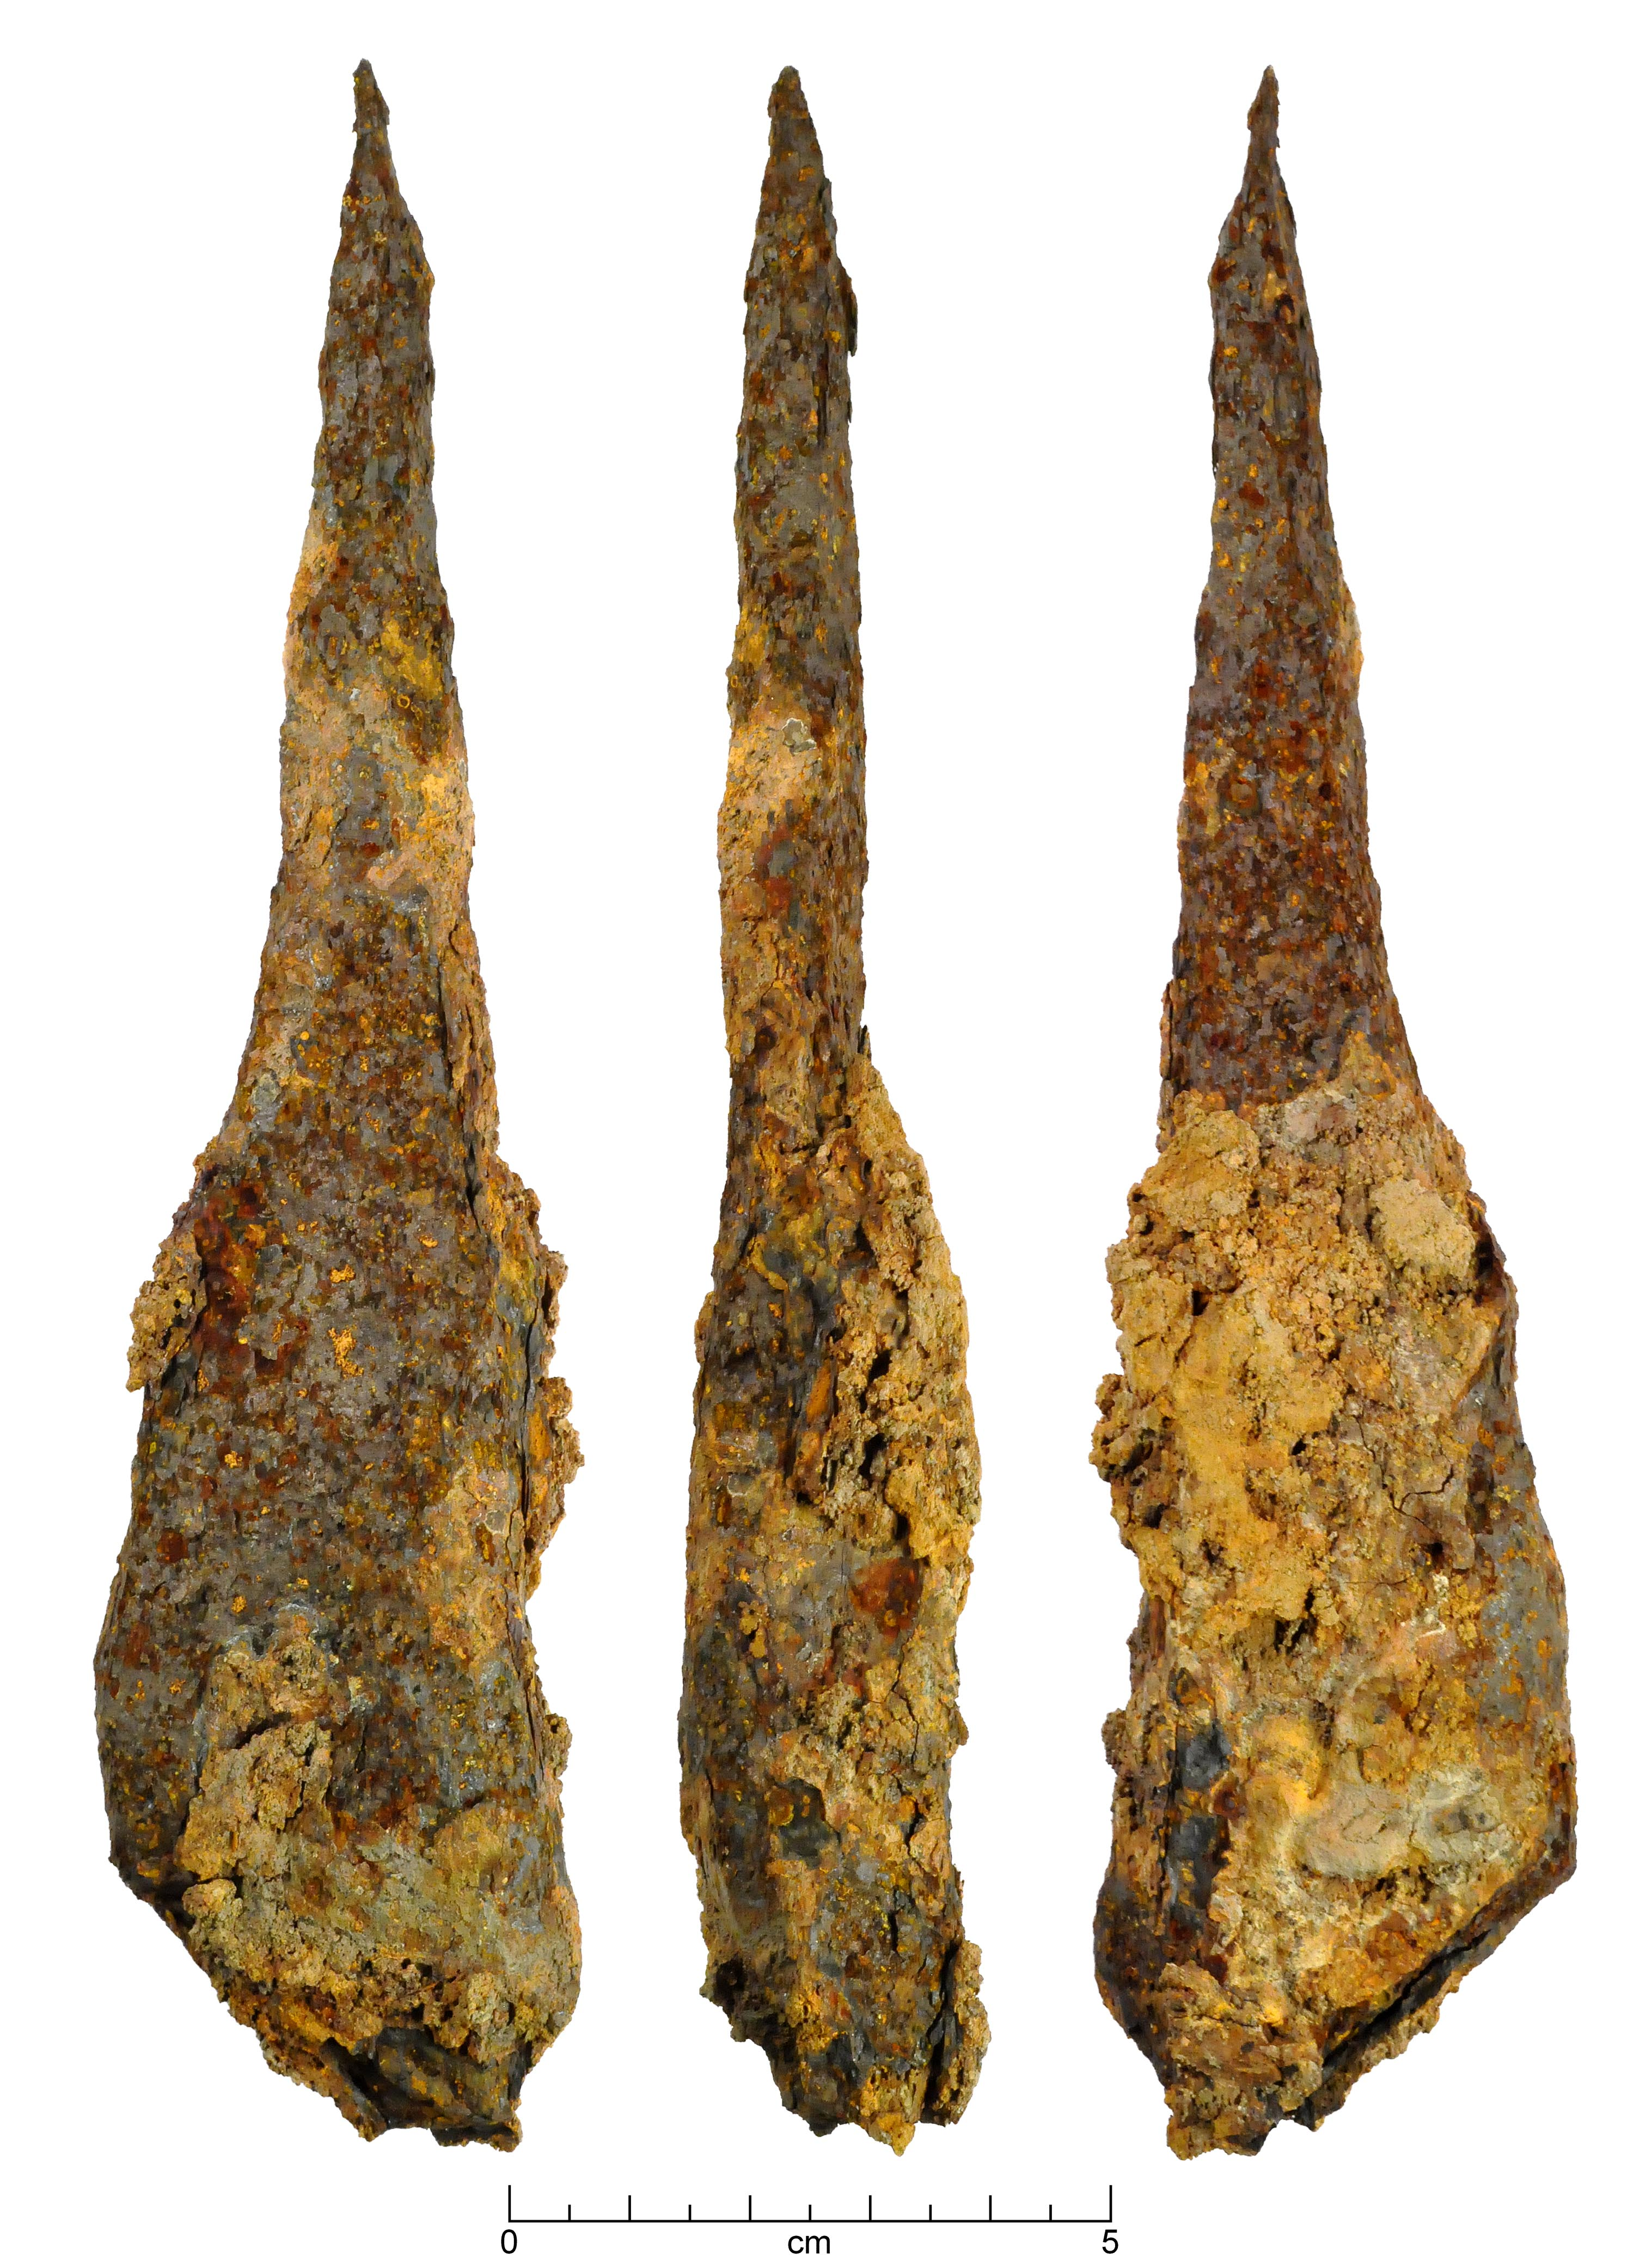
\includegraphics[width=.95\columnwidth]{fig/BBS87-2-4_Eisenspitze.jpg}
	\captionof{figure}{BBS 87/2: Eisenspitze (Foto: D. Seidensticker, 2014)}
	\label{fig:BBS87-2_Eisenspitze}
\end{Figure}

Kurz vor dem Nordprofil fand sich etwa 0,6\,m unter der Oberfläche eine Eisenspitze (Abb.~\ref{fig:BBS87-2_T83Skizze}, \ref{fig:BBS87-2_Eisenspitze}). Sie lag mit der Spitze nach Westen im gelben Lehm der Schicht~4. Die sehr massive Spitze ist 173\,mm lang, 39\,mm breit und 21\,mm hoch und hat einen rechteckigen Querschnitt. Sie weist keine Spuren einer Schäftung auf und aufgrund ihres massiven Charakters kann auch eine potenzielle Funktion als \textit{Barren} nicht ausgeschlossen werden.

\paragraph{Datierung}\hspace{-.5em}|\hspace{.5em}%
Aus der Grabung liegen keine Radiokohlenstoffdatierungen vor. Anhand der keramischen Inventare der einzelnen Schichten und Abträge lassen sich keine chronologischen Schlüsse ableiten. Lediglich die im vierten Abtrag aufgeschlossene Schicht 5 enthielt ein umfangreiches Fundinventar, das sich ausschließlich aus Vertretern der Stilgruppen Bobusa (Kap.~\ref{sec:BBS-Gr}) und Botendo (Kap.~\ref{sec:BOT-Gr}) zusammensetzt (Abb.~\ref{fig:BBS87-2_VerteilungStilgr}). Während die Botendo-Keramik frühestens in das 17.~Jh. n.~Chr. datiert werden kann \parencite[157\,f.]{Wotzka.1995}, lassen sich keine gesicherten Angaben zur Datierung der Bobusa-Keramik machen.

\paragraph{Interpretation}\hspace{-.5em}|\hspace{.5em}%
Der Testschnitt BBS~87/2 deckte unter anderem eine Feuerstelle oberhalb einer etwa 20\,cm mächtigen, fundreichen \textit{Kulturschicht} (Schicht~5) auf. Über der Feuerstelle fand sich ein zirka 0,5\,m mächtiges, fast fundfreies Paket. Des Weiteren wurde eine Nord--Süd-verlaufende Stangenreihe, die potenziell die Wand eines Gebäudes repräsentiert, freigelegt. Die Grenzen einer oberhalb dieser liegenden, flachen Eintiefung verläuft in gleicher Ausrichtung wie die Stangenreihe. Eine Zuordnung der erfassten Stangenlöcher zu einem Wohnhaus lässt sich auf dieser Basis wahrscheinlich machen.\footnote{Die traditionelle Bauweise mit dünnen Stangen und Flechtwerk lässt sich an dem Gebäude direkt neben der Grabung beobachten (Abb.~\ref{fig:BBS87-2_GrubeVorGrabung}).}

\section*{\begin{tabular*}{\linewidth}{@{}l @{\extracolsep{\fill}} r@{}}
Nr.~8 & PIK~87/1 \\
\end{tabular*} 
}

\textsf{\textbf{Pikunda (\mbox{Sangha}; Fpl.~255)}}

\vspace{1em}

\noindent\begin{tabular}{@{}rl@{}}
\textbf{Feldarbeit:} & \begin{tabular}[t]{@{}l@{}}\textbf{03.06.--13.06.1987}\\ \textbf{(M. K. H. Eggert)}\end{tabular} \\ 
\textbf{Abb.:} & \textbf{\ref{fig:PIK87_Fundstelle}--\ref{fig:PIK87_Datierungen}} \\ 
\textbf{Tab.:} & \textbf{\ref{tab:PIK87-1_Befunde}--\ref{tab:PIK87-1_Datierungen}}\\
\textbf{Taf.:} & \textbf{44.3--48.16} \\ 
\textbf{Lit.:} & \textbf{\textsc{Eggert}~1992, 1993} \\ 
\end{tabular} 

\begin{figure*}[tb]
 \centering
 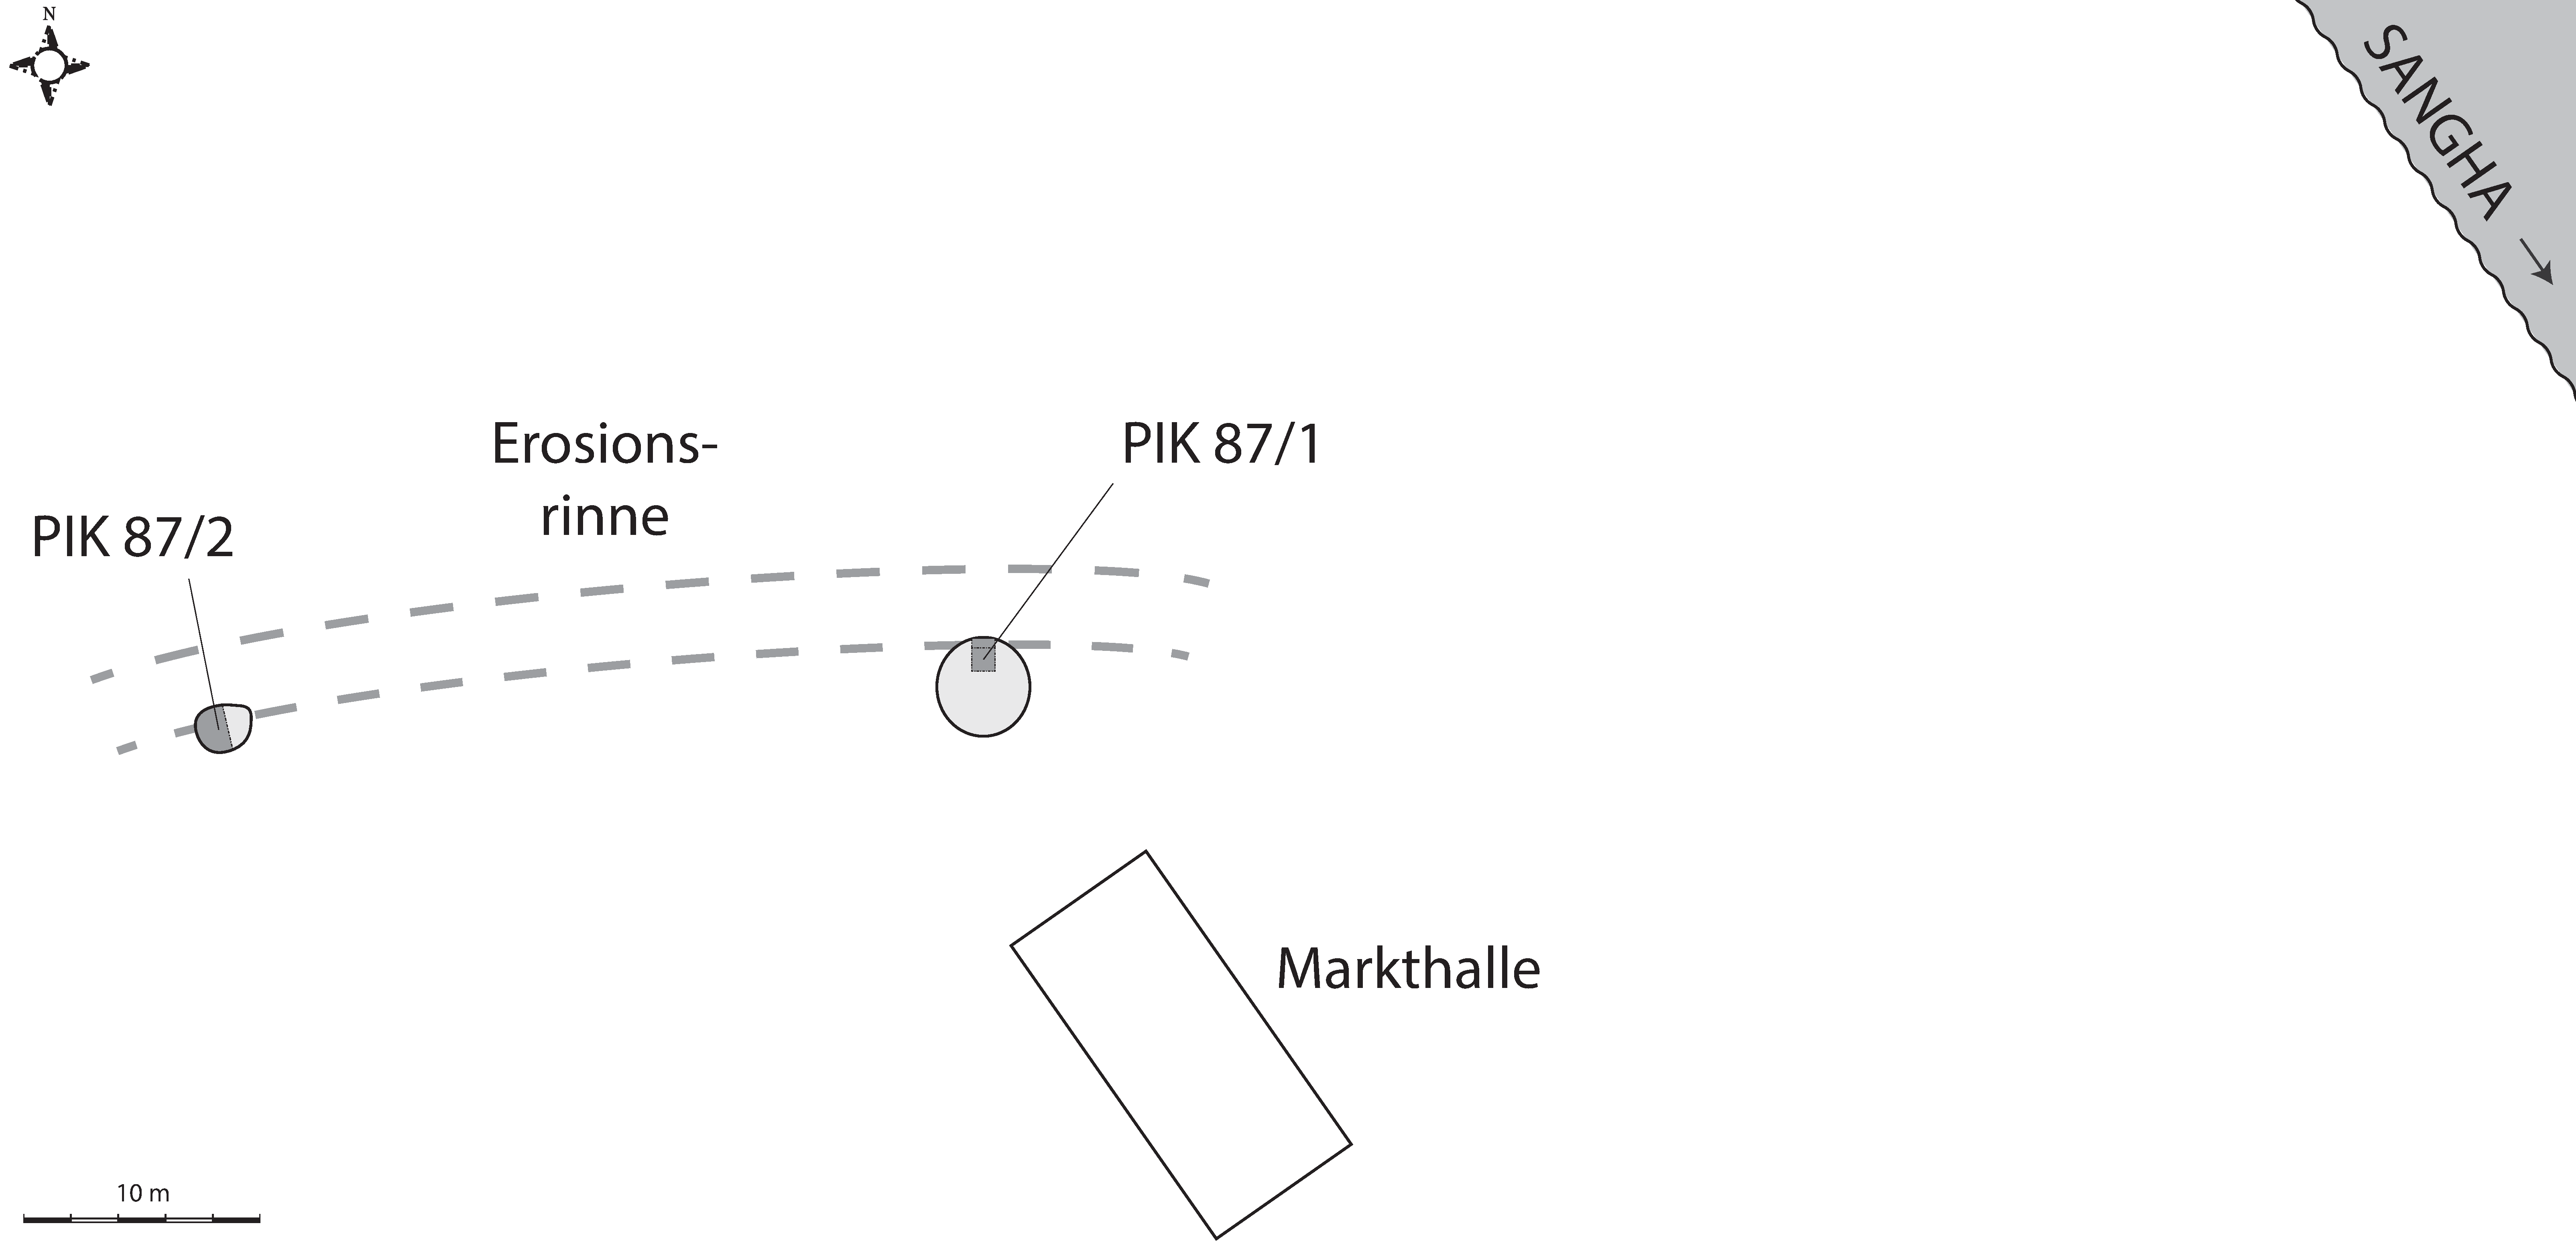
\includegraphics[width=\textwidth]{fig/PIK87_Uebersicht_2014-01-20.pdf}
 \caption{Pikunda (Fpl.~255): Grobe Lage der Grabungsstellen PIK~87/1 und PIK~87/2 (Kat.-Nr.~8--9; dunkelgrau: ausgegrabene Flächen).}
 \label{fig:PIK87_Fundstelle}
\end{figure*}

\begin{figure*}[!tb]
\centering
\begin{subfigure}[b]{\columnwidth}
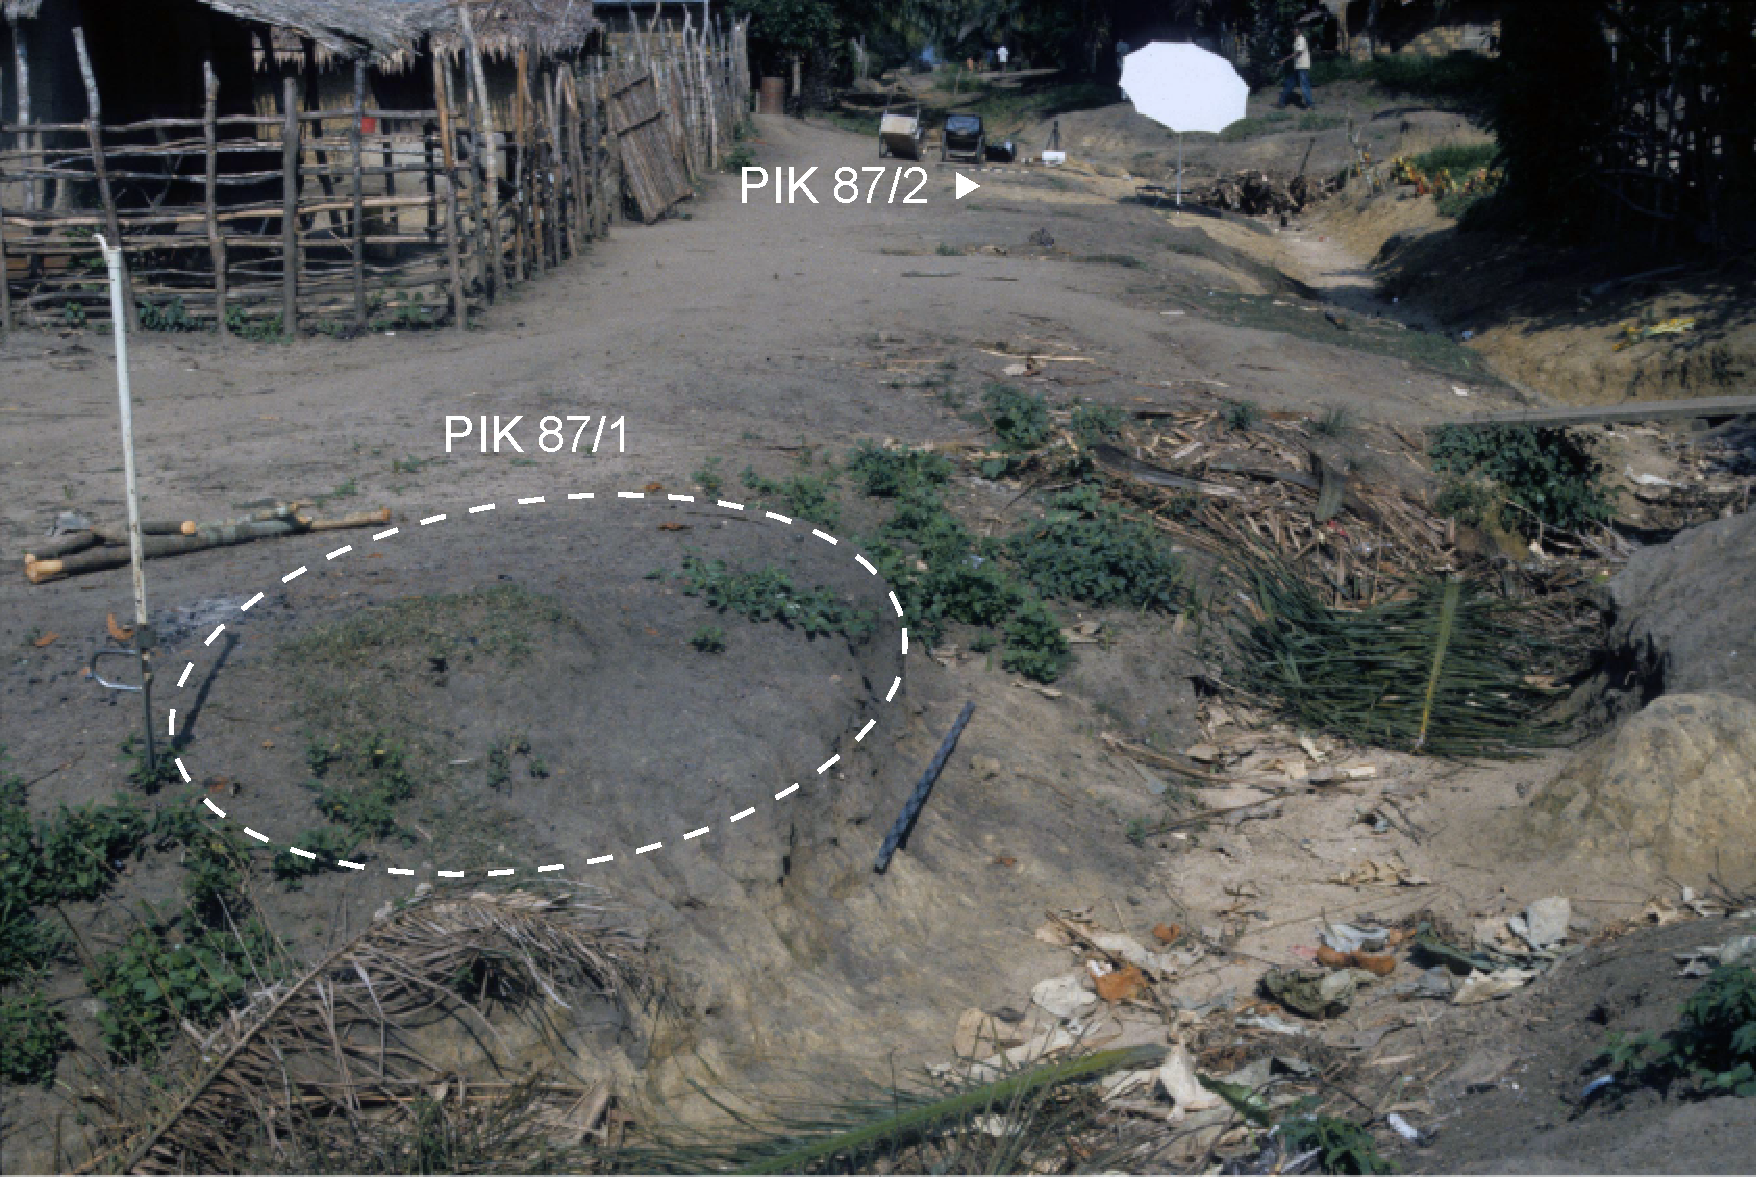
\includegraphics[width = \textwidth]{fig/PIK87-1_E87-014-6.pdf}
\caption{Übersicht von Nordwest.}
 \label{fig:PIK87-1_FundstelleObfl_vonNO}
\end{subfigure}\hfill
\begin{subfigure}[b]{\columnwidth}
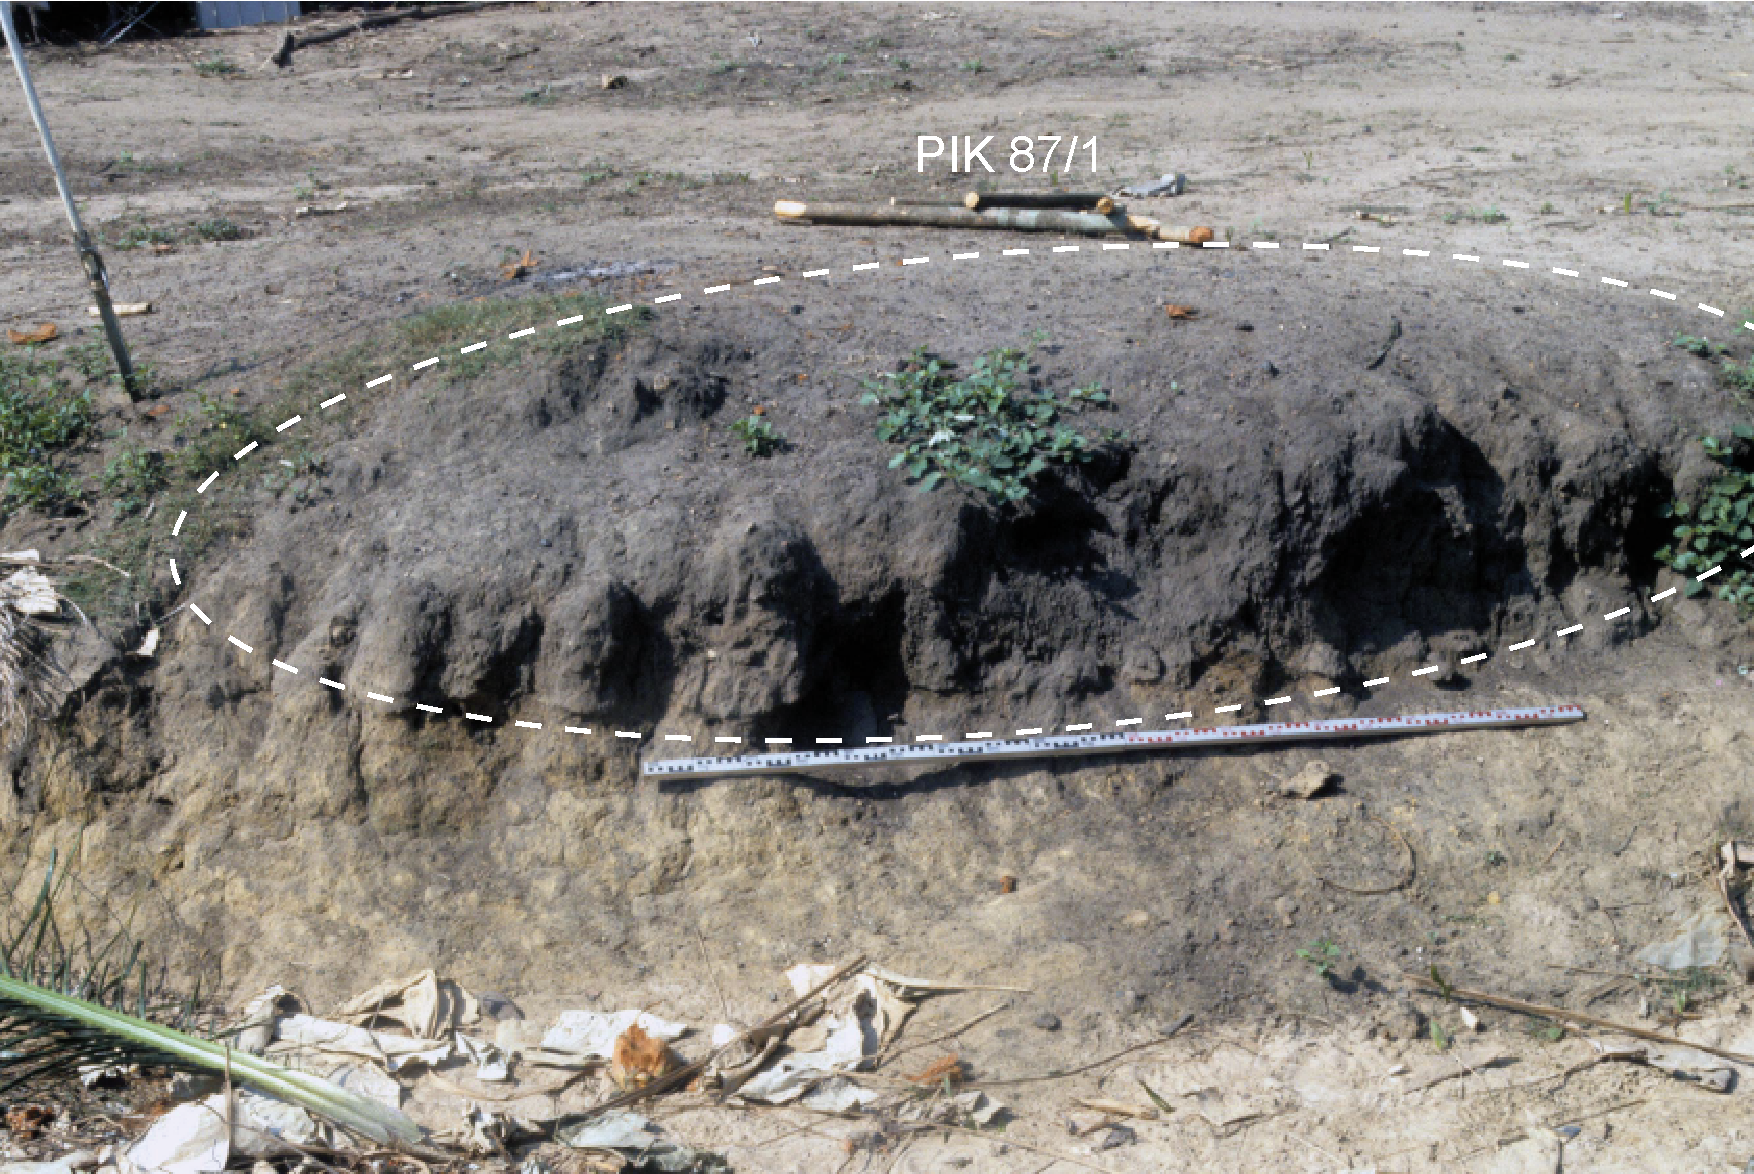
\includegraphics[width = \textwidth]{fig/PIK87-1_E87-014-3.pdf}
\caption{Blick von Nord.}
 \label{fig:PIK87-1_FundstelleObfl_vonN}
\end{subfigure}
 \caption{PIK~87/1: Grabungsstelle vor der Ausgrabung (Fotos: M. K. H. Eggert, 1987).}
 \label{fig:PIK87-1_FundstelleObfl_Foto}
\end{figure*}

\paragraph{Grabung und Befunde}\hspace{-.5em}|\hspace{.5em}%
In einer Erosionsrinne wurden bei einer ersten Prospektion am 12.\,05.\,1987 zwei teilweise freierodierte Gruben entdeckt (Kat.-Nr.~8--9). Im näheren Umfeld wurden drei Eisen-Verhüttungsöfen (\textsc{Kanimba Misago} 1995), von denen einer später unter der Kennung PIK~87/3 (Kat.-Nr.~10) untersucht wurde, und eine Reihe teilweise freierodierte Körperbestattungen gefunden. Neben Keramikscherben fand sich auch auffallend viel Eisenschlacke in diesem Bereich des Dorfes. Nach Abschluss der Prospektion entlang der Flüsse \mbox{Sangha} und \mbox{Ngoko} wurden die drei genannten Befunde systematisch ausgegraben. Die beiden Gruben liegen etwa 60\,m (PIK~87/1) beziehungsweise 90\,m (PIK~87/2) vom Ufer des \mbox{Sangha} entfernt (Abb.~\ref{fig:PIK87_Fundstelle}).\footnote{Die Lage des Verhüttungsplatzes PIK~87/3 (Kat.-Nr.~10) wurde weder beschrieben noch eingemessen und die Dokumentation des Ausgräbers C. Kanimba Misago liegt nicht vor.} Sie waren an der südlichen Kante einer nahezu Ost--West-verlaufenden, 4,5--5,5\,m breiten und 1,0--1,5\,m tiefen Rinne durch Erosion teilweise aufgeschlossen.

Die Grabungsstelle PIK~87/1 wurde zur Untersuchung einer etwa 4\,m großen, rundlichen, dunklen Verfärbung, die am östlichen Ende der Erosionsrinne beobachtet wurde, angelegt (Abb.~\ref{fig:PIK87_Fundstelle}, \ref{fig:PIK87-1_FundstelleObfl_Foto}).\footnote{Die Verfärbung war in O--W-Richtung 4\,m breit und vom Südende bis zum im Zuge der Grabung angelegten Nord-Profil waren es 3,8\,m (Abb.~\ref{fig:PIK87-1_PlanaSkizze}). Der Abstand zwischen dem Nord-Profil und der nördlichen Grubengrenze wurde nicht gemessen. Auf einigen Situationsfotos, die nach einem starken Regenschauer aufgenommen wurden, ist die Ausdehnung der dunklen Verfärbung deutlich zu sehen.} Die Grabung erfasste einen Teil des nördlichen Abschnitts dieser Verfärbung. Zu Beginn wurde ein etwa Ost--West-orientiertes, der Kante der Erosionsrinne folgendes Profil angelegt und der zügig abgetiefte Profilkasten als PIK~87/1/I bezeichnet (Abb.~\ref{fig:PIK87-1_PlanaSkizze}, \ref{fig:PIK87-1_ProfileFotos}).\footnote{Das bis auf etwa 3\,m unter die Oberfläche abgetiefte Profil diente vor allem der Bestimmung der Tiefe der die Verfärbung bildenden Befunde. Während des Aushebens des Profilkastens wurde nur wenig Keramik und kaum Holzkole gefunden. Teile eines Gefäßes fanden sich zwischen 1,65--1,75\,m unter der Oberfläche (Abb.~\ref{fig:PIK87-1_ProfileZeichnung}; Taf.~44.3). Weitere einzelne Scherben fanden sich zwischen 2,20--2,80\,m unter der Oberfläche. Erst ab etwa 2,80\,m, im Bereich der Sohle von Grube B1/B2, fand sich deutlich mehr Holzkohle sowie einige Brocken gebrannten Lehms.} Südlich an dieses Profil anschließend wurde eine 1\,$\times$\,1\,m große Fläche in 15 künstlichen, jeweils 20\,cm mächtigen Abträgen ausgegraben.\footnote{Eine Dokumentation von dabei angelegten Plana erfolgte nicht.} Durch die Grabung wurden zwei Gruben erfasst, die im Weiteren als Befund A und B bezeichnet werden. Die tiefere und ältere Grube B wird von einer jüngeren Grube A geschnitten (Abb.~\ref{fig:PIK87-1_ProfileZeichnung}, \ref{fig:PIK87-1_ProfileFotos}).\footnote{Obwohl während der Grabung keine Trennung des Fundmaterials aus diesen beiden Befunden erfolgte, lässt sich das Fundinventar eindeutig in zwei Komplexe unterteilen, die mit dem stratigrafischen Befund korrespondieren (Abb.~\ref{fig:PIK87-1_VerteilungStilgr}--D).}

\begin{figure*}[tb]
 \centering
 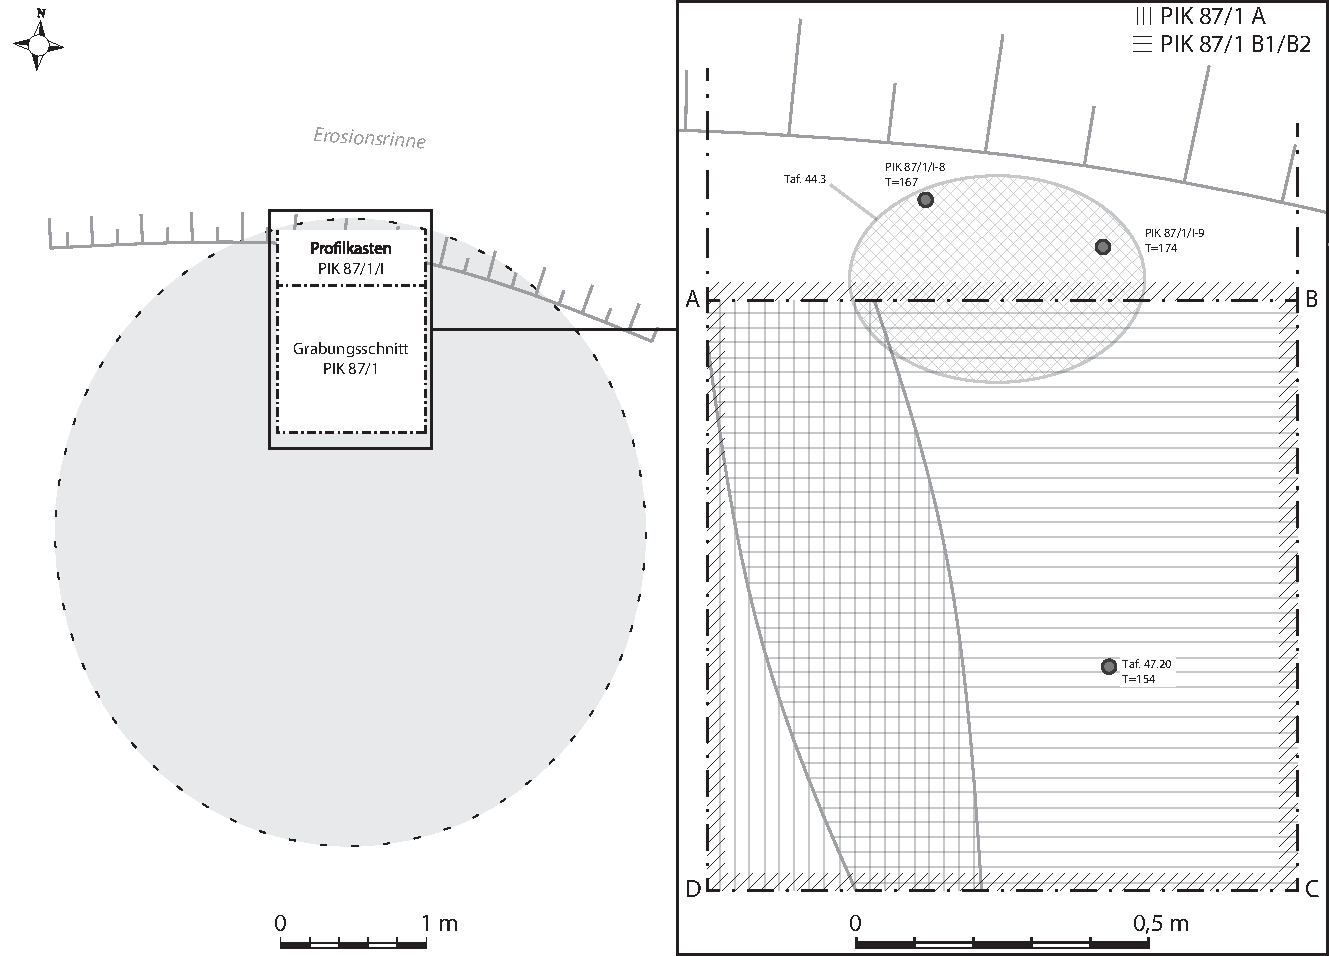
\includegraphics[width=\textwidth]{fig/PIK87-1_Planum_Keramik.pdf}
 \caption{PIK~87/1: Planskizze mit Positionsangaben zu eingemessenen Einzelfunden und summarische Rekonstruktion der Befundsituation im Planum (rechts).}
 \label{fig:PIK87-1_PlanaSkizze}
\end{figure*}

\begin{figure*}[p]
\centering
\begin{subfigure}[t]{\columnwidth}
 \centering
 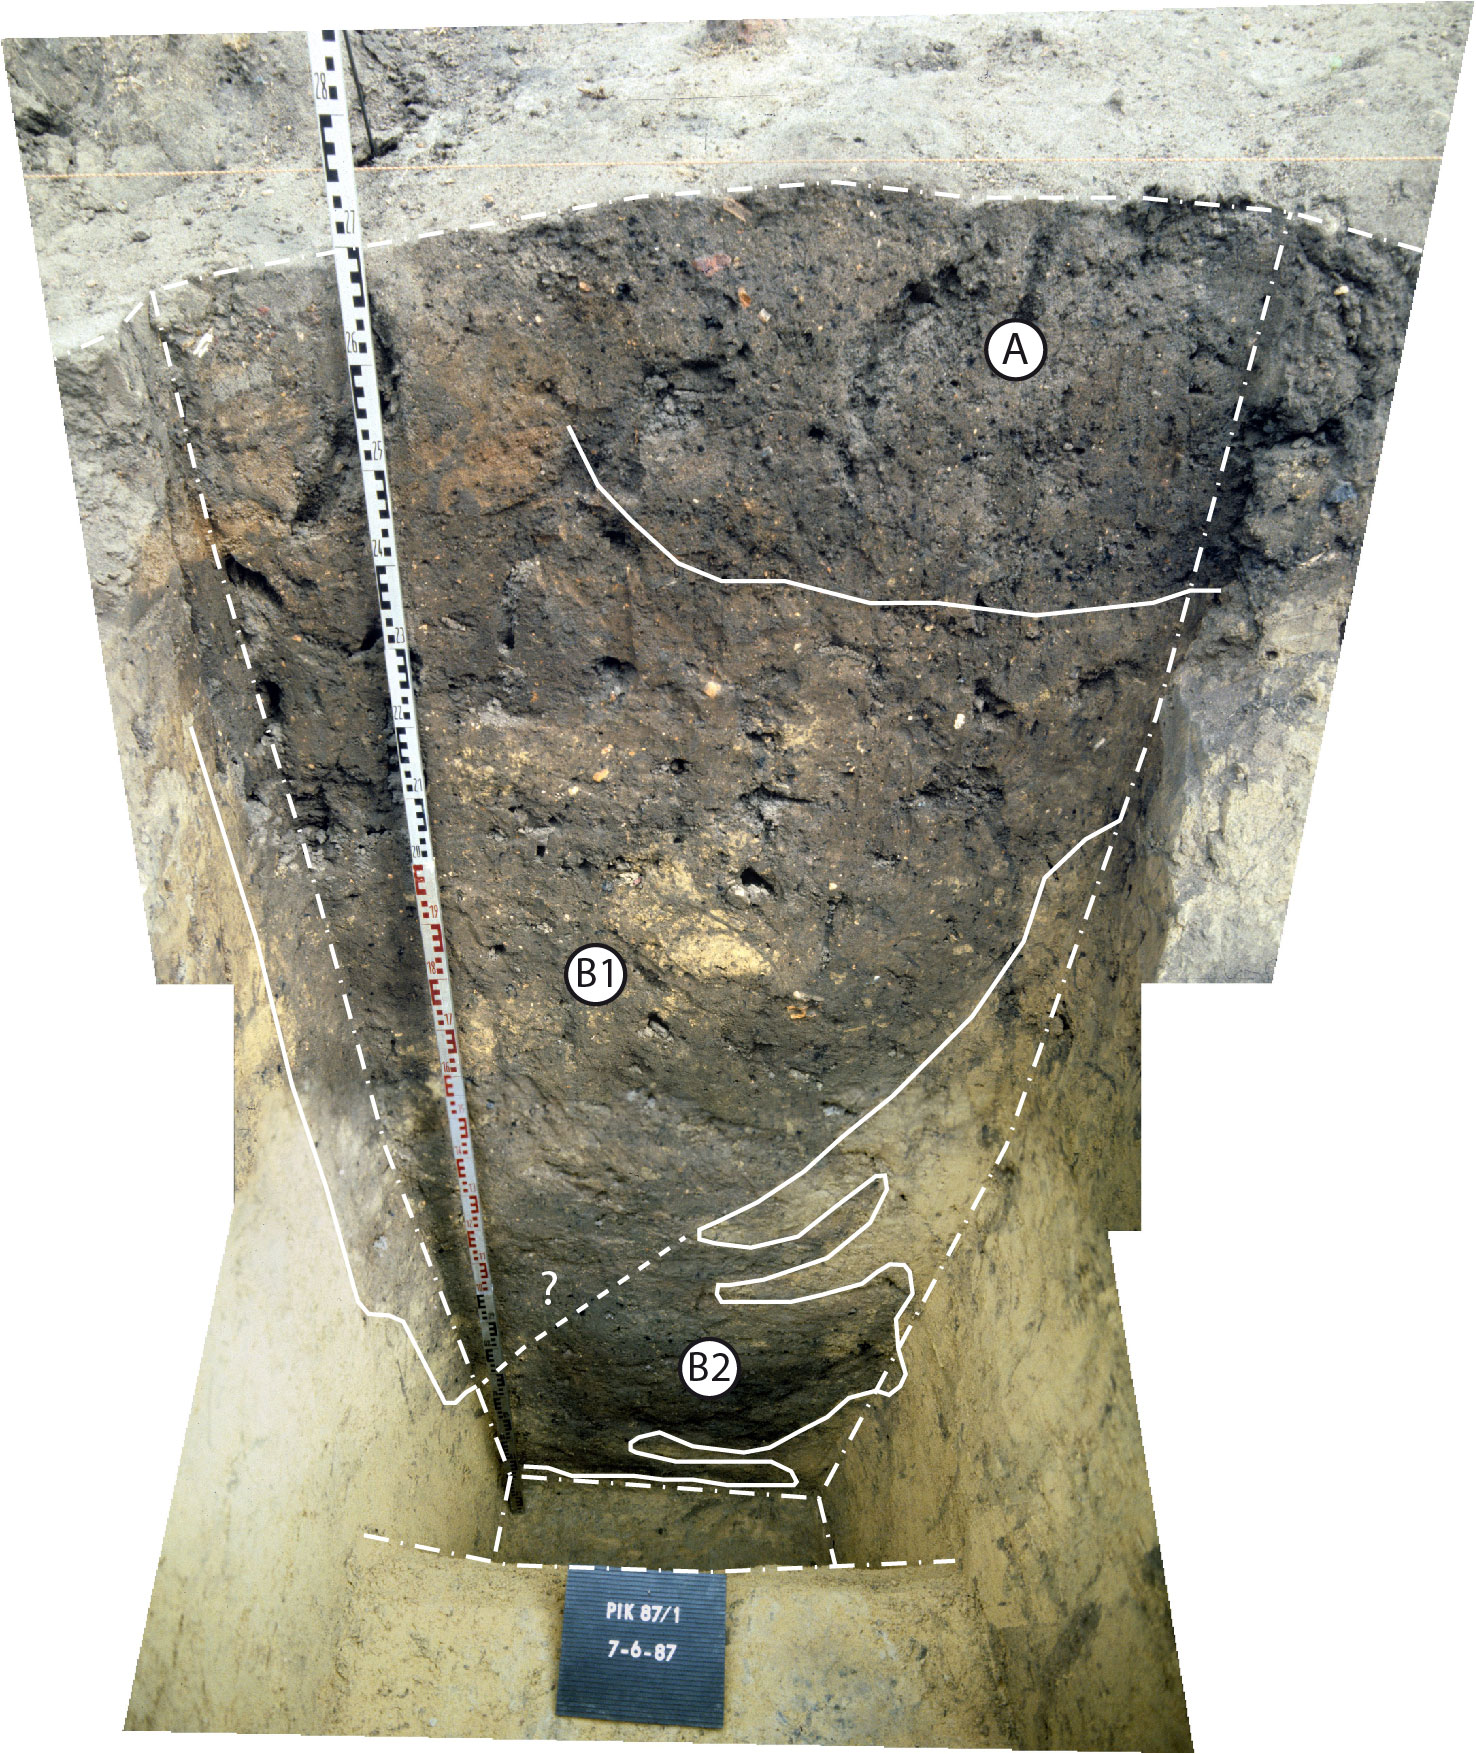
\includegraphics[width=\columnwidth]{fig/PIK87-1_N-profil_E87-018-26--28-01_2014-01-01.jpg}
 \caption{Nord-Profil}
 \label{fig:PIK87-1_N-Prof}
\end{subfigure}\hfill
\begin{subfigure}[t]{\columnwidth}	
 \centering
 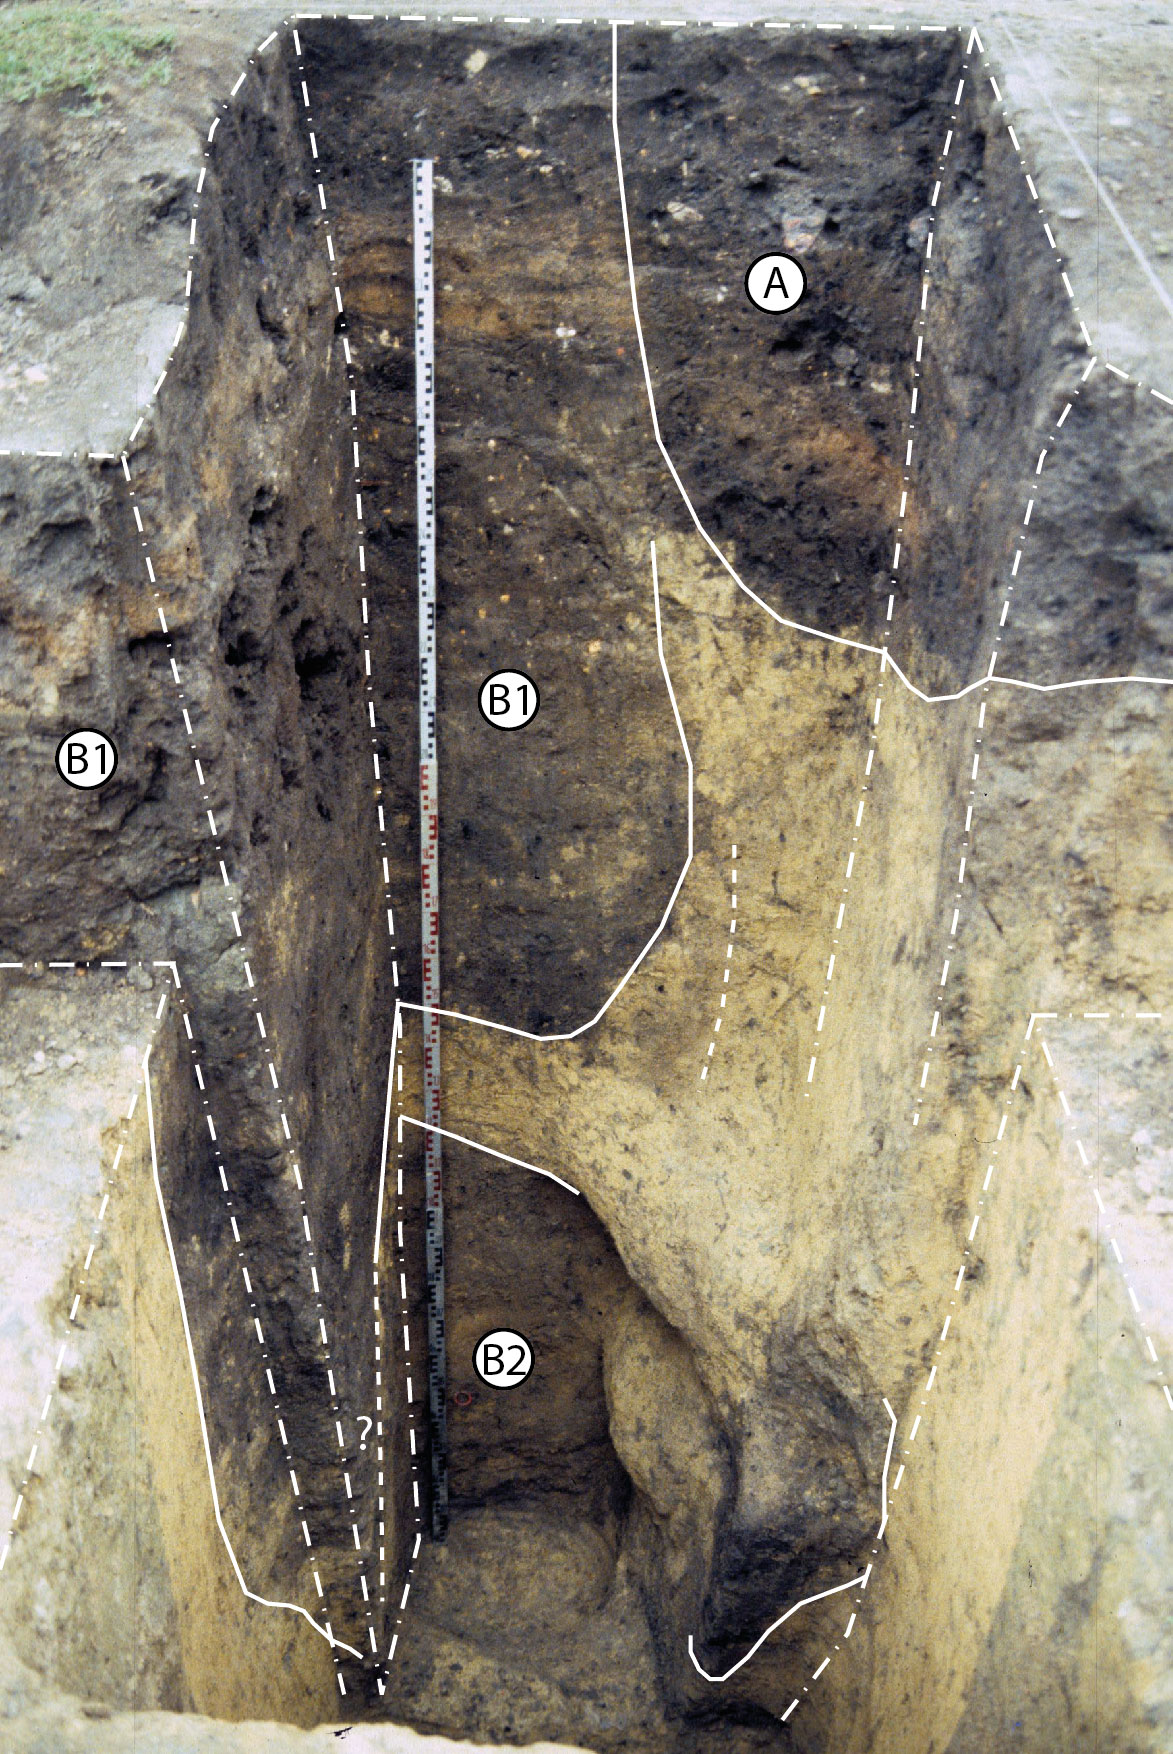
\includegraphics[width=.8\columnwidth]{fig/PIK87-1_S-Profil_E87-020-2_2014-01-01.jpg}
 \caption{Grabungsschnitt mit Ost-, Süd- und West-Profil}
 \label{fig:PIK87-1_O+S+W-Prof}
\end{subfigure}
 \caption{PIK~87/1: Profile (Fotos: M.~K.~H. Eggert, 1987).}
 \label{fig:PIK87-1_ProfileFotos}
\end{figure*}

\begin{figure*}[p]
	\centering
	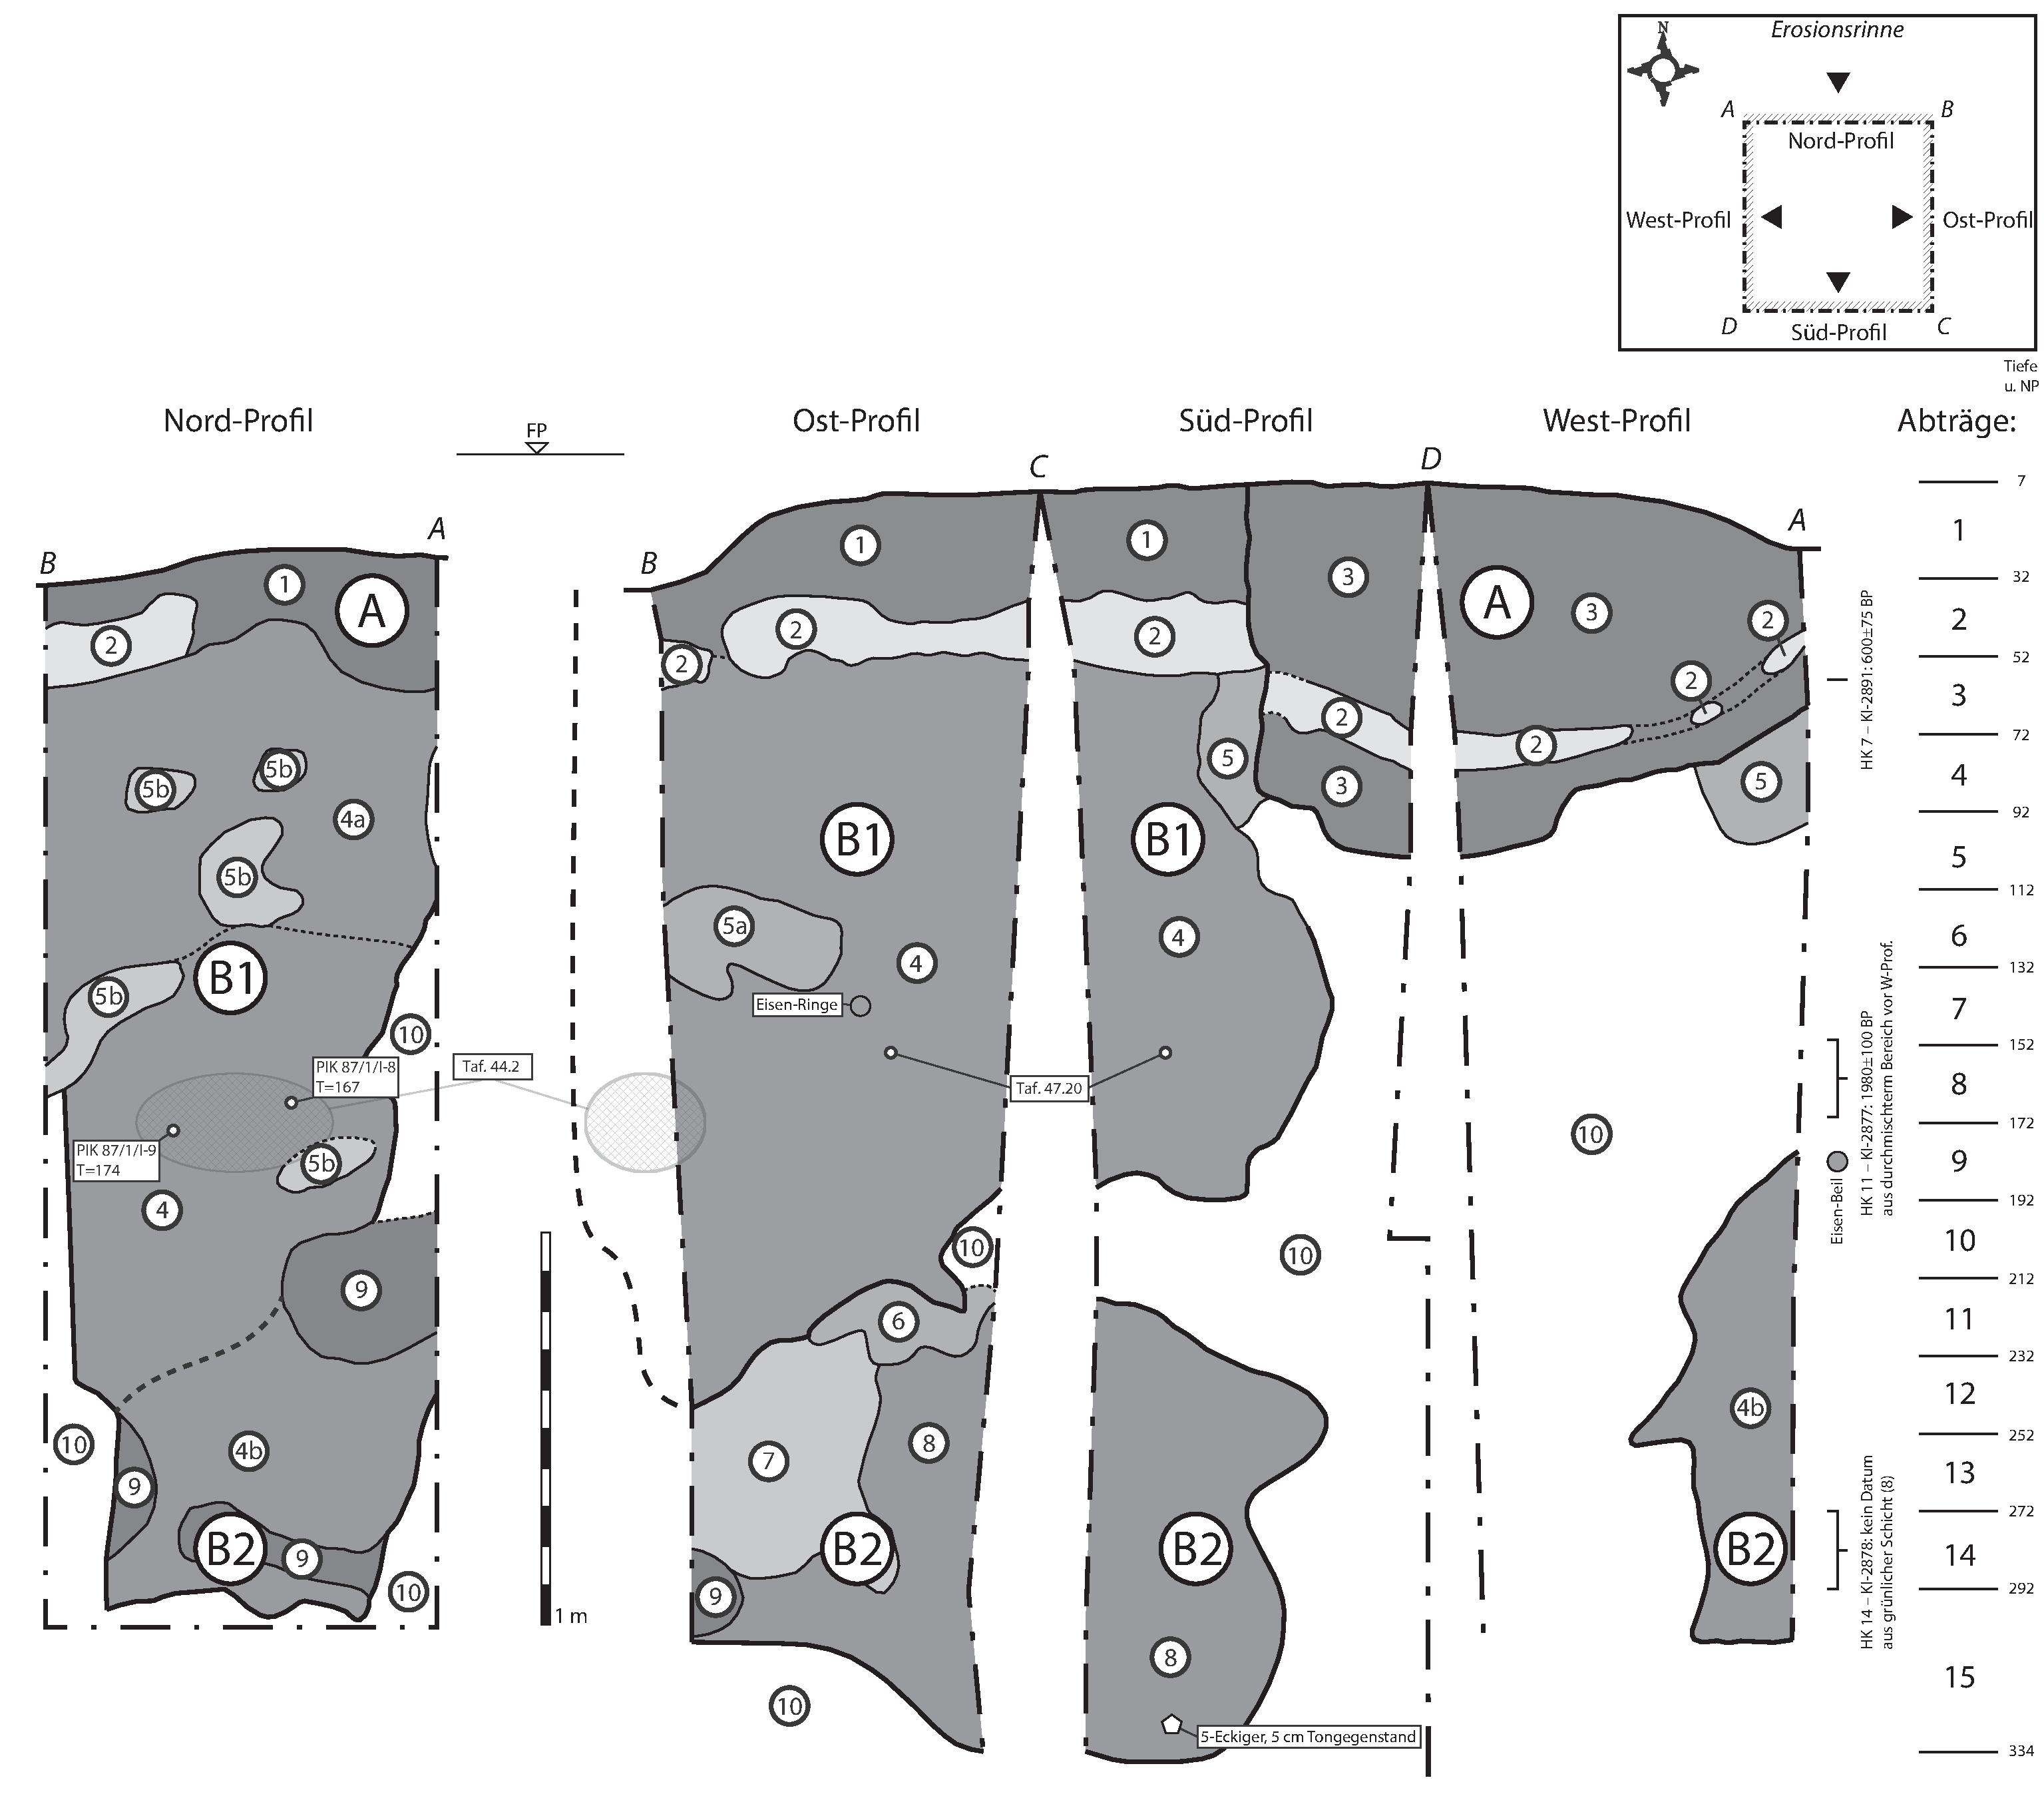
\includegraphics[width=.9\textwidth]{fig/PIK87-1.pdf}
	\caption{PIK~87/1: Profile.}
	\label{fig:PIK87-1_ProfileZeichnung}
\end{figure*}

Die bis 0,95\,m unter die heutige Oberfläche reichende Grube A wurde im südwestlichen und westlichen Teil des Schnittes erfasst (Abb.~\ref{fig:PIK87-1_ProfileZeichnung}). Der Befund greift in den oberen Bereich der Grube B1/B2 ein und ist folglich stratigrafisch jünger (Abb.~\ref{fig:PIK87-1_ProfileFotos}). Die Wandung von Grube A ist vertikal bis steilschräg, ihre Sohle konvex und die Ecken gerundet bis fließend. Da die Begrenzung des Befundes lediglich im Süd-Profil erfasst wurde, können keine sicheren Angaben zum Durchmesser der Grube gemacht werden (Abb.~\ref{fig:PIK87-1_ProfileZeichnung}).\footnote{Der bei der Grabung erfasste Teil von Grube A entspricht grob einem Volumen von 0,3\,m\textsuperscript{3}. Im Westprofil war die nördliche Grenze der Grube bereits durch Erosion abgetragen. Unter der Annahme, dass in nördlicher Richtung ein eher fließenderer Übergang von Sohle und Wandung vorlag und die bei Profilnagel D erfasste Tiefe der tiefste Punkt des Befundes ist, würde die nördliche Begrenzung etwa 30--40\,cm über die Erosionsrinne hinausragen. Auf Basis dieser Annahmen und dem Schnittpunkt der Grube im Westprofil ließe sich ein Durchmesser von etwa 2,6\,m rekonstruieren. Mit einem solchen Durchmesser würde eine runde Grube allerdings 0,5--1,0\,m über die maximale Ausdehnung der an der Oberfläche sichtbaren Verfärbung hinausreichen. Eventuell ist daher mit einer eher ovalen Form der Grube A zu rechnen.} Auffällig ist die rötliche Schicht~2, die etwa 0,3--0,4\,m unterhalb der rezenten Oberfläche horizontal durch beide Befunde verläuft. In Grube A ist diese Schicht allerdings um etwa 0,2--0,3\,m nach unten versetzt und befindet sie sich in einer Tiefe von etwa 0,5--0,7\,m unter der Oberfläche (Abb.~\ref{fig:PIK87-1_ProfileZeichnung}).\footnote{Ob es sich bei dem Material der Schicht 2 um einen Teil des Aushubs handelt, der später wieder mit verfüllt wurde, muss offenbleiben, kann aber als wahrscheinlich angenommen werden.}

Die stratigraphisch ältere Grube B lässt sich in zwei Bereiche untergliedern. Der obere Teil B1 reicht bis mindestens 2,7\,m unter die heutige Oberfläche. Die Verfüll-Schichten~4 und 4a sind homogen mittel- bis dunkelbraun und weisen teilweise hellere Einschlüsse auf, die Schichten~5a und 5b. Im Südprofil wurde die vertikale bis leicht konvexe Grubenwandung bis zu einer Tiefe von etwa 1,8\,m unter der heutigen Oberfläche, beziehungsweise 0,9\,m oberhalb der Sohle des unteren Bereichs B2 erfasst. Die Unterkante des Abschnitts B1 fällt schräg, mit etwa 30$^\circ$ Neigung nach Nordosten ab. Der tiefste erfasste Punkt dieses oberen Bereiches liegt im Bereich von Nagel B (Abb.~\ref{fig:PIK87-1_PlanaSkizze}, \ref{fig:PIK87-1_O+S+W-Prof}, \ref{fig:PIK87-1_ProfileZeichnung}).\footnote{Die nördliche Grubenwandung liegt etwa 0,2--0,3\,m nördlich des Nord-Profils (Abb.~\ref{fig:PIK87-1_O+S+W-Prof}, \ref{fig:PIK87-1_ProfileFotos}, \ref{fig:PIK87-1_ProfileZeichnung}).} Unterhalb des Verfüllpaketes B1 befindet sich ein weiteres, B2 genanntes Paket, das im westlichen Bereich teilweise vom anstehenden Lehm (Schicht 10) überlagert wird. Die Verfüllung dieses Bereiches (Schichten~4b und 6--9) ist heterogener als der obere Teil B1. Es sind deutlich häufiger gelbe, lehmige Linsen beziehungsweise Einschlüsse zu beobachten und grundsätzlich ist das Substrat etwa heller, als das des oberen Bereiches. Schicht~8 wird zudem als leicht grünlich beschrieben. Sie enthielt den Großteil, der nur noch eher spärlichen Keramik aus diesem Abschnitt. An der Sohle fanden sich keine bis kaum Funde, aber weiterhin sehr viel Holzkohle. Der Grubenteil B2 wurde bis etwa 3,25\,m unter die heutige Oberfläche nachvollzogen. Ab dieser Tiefe fanden sich kleine Laterit-Knollen.

%\vspace{1.5em}
\columnbreak
\noindent Die Grabung erbrachte den folgenden stratigrafischen Befund (Abb.~\ref{fig:PIK87-1_ProfileZeichnung}):
\begin{itemize}[leftmargin=*, labelindent=1.25em, noitemsep, topsep=0pt]
\item [(1)] 10 YR 3/1 bis 10 YR 3/1.5; Sand (S)
\item [(2)] 10 YR 4.5/5; Sand (S) mit dunklerem Boden (etwa 2.5 Y 3/2)
\item [(3)] 10 YR 3/2; toniger Sand (tS); mehr Holzkohle als in den anderen Schichten
\item [(4)] 10 YR 3.5/3; toniger Lehm (tL)
\item [(4a)] 10 YR 3/2; toniger Lehm (tL)
\item [(4b)] 10 YR 3.5/2; toniger Lehm (tL)
\item [(5)] 10 YR 3/3; schluffiger Lehm (uL); heterogen gelblich
\item [(5a)] 10 YR 3/3 mit 10 YR 6/5; sandiger Ton (sT)
\item [(5b)] 10 YR 4/3; durchmischt mit 10 YR 6/6, lehmig
\item [(6)] 10 YR 3/3; schluffiger Lehm (uL)
\item [(7)] 10 YR 6/3.5 bis 2.5 Y 6/3; toniger Lehm (tL)
\item [(8)] 2.5 Y 4/2; grünlich; lehmiger Schluff (lU); teils auch etwas mit Gelb durchmischt
\item [(9)] 2.5Y 4/4 bis 10 YR 3.5/3 bis 10 YR 6/6; toniger Lehm (tL)
\item [(10)] 10 YR 6/6; toniger Lehm (tL)
\end{itemize}

\begin{table*}[tb]
	\vspace{2em}
	\centering
	%{\footnotesize \begin{sftabular}{@{}p{.1\textwidth}p{.1\textwidth}p{.15\textwidth}p{.15\textwidth}p{.4\textwidth}@{}}
	{\footnotesize \begin{sftabular}{@{}lllrll@{}}\toprule 
			\textbf{Grube} & \textbf{Bereich} & \textbf{Abträge} & \textbf{Tiefe} & \textbf{Schichten} & \textbf{keramische Stilgruppen} \\ 
			\midrule 
			A & & 1--5 & 0--1,03\,m & 3 & Mandombe (Ebambe, Matoto, Konda, Pandama, Mbenja) \\ 
			\multirow{2}{*}{B} & 1 & 1--12 & 0--2,34\,m & 4, 4a, 5a, 5b & Pikunda-Munda (\mbox{Ngbanja} und evtl. Lusako) \\ 
			& 2 & 9--15 & 2,10--3,36\,m & 4b, 6, 7, 8, 9 & Pikunda-Munda (evtl. Lusako) \\ 
			\bottomrule 
	\end{sftabular}}
	\caption{PIK~87/1: Erfasste Gruben.}
	\label{tab:PIK87-1_Befunde}
\end{table*}

\begin{table*}[tb]
	\centering
	{\footnotesize \begin{sftabular}{@{}lrrrr@{}}
\toprule
   \textbf{Fundkategorie} &  \textbf{Anzahl} &    \textbf{\%} &  \textbf{Gewicht (kg)} &    \textbf{\%} \\
\midrule
           Eisen &       3 &   0,4 &          0,06 &   0,2 \\
 gebrannter Lehm &       9 &   1,3 &          0,09 &   0,3 \\
         Keramik &     462 &  67,3 &         23,28 &  79,9 \\
         Knochen &       9 &   1,3 &          0,25 &   0,9 \\
        Ofenwand &       4 &   0,6 &          0,03 &   0,1 \\
        Schlacke &     162 &  23,6 &          4,88 &  16,7 \\
          Sonder &       3 &   0,4 &          0,01 &   0,0 \\
           Stein &      32 &   4,7 &          0,53 &   1,8 \\
          Tuyère &       2 &   0,3 &          0,01 &   0,0 \\
\bottomrule
\end{sftabular}
}
	\caption{PIK~87/1: Anteil verschiedener Fundmaterialien.}
	\label{tab:PIK87-1_Funde}
\end{table*}

\paragraph{Keramik\vspace{.5em}}\mbox{}\\
\begin{tabular}{@{}lrl@{}}
	Ausgesondert: & 11\,300\,g & \textit{40\,\% glatte Wandung} \\
	& & \textit{60\,\% rauwandig} \\
	Ausgezählt: & 2886\,g & \\
	Bearbeitet: & 9137\,g & (76\,\%) \textit{ohne 1987} \\
	& & \textit{ausgesondertes Material} \\
	Insgesamt: & 23\,323\,g &
\end{tabular}

\vspace{1em}
\noindent 
Die durch die Grabung erfassten Funde zeichnet die geschilderte Befundsituation und Unterschiede der beiden erfassten Gruben nach (Abb.~\ref{fig:PIK87-1_VerteilungFunde}). Das Gros -- zirka 78\,\% -- aller Funde fand sich in den hauptsächlich mit der Grube A zu assoziierenden, obersten vier Abträgen.\footnote{Im Zuge der Reinigung und Durchsicht der Funde am Ende der Feldkampagne von 1987 wurden im Materiallager in Bamanya etwa 50\,\% der aus der Grabung PIK~87/1 stammenden Keramik als \textit{nicht diagnostisch} ausgesondert. Die Stücke wurden in \textit{glatt}- und \textit{rau}-wandig unterschieden und nach Abträgen getrennt summarisch gewogen. Einige Scherben der beiden Gruppen wurden stellvertretend mitgenommen. Bei den Referenz-Scherben der \textit{rau}-wandigen Keramik handelt es sich durchweg um mit Schlickerrauung versehene Scherben des Mandombe-Stils (Kap.~\ref{sec:MDB-Gr}). Schlickerrauung lässt sich im untersuchten Material nur auf den unteren Hälften von Gefäßen dieser Stilgruppe beobachten. Die 1987 ausgesonderte, \textit{rau}-wandige Keramik kann unter Vorbehalt der Mandombe-Gruppe zugeordnet werden. Unter den Referenzstücken der \textit{glatt}-wandigen Keramik sind neben Stücken, die -- aufgrund ihres Scherbens (\textit{Fabric}~1) -- der Pikunda-Munda-Gruppe zugerechnet werden können, auch solche, die der Mandombe-Gruppe (\textit{Fabric}~3) zuzurechnen sind. Da oberhalb des fünften Abtrages (T~112) keramisches Material der Stilgruppen Mandombe (Grube A) und Pikunda-Munda (Grube B1) gemeinsam auftreten, ist eine Integration der 1987 ausgesonderten \textit{glatt}-wandigen Keramik oberhalb von etwa 1\,m Tiefe nicht mehr möglich. Die unterhalb dieser Tiefe ausgesonderte, \textit{glatt}-wandige Keramik kann, von vereinzelten Importstücken abgesehen, grundsätzlich nur der Pikunda-Munda-Gruppe (Kap.~\ref{sec:PKM-Gr}) zugerechnet werden. Im Material finden sich keine Scherben der Mandombe-Gruppe unterhalb des fünften Abtrages. Auffällig ist, das sich in den Abträgen 7--8 (T~152--172) auch knapp 200\,g \textit{rau}-wandige Keramik fanden. Es ist anzunehmen, das es sich dabei nicht um schlickergeraute Scherben der Mandombe-Gruppe gehandelt hat, sondern um \textit{gröbere} Keramik der \mbox{Ngbanja}-Gruppe (Kap.~\ref{sec:NGB-Gr}). Vertreter der \mbox{Ngbanja}-Gruppe finden sich in dieser Tiefe auch im aufgenommen Material (Abb.~\ref{tab:PIK87-1bis9_nichtPIK-MUN}).} Unterhalb dieses Bereiches steigt das Fundaufkommen in den Abträgen 8--9, etwa 1,8\,m unter der heutigen Oberfläche, noch einmal leicht an.\footnote{Der Anstieg des Fundaufkommens bei etwa 1,8\,m unter der Oberfläche (Abb.~\ref{fig:PIK87-1_VerteilungFunde}) ist vor allem einem fast vollständigen Gefäß (Taf.~44.3) sowie einem großen Gefäßfragment (Taf.~45.2) geschuldet.} Nichtkeramische Funde machen etwa 20\,\% des gesamten Fundgutes aus und finden sich verstärkt in den auch an Keramik reichen Abträgen.

\begin{figure*}[p]
	\centering
	\begin{subfigure}{\textwidth}	
		\centering
		\includegraphics[width = \textwidth]{fig/9-8_PIK87-1_VerteilungFunde_R.pdf}
		%\includegraphics[height = .3\textheight]{output/figs/9-8_PIK87-1-1987ausgesondert_A.pdf}
		\caption{Fundmaterial.\vspace{1em}}	
		%\caption{1987 ausgesondert}
		\label{fig:PIK87-1_VerteilungFunde}
	\end{subfigure}
	\begin{subfigure}{\textwidth}
		\centering
		\includegraphics[width = \textwidth]{fig/9-8_PIK87-1_KeramikStilgruppen_R.pdf}
		%\includegraphics[height = .3\textheight]{output/figs/9-8_PIK87-1_KeramikStilgruppen.pdf}
		\caption{Keramische Stilgruppen.\vspace{1em}}
		\label{fig:PIK87-1_VerteilungStilgr}
	\end{subfigure}
	\begin{subfigure}{\textwidth}	
		\centering
		\includegraphics[width = \textwidth]{fig/9-8_PIK87-1_Fabrics_R.pdf}
		%\includegraphics[height = .3\textheight]{output/figs/9-8_PIK87-1_Fabrics.pdf}
		\caption{\textit{Fabrics}.\vspace{1em}}
		\label{fig:PIK87-1_VerteilungFabrics}
	\end{subfigure}
	\begin{subfigure}{\textwidth}	
		\centering
		\includegraphics[width = \textwidth]{fig/9-8_PIK87-1_Schlacken_R.pdf}
		%\includegraphics[height = .3\textheight]{output/figs/9-8_PIK87-1_Fabrics.pdf}
		\caption{Schlacken.}
		\label{fig:PIK87-1_Schlacken}
	\end{subfigure}
	\caption{PIK~87/1: Verteilung der Fundmaterialien (A), keramischen Stilgruppen (B), \textit{Fabrics} (C) und Schlacken (D) in den entsprechenden Tiefen der Grabung.}
	\label{fig:PIK87-1_KeramikVerteilung}
\end{figure*}

\begin{figure*}[tb!]
	\centering
	\includegraphics[width=\textwidth]{fig/9-08_PIK87-1_Fragmentierung_2.pdf}
	\caption{PIK~87/1: Fragmentierungsgrad der Scherben (n~=~462; Größenklassen siehe Anm.~\ref{ftn:Keramik_Fragmentierung}).}
	\label{fig:PIK87-1_Fragmentierung}
\end{figure*}

Die Inventare beider Gruben zeigen eine vergleichbare Fragmentierung. Das Gros (80--90\,\%) bilden kleine bis mittelgroße Fragmente, die kleiner als 70\,$\times$\,70\,mm sind (Abb.\ref{fig:PIK87-1_Fragmentierung}). Nur in den oben bereits erwähnten Abträgen 3--4 und 8--9 fanden sich große Fragmente von Gefäßen, die größer als 120\,$\times$\,120\,mm sind. Da das Fundaufkommen nahe der Grubensohle -- dem Bereich B2 -- stark abnimmt, sind belastbare Aussagen über die Fragmentierung in dieser Zone kaum möglich. Generell ist die Funddichte in der Pikunda-Munda-Keramik-enthaltenden Grube B sehr gering. Die Verteilung der keramischen Stilgruppen spiegelt die beiden erfassten Gruben ebenfalls wider (Abb.~\ref{fig:PIK87-1_VerteilungStilgr}). Im oberen, die Abträge 1--5 umfassenden, Bereich A dominieren Gefäße mit stark geschweifter Wandung, kurzen Zylinderhälsen und ausbiegenden Rändern des Mandombe-Stils (Kap.~\ref{sec:MDB-Gr}). Erst weiter unterhalb finden sich Fragmente von Schalen mit Bauchknick des Pikunda-Munda-Stils (Kap.~\ref{sec:PKM-Gr}). 

\begin{table*}[tb]
	\centering
	{\footnotesize \begin{sftabular}{@{}lrrrrrr@{}}
			\toprule 
			\textbf{Stilgruppe} & \textbf{Gefäß} & \textbf{Rand} & \textbf{Wand} & \textbf{Boden} & \textbf{Summe} & \\ 
			\midrule 
			Mandombe & 2 & 22 & 80 & & 104 & 54,45\,\% \\ 
			fraglich Mandombe & & 46 & 29 & 3 & 78 & 40,84\,\% \\ 
			Konda & & 1 & 1 & & 2 & 1,05\,\% \\ 
			Pandama & & & 2 & & 2 & 1,05\,\% \\ 
			Ebambe & & & 1 & 1 & 2 & 1,05\,\% \\ 
			Matoto & & 2 & & & 2 & 1,05\,\% \\ 
			Mbenja & & & 1 & & 1 & 0,52\,\% \\ 
			\midrule
			Summe & 2 & 71 & 168 & 4 & 245 & \\ 
			\bottomrule 
	\end{sftabular} }
	\caption{PIK~87/1 (A): Anteil Scherben der verschiedenen Gefäßbereiche nach Stilgruppen.}
	\label{tab:PIK87-1A_Keramik_Scherben}
\end{table*}

\paragraph{Keramikinventar in Grube A\vspace{.5em}}\mbox{}\\
\begin{tabular}{@{}lr@{}}
Bearbeitet & \\ 
\hline 
Keramik der Mandombe-Gruppe: & 7056\,g \\ 
Sonstige Stilgruppen in Grube A: & 96\,g \\ 
 & \\ 
1987 Ausgesondert & \\ 
\hline 
\begin{tabular}[c]{@{}l@{}}\textit{rau}-wandige Keramik\\ (potenziell Mandombe-Gruppe)\end{tabular} & 6500\,g \\ 
\end{tabular} 		

\vspace{1em}
\noindent Die oberen Abträge erbrachten eine sehr charakteristische und formal wie technisch homogene Keramik, die als Mandombe-Stil beschrieben ist (Kap.~\ref{sec:MDB-Gr}).\footnote{Das Material aus dem Befund diente als das definierende Spektrum für die Beschreibung des Mandombe-Stils (Kap.~\ref{sec:MDB-Gr}). Um eine Verwechslung mit dem Pikunda-Munda-Stil, der von \textcite{Eggert.1992} als Keramikgruppe eingeführt wurde, zu vermeiden, wurde ein anderer, aussagefähiger Komplex für die Bennung gesucht. Entsprechende Keramik wurde in keiner anderen Grabung erfasst. Die Oberflächenabsammlung von Mandombe am \mbox{Sangha} (Fpl.~259) enthielt jedoch entsprechendes Material und wurde daher für die Benennung der Stilgruppe ausgewählt.} Sie hebt sich vom ansonsten in der Grabung freigelegten Fundspektrum deutlich ab. Keramik des Mandombe-Stils beschränkt sich auf die in den Profilen beobachtete Tiefe der Grube A und obwohl im Feld keine Trennung der Funde nach den Befunden möglich war, kann als starke Hypothese gelten, dass die Mandombe-Keramik aus Grube A stammt.

Das Inventar besteht aus 13~GE die sicher der stark bauchigen Gefäßform D1\footnote{Das Verhältnis von Bauch- zu Halsdurchmesser, welches als Maß der \textit{Bauchigkeit} gelten kann, liegt zwischen 1,5--2,6; die Werte spiegeln somit leicht bis stark bauchige Gefäße wider. Ein signifikanter Kolmogorow-Smirnow-Test unterstreicht eine zweigipfelige Verteilung, mit dezidiert schwach sowie stark bauchigen Gefäßen. Es scheint kein kontinuierliches Spektrum zwischen Gefäßen mit weniger oder solchen mit stark geschweifter Wandung zu geben. Jedoch beruht diese Beobachtung lediglich auf einer geringen Stichprobengröße.} zugeordnet werden können und 16 weiteren GE, die nicht gut genug erhalten waren, um eine eindeutige Ansprache zu ermöglichen.\footnote{Aufgrund der starken Fragmentierung (Abb.~\ref{fig:PIK87-1_Fragmentierung}) war häufig nur eine eingeschränkte Ansprache der Gefäßform möglich.} Es fanden sich keine Scherben, die einer anderen Gefäßform zugerechnet werden könnten. Ränder sind durchweg kurz und ausbiegend, mit einer gerillten Mündung und gehen in typisch kurze, zylindrische Hälse über. Die Schulterbereiche sind stark abgesetzt, häufig mit einem scharfen Knick an der Innenseite. Die Verzierungen der Keramik des Mandombe-Stils unterscheiden sich deutlich von jener der Pikunda-Munda-Keramik aus der älteren Grube B. Im ersten und zweiten Abtrag fand sich jeweils eine mit \textit{knotted strip}-Roulette (Tab.~\ref{tab:Verzierungselemente}: 21.1) verzierte Scherbe. Beide Stücke entsprechen in ihren weiteren formalen Charakteristika dem ansonsten nicht rouletteverzierten Mandombe-Material. Das früheste Auftreten von Rouletteverzierung im Arbeitsgebiet muss auf Basis dieses Fundes in das 12.--14. Jh. n. Chr. datiert werden.

Die in Grube A gemachten Funde deuten eine höhere Funddichte an, als in der älteren Grube B. In der kleineren Grube A fand sich zusammengenommen mehr Keramik, als in der etwa dreimal so tiefen Grube B. Zusätzlich enthielt die Grube noch fast 4,6\,kg Schlacke (Abb.~\ref{fig:PIK87-1_VerteilungFunde}). Das Inventar zeigt keine Anzeichen einer planmäßigen Deponierung von Objekten. Es wurden weder vollständige Gefäße gefunden, noch sind größere Zusammensetzungen möglich gewesen. Keine der in die Grube gelangten GE repräsentiert ein ganzes Gefäß.

\paragraph{Sonstige Stilgruppen in Grube A}\hspace{-.5em}|\hspace{.5em}%
Unter dem Material aus den oberen Abträgen fanden sich neben der Keramik des Mandombe-Stils einige Scherben anderer keramischer Gruppen. Diese machen weniger als 3\,\% des insgesamt der Grube A zugewiesenen Materials aus. Eine mit der für die Ebambe-Gruppe (Kap.~\ref{sec:EBA-Gr}) typischen \textit{banfwa-nfwa}-Verzierung versehene Bodenscherbe und eine entsprechend verzierte Wandungsscherbe fanden sich im zweiten Abtrag. Beide Stücke weisen keine nicht-plastischen Partikel im Scherben auf (\textit{Fabric}~1). Zudem fanden sich eine Reihe Wandungsscherben mit \textit{banfwa-nfwa}-Verzierung, die technisch der Keramik der Mandombe-Gruppe ähneln und das \textit{Fabric}~3 aufweisen.\footnote{Ob es sich bei den genannten Stücken mit \textit{Fabric}~1 um einen \textit{Import} handelt und die Scherben mit \textit{banfwa-nfwa}-Verzierung und \textit{Fabric}~3 Teil einer lokalen Produktion sind, muss gegenwärtig offenbleiben.} Darüber hinaus fanden sich vereinzelte Scherben, die Ähnlichkeiten zu den Stilen Matoto (Kap.~\ref{sec:MAT-Gr}), Konda (Kap.~\ref{sec:KON-Gr}), Pandama (Kap.~\ref{sec:PDM-Gr}) und Mbenja (Kap.~\ref{sec:MBJ-Gr}) aufweisen (Abb.~\ref{fig:PIK87-1_VerteilungStilgr}). 

\begin{table*}[tb]
	\centering
	{\footnotesize	\begin{sftabular}{@{}m{.05\textwidth}m{.3\textwidth}m{.3\textwidth}m{.05\textwidth}m{.18\textwidth}@{}}
			\toprule
			\textbf{Nr.} & \textbf{Außenseite/Oberfläche} & \textbf{Anschliff (Profil)} & \textbf{\textit{Fabric}} & \textbf{Objekt} \\
			\midrule
			1 & \includegraphics[width=.3\textwidth]{tbl/Tab_Fabrics/PIK87-1-8-1_5cm.jpg} & \includegraphics[width=.3\textwidth]{tbl/Tab_Fabrics/PIK87-1-8-1_2cm.jpg} & 10a & PIK~87/1-8:1 \\
			2 & \includegraphics[width=.3\textwidth]{tbl/Tab_Fabrics/PIK87-1-8-2_5cm.jpg} & & 4b & PIK~87/1-8:2 \\
			3 & \includegraphics[width=.3\textwidth]{tbl/Tab_Fabrics/PIK87-1-9-7_5cm.jpg} & \includegraphics[width=.3\textwidth]{tbl/Tab_Fabrics/PIK87-1-9-7_2cm.jpg} & 4b & PIK~87/1-9:7 \\
			& \includegraphics[width=.3\textwidth, page = 1]{tbl/Tab_Fabrics/x_fabrics_scales.pdf} & \includegraphics[width=.3\textwidth, page = 2]{tbl/Tab_Fabrics/x_fabrics_scales.pdf} & & \\
			\bottomrule
	\end{sftabular} }
	\caption{PIK~87/1 (B1): Scherben aus dem mittleren Abschnitt des Grubenteils B1, die nicht der Pikunda-Munda-Gruppe zugeordnet werden können.}
	\label{tab:PIK87-1bis9_nichtPIK-MUN}
\end{table*}

\begin{table*}[tb]
	\centering
	{\footnotesize \begin{sftabular}{@{}lrrrrrr@{}}
			\toprule 
			\textbf{Stilgruppe} & \textbf{Gefäß} & \textbf{Rand} & \textbf{Wand} & \textbf{Boden} & \textbf{Summe} & \\ 
			\midrule 
			Pikunda-Munda & 2 & 37 & 102 & 1 & 142 & 86,59\,\% \\ 
			fraglich Pikunda-Munda & & 1 & 16 & & 17 & 10,37\,\% \\ 
			fraglich \mbox{Ngbanja} & & & 3 & 1 & 4 & 2,44\,\% \\ 
			Lusako & & 1 & & & 1 & 0,61\,\% \\ 
			\midrule 
			Total & 2 & 39 & 121 & 2 & 164 & \\ 
			\bottomrule 
	\end{sftabular}}
	\caption{PIK~87/1 (B1/B2): Anteil Scherben der verschiedenen Gefäßbereiche nach Stilgruppen.}
	\label{tab:PIK87-1B1B2_Keramik_Scherben}
\end{table*}

\paragraph{Keramikinventar in Grube B1/B2\vspace{.5em}}\mbox{}\\
\begin{tabular}{@{}lr@{}}
Bearbeitet & \\ 
\hline 
Keramik der Pikunda-Munda-Gruppe: & 4415\,g \\ 
Sonstige Stilgruppen in Grube B: & 135\,g \\ 
 & \\ 
1987 Ausgesondert & \\ 
\hline 

\begin{tabular}[c]{@{}l@{}}\textit{glatt}-wandige Keramik\\ (potenziell Pikunda-Munda-Gruppe)\end{tabular} & 1690\,g \\ 
\begin{tabular}[c]{@{}l@{}}\textit{rau}-wandige Keramik\\ (potenziell \mbox{Ngbanja}-Gruppe)\end{tabular} & 190\,g \\ 
\end{tabular} 		

\vspace{1em}
\noindent Die Keramik aus Grube B ist ebenfalls stark fragmentiert. Es fand sich lediglich eine nahezu komplette (Taf.~44.3) sowie eine teilweise erhaltene Schale (Taf.~45.2) der Pikunda-Munda-Gruppe in den Abträgen 7--9.\footnote{Die fast vollständige Schale lag bei der Grabung nicht im Verband, sondern war bereits zerscherbt und in der Grubenfüllung verteilt. Die Einzelteile fanden sich in zwei Abträgen und im zu Beginn ausgehobenen Profilkasten (Abb.~\ref{fig:PIK87-1_PlanaSkizze}; \ref{fig:PIK87-1_ProfileZeichnung}).}

Eine zentrale Frage an die Auswertung der Keramik aus Grube B bestand darin, abzuklären, ob sich zwischen dem Fundgut aus den beiden Bereichen B1 und B2 Unterschiede erkennen lassen.\footnote{Aus der Befunddokumentation ist nicht ersichtlich, bis zu welchem Grad die Bereiche B1 und B2 eigenständige Befunde repräsentieren. Unterschiede in der Keramik der beiden Bereiche könnten ein Indikator für zwei potenziell eigenständige Inventare sein.} Im unteren Bereich B2 finden sich keine Fragmente klassischer Pikunda-Munda-Schalen mit deutlichen Bauchknick vom Typ F3. Im oberen Bereich B1 konnte nur die nahezu vollständig erhaltene Schale sicher diesem Typ zugewiesen werden (Taf.~44.3). Daneben fanden sich bis zum neunten Abtrag (T~192) Fragmente von zehn GE, die grundsätzlich als Schalen des Typs F3 beziehungsweise E3 angesprochen werden konnten. Die zweite identifizierbare Gefäßform, leicht bauchige Gefäße mit ausbiegendem Rand und ohne ausgeprägten Hals vom Typ E1, sind über nahezu alle Abträge verteilt. Da das Material stark fragmentiert ist, war eine Ansprache der Gefäßform jedoch häufig nicht möglich. Ein Vergleich der beobachteten Mündungsabschlüsse sowie der Randformen erbrachte ebenfalls keine klaren Unterschiede zwischen den beiden Bereichen. Fast alle erfassten Ränder sind ausbiegend (80\,\%). Etwa 40\,\% sind gerade (Typ B1) und weitere 30\,\% konvex ausbiegend (Typ B3). Etwa die Hälfte der Mündungen sind gerade abgestrichen (M3). Die Keramik aus dem unteren Grubenteil B2 bildet, vor allem aufgrund des geringeren Fundaufkommens, lediglich ein verarmtes Spektrum der Anteile von Formen und Verzierungen des oberen Bereichs B1 ab.

Gefäße mit geschweifter Wandung vom Typ E1 sind, im Unterschied zu Schalen des Typs F3, selten flächig verziert. Häufig finden sich Bänder aus Schraffurmustern oder horizontalen Rillen, eingefasst von Reihen aus Eindrücken auf den Gefäßbäuchen. Die für die Pikunda-Munda-Gruppe typischen Schalen mit Bauchknick vom Typ F3 aus dem Inventar der Grabung PIK~87/1 sind dagegen häufiger flächig verziert und zeigen Reihen aus horizontalen Eindrücken eher selten. Das Gros der Verzierungselemente bilden kammstrichähnliche Verzierungen, gefolgt von Reihen aus Eindrücken und flächigen Schachbrett-Mustern. Mehr als 90\,\% der Pikunda-Munda-Keramik weist das \textit{Fabric}~1 auf, welches sich durch keine oder kaum Zusätze mit nichtplastischen Partikeln auszeichnet.\footnote{Der Rest des Materials kann -- bis auf zwei Scherben -- dem \textit{Fabric}~2 zugeordnet werden, das sich vom \textit{Fabric}~1 nur durch die Nutzung rotbrennender Tone unterscheidet. Die entsprechenden Scherben weisen in keinem Fall eine stark rote Färbung auf. Auch verteilen sie sich ebenfalls gleichmäßig auf beide Grubenteile. Das Gros der weißbrennenden Keramik zeigt eine randliche Oxidation mit einem dunklen Kern und ist der Variante 1b zuzuordnen (\textasciitilde40\,\%). Ebenfalls zahlreich finden sich Stücke mit einer tiefer greifenden Oxidation und dementsprechend schwachem Restkern der Variante 1d (\textasciitilde20\,\%). Diese Effekte des Brandes können jedoch auf einzelnen Gefäßen deutlich unterschiedlich ausgeprägt sein. Eine Differenzierung beziehungsweise Unterscheidung der beiden Bereiche B1 und B2 ergab sich auch bei den technischen Charakteristika des Materials nicht.}

\paragraph{Sonstige Stilgruppen in Grube B1}\hspace{-.5em}|\hspace{.5em}%
Im achten und neunten Abtrag fanden sich Scherben, die nicht in das Spektrum der Pikunda-Munda-Gruppe einzuordnen sind (Abb.~\ref{fig:PIK87-1_VerteilungStilgr}). Es handelt sich um Formen, die auffällige Ähnlichkeiten zur \mbox{Ngbanja}-Keramik des mittleren \mbox{Ubangi} aufweisen. Besonders für eine Scherbe  mit flacher plastischer Leiste und kleinen runden Eindrücken (Tab.~\ref{tab:PIK87-1bis9_nichtPIK-MUN}.1; Taf.~47.20) findet sich in \mbox{Ngbanja} am \mbox{Ubangi} (Fpl.~199) eine nahezu exakte Entsprechung (Taf.~6.9; siehe Kap.~\ref{sec:NGB-Gr}).

Am Übergang des oberen Bereichs B1 zum unteren Grubenteil B2, der sicher ab dem 13. Abtrag (T~\textless\,252) erfasst wurde, fand sich ein weiteres Stücke, das nicht der Pikunda-Munda-Gruppe zugeordnet werden konnte. Es handelt sich um eine Scherbe der aus dem östlich angrenzenden Inneren Kongobecken bekannten Lusako-Gruppe \parencites[Taf.~45.16;][18 Abb.~4.1]{Eggert.1992}[104--107]{Wotzka.1995}. Die Scherbe kann prinzipiell zum Grubenteil B2 gehören, ebenso aber auch noch an der Sohle des Grubenteils B1 gelegen haben. Das Stück weist, wie auch die mit ihr gefundene Pikunda-Munda-Keramik, das \textit{Fabric}~1 auf. Bereits \textcite[107]{Wotzka.1995} weist auf die \enquote{formalen und ornamentalen Gemeinsamkeiten [der Pikunda-Munda-Keramik] mit den Stilgruppen Lokondola, Lusako, Lingonda und Bokuma} des von ihm untersuchten Inneren Kongobeckens hin (siehe Tab.~\ref{tab:PIKMUN_Vgl}).

\paragraph{Keramische Sonderformen}\hspace{-.5em}|\hspace{.5em}%
In den ersten beiden Abträgen fanden sich einige kleine Stücke gebrannten Lehms und im vierten Abtrag weitere Stücke mit konkaven Abdrücken, die von Stangen mit Durchmessern von 5\,cm sowie 20\,cm herrühren. An der Sohle der Grube fand sich überdies ein größeres Stück gebrannten Lehms.

Erwähnenswert sind überdies zwei Tonzylinder, einer wurde im 13. Abtrag, nahe der Sohle, gefunden und der zweite direkt an der Sohle. Der im 13. Abtrag gefundene Tonzylinder hatte einen Durchmesser von 13\,mm und war etwa 20\,mm lang. Bei dem an der Grubensohle gefundenen Objekt handelt es sich um ein schwach oder nicht gebranntes Stück, das im Profil fünfeckig war. Die Seitenflächen sind knapp 20\,mm breit. Das Stück war bereits stark zerfallen und nur noch etwa auf einer Länge von etwa 50\,mm erhalten. Für beide Objekte können derzeit weder Funktion noch Vergleiche angegeben werden.

\begin{figure*}[tb!]
	\centering
	\includegraphics[width=\textwidth]{fig/PIK87-1_Eisen_2014-01-17.jpg}
	\caption{PIK~87/1: Eisenfunde. 1: Obj. PIK~87/1-2 aus Abtrag 2; 2: Obj. PIK~87/1-7 aus Abtrag 7; 3: Obj. PIK~87/1-9 aus Abtrag 9. Fotos 1--3 zeigen den Zustand vor der Restaurierung (Fotos: D. Seidensticker) und 3 auch den restaurierten Zustand (Foto: R. Müller/RGZM, 2012).}
	\label{fig:PIK87-1_Eisen}
\end{figure*}

\paragraph{Sonstige Funde}\hspace{-.5em}|\hspace{.5em}%
Im zweiten Abtrag fand sich eine mögliche Geschoss- oder Lanzenspitze aus Eisen (Abb.~\ref{fig:PIK87-1_Eisen}.1). Direkt vor dem Ostprofil und eindeutig zum Grubenteil B1 gehörend fanden sich im siebten Abtrag zwei oder eventuell auch drei zusammenkorrodierte Eisenringe (Abb.~\ref{fig:PIK87-1_ProfileZeichnung}). Sie bestehen aus etwa 5\,mm breitem und 2\,mm dickem, im Querschnitt quadratischem Draht und weisen einen Durchmesser von etwa 30\,mm auf (Abb.~\ref{fig:PIK87-1_Eisen}.2).

Etwas unterhalb der Ringe, im neunten Abtrag, wurde ein kleines eisernes Beil gefunden (Abb.~\ref{fig:PIK87-1_Eisen}.3).\footnote{Das Stück wurde zusammen mit Eisenobjekten aus dem früheisenzeitlichen Friedhof von Campo \parencite[Südkamerun; ][]{Eggert.2016} sowie einem aus Munda stammenden Stück (Abb.~\ref{fig:MUN87.2-1-1-2_Eisengeld_Foto}) am Römisch-Germanischen Zentralmuseum in Mainz (RGZM) restauriert.} Der Schaft des Beils hat einen rechteckigen Querschnitt und weist eine unregelmäßige Bruchkante auf. Die Schneide ist angeschärft und leicht gerundet. Die Ecken sind deutlich abgerundet, was auf eine aktive Nutzung zurückgeführt werden kann. Die Schneide ist zirka 22\,mm breit und das Beil noch bis zu einer Länge von etwa 85\,mm erhalten. Es zeigt an zwei Stellen Abdrücke von ehemals organischem Material, das jedoch nicht näher bestimmt werden kann.\footnote{Mündl. Mitt. S. Ritter (RGZM, Mainz 2014).}

\begin{figure*}[!tb]
	\begin{minipage}{\textwidth}
		\centering
		\includegraphics[width=.75\textwidth]{fig/PIK87_14C.pdf}
		\captionof{figure}{Pikunda: Kalibrierte \textsuperscript{14}C-Datierungen aus dem Schnitt PIK~87/1 sowie aus dem Metallurgie-Befund PIK~87/3 (Kat.-Nr.~10).}
		\label{fig:PIK87_Datierungen}
	\end{minipage}
	
	\vspace{2em}
	
	\begin{minipage}{\textwidth}
		{\footnotesize
			\centering
			\begin{sftabular}{@{}p{.1\textwidth}p{.1\textwidth}p{.3\textwidth}p{.2\textwidth}p{.15\textwidth}@{}}
				\toprule
				\textbf{Lab-Nr} & \textbf{Datum (bp)} & \textbf{Datum (2-Sigma)} & \textbf{Abtrag} & \textbf{Tiefe (unter NP)} \\ 
				\midrule
				KI-2877 & 1980\( \pm \)100 & \parbox[t]{.25\textwidth}{351--302 v.~Chr. (2,2\,\%)\\210 v.~Chr.--252 n.~Chr. (93,2\,\%)} & Abtrag 8 (HK 11) & 1,52--1,72\,m \\ 
				KI-2891 & 600\( \pm \)75 & 1276--1437 n.~Chr. & Abtrag 3 (HK 7) & 0,57\,m \\ 
				\bottomrule 
		\end{sftabular}}
		\captionof{table}{PIK~87/1: \textsuperscript{14}C-Datierungen.}
		\label{tab:PIK87-1_Datierungen}
	\end{minipage}
\end{figure*}

Das Gros der insgesamt fast 4,6\,kg Eisenschlacke, die in der Grabung gefunden wurden, stammt aus den obersten vier Abträgen (Abb.\ref{fig:PIK87-1_VerteilungFunde}). Etwa 2/3 der gefundenen Schlacken sind kantig, nicht magnetisch und zeigen keine oder nur wenige Fließstrukturen (Tab.~\ref{tab:Schlacken}: Typ 4a). Das restliche Drittel besteht fast vollständig aus Fließschlacken hoher Viskosität des Typs 2a sowie Schlacken mit blau-violetter Farbe des Typs 2c. Im dritten Abtrag kommen Schlacken hoher Viskosität vom Typ 2a und kantige Schlacken vom Typ 4a in etwa zu gleichen Teilen vor. In den obersten Abträgen finden sich einige Stücke mit rost-roter Farbe und einer groben, verbackenen Matrix, die teilweise an Laterit erinnern und dem Schlacken-Typ 5 zugeordnet sind. Grube B können lediglich 277\,g Eisenschlacke eindeutig zugeordnet werden. Es handelt sich um ein kleines Stück wenig magnetischer Schlacke mit deutlichen Fließstrukturen vom Typ~1 (Tab.~\ref{tab:Schlacken}) und ein größeres Stück mit bläulich-violetter Farbe vom Typ~2c.\footnote{Es muss offenbleiben, ob auch Schlacken dieses Typs aus den Abträgen 1--4, in denen Grube B von der jüngeren Grube A geschnitten wurde, ursprünglich der Grube der Pikunda-Munda-Gruppe zuzurechnen sind. Der Fund von Eisenschlacke im Kontext der ins 4.~Jh. v.~Chr.--4.~Jh. n.~Chr. datierenden und mit Keramik des Pikunda-Munda-Stils assoziierten Grube B zählt zu den ältesten Belegen für Eisenmetallurgie im äquatorialen Regenwald Zentralafrikas.}

\paragraph{Tierknochen}\hspace{-.5em}|\hspace{.5em}%
Im ersten Abtrag fand sich das distale Fragment des linken \textit{Humerus} eines Buntbocks (\textit{Damaliscus pygargus}) oder einer Damagazelle (\textit{Nanger dama}/\textit{Gazella dama}).\footnote{Da die beiden Arten des Buntbockes \textit{D. pygargus pygargus} sowie \textit{D. pygargus phillipsi} rezent im südlichen Afrika verbreitet sind \parencites[siehe][42 Abb.~28]{Boshoff.2016}[2\,f. Abb.~1, Tab.~1, Abb.~2]{Radloff.2016}, die Damagazelle jedoch in der nördlichen Sahelzone und südlichen Sahara heimisch ist \parencite[siehe][2 Abb.~1]{Senn.2014}, kann eine Zuweisung zu letzterem als wahrscheinlicher gelten.} Im achten Abtrag wurde das Fragment der Wurzel eines Elefantenzahnes gefunden.\footnote{Nach Tagebucheintrag von M.~K.~H.~Eggert vom 11.\,06.\,1987 handelt es sich um einen kleinen \textit{Zusatz}-Zahn aus dem Unterkiefer eines Elefanten.} Im Bereich der Sohle, im 13. Abtrag, fanden sich neben einigen kleinen \textit{Vertebrae} eines großen Barsches (\textit{Lates}) noch Fragmente einer linken \textit{Fibula}, die sich einer großen Antilopenart, möglicherweise einer Elenantilope (\textit{Taurotragus oryx}), zurechnen lässt.\footnote{Für die Bestimmung der Tierknochen danke ich Monika Doll, Angelika Wilk (beide Tübingen) und Veerle Linseele (Löwen).}

\paragraph{Datierung}\hspace{-.5em}|\hspace{.5em}%
Aus den drei Grubenbereichen A, B1 und B2 lagen jeweils dezidierte Datierungsproben vor. Allerdings wiesen nur die Proben aus der mit Mandombe-Keramik assoziierten Grube A sowie jene aus dem Pikunda-Munda-Keramik aufweisenden Grubenbereich B1 ausreichend Kohlenstoff für eine -- seinerzeit noch konventionelle -- Radiokolhenstoffdatierung auf (Tab.~\ref{tab:PIK87-1_Datierungen}, Abb.\ref{fig:PIK87_Datierungen}). Grube A kann mittels einer Probe aus dem dritten Abtrag (KI-2891) in das 12.--14.~Jh. n.~Chr. datiert werden.\footnote{Dieses Datum bildet zum gegenwärtigen Zeitpunkt das einzige absolute Datierungsindiz für die Keramik der Mandombe-Gruppe (Kap.~\ref{sec:MDB-Gr}). Es schließt zeitlich an die Datierung aus dem ebenfalls in Pikunda am \mbox{Sangha} gefundenen Metallurgiebefund PIK~87/3 (Kat.-Nr.~10) an (Abb.~\ref{fig:PIK87_Datierungen}: KIA-2892).} Das Alter von Grube B lässt sich mittels einer weiteren datierten Probe aus dem achten Abtrag (KI-2877) auf einen Zeitraum vom 4.~Jh. v.~Chr.--3./4.~Jh. n.~Chr. eingrenzen. Das Datum stimmt mit den weiteren bekannten Datierungen für den Pikunda-Munda-Stil überein (Kap.~\ref{sec:PKM-Gr}). Zusätzlich zu diesen beiden Proben wurde auch aus dem 14. Abtrag eine Probe zur Radiokohlenstoffdatierung entnommen und eingesandt, eine Datierung war jedoch nicht möglich.\footnote{Die Probe sollte nach einem Schreiben vom Kieler Labor vom 22.\,12.\,1987 ausreichend Kohlenstoff enthalten haben. In einem Schreiben vom 01.\,09.\,1989 erklärt das Labor jedoch, dass doch nicht genügend Kohlenstoff zur Messung vorhanden war. Es erfolgte daher keine Messung und die Proben wurden anschließend vom Labor verworfen.}

\paragraph{Interpretation}\hspace{-.5em}|\hspace{.5em}%
Im Grabungsschnitt PIK~87/1 wurden zwei unterschiedliche Grubenbefunde erfasst. Im oberen Bereich schneidet die Grube A der Mandombe-Gruppe in die bis an die Sohle des Schnitts reichende Grube B der Pikunda-Munda-Gruppe ein. Grube A datiert ins 12.--14.~Jh. n.~Chr. und wurde bis zu einer Tiefe von etwa 1~m unter der rezenten Oberfläche erfasst. Angaben zur Größe beziehungsweise dem Durchmesser des Befundes können nicht gemacht werden, da er durch die Grabung nur randlich angeschnitten wurde. Dies gilt ebenso für die Grube B, die in einen oberen Bereich (B1) und einen unteren (B2) unterschieden werden kann. Die Fundauswertung ergab keine Unterschiede des keramischen Inventars dieser beiden Bereiche.

Die mit Keramik des Mandombe-Stils verfüllte Grube A zeichnet sich durch eine stark mit Funden durchmischte Verfüllung aus. Innerhalb des Inventars ergaben sich jedoch auffällig wenige Zusammensetzungen. Auch enthielt der Befund eine größere Menge Eisenschlacke. Die Funddichte ist insgesamt sehr hoch und liegt bei etwa 45\,kg/m\textsuperscript{3} Keramik und \textgreater\,15\,kg/m\textsuperscript{3} Schlacke. Die Grube B, die mit Pikunda-Munda-Keramik verfüllt ist, weist hingegen nur eine Funddichte von knapp 3\,kg/m\textsuperscript{3} auf; bei einem ausgegrabenen Volumen von etwa 2,4\,m\textsuperscript{3}. Insgesamt wurden durch die Grabung nur etwa 10\,\% der ursprünglichen, in der rezenten Oberfläche sichtbaren runden Verfärbung (Abb.~\ref{fig:PIK87-1_FundstelleObfl_Foto}) untersucht. Die Grenzen der Befunde sind lediglich im Norden -- durch die Erosionsrinne -- erfasst worden. Keine der beiden Gruben weist Indizien auf, die die intentionelle Deponierung der jeweiligen Keramikinventare -- im Sinne von \textcite{Wotzka.1993} -- nahelegen.\footnote{Siehe auch Kap.~\ref{sec:GrabungenBefunde}.}

Nicht sicher abgeklärt werden konnte die Frage, ob die beiden Grubenteile B1 und B2, die beide Keramik der Pikunda-Munda-Gruppe enthielten, zwei getrennte Eingrabungen repräsentieren. Die teilweise Überlagerung des Grubenteils B2 mit anstehendem Lehm (Abb.~\ref{fig:PIK87-1_ProfileZeichnung}: Schicht~10) deutet eine deutliche zeitliche Trennung der beiden Befundteile an. Als mögliche Hypothese für die Genese des Befundes kann gelten, dass die ursprünglich bis auf etwa 3\,m unter der heutigen Oberfläche ausgehobene Grube B2 zum Teil einstürzte oder verfüllt wurde. Der Grubenbereich B1 zeichnet schließlich eine spätere Nutzung nach. Alternativ könnte die ursprünglich ausgehobene Grube B2 auch bereits vollständig verfüllt gewesen sein und zu einer späteren Zeit -- jedoch noch zur Zeit des Pikunda-Munda-Stils -- wurde die durch den Bereich B1 repräsentierte Grube eingetieft.\footnote{Die Tatsache, dass das Substrat der Verfüllung des unteren Grubenteils B2 stark heterogen und kaum mit Funden durchsetzt ist, kann leider nicht als unterstützendes Argument für eine der beiden Hypothesen herangezogen werden, da zum Beispiel die unterste Verfüll-Schicht~1c des Befundes BSN~85/1 in Boso-Njafo am Lulonga ebenfalls annähernd fundfrei war \parencites[382--386]{Wotzka.1995}. Auch die von \textcite[5 Abb.~3, 6 Abb.~5]{LivingstoneSmith.2017} präsentierten Befunde weisen nahezu fundfreie äußere sowie untere Grubenbereiche auf.} Da die Analyse des Fundguts keine Unterschiede zwischen den keramischen Inventaren der Grubenteile B1 und B2 erbrachte, ist ein größerer zeitlicher Abstand zwischen den beiden Bereichen weniger wahrscheinlich.

\section*{\begin{tabular*}{\linewidth}{@{}l @{\extracolsep{\fill}} r@{}}
Nr.~9 & PIK~87/2 \\
\end{tabular*} 
}

\textsf{\textbf{Pikunda (\mbox{Sangha}; Fpl.~255)}}

\vspace{1em}

\noindent\begin{tabular}{@{}rl@{}}
\textbf{Feldarbeit:} & \textbf{03.06.--14.06.\,1987 (H. Holsten)} \\ 
\textbf{Abb.:} & \textbf{\ref{fig:PIK87-2}} \\ 
\textbf{Tab.:} & \textbf{\ref{tab:PIK87-2_Funde}}\\
\textbf{Taf.:} & \textbf{48.17--49.11} \\ 
\textbf{Lit.:} & \textbf{--} \\ 
\end{tabular} 

\begin{figure*}[tb!]
	\centering
	\begin{subfigure}[t]{\columnwidth}
		\centering
		\includegraphics[width=\columnwidth]{fig/PIK87-2.pdf}
		\caption{PIK~87/2: Skizze des Befundes.}
		\label{fig:PIK87-2_PlProfSkizze}	
	\end{subfigure}\hfill
	\begin{subfigure}[t]{\columnwidth}	
		\centering
		\includegraphics[width=\columnwidth]{fig/PIK87-2_Profil-H87-03-2.jpg}
		\caption{PIK~87/2: Profil (von Westen; Foto: H. Holsten, 1987).}
		\label{fig:PIK87-2_ProfilFoto}
	\end{subfigure}
	\caption{PIK~87/2: Übersicht des Befundes mit der Lage des Profils und dem Oberflächen-Nivellement entlang der Profilachse durch die Erosionsrinne sowie die Planumsskizze aus Planum 2 (T~75\,cm unter Niv.-Pkt. beziehungsweise 0,65 m unter der heutigen Oberfläche; A).}
	\label{fig:PIK87-2}
\end{figure*}

\begin{table*}[tb]
	\centering
	{\footnotesize \begin{sftabular}{@{}lrrrr@{}}
\toprule
   \textbf{Fundkategorie} &  \textbf{Anzahl} &    \textbf{\%} &  \textbf{Gewicht (kg)} &    \textbf{\%} \\
\midrule
         Botanik &       2 &   0,2 &          - &   - \\
           Eisen &       3 &   0,2 &          0,02 &   \textless\,0,1 \\
            Glas &       6 &   0,5 &          0,01 &   \textless\,0,1 \\
 gebrannter Lehm &       2 &   0,2 &          0,03 &   \textless\,0,1 \\
         Keramik &    1077 &  89,5 &         8,17 &  9,6 \\
         Keramik (1987 ausgesondert) &    - & - &         19,04 &  22,4 \\
         Knochen &      20 &   1,7 &          5,68 &  6,7 \\
         Laterit &      11 &   0,9 &          0,08 &   0,1 \\
        Ofenwand &       4 &   0,3 &          0,03 &   \textless\,0,1 \\
        Schlacke &      66 &   5,5 &          0,58 &   0,7 \\
        Schlacke (1987 ausgesondert) &      - &   - &          48,50 &   57,1 \\
        Sonstige &      11 &   0,9 &          2,74 &   3,2 \\
           Stein &       2 &   0,2 &          0,08 &   0,1 \\
\bottomrule
\end{sftabular}
}
	\caption{PIK~87/2: Anteil verschiedener Fundmaterialien.}
	\label{tab:PIK87-2_Funde}
\end{table*}

\paragraph{Grabung und Befunde}\hspace{-.5em}|\hspace{.5em}%
Etwa 30\,m östlich der Grabung PIK~87/1 (Kat.-Nr.~8) wurde ein weiterer Befund zur Hälfte ausgegraben. Es handelt sich um eine 1,5\,m tiefe, leicht ovale Grube, mit einem Durchmesser von 2--2,4\,m.\footnote{Durch eine vor der Grabung durchgeführte Sondage mit einem Pürckhauer-Bohrstock konnte eine Tiefe von 1,1--1,2\,m für den Befund ermittelt werden, wobei der Bohrkern aber sehr locker war und kaum im Bohrstock hielt. Aufgrund der Lage des Befundes in der Erosionsrinne (Abb.~\ref{fig:PIK87-2_PlProfSkizze}) und unter der Annahme, dass er einst von der ursprünglichen Oberfläche eingetieft wurde, ist davon auszugehen, dass bereits 0,2--0,8\,m der Grube erodiert waren. Das Profil durch die Grube wurde senkrecht zum Verlauf der Rinne angelegt und der Befund wurde bei der Grabung im Negativ in künstlichen Abträgen ausgenommen. Zwischen der Grubenfüllung und dem anstehenden gelben Lehm besteht eine deutlich scharfe Grenze.} Das Nord--Süd-verlaufende Profil durch die Grube PIK~87/2 zeigt eine lagige Verfüllung mit zur Grundwandung leicht abfallenden Schichtgrenzen und nur leichten Farbunterschieden zwischen den Schichten (Abb.~\ref{fig:PIK87-2_ProfilFoto}).\footnote{Da das Profil bei einem starken Regen zusammenbrach und das rezente Alter der Grube bereits im Feld erkannt wurde, wurde keine ausführliche Dokumentation angefertigt und auch die zweite Hälfte des Befundes nicht mehr untersucht.}

\paragraph{Keramik}\hspace{-.5em}|\hspace{.5em}%
Das Fundinventar aus Befund PIK~87/2 setzt sich zu etwa 30\,\% aus Keramik zusammen (Tab.~\ref{tab:PIK87-2_Funde}).\footnote{Wie im Fall des Inventars aus der Grabung PIK~87/1 (Kat.-Nr.~8) wurde auch von den Funden aus PIK~87/2 lediglich eine im Gelände gemachte Vorauswahl exportiert und 70\,\% aller Keramik im Feld verworfen. Die verworfene Keramik wurden als nicht-diagnostisch eingestuft und nach \textit{glatt}- beziehungsweise \textit{rau}-wanding differenziert gewogen. Knapp 75\,\% der aus PIK~87/2 ausgesonderten Stücke haben eine \textit{glatt} Wandung aufgewiesen.} Nahezu alle Stilgruppen, die entlang des mittleren \mbox{Sangha} beobachtet wurden (Kap.~\ref{sec:SequenzSanghaNgoko}), sind in dem stark durchmischten Inventar vertreten; von der ältesten Keramik der Region, der Pikunda-Munda-Gruppe (Kap.~\ref{sec:PKM-Gr}) bis zur rezente Ware des oberen \mbox{Sangha} und \mbox{Ngoko}, dem Mbenja-Stil (Kap.~\ref{sec:MBJ-Gr}). Einen großen Anteil nehmen rouletteverzierte Stücke ein, die das \textit{Fabric}~3 aufweisen und technisch gesehen starke Ähnlichkeiten zur Mandombe-Keramik (Kap.~\ref{sec:MDB-Gr}) aus der Grube A des Grabungsschnitts PIK~87/1 (Kat.-Nr.~8) aufweisen. Die Keramik ist stark fragmentiert. Knapp 70\,\% aller Stücke sind kleiner als 30\,$\times$\,30\,mm und Scherben größer als 120\,$\times$\,120\,mm wurden nicht beobachtet.

\paragraph{Sonstige Funde}\hspace{-.5em}|\hspace{.5em}%
Neben der Keramik bestand das Fundinventar der rezenten Grube PIK~87/2 zu knapp 60\,\% aus Schlacken, von denen etwa 84\,\% direkt im Feld verworfen wurden (Tab.~\ref{tab:PIK87-2_Funde}). Daneben fand sich im vierten Abtrag eine Glasflasche.\footnote{Die Flasche hat ein Volumen von etwa einem Liter und ist auf dem Flaschenboden mit dem Schriftzug \enquote{Halson Scotland} versehen. Die Randlippe weist auf einen Kronkorkenverschluss mit einem Durchmesser von 25,9\,mm hin.} In der Grube wurden überdies noch Fragmente von Eisenblech, Kupferdraht sowie Tierknochen und Kunstoffprodukten gefunden. Unter anderem fand sich im Bereich der Sohle eine Vielzahl von Zähnen beziehungsweise Zinken eines roten Plastikkamms. Besonders dieser Fund sowie die genannte Glasflasche legen ein deutlich junges Alter des Fundinventars nahe.

\paragraph{Datierung}\hspace{-.5em}|\hspace{.5em}%
Aufgrund der aus der Grube stammenden Funde konnte diese bereits während der Feldarbeit als rezent angesprochen werden. Eindeutig sind vor allem die Zähne eines roten Kammes aus Plastik von der Sohle der Grube sowie die eine Glasflasche aus dem vierten Abtrag. Im Lichte dieser beiden Funde sollte das Fundinventar der Grabung PIK~87/2 mit hinreichender Sicherheit in einen Zeitraum zwischen den 50er--80er Jahren des 20.~Jh. datieren.

\section*{\begin{tabular*}{\linewidth}{@{}l @{\extracolsep{\fill}} r@{}}
Nr.~10 & PIK~87/3 \\
\end{tabular*} 
}

\textsf{\textbf{Pikunda (\mbox{Sangha}, Fpl.~255)}}

\vspace{1em}

\noindent\begin{tabular}{@{}rl@{}}
	\textbf{Feldarbeit:} & \begin{tabular}[t]{@{}l@{}}\textbf{03.06.--07.06.1987}\\ \textbf{(C. Kanimba Misago)}\end{tabular} \\ 
	\textbf{Abb.:} & \textbf{\ref{fig:PIK87-3_Skizze}--\ref{fig:PIK87-3_Funde}} \\ 
	\textbf{Tab.:} & \textbf{\ref{tab:PIK87-3_Funde}--\ref{tab:PIK87-3_14C-Daten}}\\
	\textbf{Taf.:} & \textbf{49.16--49.18} \\ 
	\textbf{Lit.:} & \textbf{\textsc{Kanimba Misago}~1995} \\ 
\end{tabular} 

\paragraph{Grabung und Befunde}\hspace{-.5em}|\hspace{.5em}%
Neben den beiden jeweils Grubenbefunden gewidmeten Grabungen PIK~87/1 und PIK~87/2 (Kat.-Nr.~8--9) wurde in Pikunda auch ein offener Ofen mit seitlichem, in eine Grube führenden Schlackenabfluss vom Typ \textit{Bamanya} untersucht \parencite[sieh][3235--3237]{Eggert.1987}.\footnote{Zur Praxis der Verhüttung in offenen Öfen mit seitlichem Schlackenabfluss siehe \textcites{vanNoten.1974}{Celis.1987}[38--46]{Celis.1991}{Ackerman.1999}.} Für diesen Befund liegen weder die schriftliche noch eine gezeichnete Dokumentation des Ausgräbers C. Kanimba Misago vor. Die einzigen schriftlichen Quellen sind der Auszug eines unpublizierten Manuskriptes des Ausgräbers, welches den Befund auf weniger als einer maschinengeschriebenen Seite knapp charakterisiert (\textsc{Kanimba Misago} 1995), sowie Notizen aus dem Feldbuch des Projektleiters M.~K.~H. Eggert. Es können keine Angaben darüber gemacht werden, wo in Pikunda sich der Befund in Relation zu den anderen ausgegrabenen Komplexen befand, da keine Einmessung erfolgte. Auf Basis einiger Übersichtsfotos lässt sich die Grabungssituation lediglich in einer groben Skizze rekonstruieren (Abb.~\ref{fig:PIK87-3_Skizze}). Der freigelegte Befund ist grundsätzlich in zwei Bereiche zu unterteilen: zum Einen die Ofenwanne beziehungsweise -plattform mit dem Schlackenabflusskanal und zum anderen die Schlackengrube.

\begin{figure*}[p]
 \centering
 \includegraphics[width=\textwidth]{fig/PIK87-3_Skizze.pdf}
 \caption{PIK~87/3: Überblicksskizze (auf Basis vorliegender Fotos).}
 \label{fig:PIK87-3_Skizze}
\end{figure*}

\begin{figure*}[p]
\centering
\begin{subfigure}[b]{.475\textwidth}
\includegraphics[width = \textwidth]{fig/PIK87-3_E87-016-20.pdf}
\caption{Blick von Nordwesten}
\label{fig:PIK87-3_vonNW}
\end{subfigure}\hfill
\begin{subfigure}[b]{.5015\textwidth}
\includegraphics[width = \textwidth]{fig/PIK87-3_E87-016-24.pdf}
\caption{Grube von Nordosten}
\label{fig:PIK87-3_vonNO}
%\vspace{3ex}
\includegraphics[width = \textwidth]{fig/PIK87-3_E87-019-2.pdf}
\caption{Lehmplatte von Osten}
\label{fig:PIK87-3_vonO}
\end{subfigure}
\caption{PIK~87/3: Situation am 06.06.1987 (A--B) und 09.06.1987 (C; Fotos: M.~K.~H.~Eggert).}
 \label{fig:PIK87-3_Fotos}
\end{figure*}

An der Oberfläche war der Befund durch eine leicht ovale, flache Lehmplatte zu erkennen, von der in südsüdöstlicher Richtung eine Fortsetzung -- der Schlackenabflusskanal -- zu einer Verfärbung führte (Abb.~\ref{fig:PIK87-3_vonNW}). Die etwa 7\,cm dicke Lehmplatte lag über dem Niveau der rezenten Oberfläche und ihr Rand sowie die obere Seite des Schlackenabflusskanals waren bereits deutlich von Erosion abgetragen (\textsc{Kanimba Misago} 1995). Sie hatte einen Durchmesser von zirka 1\,m. Nach dem Putzen der Oberfläche ließ sich eine etwa 10\,cm mächtige Rotverziegelung des anstehenden Sediments direkt unterhalb der Lehmplatte und entlang des Schlackenabflusskanals beobachten (Abb.~\ref{fig:PIK87-3_vonO}).

Der etwas über 1\,m lange Schlackenabflusskanal besteht aus demselben Material wie die Lehmplatte und geht direkt aus dieser hervor (Abb.~\ref{fig:PIK87-3_Fotos}). Er ist konisch geformt, Nordnordwest--Südsüdost-orientiert und in Richtung der Schlackengrube leicht geneigt. Die Wandungsdicke lag bei etwa 7\,cm (\textsc{Kanimba Misago} 1995) und die vorliegenden Fotos erwecken den Eindruck, dass die Wandung des Kanals aus zwei Lagen aufgebaut ist (Abb.~\ref{fig:PIK87-3_vonO}). Lehmplatte und Schlackenabflusskanal scheinen in einem Arbeitsgang hergestellt worden zu sein. Aufgrund der scharfen Grenzen zum umstehenden Lehm und der hellen Farbe handelt es sich mutmaßlich auch nicht um einen durch große Hitze \textit{in situ} verziegelten Befund, sondern eine aus Töpferton aufgebaute Struktur.

\begin{figure*}[!tb]
	\centering
	\begin{subfigure}[t]{0.32\textwidth}
		\centering
		\includegraphics[width = \textwidth]{fig/9-10_PIK87-3_Funde_R_modDS.pdf}
		\caption{Funde.}
		\label{fig:PIK87-3_FundeArt}
	\end{subfigure}
	\begin{subfigure}[t]{0.32\textwidth}
		\centering
		\includegraphics[width = \textwidth]{fig/9-10_PIK87-3_Stilgruppen_R_modDS.pdf}
		\caption{keramische Stilgruppen.}
		\label{fig:PIK87-3_Stilgruppen}
	\end{subfigure}
	\begin{subfigure}[t]{0.32\textwidth}
		\centering
		\includegraphics[width = \textwidth]{fig/9-10_PIK87-3_Schlacketypen_R_modDS.pdf}
		\caption{Schlacketypen.\vspace{1em}}
		\label{fig:PIK87-3_SchlackeTyp}
	\end{subfigure}
	\begin{subfigure}[t]{\textwidth}
		\centering
		\includegraphics[width = \textwidth]{fig/9-10_PIK87-3_Fragmentierung.pdf}
		\caption{Fragmentierung.}
		\label{fig:PIK87-3_Fragmentierung}
	\end{subfigure}
	\caption{PIK~87/3: Anteile der Fundmaterialien (A), keramischen Stilgruppen (B) und Schlacken (C) sowie Fragmentierungsgrad der Scherben (D; n~=~34; Größenklassen siehe Anm.~\ref{ftn:Keramik_Fragmentierung}).}
	\label{fig:PIK87-3_Funde}
\end{figure*}

\begin{table*}[!tb]	
	\centering
	{\footnotesize \begin{sftabular}{@{}lrrrr@{}}
\toprule
   \textbf{Fundkategorie} &  \textbf{Anzahl} &    \textbf{\%} &  \textbf{Gewicht (kg)} &    \textbf{\%} \\
\midrule
           Eisen &       1 &   1,6 &          0,04 &   1,4 \\
 gebrannter Lehm &       1 &   1,6 &          0,07 &   2,9 \\
         Keramik &      34 &  54,8 &          0,34 &  13,9 \\
        Schlacke &      26 &  41,9 &          1,99 &  81,8 \\
\bottomrule
\end{sftabular}
}
	\caption{PIK~87/3: Anteil verschiedener Fundmaterialien.}
	\label{tab:PIK87-3_Funde}
\end{table*}

Die südöstlich anschließende, etwa 1,5\,$\times$\,1\,m große Grube war als dunkle Verfärbung und durch eine leichte Fundstreuung bereits an der Oberfläche sichtbar. Für die Untersuchung dieser Grube wurde eine vom Ausgang des Schlackenabflusses ausgehende, Südost--Nordwest-orientierte Profilachse angelegt (Abb.~\ref{fig:PIK87-3_Skizze}, \ref{fig:PIK87-3_vonNW}--B). Der ursprünglich ausgegrabene Kasten A wurde relativ schnell um einen direkt anschließenden Kasten B erweitert, wodurch ein kompletter Profilschnitt durch die Grube entstand. Die beiden Schnittkästen waren zusammen etwa 1,8\,m breit. Im Bereich des Schlackenausflusses wurde die Grabungsfläche um eine dreieckige Fläche nach Nordwesten erweitert (Abb.~\ref{fig:PIK87-3_Skizze}).

Die Tiefe der Grube ist unklar, da keine Unterlagen vorliegen und auf keinem der Fotos ein vollständiges Profil zu sehen ist. \textsc{Kanimba Misago} (1995) berichtet, dass die Grube bis zur Sohle ausgegraben wurde, gibt jedoch keine Tiefe an. Alle vorhandenen Fotografien zeigen ausschließlich ein erstes Planum, das zirka 0,1--0,15\,m unter der Oberfläche liegt (Abb.~\ref{fig:PIK87-3_vonNW}--B). Die Befundgrenzen sind scharf und die unter der Lehmplatte und dem Schlackenausflusskanal beobachtete Verziegelung des anstehenden Lehms findet sich auch im unmittelbar an den Schlackenausflusskanal angrenztenden Bereich der Grube.

\begin{table*}[tb!]
	\centering
	{\footnotesize
		\begin{sftabular}{@{}llllr@{}}
			\toprule 
			\textbf{Lab-Nr} & \textbf{Datum (bp)} & \textbf{Datum (2-Sigma)} & \textbf{Probe} & \textbf{Tiefe} \\ 
			\midrule 
			KI-2892 & 840\( \pm \)41 & \begin{tabular}[t]{@{}l@{}}1048--1085 n.~Chr. (7,8\,\%);\\ 1124--1138 n.~Chr. (2\,\%);\\ 1150--1270 n.~Chr. (85.7\,\%)\end{tabular} & 3 & 0,25\,m \\ 
			\bottomrule 
	\end{sftabular}}
	\caption{PIK 87/3: \textsuperscript{14}C-Datierung.}
	\label{tab:PIK87-3_14C-Daten}
\end{table*}

\paragraph{Keramik\vspace{.5em}}\mbox{}\\
\begin{tabular}{@{}lrl@{}}
Ausgesondert: & 80\,g & \\ 
Bearbeitet: & 257\,g & (76\,\%) \\ 
Insgesamt: & 337\,g & \\ 
\end{tabular} 

\vspace{1em}
\noindent Das Fehlen der Grabungsdokumentation erschwert auch die Einschätzung und Auswertung des Fundmaterials. So muss offenbleiben, ob das vorliegende Material sämtliche bei der Grabung angefallen Funde umfasst oder ob Stücke verworfen worden, wie dies bei den Inventaren der anderen beiden Grabungen in Pikunda geschah (Kat.-Nr.~8--9). Aus dem Verhüttungsbefund PIK~87/3 liegen insgesamt nur sehr wenige Funde vor. Das keramische Fundgut umfasst lediglich 337\,g beziehungsweise 34 Scherben, die wiederum lediglich 19~GE repräsentieren. Ein großer Teil des Materials konnte keiner keramischen Stilgruppe zugewiesen werden und eine zweifelsfreie formale Ansprache war nur im Fall einer GE möglich (Taf.~49.16). Es handelt sich um eine Wandungsscherbe, die den für die Gefäße der Ebambe-Gruppe (Kap.~\ref{sec:EBA-Gr}) typischen Kegelhals und schmalen Schulterabsatz aufweist. Der Schulterbereich ist mit horizontalen Bändern aus Rillen, Winkel- und Wellen- sowie Kreuzmustern und diagonalem Schachbrett verziert, während der Ansatz des Gefäßbauches mit \textit{banfwa-nfwa} verziert ist. Das Stück lässt sich morphologisch und ornamental sehr gut in das Spektrum der Ebambe-Gruppe einpassen, weist jedoch auffällig hohe Anteile nicht-plastischer Partikel im Scherben auf. Dies ist keinesfalls typisch für Ebambe-Keramik und der Scherben erinnert mehr an die ebenfalls im Bereich des mittleren \mbox{Sangha} verbreitete Keramik der Kondo-Gruppe (Kap.~\ref{sec:KON-Gr}, Tab.~\ref{tab:Fabrics_StilGr_Pct}).

Weitere Scherben mit flächiger \textit{banfwa-nfwa}-Verzierung sind vorläufig ebenfalls Ebambe-Gruppe zugerechnet (Abb.~\ref{fig:PIK87-3_Funde}). Diese sowie die beschriebene GE machen 75\,\% des aus dem Befund stammenden, stilistisch ansprechbaren Keramik aus. Überdies fanden sich potentiell den Stilen Pikunda-Munda (Kap.~\ref{sec:PKM-Gr}), Mandombe (Kap.~\ref{sec:MDB-Gr}) und Konda (Kap.~\ref{sec:KON-Gr}) zuweisbare Scherben.\footnote{Potenziell der Konda-Keramik könnte das Randfragment einer kleinen Schale vom Typ I4 zugehörig sein, das eine Verzierung aus Rillen und Eindrücken auf dem Rand aufweist (Taf.~49.18).}

\paragraph{Sonstige Funde}\hspace{-.5em}|\hspace{.5em}%
Das Gros, etwa 82\,\% der knapp 2\,kg Schlacken lassen sich dem metallisch grauen, kantigen Typ 4a zuordnen (Abb.~\ref{fig:PIK87-3_SchlackeTyp}). Die restlichen 18\,\% sind Schlacken mit deutlichen Fließstrukturen des Typs 2a und 2c. Auffällig ist die teilweise stark rötlich bis violette Färbung einiger Schlackenstücke.\footnote{Zwei durch \textsc{Humphris \& Nordland} (2016) untersuchte Proben weisen auf eine Eisenproduktion bei nahezu optimalen Bedingungen hin. Um diese zu erzielen, ist nach \textsc{Humphris} und \textsc{Nordland} (ebd. 37) die Nutzung eines Flussmittels unerlässlich. In der Probe beobachtete hohe SiO$_{2}$-Anteile in Kombination mit den Daten einer ebenfalls untersuchten \textit{Tuyère} legen nahe, dass das Silizium-haltige Flussmittel aus einer Quarz-reichen technischen Keramik, zum Beispiel den \textit{Tuyères} freigesetzt wurde. Die grobe und Quarz-reiche Machart der untersuchten \textit{Tuyère} legt zudem eine solche Deutung des zugrundeliegenden Prozesse nahe, jedoch verbietet die unzureichende Anzahl untersuchter Proben von Schlacken sowie technischer Keramik eine klar umrissene Rekonstruktion. Eine Synthese aller Quellen zur Metallurgiegeschichte des nordwestlichen Kongobeckens ist im Rahmen einer gesonderten Veröffentlichung in Vorbereitung.} Darüber hinaus fand sich ein Stück vermeintliche Luppe, das anhand seiner blasigen Struktur und deutlichen Korrosionsschicht als solches angesprochen wurde. Das Stück weist eine Reihe frischer Brüche auf und ist noch etwa 45\,$\times$\,35\,$\times$\,25\,mm groß. Zusätzlich umfasst das Fundinventar noch ein kleines Stück potenzielle Ofenwand.

\paragraph{Datierung}\hspace{-.5em}|\hspace{.5em}%
Eine Holzkohleprobe aus dem Befund datiert in das 11.--13.~Jh. n.~Chr. (Tab.~\ref{tab:PIK87-3_14C-Daten}, Abb.~\ref{fig:PIK87_Datierungen}). Laut dem Laborblatt stammt die Probe aus der Schlackengrube und wurde in einer Tiefe von zirka 0,25\,m unter der Oberfläche entnommen. Damit müsste sie unterhalb des auf den vorliegenden Fotos sichtbaren ersten Abtrages genommen worden sein (Abb.~\ref{fig:PIK87-3_Fotos}). Aufgrund der fehlenden Dokumentation können hierzu keine weiteren Angaben gemacht werden.

\begin{figure*}[tb]
	\centering
	\begin{subfigure}{\columnwidth}
		\centering
		\includegraphics[width=\textwidth]{fig/NGO87-102_HH87-II-18-5.jpg}
		\caption{Freilegung (Foto: H.~Holsten, 1987)}
		\label{fig:NGO87-102_A}
	\end{subfigure}\hfill
	\begin{subfigure}{\columnwidth}
		\centering
		\includegraphics[width=\textwidth]{fig/NGO87-102_E87-021-36.jpg}
		\caption{Fundsituation der Gefäße (Foto: M. K. H. Eggert, 1987)}
		\label{fig:NGO87-102_B}
	\end{subfigure}
	\caption{NGO~87/102: Keramikdeponierung.}
	\label{fig:NGO87-102}
\end{figure*}

\paragraph{Interpretation}\hspace{-.5em}|\hspace{.5em}%
Eine Deutung des Befundes ist aufgrund des Fehlens der Dokumentation nur bedingt möglich. PIK~87/3 besteht aus einer mutmaßlich aus Töpferton gearbeiteten Platte sowie einem daran anschließenden Kanal, der in eine Grube führt. Der Befund steht zweifelsfrei mit pyrotechnischen Verfahren in Zusammenhang. Das wenige keramische Fundgut beinhaltet, bis auf ein charakteristisches Gefäßfragment der Ebambe-Gruppe (Kap.~\ref{sec:EBA-Gr}), kaum diagnostisches Material.

Einer der besten Vergleiche für den hier diskutierten Befund sind die in Bamanya am Ruki ausgegrabenen offenen Öfen mit seitlichem Schlackenabfluss \parencites[siehe][3235--3237]{Eggert.1987}[54\,f. Karte 1, Fpl.~12]{Wotzka.1995}. Der Befund aus Pikunda weist jedoch zwei gravierende Unterschiede auf: In Bamanya besteht ein deutliches Gefälle von nahezu 45$^\circ$ zwischen der Lehmwanne und der seitlichen Schlackenabflussgrube \parencite[siehe][3236 Abb. oben]{Eggert.1987} und der die beiden Bereiche verbindende Kanal ist sekundär verziegelt und nicht \textit{gebaut}.\footnote{Ein dem Typus \textit{Bamanya} entsprechender Befund wurde 2015 in Iyonda am Kongo (Fpl.~8) untersucht \parencite{Jungnickel.2016}.} Gewisse Zweifel an einer praktische Nutzung des Befundes aus Pikunda als Verhüttungsofen entstehen durch das kaum vorhandene Gefälle zwischen Lehmplatte und Schlackengrube. Die entsprechenden ethnografischen Vergleiche für den in Bamanya angetroffenen Ofen-Typ zeigen regelhaft einen deutlichen Höhenunterschied zwischen der Ofenwanne und der Schlackengrube \parencites{vanNoten.1974}{Celis.1987}{Ackerman.1999}.

\section*{\begin{tabular*}{\linewidth}{@{}l @{\extracolsep{\fill}} r@{}}
Nr.~11 & NGO~87/102 \\
\end{tabular*} 
}

\textsf{\textbf{Ngombe (\mbox{Sangha}, Fpl.~252)}}

\vspace{1em}

\noindent\begin{tabular}{@{}rl@{}}
	\textbf{Feldarbeit:} & \begin{tabular}[t]{@{}l@{}}\textbf{15.06.1987 (M. K. H. Eggert,}\\ \textbf{H. Holsten, K. Misago)}\end{tabular} \\ 
	\textbf{Abb.:} & \textbf{\ref{fig:NGO87-102}} \\ 
	\textbf{Taf.:} & \textbf{42.15--4.2} \\ 
	\textbf{Lit.:} & \textbf{--} \\ 
\end{tabular} 

\paragraph{Grabung und Befunde}\hspace{-.5em}|\hspace{.5em}%
In Ngombe am \mbox{Sangha} wurde bei der Prospektion der Dorffläche eine Keramikkonzentration entdeckt und notdürftig untersucht (Abb.~\ref{fig:NGO87-102}). Eine Verfärbung wurde nicht beobachtet. Es ist unklar, wie die Eingrabung aussah, in der die Gefäße deponiert wurden. Mindestens fünf Gefäße lagen eng gepackt in einem Bereich von etwa 0,35\,m Durchmesser, der bis knapp 0,3\,m unter die rezente Oberfläche reichte. Gefäßteile und Scherben wurden teilweise freigelegt und die Situation fotografisch dokumentiert (Abb.~\ref{fig:NGO87-102}). Ein großes, bauchiges Gefäß (Taf.~43.1) und weitere GE waren bereits \textit{in situ} in große Fragmente zerbrochen und wurden in- oder aneinander liegend aufgefunden.

\paragraph{Keramik}\hspace{-.5em}|\hspace{.5em}%
Die Keramik auf der Konzentration ist, aufgrund der potenziellen Geschlossenheit des Befundes, das charakterisierende Inventar für die Beschreibung des Ngombe-Stils (Kap.~\ref{sec:NGO-Gr}). Neben dem -- bereits erwähnten -- großen, bauchigen Gefäß des Typs D2 (Taf.~43.1), wurden zwei Teller vom Typ J1 (Taf.~44.1--2), eine größere Schale des Typs F6 (Taf.~42.1) sowie ein keines Gefäß mit scharfem Bauchknick vom Typ F4 entdeckt (Taf.~42.2). Letzteres erinnert sehr stark an die Gefäße der Longa-Gruppe \parencite[121 Typ 44]{Wotzka.1995} aus dem Inneren Kongobecken.\footnote{Die besten Vergleiche bilden Gefäße des Typs 44 nach \textsc{Wotzka} (1995: 121) aus Bokele (ebd. 455 Taf.~21.2, 456 Taf.~22.7) und Ikenge (ebd. 475 Taf.~41.9). Während die beiden reich verzierten Gefäße dieses Typs aus Longa (ebd. 485 Taf.~51.9--10) eine sehr ähnliche Gefäßform aufweisen, unterscheidet sich die Verzierung doch deutlich von dem Gefäß aus Ngombe (Taf.~42.2).} Die Keramik weist nur sehr wenige Verzierungen auf (Tab.~\ref{tab:NGO_Vgl_LON}). Die Verzierung des Gefäßes mit Bauchknick aus Ngombe besteht lediglich aus diagonalem Kammeindruck, einigen Eindruck-Reihen sowie horizontalen Rillen und beschränkt sich auf das Gefäßoberteil. Der bei Gefäßen des Longa-Stils regelhaft innen gerillte Rand lässt sich hingegen auch in Ngombe beobachten.

\begin{table*}[!t]
	\centering{\footnotesize
		\begin{sftabular}{@{}llllll@{}}
			\toprule 
			\textbf{Lab-Nr} & \textbf{Komplex} & \textbf{Datum (bp)} & \textbf{Datum (2-Sigma)} & \textbf{Probe} & \textbf{Tiefe} \\ 
			\midrule 
			KI-2894 & MKA~87/102 & 2270\( \pm \)160 & 786 v.~Chr.--5 n.~Chr. (95.4\,\%) & - & - \\ 
			KI-2895 & MIT~87/103 & 2230\( \pm \)100 & \begin{tabular}[t]{@{}l@{}}726--721 v.~Chr. (0,2\,\%);\\703--696 v.~Chr. (0,02\,\%);\\541--20 v.~Chr. (94,6\,\%)\\ 12--1 v.~Chr. (0,4\,\%)\end{tabular} & - & - \\ 
			\bottomrule 
	\end{sftabular}}
	\caption{MIT~87/103 \& MKA~87/102: Radiokohlenstoffdatierungen.}
	\label{tab:MIT87-103_14C-Daten}\label{tab:MKA87-102_14C-Daten}
\end{table*}

\paragraph{Datierung}\hspace{-.5em}|\hspace{.5em}%
Eine Probe für eine Radiokohlenstoffdatierung, die aus der Verfüllung zwischen den Gefäßfragmenten stammt, erbrachte bei der Aufbereitung im Kieler Labor leider kein datierbares Material.\footnote{Die Probe konnte auch bei einer Recherche im Restprobenarchiv des Labors, basierend auf einer Anfrage im Herbst 2013, nicht mehr gefunden werden und wurde wohl 1987 verworfen.} Das Inventar der Keramikdeponierung lässt sich daher lediglich basierend auf stilistischen Erwägungen und Vergleichen zur Longa-Gruppe des Inneren Kongobeckens provisorisch in das 12.--14.~Jh. n.~Chr. datieren (siehe Kap.~\ref{sec:NGO-Gr}).

\section*{\begin{tabular*}{\linewidth}{@{}l @{\extracolsep{\fill}} r@{}}
Nr.~12 & MIT~87/103 \\
\end{tabular*} 
}

\textsf{\textbf{Mitula (\mbox{Sangha}, Fpl.~251)}}

\vspace{1em}

\noindent\begin{tabular}{@{}rl@{}}
	\textbf{Feldarbeit:} & \begin{tabular}[t]{@{}l@{}}\textbf{17.06.1987 (M. K. H. Eggert,}\\ \textbf{H. Holsten, K. Misago)}\end{tabular} \\ 
	\textbf{Taf.:} & \textbf{42.10--14} \\ 
	\textbf{Lit.:} & \textbf{\textsc{Eggert} 1992, 1993} \\ 
\end{tabular} 

\paragraph{Grabung und Befunde}\hspace{-.5em}|\hspace{.5em}%
Neben etwas im Dorf verteilter Keramik, die unter der Kennung MIT~87/101 aufgenommen wurde, und zwei am Ufer angelegten schnellen Sondagen (MIT~87/102), fand sich bei der Prospektion in Mitula am \mbox{Sangha} auch ein Komplex mit Imbonga-Keramik. Dieser wurde unter der Kennung MIT~87/103 aufgenommen. Zwischen einigen Hütten fanden sich die Fragmente eines Gefäßes und einiger Scherben. Eine mit einer potenziellen Grube in Zusammenhang stehende Verfärbung wird nicht berichtet. Es erfolgte keine detaillierte Dokumentation der Situation.

\paragraph{Keramik}\hspace{-.5em}|\hspace{.5em}%
Das Inventar umfasst Teile eines Gefäßes mit geschweifter Wandung und einer aus Bögen bestehendem Rillenzier (Taf.~41.10). Des Weiteren fand sich ein Fragment eines flachen, unverzierten Bodens (Taf.~42.13) sowie einige Ritzverzierung aufweisende Wandungscherben (Taf.~42.11--12, 42.14). Mit Blick auf die technischen Eigenschaften der Scherben lassen sich alle Stücke dem Spektrum der Imbonga-Gruppe zuordnen, wie es auch für das Material des Inneren Kongobeckens von \textcite[59--68]{Wotzka.1995} beschrieben wurde. Ein guter Vergleich für das Gefäßfragment aus Mitula findet sich in Iyonda am Kongo \parencite[Fpl.~8; ][441 Taf. 7,7; Fpl.~8]{Wotzka.1995}.

\paragraph{Datierung}\hspace{-.5em}|\hspace{.5em}%
Eine unter den Scherben entnommene Holzkohleprobe datiert in das 6.--1. Jh. v.~Chr. (Tab.~\ref{tab:MIT87-103_14C-Daten}). Trotz eines vergleichsweise großen Standardfehlers deckt sich diese Datierung mit den veröffentlichten Datierungen für die Imbonga-Gruppe (Abb.~\ref{fig:14C_InnerCongo_Stylegroups}; Tab.~\ref{tab:Wotzka1995-412_14C_Repr}), die von \textcite[66\,f.]{Wotzka.1995} in das 4.--2.~Jh. v.~Chr. datiert wird.

\section*{\begin{tabular*}{\linewidth}{@{}l @{\extracolsep{\fill}} r@{}}
Nr.~13 & MKA~87/102 \\
\end{tabular*} 
}

\textsf{\textbf{Mobaka (\mbox{Sangha}, Fpl.~246)}}

\vspace{1em}

\noindent\begin{tabular}{@{}rl@{}}
	\textbf{Feldarbeit:} & \begin{tabular}[t]{@{}l@{}}\textbf{18.06.1987 (M. K. H. Eggert,}\\ \textbf{H. Holsten)}\end{tabular} \\ 
	\textbf{Taf.:} & \textbf{39.5} \\ 
	\textbf{Lit.:} & \textbf{\textsc{Eggert} 1992, 1993} \\ 
\end{tabular} 

\paragraph{Grabung und Befunde}\hspace{-.5em}|\hspace{.5em}%
Bei einer kurzen Prospektion in dem etwa 20--25~Hütten umfassenden Dorf Mobaka am \mbox{Sangha} wurden durch H.~Holsten Fragmente eines strichverzierten Imbonga-Gefäßes gefunden. Der Rand des Gefäßes war nicht erhalten. Es liegt weder eine aussagefähige schriftliche noch eine fotografische Dokumentation der Situation vor.

\paragraph{Keramik}\hspace{-.5em}|\hspace{.5em}%
Neben dem der Imbonga-Gruppe zuordenbaren Gefäß (Taf.~39.5) fanden sich noch drei weitere Scherben in diesem Komplex. Eine direkte Anpassung an das Gefäß ist nicht möglich. Während letzteres dem \textit{Fabric} 1a zuzuordnen ist, zeigen diese drei Scherben eine randliche Oxidation auf der Außenseite und entsprechen dem \textit{Fabric} 1c. Sie zeigen, im Unterschied zum Gefäß, keine Merkmale, die eine Ansprache des Stils möglich machen, können aber auf Basis des \textit{Fabrics} ohne Weiteres ebenfalls in den Imbonga-Kontext gerechnet werden. 

Bei dem Gefäß (Taf.~39.5) handelt es sich nicht um eine der \textit{klassischen} Imbonga-Formen (siehe Abb.~\ref{fig:Wotzka1995_TypenICB_EIA1}.1--4). Im Material aus dem Inneren Kongobecken fand sich jedoch eine sehr gute Entsprechung für die Form und Verzierung in einem Gefäß aus Bokele am Ruki \parencite[453 Taf.~19,10; Fpl.~14]{Wotzka.1995}.

\paragraph{Datierung}\hspace{-.5em}|\hspace{.5em}%
Im Sediment aus dem Gefäß fand sich eine Holzkohle, die durch Radiokohlenstoffdatierung in das 8.--1.~Jh. v.~Chr. datiert wurde (Tab.~\ref{tab:MKA87-102_14C-Daten}). Die Datierung des Fundes fällt -- trotz eines vergleichsweise großen Standardfehlers -- in den aus dem Inneren Kongobecken bekannten Zeithorizont für den Imbonga-Stil \parencite[66--67; siehe Kap.~\ref{sec:ICB_StilGrDatierungen}]{Wotzka.1995}.

\section*{\begin{tabular*}{\linewidth}{@{}l @{\extracolsep{\fill}} r@{}}
Nr.~14 & BLK~87/1 \\
\end{tabular*} 
}

\textsf{\textbf{Boleko (Likwala-aux-Herbes; Fpl.~285)}}

\vspace{1em}

\noindent\begin{tabular}{@{}rl@{}}
	\textbf{Feldarbeit:} & \begin{tabular}[t]{@{}l@{}}\textbf{01.08.--04.08.1987}\\ \textbf{(F. Nikulka/H. Holsten)}\end{tabular} \\ 
	\textbf{Abb.:} & \textbf{\ref{fig:BLK87-1_Foto}--\ref{fig:BLK87-1_Metall}} \\ 
	\textbf{Tab.:} & \textbf{\ref{tab:BLK87-1_Funde}}\\
	\textbf{Taf.:} & \textbf{68.4--69.4} \\ 
	\textbf{Lit.:} & \textbf{--} \\ 
\end{tabular} 

\paragraph{Grabung und Befunde}\hspace{-.5em}|\hspace{.5em}%
Im Boleko am unteren \mbox{Likwala}-\mbox{aux}-\mbox{Herbes} (Fpl.~285) wurden bei der Prospektion zwischen zwei Hütten einige an der Oberfläche frei erodierte Gefäße beobachtet. Zudem wurde nach dem groben Putzen der Oberfläche eine längliche Verfärbung sichtbar, in welche die Gefäße eingebettet waren. Der Ost--West-orientierte, knapp 2,5\,m lange und 0,5--0,55\,m breite Befund wurde anschließend unter der Kennung BLK~87/1 ausgegraben (Abb.~\ref{fig:BLK87-1_Skizze}). Ab dem ersten Abtrag ließen sich deutlich drei Bereiche einer Grabgrube unterscheiden (Abb.~\ref{fig:BLK87-1_Skizze}).

Der zentrale Bereich (BLK~87/1-1-2) ist mit dunkelbraunem Lehm und Holzkohle sowie kleinen Partikeln rotegebrannten Lehms verfüllt. Im nördlichen Randbereich befand sich ein dunkler 8--10\,cm breiter, längs des Grubenrandes verlaufender Streifen, der sehr viel Holzkohle enthielt. Der östliche Teil (BLK~87/1-1-3) ist -- im Unterschied zum zentralen Bereich -- mit dunkelgrau-braunem Substrat verfüllt und mit kleinen rotgebrannten Partikeln durchmischt. Ab dem zweiten Abtrag konnten diese beiden Bereiche nicht mehr unterschieden werden.

Im östlichen Bereich (BLK~87/1-1-3) fanden sich zwei fragmentierte Gefäße: unterhalb sowie zwischen einer zerdrückten, rundbauchigen Schale (GE~4; Taf.~68.5) fanden sich die stark zerscherbten Teile einer Flasche mit profilierter Wandung (GE~1; Taf.~69.3).\footnote{Die Flasche war zwar stark zerscherbt, doch war ihre grundsätzliche Orientierung noch erkennbar. Sie lag auf der Seite mit der Mündung nach Norden. Der Befund legt nahe, dass das Gefäß in direktem Zusammenhang mit der Deponierung in der Grabgrube zerschlagen beziehungsweise in die Grube \textit{geworfen} wurde.} Große Fragmente verschiedener Gefäße sind in diesem Bereich und auch in der südlichen Hälfte regelhaft ineinander verschachtelt niedergelegt. Der Bereich war zudem stark mit Holzkohle durchsetzt.

\begin{figure*}[p]
	\centering
	\begin{subfigure}[t]{\textwidth} 
		\centering
		\includegraphics[width = \textwidth]{fig/BLK87-1_Skizzen.pdf}
		\caption{Befundskizze von Süden (Idealbild des Skeletts nach \url{www.digitalefolien.de/biologie/mensch/skelett/skelett1.gif}, Zugriff: 17.06.2013).}
		\label{fig:BLK87-1_Skizze}
	\end{subfigure}
	\begin{subfigure}[t]{\textwidth} 
		\centering
		\includegraphics[width = \textwidth]{fig/BLK87-1_F87-01-28.pdf}
		\caption{Abtrag 2 mit dem freigelegten Skelett (von Norden)}
		\label{fig:BLK87-1_Übersicht}
	\end{subfigure}
	\begin{subfigure}[t]{\columnwidth} 
		\centering
		\includegraphics[width = \textwidth]{fig/BLK87-1_F87-01-27.pdf}
		\caption{Detail des Oberkörpers und Schädels. Der Metallring im Bereich der rechten Schulter (siehe a) war zum Zeitpunkt des Fotos bereits entnommen.}
		\label{fig:BLK87-1_Kopfbereich}
	\end{subfigure}\hfill
	\begin{subfigure}[t]{\columnwidth} 
		\centering
		\includegraphics[width = \textwidth]{fig/BLK87-1_F87-02-2.pdf}
		\caption{Details des Fußbereichs mit Messingring unterhalb des Gefäßes GE~3.}
		\label{fig:BLK87-1_Fussbereich}
	\end{subfigure}
	\caption{BLK 87/1: Befund (Fotos: F. Nikulka, 1987).}
	\label{fig:BLK87-1_Foto}
\end{figure*}

Ein westlicher, deutlich abgrenzbare Bereich (BLK~87/1-1-1) wies auffällig viel rotgebrannten Lehm auf, der sich außer- wie innerhalb eines auf seiner Mündung stehenden Gefäßes befand, von dem nur noch der Randbereich erhalten war (GE~7). Unterhalb dieses Gefäßes lag -- komplett erhalten -- ein nahezu aufrecht stehendes, rundbauchiges Gefäß mit ausbiegendem Rand (GE~3; Taf.~68.4). Der westliche Bereich (BLK~87/1-1-1) ist möglicherweise eine jüngere Eingrabung, die in den zentralen Bereich (BLK~87/1-1-2) einschneidet. Die Untergrenze beziehungsweise Sohle der mit rotgebrannten Lehm verfüllten Eingrabung BLK~87/1-1-1 war bereits bei etwa 0,1~m unter der heutigen Oberfläche erreicht. Sicher kann diesem Bereich nur das Randfragment GE~7 zugeordnet werden, während das große Gefäß (GE~3; Taf.~68.4) bis in die Bestattung BLK~87/1-1-2 hineinreicht. Auffällig ist, dass die Gefäße in der westlichen, jüngeren Eingrabung (BLK~87/1-1-1) grundsätzlich intakt deponiert wurden, während die Gefäße im östlichen Bereich bereits zerscherbt in die Grabgrube gelangten oder bei der Deponierung potenziell zerschlagen wurden.

\begin{figure*}[tb!]
	\centering
	\begin{subfigure}{1\textwidth}	
		\centering
		\includegraphics[width=.5\textwidth]{fig/9-11_BLK87-1_VerteilungFunde_R.pdf}
		\caption{Fundkategorien}
		\label{fig:BLK87-1_FundeTypen}
	\end{subfigure}
	\begin{subfigure}{1\textwidth}	
		\centering
		\includegraphics[width=\textwidth]{fig/9-11_BLK87-1_Fragmentierung_2.pdf}
		\caption{Fragmentierung}
		\label{fig:BLK87-1_Keramik_Fragm}
	\end{subfigure}
	\caption{BLK 87/1: Verteilung der Fundmaterialien (A) und Fragmentierungsgrad der Scherben (n~=~7; Größenklassen siehe Anm.~\ref{ftn:Keramik_Fragmentierung}).}
	\label{fig:BLK87-1_Funde}
\end{figure*}

\begin{table*}[tb!]
	\centering
	\begin{minipage}[b]{\columnwidth}
		\centering
		{\footnotesize \begin{sftabular}{@{}lrrrr@{}}
\toprule
\textbf{Fundkategorie} &  \textbf{Anzahl} &    \textbf{\%} &  \textbf{Gewicht (kg)} &    \textbf{\%} \\
\midrule
      Keramik &      58 &  95,1 &          8,07 &  89,9 \\
       Metall &       2 &   3,3 &          0,25 &   2,8 \\
        Stein &       1 &   1,6 &          0,65 &   7,3 \\
\bottomrule
\end{sftabular}
}\vspace{1.5em}
		\caption{BLK~87/1: Anteil verschiedener Fundmaterialien.}
		\label{tab:BLK87-1_Funde}
	\end{minipage}%
	\hfill
	\begin{minipage}[b]{\columnwidth}
		\centering
		{\footnotesize \begin{sftabular}{@{}lrrrrr@{}}
\toprule
\textbf{Befund} & \textbf{BOT} & \textbf{MKA} &   \textbf{EPE} &  \textbf{fraglich} &  \textbf{Summe} \\
\midrule
BLK~87/1-1-1 &        2 & - &   1 & 10 &   13 \\
BLK~87/1-1-2 &        - & - &   - & 8 &    8 \\
BLK~87/1-1-3 &        3 & 1  &  - & 2 &    6 \\
\midrule
Summe      &       5 & 1 &   1 & 20 &   27 \\
\bottomrule
\end{sftabular}
}
		\caption{BLK 87/1: Keramische Stilgruppen.}
		\label{fig:BLK87-1_Keramik_StilGr}
	\end{minipage}
\end{table*}

Ab etwa 0,2\,m unter der Oberfläche traten die ersten Knochen der Bestattung zu Tage: das Individuum lag in Rückenlage mit dem Schädel im Osten (Abb.~\ref{fig:BLK87-1_Skizze}; \ref{fig:BLK87-1_Foto}).\footnote{Der Schädel war zwar bereits zerfallen, jedoch war über ihm noch ein Hohlraum erhalten, was als untrügliches Zeichen für das sehr junge Alter der Bestattung gewertet werden kann. Die Knochen waren sehr gut erhalten und das umgebende Erdreich ließ sich leicht ablösen. Lediglich die \textit{Epiphysen} beziehungsweise Gelenkenden waren stark brüchig.} Die Knochen wurden nicht entnommen. Eine Besonderheit war, dass im Bereich der Füße die Mittelfußknoen (\textit{Metatarsalia}) zwar vorhanden waren, die \textit{Phalangen} jedoch fehlten. Zudem wiesen die \textit{Metatarsalia} an den distalen Gelenkenden leichte Auflösungserscheinungen des Knochens auf (Abb.~\ref{fig:BLK87-1_Fussbereich}).\footnote{Auf Basis der Fotos kann nicht geklärt werden, ob das bestattete Individuum möglicherweise, wie von den Ausgräbern vermutet, an Lepra litt oder die Knochen lediglich durch eine potenziell spätere Deponierung von GE~3 verlagert wurden. Zur Verifizierung dieses Befundes und um mögliche, weitere Beigaben zu finden, wurde der Profilsteg über der rechten Hand abgetragen. Dabei fanden sich nur zwei Fingerknochen, was die Hypothese eines krankheitsbedingten Fehlens der Knochen unterstützt. Im Bereich der Hand wurden keine weiteren Beigaben gefunden.\label{ftn:BLK87-1_Lepra}}

Das Gefäß GE~3 (Taf.~68.4) liegt leicht verkippt direkt zwischen den Füßen beziehungsweise auf dem rechten Fuß. Unterhalb von GE~3, zwischen den beiden Füßen, fand sich ein Messingring (Abb.~\ref{fig:BLK87-1_Metall}.1). Etwa 0,1\,m nördlich des Schädels und 0,1\,m östlich der rechten Schulter wurde ein weiterer Messingring gefunden (Abb.~\ref{fig:BLK87-1_Metall}.2).

\begin{figure*}[tb]
	\centering
	\includegraphics[width=\textwidth]{fig/BLK87-1_Metall.jpg}
	\caption{BLK 87/1: Ringe; zwischen den Füßen (1) und nahe der rechten Schulter (2; Fotos: D. Seidensticker, 2014).}
	\label{fig:BLK87-1_Metall}
\end{figure*}

\paragraph{Keramik\vspace{.5em}}\mbox{}\\
\begin{tabular}{@{}lrl@{}}
Ausgezählt: & 487\,g & \\ 
Bearbeitet: & 8487\,g & (95\,\%) \\ 
Insgesamt: & 8974\,g & \\ 
\end{tabular} 

\vspace{1em}
\noindent Das Keramikinventar aus dem Befund BLK~87/1 setzt sich vor allem aus Gefäßen und großen Gefäßfragmenten zusammen. Diese fanden sich überwiegend in den beiden Keramikkonzentrationen am Ost- sowie Westende des Grabes (Abb.~\ref{fig:BLK87-1_FundeTypen}).

Innerhalb des eigentlichen Grabes (BLK~87/1-1-2) sowie der östlichen Keramikkonzentration (BLK~87/1-1-3) fanden sich, neben einigen wenigen Einzelscherben, vier stark fragmentierte Gefäße: Eine Flasche der Epena-Gruppe (Kap.~\ref{sec:EPE-Gr}) weist den charakteristischen breiten Schulterabsatz und langem Kegelhals auf. Sie weist eine Verzierung aus Rillenbündeln und Eindruckreihen auf (GE~1; Taf.~69.3). Darüber lag eine zerdrückte Schale mit geschweifter Wandung und flächiger \textit{banfwa-nfwa}-Verzierung, deren Randabschluss vom Typ A4.3 starke Bezüge zur Botendo-Keramik des Inneren Kongobeckens aufweist (GE~4; Taf.~68.5; Kap.~\ref{sec:BOT-Gr}). Ebenfalls in diesem Bereich fand sich eine Schale mit gerader, leicht einbiegender Wandung und rundem Boden, die ebenfalls als Vertreter der Botendo-Gruppe angesprochen werden kann (GE~2; Taf.~69.1). Das vierte Gefäß in diesem Bereich ist das Randfragment eines unverzierten, flachen Gefäßes mit ausbiegendem Rand vom Typ E4 (GE~5; Taf.~69.2).

Die potenziell jüngere, westliche Keramikdeponierung (BLK 87/1-1-1) zeichnet sich durch drei wenig verzierte Gefäße aus, von denen zwei nahezu komplett erhalten sind: Ein rundbodiges Gefäß vom Typ E1 weist noch Reste einer aus dunklen, vertikalen Streifen bestehenden Verzierung auf und kann aufgrund dieses Merkmals der Mobaka-Gruppe zugerechnet werden (GE~3; Taf.~68.4; Kap.~\ref{sec:MKA-Gr}). Zwar bereits zur Hälfte erodiert, aber ansonsten intakt war auch der Randbereich einer unverzierten, kleinen Schale (GE~6; Taf.~69.4). Das Fundinventar wurde bereits im Feld der historischen Zeit, dem 19. bis frühen 20.~Jh. n.~Chr. zugeordnet. 

\paragraph{Sonstige Funde}\hspace{-.5em}|\hspace{.5em}%
Neben der Keramik fanden sich im Befund auch zwei metallene Ringe (Abb.~\ref{fig:BLK87-1_Metall}): ein im Querschnitt D-förmiger Ring fand sich zwischen den Füßen des Bestatteten (Abb.\ref{fig:BLK87-1_Foto}; \ref{fig:BLK87-1_Metall}.1), während ein zweiter Ring im Bereich der rechten Schulter lag (Abb.~\ref{fig:BLK87-1_Metall}.2).\footnote{Der zwischen den Füßen der Bestattung gefundene Ring (Abb.~\ref{fig:BLK87-1_Metall}.1) weist einen Durchmesser von 4,5\,cm (innen) bis 7\,cm (außen) auf. Dieser Ring ist 14\,mm breit und 13\,mm dick. Der zweite, nahe der rechten Schulter gefundene Ring (Abb.~\ref{fig:BLK87-1_Metall}.2) weist einen Durchmesser von etwa 11\,cm auf, ist 13\,mm breit und 11\,mm dick. Im Querschnitt ist auch er D-förmig, mit einer inneren, gerundeten und einer äußeren geraden Seite. Innen lassen sich weiße bis rötlich-violette Anhaftungen beobachten.} Es muss offen bleiben, ob der zweite Ring ursprünglich einmal geschlossen war.\footnote{Zur Funktion von Eisenobjekten in Gräbern siehe \textcites{GonzalezRuibal.2011}[124--126]{Eggert.2016} sowie \textcite[siehe][]{Ballarini.2009} für einen umfassenden Katalog von vergleichbaren Metallobjekten in Afrika.}

\paragraph{Anthropologie}\hspace{-.5em}|\hspace{.5em}%
Die Knochen wurden nicht geborgen und stehen daher nicht für anthropologische Untersuchungen zur Verfügung. Der schriftlichen und fotografischen Dokumentation ist zu entnehmen, dass das Individuum zwischen 1,7--1,8\,m groß war. Als Auffälligkeiten müssen die fehlenden Finger- und Fuß-Phalangen genannt werden. Ob dies ein Zeichen krankheitsbedingter Veränderungen ist, kann auf Basis der Fotos nicht entschieden werden.\footnote{Siehe Anm.~\ref{ftn:BLK87-1_Lepra}.}

\paragraph{Datierung}\hspace{-.5em}|\hspace{.5em}%
Eine direkte Datierungen für das Grab liegt nicht vor. Die mit dem Befund assoziierte Keramik ist sämtlich als rezent bis sub-rezent ansprechbar und der Umstand, dass über dem zusammengefallenen Schädel noch ein Hohlraum erhalten war, deutet ein deutlich junges Alter der Bestattung an. Der Befund wird als Konsequenz dieser Beobachtungen als rezent bis sub-rezent angesprochen und datiert wohl in einen Zeitraum zwischen dem Ende des 19. und der Mitte des 20.~Jh. n.~Chr.

\begin{figure*}[!tb]
	\begin{minipage}[b]{.66\textwidth}
		\includegraphics[width=\textwidth]{fig/MUN87_Fpl-Plan.pdf}
	\end{minipage}\hfill
	\begin{minipage}[b]{.3\textwidth}
		\caption{Munda (Fpl.~304): Übersichtsplan.}\label{fig:MUN87_Fundstelle}
	\end{minipage}
\end{figure*}

\paragraph{Interpretation}\hspace{-.5em}|\hspace{.5em}%
Die Grabung BLK~87/1 erfasste das rezente bis sub-rezente Grab eines zwischen 1,7--1,8\,m großen Individuums. Das Grab ist nahezu exakt Ost--West ausgerichtet, wobei der Kopf im Osten liegt. Am Kopf wie am Fußende finden sich zwei Konzentrationen von Keramik, wobei die am Fußende befindlichen Gefäße potenziell in einer separaten Eingrabung deponiert wurden. Die gefunden Gefäße sind den Stilgruppen Epena (Kap.~\ref{sec:EPE-Gr}), Mobaka (Kap.~\ref{sec:MKA-Gr}) sowie Botendo (Kap.~\ref{sec:BOT-Gr}) zuzuordnen. Neben der Schulter sowie dem Fußende der Bestattung fand sich jeweils ein metallener Ring.

\section*{\begin{tabular*}{\linewidth}{@{}l @{\extracolsep{\fill}} r@{}}
Nr.~15 & MUN~87/1 \\
\end{tabular*} 
}

\textsf{\textbf{Munda (Likwala-aux-Herbes; Fpl.~304)}}

\vspace{1em}

\noindent\begin{tabular}{@{}rl@{}}
	\textbf{Feldarbeit:} & \begin{tabular}[t]{@{}l@{}}\textbf{19.08.--30.08.1987}\\ \textbf{(M. K. H. Eggert)}\end{tabular} \\ 
	\textbf{Abb.:} & \textbf{\ref{fig:MUN87_Fundstelle}--\ref{fig:MUN87-1_14C-Kalibration}} \\ 
	\textbf{Tab.:} & \textbf{\ref{tab:MUN87-1_Konkordanz-Profile}--\ref{tab:MUN87-1_Funde}}\\
	\textbf{Taf.:} & \textbf{88.4--90.2} \\ 
	\textbf{Lit.:} & \textbf{--} \\ 
\end{tabular} 

\paragraph{Grabung und Befunde}\hspace{-.5em}|\hspace{.5em}%
In Munda am oberen \mbox{Likwala}-\mbox{aux}-\mbox{Herbes} wurde insgesamt vier Befunde untersucht (Abb.~\ref{fig:MUN87_Fundstelle}). Die beiden im Grabungsschnitt MUN~87/2 erfassten Inventare (Kat.-Nr.~16--17) wurden, zusammen mit dem aus der in Pikunda am \mbox{Sangha} ausgegrabenen Grube (Kat.-Nr.~8), für die Beschreibung der ältesten keramischen Stilgruppe im Arbeitsgebiet herangezogen.\footnote{Die entsprechende Keramik wurde erstmals von \textcites{Eggert.1992}{Eggert.1993} als Pikunda-Munda-Gruppe beschrieben (Kap.~\ref{sec:PKM-Gr}).} Die Grabung MUN~87/1 (Kat.~Nr.~15) erbrachte ein diagnostisches Inventar für den jüngeren, entlang des \mbox{Likwala}-\mbox{aux}-\mbox{Herbes} und \mbox{Sangha} verbreiteten Ebambe-Stil (Kap.~\ref{sec:EBA-Gr}). Etwa 7\,m südöstlich dieser Grabung fand sich ein weiterer kleiner Schlackenhügel sowie eine lange Tuyère (Abb.~\ref{fig:MUN87-101_Tuyere}).

\begin{figure*}[!tb]
 \centering
 \begin{subfigure}[t]{\columnwidth}
 \centering
 \includegraphics[width = \textwidth]{fig/MUN87_E87-038-31.pdf}
 \caption{Übersicht von Norden (Foto: M. K. H. Eggert, 1987).}
 \label{fig:MUN87_Übersicht1}
 \end{subfigure}\hfill
 \begin{subfigure}[t]{\columnwidth}
 \centering
 \includegraphics[width = \textwidth]{fig/MUN87_E87-038-36.pdf}
 \caption{Übersicht von Norden (Foto: M. K. H. Eggert, 1987).}
 \label{fig:MUN87_Übersicht2}
 \end{subfigure}\vspace{1em}
 \begin{subfigure}[t]{\columnwidth}
 \centering
 \includegraphics[width = \textwidth]{fig/MUN87_HH87-IV-9-II.pdf}
 \caption{Übersicht von Osten (OSO; Foto: H. Holsten, 1987).}
 \label{fig:MUN87_Übersicht3}
 \end{subfigure}\hfill
 \begin{subfigure}[t]{\columnwidth}
 \centering
 \includegraphics[width = \textwidth]{fig/MUN87-101_E87-035-35.pdf}
 \caption{Tuyère südöstlich von MUN~87/1 und östlich von MUN~87/3 (Foto: M. K. H. Eggert, 1987; siehe Abb.~\ref{fig:MUN87_Fundstelle}).}
 \label{fig:MUN87-101_Tuyere}
 \end{subfigure}
 \caption{Munda (Fpl.~304): Übersicht.}
 \label{fig:MUN87_Fundstelle_Fotos}
\end{figure*}

Die Grabung MUN~87/1 diente der näheren Untersuchung einer auffällig zweigeteilten Verfärbung (Abb.~\ref{fig:MUN87-1-0_Foto}--C). Diese bestand aus einer etwa 0,6\,m großen, stark mit gebrannten Lehmbrocken und Schlacke durchsetzten dunklen Verfärbung, dem späteren Befund MUN~87/1-0-1. An ihrem südöstlichen Ende schloss sich eine als MUN~87/1-0-2 bezeichnete größere, runde Verfärbung an (Abb.~\ref{fig:MUN87-1_Obfl_ZeichnungFoto}). Auf der Oberfläche lagen kleine Schlackebrocken, etwas unverzierte Keramik und gebrannte Tonbrocken, die eventuell zu einer Ofenwandung gehört haben könnten.

\begin{figure*}[p]
	\centering
	\begin{subfigure}[t]{0.32\textwidth}
		\centering
		\includegraphics[width = \textwidth]{fig/MUN87-1_1a.pdf}
		\caption{MUN~87/1: Zeichnung der \\Situation an der Oberfläche}
		\label{fig:MUN87-1-0_Zeichnung}
	\end{subfigure}\hfill
	\begin{subfigure}[t]{0.32\textwidth}
		\centering
		\includegraphics[width = \textwidth]{fig/MUN87-1-0_E87-038-20_kompr.pdf}
		\caption{MUN~87/1: Oberfläche nach dem ersten Putzen.}
		\label{fig:MUN87-1-0_Foto}
	\end{subfigure}\hfill
	\begin{subfigure}[t]{0.32\textwidth}
		\centering
		\includegraphics[width = \textwidth]{fig/MUN87-1-0-1-0_E87-038-26_kompr.pdf}
		\caption{MUN~87/1-0-1: Oberfläche nach dem ersten Putzen.}
		\label{fig:MUN87-1-0-1-0_Foto}
	\end{subfigure}
	\caption{MUN~87/1: Situation bei der Auffindung des Befundes (Fotos: M. K. H. Eggert, 1987).}
	\label{fig:MUN87-1_Obfl_ZeichnungFoto}
\end{figure*}

\begin{figure*}[p]
	\centering
	\begin{subfigure}[t]{0.32\textwidth}
		\centering
		\includegraphics[width = \textwidth]{fig/MUN87-102_Pl1_E87-040-6.jpg}
		\caption{Planum 1: 0,1\,m unter Obfl.}
		\label{fig:MUN87-1-0-2_Pl_1}
	\end{subfigure}\hfill
	\begin{subfigure}[t]{0.32\textwidth}
		\centering
		\includegraphics[width = \textwidth]{fig/MUN87-102_Pl3_E87-040-36.jpg}
		\caption{Planum 3: 0,3\,m unter Obfl.}
		\label{fig:MUN87-1-0-2_Pl_3}
	\end{subfigure}\hfill
	\begin{subfigure}[t]{0.32\textwidth}
		\centering
		\includegraphics[width = \textwidth]{fig/MUN87-102_Pl4_E87-041-13.jpg}
		\caption{Planum 4: 0,4\,m unter Obfl.}
		\label{fig:MUN87-1-0-2_Pl_4}
	\end{subfigure}
	\begin{subfigure}[t]{0.32\textwidth}
		\centering
		\includegraphics[width = \textwidth]{fig/MUN87-102_Pl5_E87-041-33.jpg}
		\caption{Planum 5: 0,5\,m unter Obfl.}
		\label{fig:MUN87-1-0-2_Pl_5}
	\end{subfigure}\hfill
	\begin{subfigure}[t]{0.32\textwidth}
		\centering
		\includegraphics[width = \textwidth]{fig/MUN87-102_Pl6_E87-042-8.jpg}
		\caption{Planum 6: 0,6\,m unter Obfl.}
		\label{fig:MUN87-1-0-2_Pl_6}
	\end{subfigure}\hfill
	\begin{subfigure}[t]{0.32\textwidth}
		\centering
		\includegraphics[width = \textwidth]{fig/MUN87-102_Pl7_E87-042-20.jpg}
		\caption{Planum 7: 0,87\,m unter Obfl.}
		\label{fig:MUN87-1-0-2_Pl_7}
	\end{subfigure}
	\caption{MUN~87/1-0-2: Plana (Fotos: M. K. H. Eggert, 1987).}
	\label{fig:MUN87-1-0-2_PlanaFotos}
\end{figure*}

Der nordwestliche, kleinere Befund MUN~87/1-0-1 wurde entlang einer nordwestlich-südöstlich verlaufenden Profilachse geschnitten, die beide Bereiche in ihrer längsten Ausdehnung erfasst. Nur der südwestliche Teil des Befundes wurde ausgegraben. Bei etwa 0,2\,m unter der Oberfläche wurden die Funde getrennt, ein Planum wurde nicht angelegt. Die Eingrabung reicht insgesamt bis in eine Tiefe von etwa 0,4\,m unter die rezente Oberfläche. Innerhalb der Verfüllung fanden sich durchgehend kleine Schlackebrocken (Abb.~\ref{fig:MUN87-1_VerteilungFunde}). Eine dezidierte Ofenwandung ließ sich nicht erkennen. Vielmehr fanden sich gelegentlich einzelne mehr oder weniger flache gebrannte Tonbrocken (Abb.~\ref{fig:MUN87-1_Ofenwand}). Ab etwa 0,1\,m unter der Oberfläche war die Verfüllung verstärkt mit Holzkohle durchsetzt. Das Sediment ist in einer zirka 0,1\,m breiten Zone um den Befund herum rötlich verziegelt (Abb.~\ref{fig:MUN87-1-0-1-0_Foto}). Dieser Bereich geht sukzessive in den anstehenden gelben Lehm über. Im nördlichen Teil des Befundes fand sich ab 0,25\,m unter der Oberfläche ein großer Block grünliche Fließschlacke sowie viele größere grünlich Schlackebrocken (Abb.~\ref{fig:MUN87-1-0_Zeichnung}).

\begin{figure*}[p]
	\centering
	\begin{minipage}[b]{.3\textwidth}
		\begin{subfigure}[t]{\textwidth}
			\centering
			\includegraphics[width = \textwidth]{fig/MUN87-1_3Pl_T40Profil_A.pdf}
			\caption{Planum 2 (0,1\,m u. Obfl.).}
			\label{fig:MUN87-1_3Pl_T40Profil_A}
		\end{subfigure}
	\end{minipage}\hspace{1em}
	\begin{minipage}[b]{.55\textwidth}
		\begin{subfigure}[t]{.47\textwidth}
			\centering
			\includegraphics[width = \textwidth]{fig/MUN87-1_3Pl_T40Profil_B.pdf}
			\caption{Profil A--B.}
			\label{fig:MUN87-1_3Pl_T40Profil_B}
		\end{subfigure}\hspace{1em}%
		\begin{subfigure}[t]{.47\textwidth}
			\centering
			\includegraphics[width = \textwidth]{fig/MUN87-1_3Pl_T40Profil_C.pdf}
			\caption{Zurückverlegung Profil A--B.}
			\label{fig:MUN87-1_3Pl_T40Profil_C}
		\end{subfigure}
		\begin{subfigure}[t]{.47\textwidth}
			\centering
			\includegraphics[width = \textwidth]{fig/MUN87-1_3Pl_T40Profil_D.pdf}
			\caption{Profil A--B.}
			\label{fig:MUN87-1_3Pl_T40Profil_D}
		\end{subfigure}\hspace{1em}%
		\begin{subfigure}[t]{.47\textwidth}
			\centering
			\includegraphics[width = \textwidth]{fig/MUN87-1_3Pl_T40Profil_E.pdf}
			\caption{Zurückverlegung Profil A--B.}
			\label{fig:MUN87-1_3Pl_T40Profil_E}
		\end{subfigure}	
	\end{minipage}
	\caption{MUN~87/1-0-2: Stratigrafische Relation zwischen Verhüttungsbefund MUN~87/1-0-1 und Grube MUN~87/1-0-2 (Fotos: M. K. H. Eggert, 1987).}
	\label{fig:MUN87-1_Querprofil_Zeichnung+Foto}
\end{figure*}

\begin{figure*}[p]
	\centering
	\begin{subfigure}[t]{.75\textwidth}
		\centering
		\includegraphics[width = \textwidth]{fig/MUN87-1_Profil_A.pdf}
		\caption{}
		\label{fig:MUN87-1_Profil_A}
	\end{subfigure}
	\begin{subfigure}[t]{.8\textwidth}
		\centering
		\includegraphics[width = \textwidth]{fig/MUN87-1_Profil_B.pdf}
		\caption{}
		\label{fig:MUN87-1_Profil_B}
	\end{subfigure}	
	\caption{MUN~87/1: Profil (Fotos: M. K. H. Eggert, 1987).}
	\label{fig:MUN87-1_Profil_Zeichnung}
\end{figure*}

\begin{table*}[p]
	\centering{\footnotesize\begin{sftabular}{@{}cc@{}}
			\toprule
			\textbf{Querprofil A--B} & \textbf{Längsprofil} \\ 
			\midrule
			1 & 10 \\ 
			5 & 4/7 \\ 
			6 & 9 \\ 
			7 & 11 \\ 
			\bottomrule
	\end{sftabular}} 
	\caption{MUN~87/1: Konkordanzliste für die Schicht-Nummerierung des Quer- (Abb.~\ref{fig:MUN87-1_3Pl_T40Profil_B}, \ref{fig:MUN87-1_3Pl_T40Profil_D}) und Längsprofils (Abb.~\ref{fig:MUN87-1_Profil_Zeichnung}).}
	\label{tab:MUN87-1_Konkordanz-Profile}
\end{table*}

Direkt anschließend an den kleineren Befund MUN~87/1-0-1 wurde eine knapp 0,7\,m tiefe Grube, die eine Durchmesser von etwa 1,4\,m aufwies, ausgegraben. Während vor der Oberfläche weniger Funde abgesammelt werden konnten, ließ sich nach dem groben Putzen eine auffällige Binnengliederung aus helleren und dunkleren Bereichen beobachten (Abb.~\ref{fig:MUN87-1-0_Foto}). Die Grube wurde entlang der Hauptprofilachse geschnitten (Abb.~\ref{fig:MUN87-1_Profil_Zeichnung}).\footnote{Die Grabung erfolgte in sieben künstlichen Abträgen. Mit Ausnahme einer zeichnerischen Dokumentation des ersten Planums bei etwa 0,1\,m unter der Oberfläche (Abb.~\ref{fig:MUN87-1_3Pl_T40Profil_A}) wurden die folgenden Plana lediglich fotografisch dokumentiert (Abb.~\ref{fig:MUN87-1-0-2_PlanaFotos}).} Bei etwa 0,5--0,6\,m unter der Oberfläche wurde das an Laterit reiche Anstehende erreicht (Abb.~\ref{fig:MUN87-1-0-2_Pl_6}, \ref{fig:MUN87-1_Profil_A}). Die Verfüllung besteht aus sich abwechselnden hellen und dunklen Schichten. Die Grenzen zwischen den einzelnen Lagen sind recht scharf ausgebildet. In den oberen 0,2--0,3\,m ist die Wandung der Grube gerade bis steilschräg und an einigen Stellen sogar leicht überkippt (Abb.~\ref{fig:MUN87-1_3Pl_T40Profil_B}--C), um dann mit einem auffällig scharfen Knick zur konvexen Grubensohle umzubrechen.

Der nordwestliche, in Richtung des Ofens liegende Teil der Grubenverfüllung war im ersten Abtrag sehr hart. Weiter unten ist dieser Teil der Grube mit teilweise recht großen Stücken Holzkohle durchsetzt gewesen. Ab dem dritten und vierten Abtrag, 0,2--0,4\,m unter der Oberfläche, zeigte sich im Bereich der Grubenwandung eine deutliche Konzentration von Holzkohle, welche die Wandung wie ein \textit{Gürtel} umschloss (Abb.~\ref{fig:MUN87-1-0-2_Pl_3}--C). Im fünften und sechsten Abtrag fanden sich jeweils ein großes Stück Ofenwandung, wie es auch im benachbarten Verhüttungsbefund MUN~87/1-0-1 zu finden war (Abb.~\ref{fig:MUN87-1_Ofenwand}).

Keramik fand sich in den oberen Plana vor allem im südlichen Teil der Grube (Abb.~\ref{fig:MUN87-1-0-2_Pl_1}--B). Das Inventar besteht aus -- in mehreren Lagen aufgefundenen -- großen Gefäßscherben und fast vollständigen Gefäßen. An der Sohle der Grube fand sich eine sehr fragmentierte aber vollständige Flasche mit stark geschweifter Wandung und kurzem Kegelhals (Abb.~\ref{fig:MUN87-1-0-2_Pl_6}; Taf.~90.2). Zwischen den Fragmenten dieser Flasche fanden sich kleine Knochenreste, die allerdings nicht geborgen wurden. Unter der zerscherbten Flasche wurde noch eine potenziell aus lokaler Produktion stammende tönerne Pfeife gefunden (Kap.~\ref{sec:Pfeifen}; Taf.~88.9). 

Der stratigrafische Zusammenhang zwischen der potenziell als Verhüttungsbefund ansprechbaren Struktur MUN~87/1-0-1 zur direkt anschließenden größeren Grube MUN~87/1-0-2 sollte durch ein Querprofil zweifelsfrei abgeklärt werden (Abb.~\ref{fig:MUN87-1_Querprofil_Zeichnung+Foto}). Ein erster Profilkasten, der von der ausgenommenen Verfüllung des Befundes MUN~87/1-0-1 in Richtung Südwest-Nordost ausging, erbrachte kein Ergebnis. Durch mehrfaches Rückverlegen des Profils A--B konnte beobachtet werden, dass die rote, mit Befund MUN~87/1-0-1 zu assoziierende Verziegelung die Verfüllung der Grube überlagert. Demnach wäre der Befund MUN~87/1-0-1, der kleine Ofen, stratigraphisch jünger als die Grube MUN~87/1-0-2 (Abb.~\ref{fig:MUN87-1_3Pl_T40Profil_C}). Dieser Befund lässt sich jedoch weder durch die Radiokohlenstoffdatierungen (Abb.~\ref{fig:MUN87-1_14C-Kalibration}; Tab.~\ref{tab:MUN87-1_14C-Daten}), noch die Fundauswertung bekräftigen.

\begin{table*}[tb]
	\centering{\footnotesize
		\begin{sftabular}{@{}lrrrr@{}}
\toprule
\textbf{Fundkategorie} &  \textbf{Anzahl} &    \textbf{\%} &  \textbf{Gewicht (kg)} &   \textbf{\%} \\
\midrule
        Eisen &       1 &   0,1 &          0,00 &   0,0 \\
      Keramik &     406 &  52,6 &         12,55 &  57,0 \\
     Ofenwand &      23 &   3,0 &          1,55 &   7,1 \\
     Schlacke &     332 &  43,0 &          7,66 &  34,8 \\
       Sonder &       3 &   0,4 &          0,15 &   0,7 \\
       Tuyere &       7 &   0,9 &          0,11 &   0,5 \\
\bottomrule
\end{sftabular}
 }
	\caption{MUN~87/1: Anteil verschiedener Fundmaterialien.}
	\label{tab:MUN87-1_Funde}
\end{table*}

\begin{figure*}[tb]
	\centering
	\includegraphics[width=\textwidth]{fig/9-12_MUN87-1_Fragmentierung_2.pdf}
	\caption{MUN~87/1: Fragmentierungsgrad der Scherben (n~=~406; Größenklassen siehe Anm.~\ref{ftn:Keramik_Fragmentierung}).}
	\label{fig:MUN87-1_Fragmentierung}
\end{figure*}

\vspace{1em}
\noindent Das Querprofil A--B erbrachte den folgenden stratigrafischen Befund (Abb.~\ref{fig:MUN87-1_3Pl_T40Profil_B} \& D):
\begin{itemize}[leftmargin=*, labelindent=1.25em, noitemsep, topsep=0pt]
	\item[(1)] anstehender gelber Lehm
	\item[(1A)] wie (1) aber fleckig rot: 2.5YR 4/8; Grenze zwischen (1) und (1A) fließend, leichte Lateritisierung
	\item[(2)] Mischzone zwischen (1)/(1A) \& (3), mit  Holzkohle durchsetzt
	\item[(3)] 10YR 3.5/5; mit etwas Holzkohle und kleinen, etwa 1\,cm großen rotverziegelten Brocken
	\item[(4)] 10YR 4/2 bis 2.5Y 3.5/2; mit relativ viel Holzkohle und kleinen rotverziegelten Partikeln
	\item[(5)] 2.5Y 3.5/2 bis 5Y 3.5/1; mit extrem viel Holzkohle
	\item[(6)] 10YR 4.5/2 bis Mischung aus 2.5Y 4/2 \& 10YR 4/2; westl./in Richtung (1) \& (1A) heller; wenig HK
	\item[(7)] wie (1A); aber \textit{lateritisiert}
\end{itemize}

\vspace{1em}
\noindent Das Längsprofil erbrachte den folgenden stratigrafischen Befund (Abb.~\ref{fig:MUN87-1_Profil_Zeichnung}):
\begin{itemize}[leftmargin=*, labelindent=1.25em, noitemsep, topsep=0pt]
	\item[(1)] 5YR 4/4 bis 2.5YR 4/8; gebrannter Lehm; Teile der Ofenwand/-wanne
	\item[(2)] 10YR 3/2 bis 10YR 3/1.5 \& 2.5Y 3/2; Füllung des Ofens
	\item[(3)] 10 YR 3.5/2
	\item[(4)] 2.5 Y 2.5/0; stark mit Holzkohle durchsetzt
	\item[(5)] 10 YR 4/2.5
	\item[(6)] 10 YR 4.5/3.5 bis 5 Y 3/1.5 \& 2.5 Y 3/2 mit 7.5 YR 5/6
	\item[(7)] 5 Y 3.5/1; stark mit Holzkohle durchsetzt
	\item[(8)] 2.5 Y 3.5/2 bis 5 Y 3.5/1.5; stark mit Holzkohle durchsetzt
	\item[(9)] Mischzone, zwischen 7/8 \& 10
	\item[(10)] steriler Lehm
	\item[(11)] steriler Lehm mit beginnender Lateritisierung
\end{itemize}

\paragraph{Keramik\vspace{.5em}}\mbox{}\\
\begin{tabular}{@{}lrl@{}}
Ausgezählt: & 3689\,g & \\ 
Bearbeitet: & 8858\,g & (71\,\%) \\ 
Insgesamt: & 12547\,g & \\ 
\end{tabular} 

\vspace{1em}
\noindent Die beiden erfassten Befunde weisen ein deutlich unterschiedliches Fundinventar auf (Abb.~\ref{fig:MUN87-1_VerteilungFunde}). Während im Verhüttungsbefund (MUN~87/1-0-1) kaum Keramik (5\,\%), dafür aber sehr viel Schlacke (89\,\%) gefunden wurde, enthielt die Grube (MUN~87/1-0-2) kaum Schlacken (4\,\%) und vor allem Keramik (87\,\%). Etwa die Hälfte aller Scherben ist zwischen 30\,$\times$\,30--70\,$\times$\,70\,mm groß (Abb.~\ref{fig:MUN87-1_Fragmentierung}). Jedoch umfasst das Inventar der Grube auch einen auffällig hohen Anteil großer Gefäßfragmente und vollständiger Gefäße (siehe Abb.~\ref{fig:MUN87-1-0-2_PlanaFotos}). 

\begin{figure*}[p]
	\centering
	\begin{subfigure}{\textwidth}	
		\centering
		\includegraphics[width = \textwidth]{fig/9-12_MUN87-1_VerteilungFunde_R.pdf}
		\caption{Fundmaterial\vspace{1em}}	
		\label{fig:MUN87-1_VerteilungFunde}
	\end{subfigure}
	\begin{subfigure}{\textwidth}
		\centering
		\includegraphics[width = \textwidth]{fig/9-12_MUN87-1_KeramikStilgruppen_R.pdf}
		\caption{Keramische Stilgruppen\vspace{1em}}
		\label{fig:MUN87-1_VerteilungStilgr}
	\end{subfigure}
	\begin{subfigure}{\textwidth}	
		\centering
		\includegraphics[width = \textwidth]{fig/9-12_MUN87-1_Fabrics_R.pdf}
		\caption{\textit{Fabrics}\vspace{1em}}
		\label{fig:MUN87-12_VerteilungFabrics}
	\end{subfigure}
	\begin{subfigure}{\textwidth}	
	\centering
		\includegraphics[width = \textwidth]{fig/9-12_MUN87-1_Schlacken_R.pdf}
		\caption{\textit{Schlacken}}
		\label{fig:MUN87-12_Schlacken}
	\end{subfigure}
	\caption{MUN~87/1: Verteilung der Fundmaterialien (A), keramischen Stilgruppen (B), \textit{Fabrics} (C) und Schlacken (D) in den entsprechenden Tiefen der Grabung.}
	\label{fig:MUN87-1_Funde}
\end{figure*}

Der Verhüttungsbefund (MUN~87/1-0-1) enthielt insgesamt nur sehr wenig Keramik (409\,g; Abb.~\ref{fig:MUN87-1_Funde}). Das Inventar unterscheidet sich deutlich von jenem aus der benachbarten Grube (MUN~87/1-0-2). Es enthält keine der für den Ebambe-Stil (Kap.~\ref{sec:EBA-Gr}) typischen Formen. Die einzige diagnostische Scherbe ist ein Randstück, das an die Ränder der Schalen des Pikunda-Munda-Stils erinnert (Kap.~\ref{sec:PKM-Gr}).\footnote{Das Stück weist einen kurzen, konkav ausbiegenden Rand auf, der ohne ausgebildeten Hals oder Schulterbereich direkt in die Gefäßwandung übergeht. Knapp unter dem Randabschluss sind noch Reste eines umlaufenden Bandes aus Wiegebandverzierung erhalten (Tab.~\ref{tab:Verzierungselemente}: 04.2). Sechs weitere, unverzierte Wandungsscherben ähneln technisch der Randscherbe so stark, das sie gemeinsam zu einer GE gehören könnten. Sie lassen sich jedoch aufgrund der starken Erosion der Bruchkanten nicht zusammensetzen.} Die besten Entsprechungen für das keramische Inventar finden sich im Fundgut des benachbarten Verhüttungsbefundes MUN~87/3 (Kat.-Nr.~18), welches der Pikunda-Munda-Gruppe zuzuordnen ist. 

Die Grube (MUN~87/1-0-2) enthielt ein sehr homogenes keramisches Inventar, das maßgeblich für die Beschreibung des Ebambe-Stils ist (Kap.\ref{sec:EBA-Gr}).\footnote{Die Scherben sind fast durchweg dem \textit{Fabric} 1 zuzuordnen und nur wenige Stücke weisen auf die Nutzung rotbrennender Tone hin (\textit{Fabric} 2; Abb.~\ref{fig:MUN87-12_VerteilungFabrics}).} Der Großteil der GE (86\,\%) kann sicher dem Ebambe-Stil zugewiesen werden (Abb.~\ref{fig:MUN87-1_VerteilungStilgr}).\footnote{Ein kleiner Anteil der Scherben (5\,\%) weist \textit{banfwa-nfwa}-Verzierung auf. Diese ist eines der diagnostischen Merkmale für den Ebambe-Stil (Kap.~\ref{sec:EBA-Gr}). Die wenigen nicht diagnostischen Scherben (8\,\%) weisen durchweg einen Scherben auf, der sich dem \textit{Fabric} 1 oder 2 zuordnen lässt.} In der Grube fanden sich einzelne Scherben, die potenziell dem Pikunda-Munda-Stil (Kap.~\ref{sec:PKM-Gr}) zugewiesen werden können (Taf.~88.4, 88.6).\footnote{Entsprechende Formen fanden sich im direkt an die Grube anschließenden Verhüttungsbefund (MUN~87/1-0-1). Eines dieser, nur schwerlich dem Ebambe-Stil zuweisbaren Stücke ist ein unverziertes, leicht bauchiges Gefäß mit Zylinderhals (Taf.~88.4).}

Das keramische Fundgut aus der Grube besteht vor allem aus hohen, leicht bauchigen Gefäßen mit Schulterabsatz und Kegel- oder Zylinderhals (Taf.~89). Während die Ränder dieser Gefäße regelhaft unverziert sind, sind Hals- und vor allem Schulterbereiche häufig verziert. In der Regel weisen die Zylinder- oder Kegelhälse eine aus horizontalen Rillen (Tab.~\ref{tab:Verzierungselemente}: 02.1), \textit{banfwa-nfwa} (Tab.~\ref{tab:Verzierungselemente}: 08) oder geritzten Kreuzmustern (Tab.~\ref{tab:Verzierungselemente}: 01.11) bestehende Verzierung auf. Die häufig schmale, getreppte Schulterpartie zeigt wiederholt einfache, diagonale Eindruckreihen auf, die mit einem kantigen oder seltener runden (04.11--12) Werkzeug erzeugt wurden. Die Wandungen und Gefäßunterteile sind fast durchweg mit großflächigem \textit{banfwa-nfwa} (Tab.~\ref{tab:Verzierungselemente}: 08) verziert. In keinem Fall ließ sich eine Verzierung der Standflächen beobachten, jedoch reicht die \textit{banfwa-nfwa}-Verzierung häufig direkt bis an den Bodenansatz hinunter.\footnote{Etwa 10\,\% der Scherben, fast ausschließlich Kegelhalsgefäße des Typs B4, weisen Reste organischer Anhaftungen auf. In den anderen, am Fundplatz untersuchten Gruben (Kat.-Nr.~16--17) lassen sich Anhaftungen nur sehr selten und an wenigen Einzelstücken beobachten. Bei den Anhaftungen handelt es sich entweder um glänzende, ölige Schichten an der Außenseite der Gefäße oder matte, bis zu 1\,mm dicke Krusten an den Gefäßinnenseiten.} Daneben finden sich noch einige Flaschen mit geschweifter Wandung und kurzem Kegelhals (Typ A2; Taf.~90), sowie kleine Schalen mit einem auffälligen Knick im Profil (Typ G4--5).\footnote{Eine fast vollständig erhaltene Schale weist einen hohen Standringboden auf (Taf.~88.8). Bei einem weiteren Fragment ist noch der Ansatz eines Standringbodens erhalten. Während einige der Schalen \textit{banfwa-nfwa}-Verzierung aufweisen, beschränkt sich die Verzierung größtenteils auf mit Ritzlinien gefüllte, gegenläufige Dreiecksflächen (Tab.~\ref{tab:Verzierungselemente}: 01.8; Taf.~88.8), eingeritzte Kreuzmuster (Tab.~\ref{tab:Verzierungselemente}: 01.11) oder breite Winkelbänder (Tab.~\ref{tab:Verzierungselemente}: 02.4) auf dem Rand oder Oberteil.} 

Die beobachteten Unterschiede zwischen dem Inventar des Verhüttungsbefundes (MUN~87/1-0-1) und dem der Grube (MUN~87/1-0-2) lassen sich potenziell mit dem funktionalen Charakter der jeweiligen Eingrabungen erklären. Gerade die dichten Packungen aus vollständigen Gefäßen oder großen Gefäßfragmenten in der Grube erinnern an die von \textcite{Wotzka.1993} diskutierten Deponierungen von Keramik im benachbarten Inneren Kongobecken. Die in der kleinen Ofenwanne gefundenen Scherben scheinen doch eher als \textit{Altfunde} und Teil der Verfüllung in den Befund gelangt zu sein.\footnote{Die vereinzelten, potenziell der Pikunda-Munda-Gruppe zuordenbaren Scherben aus der Grube (MUN~87/1-0-2) belegen, dass \textit{Altfunde} in Munda durchaus als Teil der Verfüllung in Befunde gelangen kann.}

\begin{figure*}[p]
	\begin{minipage}{\textwidth}
		\centering
		{\footnotesize\begin{sftabular}{@{}lllllr@{}}
				\toprule
				\textbf{Lab.-Nr.} & \textbf{Datum (bp)} & \textbf{Datum (2-Sigma)} & \textbf{Befund} & \textbf{Abtrag} & \textbf{Tiefe (unter NP)} \\ 
				\midrule
				KI-2882 & 1110\( \pm \)110 & \begin{tabular}[t]{@{}l@{}}675--1058 n.~Chr. (88,1\,\%)\\1076--1154 n.~Chr. (7,3\,\%)\end{tabular} & MUN~87/1-0-1 & 2 (HK~8/10) & 0,47--0,48\,m \\ 
				KI-2883 & 870\( \pm \)180 & 775--1410 n.~Chr. & MUN~87/1-0-1 & 2 (HK 9) & 0,49\,m \\ 
				KI-2884 & 250\( \pm \)40 & \begin{tabular}[t]{@{}l@{}}1514--1600 n.~Chr. (24,4\,\%)\\1616--1684 n.~Chr. (41,6\,\%)\\1736--1805 n.~Chr. (23,2\,\%)\\1934-- n.~Chr. (6,1\,\%)\end{tabular} & MUN~87/1-0-2 & 6 (HK~28) & 0,86\,m \\ 
				\bottomrule 
		\end{sftabular}}
		\captionof{table}{MUN~87/1: Radiokohlenstoffdatierungen.}
		\label{tab:MUN87-1_14C-Daten}
	\end{minipage}
	
	\vspace{2em}
	
	\begin{minipage}{\textwidth}
		\centering
		\includegraphics[width = .75\textwidth]{fig/MUN87_1_14C_sum.pdf}
		\captionof{figure}{MUN~87/1: Kalibrierung der Radiokohlenstoffdatierungen.}
		\label{fig:MUN87-1_14C-Kalibration}
	\end{minipage}
\end{figure*}

\begin{figure*}[p]
	\centering
	\begin{subfigure}{\columnwidth}	
		\centering
		\includegraphics[height = .4\textheight]{fig/MUN87-1-0-1_SchlackeOrganik.jpg}
		\caption{MUN~87/1-0-1: Grünliche Verhüttungsschlacken hoher Viskosität (Typ~2b) mit Pflanzenabdrücken (Fotos: D. Seidensticker, 2014).}
		\label{fig:MUN87-1_SchlackeOrganik}
	\end{subfigure}\hfill
	\begin{subfigure}{\columnwidth}
		\centering
		\includegraphics[height = .4\textheight]{fig/MUN87-1-0-2-6_Ofenwand.jpg}
		\caption{MUN~87/1-0-2: Ofen"-wand-Frag"-ment aus Abtrag 6 (0,8--0,9\,m unter der Oberfläche; Fotos: D. Seidensticker, 2014).}
		\label{fig:MUN87-1_Ofenwand}
	\end{subfigure}
	\caption{MUN~87/1: Sonstige Funde.}
\end{figure*}

\paragraph{Sonstige Funde}\hspace{-.5em}|\hspace{.5em}%
Neben der Keramik bilden Schlacken die zweithäufigste Fundgattung in beiden Befunden. Das Gros der insgesamt etwa 7,5\,kg Schlacke wurde im Verhüttungsbefund (MUN~87/1-0-1) gefunden (Abb.~\ref{fig:MUN87-1_VerteilungFunde}). Etwa 78\,\% der Schlacken sind auffällig grün gefärbte Fließschlacken hoher Viskosität vom Typ 2b (Abb.~\ref{fig:MUN87-12_Schlacken}). In der benachbarten Grube (MUN~87/1-0-2) fanden sich nur knapp etwa 500\,g Schlacke und es dominieren kantige Verhüttungsschlacken geringer Viskosität (Typ~4a).\footnote{In beiden Befunden finden sich auch grünliche Varianten der kantigen Verhüttungsschlacke geringer Viskosität.} Eine Auffälligkeit der Schlacken aus dem Verhüttungsbefund (MUN~87/1-0-1) sind regelhaft zu beobachtende Pflanzenabdrücke (Abb.~\ref{fig:MUN87-1_SchlackeOrganik}).

Das Fundinventar umfasst auch etwa 1,5\,kg gebrannten Lehm, der als potenzielle Ofenwandung interpretiert werden kann. Die noch bis etwa faustgroßen Brocken bestehen aus einem grob gemagerten Ton. Während eine der Seiten häufig rötlich gebrannt ist, ist die gegenüber liegende Seite schwarz verfärbt (Abb.~\ref{fig:MUN87-1_Ofenwand}).

\paragraph{Datierung}\hspace{-.5em}|\hspace{.5em}%
Aus den beiden in der Grabung MUN~87/1 erfassten Befunden stammen zusammen drei Radiokohlenstoffdatierungen (Tab.~\ref{tab:MUN87-1_14C-Daten}, Abb.~\ref{fig:MUN87-1_14C-Kalibration}). Auffällig ist der deutliche Unterschied zwischen zwei, das 7.--14.~Jh. n.~Chr. abdeckende Datierungen an Holzkohlen aus dem Verhüttungsbefund (KI-2882, KI-2883) und einer in das 16.--20.~Jh. n.~Chr. datierten Probe aus der Grube (KI-2884). Um ausreichend Material für eine konventionelle Radiokohlenstoffdatierung zu erhalten, wurden für eine der beiden Datierungen aus dem Verhüttungsbefund (KI-2882) Material von zwei Proben kombiniert. Diese \textit{bulk}-Probe lieferte das älteste Datum, überlappt sich in der Kalibration aber mit der zweiten Datierung aus dem Befund. 

\paragraph{Interpretation}\hspace{-.5em}|\hspace{.5em}%
Die Grabung MUN~87/1 erfasste einen aus zwei Bereichen bestehenden Komplex. Mit Blick auf die zeitliche Einordnung ergab die Auswertung einige widersprüchliche Befunde: die stratigrafische Relation der beiden Bereiche wurde durch das Zurückverlegen des Nordprofils im Schnittkastens von MUN~87/1-0-2 erfasst. Das Profil zeigt, dass der Verhüttungsbefund (MUN~87/1-0-1) jünger sein müsste als die Grube (MUN~87/1-0-2; Abb.~\ref{fig:MUN87-1_3Pl_T40Profil_C}). Jedoch muss beachtet werden, das dieser Befund lediglich in einem sehr begrenzten Bereich erfasst werden konnte.

Andererseits legen die vorliegenden drei Radiokohlenstoffdatierungen eine genau umgedrehte chronologische Position nahe. Die Holzkohlen aus dem Verhüttungsbefund sind deutlich älter als die Probe aus der Grube (Abb.~\ref{fig:MUN87-1_14C-Kalibration}). Dass sich die beiden Radiokohlenstoffdatierungen aus dem Verhüttungsbefund (MUN~87/1-0-1) nach der Kalibrierung nahezu exakt überschneiden, ist ein Indiz für die zeitliche Geschlossenheit der in dem kleinen Ofen gefundenen Holzkohlen.

Die Auswertung der Funde konnte nur bedingt Indizien für die Chronologie des Befundes beisteuern. Die wenige Keramik aus dem Verhüttungsbefund weist zwar Merkmale auf, die für eine ältere Zeitstellung sprechen, jedoch muss angenommen werden, dass die Scherben als \textit{Altfunde} in die Verfüllung des Befundes gelangt sind. In der Grube fand sich ein homogenes Inventar auf Vertretern des Ebambe-Stils, die potenziell eher in rezente Zeiten datieren (Kap.~\ref{sec:EBA-Gr}).

Zusammenfassend können drei Hypothesen für die chronologische Position der durch die Grabung erfassten Befunde formuliert werden: Vor der aktuellen Quellenlage als am wahrscheinlichsten angesehen wird eine Variante, in der beide Befunde in subrezente bis rezente Zeit datieren, wie das Radiokohlenstoffdatum aus der Grube es nahelegt. Zudem würde diese Variante durch die rezente Beobachtung von Ebambe-Keramik in Boyenge am Unterlauf des \mbox{Likwala}-\mbox{aux}-\mbox{Herbes} gestützt (Fpl.~284; Abb.~\ref{fig:EBA_BoyengeE8702310}). In diesem Fall müsste das deutlich ältere Datum für die beiden Radiokohlenstoffdatierungen aus dem Verhüttungsbefund interpretiert werden. Eine Möglichkeit dieses Umstandes könnte in einer potenziellen Nutzung von altem Holz für die Verhüttung liegen. Auch wäre es möglich, dass ältere, im direkten Umfeld aufgeschlossene Holzkohlen zusammen mit den Schlacken und wenigen Keramikscherben in die Verfüllung des kleinen Ofens gelangten.

Alternativ könnten beide Befunde auch in das 7.--14.~Jh. n.~Chr. datieren, wie die beiden Radiokohlenstoffdatierungen aus dem Verhüttungsbefund andeuten. Dies würde allerdings bedeuten, dass die analysierte Probe aus der Grube nicht das korrekte Alter des Befundes widerspiegelt und potenziell kontaminiert ist. Dieser Umstand ist in so fern nur bedingt zu akzeptieren, da die Probe aus einer Tiefe von etwas mehr als 0,5\,m unter der heutigen Oberfläche entnommen wurde.\footnote{Eine eher ältere chronologische Position vor allem der Ebambe-Keramik legt der Verhüttungsbefund in Pikunda am \mbox{Sangha} (Kat.-Nr.~10) nahe. Die Radiokohlenstoffdatierung aus diesem Befund fällt in das 11.--13.~Jh. n.~Chr. Zum Fundgut zählt auch eine GE, die der Ebambe-Gruppe zugerechnet werden kann. Leider fehlt die Grabungsdokumentation zu diesem Befund, wodurch der Zusammenhang zwischen dem Befund, der Probennahmestelle für Radiokohlenstoffdatierung und dem Bereich, in dem die GE gefunden wurde, nicht diskutiert werden kann (siehe Kap.~\ref{sec:EBA-Gr}).}

Es könnte aber auch keine zeitliche Kongruenz zwischen den beiden Befundteilen bestehen. Unter Akzeptanz, dass die Radiokohlenstoffdatierungen das Alter der jeweiligen Bereiche korrekt wiedergeben, müsste eine Erklärung für die stratigraphische Beobachtung gefunden werden, nach der der Ofen jünger als die Grube ist (Abb.~\ref{fig:MUN87-1_3Pl_T40Profil_C}). Nur unter Auflösung dieses Befundes ließe sich der Verhüttungsbefund in das 7.--14.~Jh. n.~Chr. datieren, während die Grube deutlich später angelegt wurde. Ein solches Szenario könnte zumindest erklären, warum sich in der Grube so viel weniger Schlacken fanden und bei der Grabung kein funktionaler Zusammenhang zwischen den beiden Teilen erfasst wurde.\footnote{Im Vergleich zum Verhüttungsbefund aus Pikunda am \mbox{Sangha} (Kat.-Nr.~10) fällt auf, dass der Befund in Munda keinen dezidierten Schlackenabfluss vom Verhüttungsbefund (MUN~87/1-0-1) in eine Schlackengrube (MUN~87/1-0-2) aufweist.}

Eine zweifelsfreie Rekonstruktion aller Prozesse, die zu dem durch die Grabung erschlossenen Befund geführt haben, ist nicht möglich. Es muss davon ausgegangen werden, dass der Ofen (\mbox{MUN~87/1-0-1}) im Anschluss an den Verhüttungsprozess ausgeräumt wurde. Andererseits zeigen das homogene Fundinventar und die teilweise vollständigen, auf der Seite oder Mündung liegend deponierten Gefäße in der Grube (\mbox{MUN~87/1-0-2}) eine zügige Verfüllung dieses Bereiches an.

\section*{\begin{tabular*}{\linewidth}{@{}l @{\extracolsep{\fill}} r@{}}
Nr.~16 & MUN~87/2-1-1 \\
\end{tabular*} 
}

\textsf{\textbf{Munda (Likwala-aux-Herbes; Fpl.~304)}}

\vspace{1em}

\noindent\begin{tabular}{@{}rl@{}}
\textbf{Feldarbeit:} & \textbf{19.08.--30.08.1987 (F. Nikulka)} \\ 
\textbf{Abb.:} & \textbf{\ref{fig:MUN87.2-1-1-5_Foto}--\ref{fig:MUN87.2-1-1_Sequenz_Skizze}} \\ 
\textbf{Tab.:} & \textbf{\ref{tab:MUN87-2-1-1_Funde}--\ref{tab:MUN87-211_14C-Daten}}\\
\textbf{Taf.:} & \textbf{91.1--8} \\ 
\textbf{Lit.:} & \textbf{--} \\ 
\end{tabular} 

\paragraph{Grabung und Befunde}\hspace{-.5em}|\hspace{.5em}%
Nordwestlich der Grabung MUN~87/1 und direkt vor dem Eingang eines Hauses wurde eine leicht ovale Verfärbung beobachtet, die von einem fast geschlossenen Ring aus rotgebranntem Lehm umgeben war. Neben Fragmenten von Gefäßen und Stücken gebrannten Lehms lagen auch Schlacken an der Oberfläche. Der Befund wies einen Durchmesser von 0,95--1,0\,m auf und der Profilschnitt wurde so angelegt, dass auch die direkt nördlich gelegene Grube MUN~87/2-1-3 (Kat.-Nr.~17) ausgegraben werden konnte.\footnote{Der zweite Teil beziehungsweise die westliche Hälfte des Befundes MUN~87/2-1-1 wurde aus Zeitmangel nicht ausgegraben.} Die Grabung erfasste einen aus drei stratigrafisch klar differenzierbaren Bereichen bestehenden Befund (Abb.~\ref{fig:MUN87.2-1-1_Planum+Profil_Zeichnung}).

Die obere Verfüllung C reichte bis etwa 0,85\,m unter die rezente Oberfläche und war stark mit Schlacken und Keramikgefäßen durchsetzt. Im zweiten Abtrag, nur etwa 0,2\,m unter der Oberfläche, fand sich in der Mitte der Grube und unterhalb eines stark zerscherbten Keramikgefäßes ein flaches Eisenobjekt (Abb.~\ref{fig:MUN87.2-1-1_Planum+Profil_Zeichnung}, \ref{fig:MUN87.2-1-1-2_Eisengeld_Foto}).\footnote{Das Objekt lag nahezu horizontal in Nord–Süd-Richtung orientiert, mit der Spitze nach Süden weisend.} Um die Situation um das auf der Seite liegende Gefäß 3 (Taf.~91.1) und den Charakter der die obere Verfüllung (C) umschließenden, rotgebrannten Lehmwanne (B) näher zu untersuchen, wurde ein Ost--West ausgerichtetes Querprofil angelegt (Abb.~\ref{fig:MUN87-211-4_F87-02-36}--C).\footnote{Direkt an die stark mit Schlacke durchsetzte Verfüllung schließt sich eine 0,5--1,0\,cm starke, schwarz-reduzierend gebrannte Zone (Abb.~\ref{fig:MUN87-211-4_F87-02-31}: 1) an, die in die eigentliche Lehmwanne übergeht (Abb.~\ref{fig:MUN87-211-4_F87-02-31}: 2). Diese besteht aus extrem hart gebrannten, blass-gelben Lehmbrocken, die zwischen 3--5\,$\times$\,4--8\,cm groß sind. Die Wanne ist in den anstehenden Lehm eingetieft, der mehrere Zentimeter rot verziegelt ist (Abb.~\ref{fig:MUN87-211-4_F87-02-31}: 3). Zwischen den blass-gelben bis gelb-rötlichen gebrannten Lehmbatzen fanden sich stellenweise ebenfalls Schlacken. Im nördlichen Bereich besteht die Wandung der Grube lediglich aus rot verziegeltem Lehm. Im südlichen Bereich sind sowohl der anstehende rot verziegelte Lehm als auch härter gebrannte rotgefärbte Lehmbatzen (2) vorhanden, die auf eine zusätzliche Auskleidung der Grube mit Lehm hindeuten. Im Bereich des Gefäßes 3 verjüngt sich der rot verziegelte Lehm deutlich. Direkt hinter dem Gefäß ist er nur noch zirka 1\,cm stark. Beim Abtragen des Querprofils (Abb.~\ref{fig:MUN87-211-4_F87-02-36}--C) wurde eine deutliche Konzentration von Schlacken gefunden. Bis knapp unterhalb des dritten Abtrages sind zwischen den gebrannten Lehmbatzen auch noch viel ungebrannte Lehmstücke aufgetreten, was nahe legt, dass die Brocken wohl erst nach dem Brand mit der Verfüllung in die Grube gelangt sind.} Das Gefäß ist direkt in die Ofenwandung (B) hinein gesetzt worden. Unterhalb von Gefäß 3 und mehr zur Grubenmitte hin fand sich ein vollständiges, ebenfalls auf seiner Seite liegendes Gefäß (Abb.~\ref{fig:MUN87-211-5}--B: 2; Taf.~91.5). Nach der Bergung der Gefäße wurde deutlich, dass die Schlacke nicht mit der Keramik verschmolzen war.\footnote{Alle Gefäße und Gefäßfragmente waren aber von einem Substrat umgeben, das sehr viel Schlacke sowie rötlich-braunen Lehm, durchsetzt mit Partikeln rot-gebrannten Lehms, enthielt.} Die Wandung der Lehmwanne (B) ist im nördlichen Bereich bis etwa 0,35--0,40\,m unter der Oberfläche flachschräg (Abb.~\ref{fig:MUN87-211_Oben}, \ref{fig:MUN87.2-1-1_Planum+Profil_Zeichnung}). Unterhalb ist sie hingegen vertikal bis senkrecht.

\begin{figure*}[p]
	\centering
	\begin{subfigure}{\columnwidth}
		\includegraphics[width = \textwidth]{fig/MUN87-211-3_F87-02-27.pdf}
		\caption{Abtrag 4 (Foto: F. Nikulka, 1987).}
		\label{fig:MUN87-211-3_F87-02-27}
	\end{subfigure}\hfill
	\begin{subfigure}{\columnwidth}
		\includegraphics[width = \textwidth]{fig/MUN87-211-4_F87-02-30.pdf}
		\caption{Querprofil (West--Ost; Foto: F. Nikulka, 1987).}
		\label{fig:MUN87-211-4_F87-02-36}
	\end{subfigure}
	\begin{subfigure}{\columnwidth}
		\centering
		\includegraphics[width = \textwidth]{fig/MUN87-211-5_E87-041-26.pdf}
		\caption{Abtrag 5 (Foto: M. K. H. Eggert, 1987)}
		\label{fig:MUN87-211-5}
	\end{subfigure}\hfill
	\begin{subfigure}{\columnwidth}
		\includegraphics[width = \textwidth]{fig/MUN87-211-4_F87-02-31.pdf}
		\caption{Detail des Querprofils (West--Ost; Abb.~\ref{fig:MUN87-211-4_F87-02-36}; Foto: F. Nikulka, 1987).}
		\label{fig:MUN87-211-4_F87-02-31}
	\end{subfigure}
	\begin{subfigure}{\columnwidth}
		\centering
		\includegraphics[width = \textwidth]{fig/MUN87-211-6_F87-03-16.pdf}
		\caption{Abtrag 6 (Foto: F. Nikulka, 1987)}
		\label{fig:MUN87-211-6}
	\end{subfigure}\hfill
	\begin{subfigure}{\columnwidth}
		\centering
		\includegraphics[width = \textwidth]{fig/MUN87-211-7_F87-03-26.pdf}
		\caption{Abtrag 7 (Foto: F. Nikulka, 1987)}
		\label{fig:MUN87-211-7.1}
	\end{subfigure}
	\begin{subfigure}{\columnwidth}
		\centering
		\includegraphics[width = \textwidth]{fig/MUN87-211-7_F87-03-36.pdf}
		\caption{unterhalb Abtrag 7 (Foto: F. Nikulka, 1987)}
		\label{fig:MUN87-211-7.2}
	\end{subfigure}\hfill
	\begin{subfigure}{\columnwidth}
		\centering
		\includegraphics[width = \textwidth]{fig/MUN87-211-8_E87-046-2.pdf}
		\caption{Abtrag 8 (Foto: F. Nikulka, 1987)}
		\label{fig:MUN87-211-8}
	\end{subfigure}
	\caption{MUN~87/2-1-1: Abträge in der oberen (A--F) sowie unteren Verfüllung (G--H).}
	\label{fig:MUN87.2-1-1-5_Foto}\label{fig:MUN87-211_Oben}\label{fig:MUN87.2-1-1-7+8_Foto}
\end{figure*}

\begin{figure*}[p]
	\centering
	\includegraphics[width = \textwidth]{fig/MUN87-211.pdf}
	\caption{MUN~87/2-1-1: Planum und Profil.}
	\label{fig:MUN87.2-1-1_Planum+Profil_Zeichnung}
\end{figure*}

Im sechsten Abtrag wurde außerhalb der Lehmwanne B eine Zone ungebrannten Lehms mit verkohlten Palmkernen und Holzkohle beobachtet, die das oberen Ende des unteren Grubenteils A anzeigte (Abb.~\ref{fig:MUN87-211-6}--C). An der Sohle der Lehmwanne B fand sich eine deutliche Konzentration aus Schlacken (Abb.~\ref{fig:MUN87.2-1-1_Planum+Profil_Zeichnung}). Diese ließen sich leicht abheben und lagen auf einer zirka 1\,cm starken, durchgehenden Schicht aus rötlich-braunem, ungebannten Lehm auf.\footnote{Daraus schließt der Ausgräber, dass die Schlacke sekundär umgelagert wurde und zusammen mit der Keramik in der Grube deponiert wurde.}

Nach dem Abtrag der Lehmwanne B wurde die untere Grubenverfüllung A vollständig im Planum erfasst. In dieser bis etwa 1,5\,m unter die rezente Oberfläche reichenden Eingrabung fand sich ein zweites, intentionell deponiertes Inventar aus Keramikgefäßen, gebrannte Lehmbrocken oder Schlacken fanden sich in diesem Bereich hingegen nicht.\footnote{Bereits das Abtragen der Sohle der Lehmwanne B und der unteren Abschnitte der Verfüllung C wurde durch starke Regenfälle beeinträchtigt (Abb.~\ref{fig:MUN87.2-1-1-7+8_Foto}). Kontinuierliche Wassereinbrüche durch aus den Profilen nachlaufendes Regenwasser erschwerten die Grabung und Dokumentation. Die Grabung erfolgte in diesem Bereich auch nicht mehr auf der gesamten Breite des Schnittes.} Die Verfüllung des unteren Grubenbereichs A besteht aus homogenem dunkelgrauen und tonigem Material. Es enthielt größere Mengen botanischer Reste wie Fruchtschalen. In den untersten 0,2\,m verjüngte sich die Grube deutlich, während die Lateritisierung im anstehenden Lehm stärker wurde.

Die Grenzen der ursprünglich ausgehobenen Grube ließen sich im nördlichen Bereich durch die Lateritisierung gut bestimmen. Entlang seiner südlichen Grenze zog die Verfüllung jedoch noch in das Südprofil (Abb.~\ref{fig:MUN87.2-1-1_Planum+Profil_Zeichnung}). Es ist nicht nur möglich, sondern auch wahrscheinlich, dass die südliche Grenze der ursprünglich ausgehobenen Grube außerhalb des durch den Schnittkasten erfassten Bereiches lag (Abb.~\ref{fig:MUN87-211-6}, \ref{fig:MUN87.2-1-1_Planum+Profil_Zeichnung}: Schicht~9).

\begin{figure*}[tb]
	\centering
	\includegraphics[width=\textwidth]{fig/9-13_MUN87-211_Fragmentierung_2.pdf}
	\caption{MUN~87/2-1-1: Fragmentierungsgrad der Scherben (n~=~79; Größenklassen siehe Anm.~\ref{ftn:Keramik_Fragmentierung}).}
	\label{fig:MUN87-211_Fragmentierung}
\end{figure*}

\begin{table*}[tb]
	\centering{\footnotesize \begin{sftabular}{@{}lrrrr@{}}
\toprule
   \textbf{Fundkategorie} &  \textbf{Anzahl} &    \textbf{\%} &  \textbf{Gewicht (kg)} &    \textbf{\%} \\
\midrule
           Eisen &       1 &   0,1 &          0,03 &   0,1 \\
 gebrannter Lehm &      88 &  13,1 &          2,04 &   5,8 \\
         Keramik &      79 &  11,7 &          7,05 &  20,0 \\
          Metall &       1 &   0,1 &             - &     - \\
        Ofenwand &       - &     - &         18,24 &  51,8 \\
        Schlacke &     489 &  72,7 &          7,58 &  21,5 \\
          Sonder &       1 &   0,1 &          0,06 &   0,2 \\
          Tuyere &      14 &   2,1 &          0,22 &   0,6 \\
\bottomrule
\end{sftabular}
}
	\caption{MUN~87/1-2-1: Anteil verschiedener Fundmaterialien.}
	\label{tab:MUN87-2-1-1_Funde}
\end{table*}

\begin{figure*}[p]
	\centering
	\begin{subfigure}{\textwidth}	
		\centering
		\includegraphics[width = \textwidth]{fig/9-16_MUN87-211_VerteilungFunde_R.pdf}
		\caption{Fundmaterial.\vspace{1em}}	
		\label{fig:MUN87-211_VerteilungFunde}
	\end{subfigure}
	\begin{subfigure}{\textwidth}
		\centering
		\includegraphics[width = \textwidth]{fig/9-16_MUN87-211_KeramikStilgruppen_R.pdf}
		\caption{Keramische Stilgruppen.\vspace{1em}}
		\label{fig:MUN87-211_VerteilungStilgr}
	\end{subfigure}
	\begin{subfigure}{\textwidth}	
		\centering
		\includegraphics[width = \textwidth]{fig/9-16_MUN87-211_Fabrics_R.pdf}
		\caption{\textit{Fabrics}.\vspace{1em}}
		\label{fig:MUN87-211_VerteilungFabrics}
	\end{subfigure}
	\begin{subfigure}{\textwidth}	
		\centering
		\includegraphics[width = \textwidth]{fig/9-16_MUN87-211_Schlacken_R.pdf}
		\caption{\textit{Schlacken}.}
		\label{fig:MUN87-211_Schlacken}
	\end{subfigure}
	\caption{MUN~87/2-1-1: Verteilung der Fundmaterialien (A), keramischen Stilgruppen (B), \textit{Fabrics} (C) und Schlacken (D) in den entsprechenden Tiefen der Grabung.}
	\label{fig:MUN87-211_Funde}
\end{figure*}

\vspace{1.5em}
\noindent Die Grabung erbrachte den folgenden stratigrafischen Befund (Abb.~\ref{fig:MUN87.2-1-1_Planum+Profil_Zeichnung}):\footnote{Das Gesamtprofil wurde nicht in einem Arbeitsgang dokumentiert. Aufgrund starker Regenfälle wurde das bis etwa zur Unterkante der Lehmwanne (B) freigelegte Profil gezeichnet. Der Verlauf der unteren Verfüllung (A) wurde später ergänzt.}
\begin{itemize}[leftmargin=*, labelindent=1.25em, noitemsep, topsep=0pt]
\item [C] Obere Verfüllung
\item [(1)] 10YR 3/1; stark humoser, leicht sandiger Lehm; Schlacke unterschiedlicher Art und Größe ungleichmäßig verteilt, vereinzelt Holzkohlepartikel (\O~0,5--1,0\,cm), vereinzelt verkohlte Fruchtschalenfragmente, wenige Partikel rotgebrannten Lehms (\O~bis 1,5\,cm), Keramik, Schlacke, Schachtfragmente
\item [(2)] 10YR 3/2; humoser Lehm, stark inhomogene Verteilung von Brocken und Partikeln von rot- und gelbgebranntem Lehm, Schlacke, sehr wenig Lateritpartikel
\item [(4)] 5YR 2.5/2; humoser Lehm, stark durchmischt mit unterschiedlich großen (\O~1--3\,cm) Partikeln rotgebrannten Lehms, Holzkohle, Keramikscherben, Schlacke
\item [(5)] 5YR 4/4; rötlich-brauner Lehm, durchmischt mit rotgebranntem Lehm, Schlacke
\item [(6)] 10YR 3/3; dunkelbrauner Lehm, Keramik, vereinzelt Holzkohle, keine Schlacke
\item [(7)] 10YR 3/3; starke Schlackeanreicherung, durchmischt mit Lehm, keine Holzkohle, ein Keramikstück, Schlackenstücke unterschiedlicher Größe
\item [(8)] 7.5YR 3/4; sehr starke Schlackeanreicherung, mit zunehmender Tiefe dichter und fester werdend, Holzkohle, ein Lateritbrocken
\item [(9)] 10YR 4/4; ungebrannter dunkler Ton, Holzkohle, relativ viele Fragmente von Fruchtschalen (verkohlt), Einschlüsse von ungebranntem gelben Lehm
\item [B] Lehmwanne
\item [(3)] 2,5YR 5/8 (red); rotgebrannter Lehm mit Einschlüssen aus verziegelten Lehmbrocken
\item [A] Untere Verfüllung
\item [(12)] 10YR 3/3 (dark brown); dunkelgrauer Ton
\item [(13)] 10YR 3/2 (very dark grayish brown); schwarz-grauer Ton
\end{itemize}

\newpage\paragraph{Keramik\vspace{.5em}}\mbox{}\\
\begin{tabular}{@{}lrl@{}}
Ausgezählt: & 359\,g & \\ 
Bearbeitet: & 6692\,g & (95\,\%) \\ 
Insgesamt: & 7051\,g & \\ 
\end{tabular} 

\vspace{1em}
\noindent Beiden Verfüllungsbereiche (A und C) enthalten jeweils stilistisch homogene Inventare des Pikunda-Munda-Stils (Kap.~\ref{sec:PKM-Gr}). Das Inventar der oberen, stratigrafisch jüngeren Verfüllung (C) besteht fast vollständig aus Gefäßen und großen Gefäßteilen, die auf der Seite oder Mündung liegend deponiert wurden (Abb.~\ref{fig:MUN87-211-3_F87-02-27}--E). Im stratigrafisch älteren, unteren Grubenteil (A) sind die Gefäße ebenfalls auf der Seite oder Mündung liegend deponiert worden.\footnote{Gefäß 1 (Abb.~\ref{fig:MUN87-211-8}) weist schwarze, organische  Anhaftungen am Gefäßboden auf. Vier Schalen des Typs E3 zeigen einen auffällig weiß-oxidierten Gefäßboden. Die Außenseiten der Gefäße sind stark \textit{fleckig}, während die Innenseiten in der Regel gleichmäßig gefärbt sind. Zudem fanden sich in der unteren Verfüllung (A) neben den Gefäßen und großen Gefäßfragmenten auch einige kleine Einzelscherben (24\,\%). Nicht den Gefäßen zuordenbare Einzelscherben sind im oberen Verfüllungsbereich (C) hingegen eine klare Ausnahme (4\,\%).}

Bezüglich der stilistischen Charakteristika ergeben sich zwischen den Inventaren aus den beiden Verfüllungen einige Unterschiede (siehe Kap.~\ref{sec:PKM-Gr}). Der obere Grubenteil (C) enthält ein keramisches Inventar, welches durch Pikunda-Munda-Schalen des Typs F3 bestimmt wird (Taf.~91.1--5). Diese heben sich mit ihrem scharfen Profilknick zwischen einem geraden, bis leicht konkavem Gefäßbauch und einem runden Boden deutlich von den Schalen des Typs E3 aus dem unteren Inventar (A) ab. Die Verzierungen der Gefäße des oberen Bereichs beschränken sich fast ausschließlich auf die Gefäßbäuche. Die Gefäße sind regelhaft mit horizontalen, vertikalen oder bogenförmigen, etwa 3--4\,mm breiten Rillen verziert (Tab.~\ref{tab:Verzierungselemente}: 02.1). Die Rillen überlagern häufig ein flächiges Wiegebandmuster (04.2). Selten wurden auch einzelne Rillen an der Innenseite der Ränder beobachtet.\footnote{Gerillte Mündungen, die bei den Schalen des Typs F3 aus der oberen Verfüllung (C) beobachtet werden konnten, fanden sich an keiner GE aus dem unteren Bereich (A). Die hier gefundenen Schalen weisen schräg nach außen abgestrichene oder runde Randlippen auf. In beiden Inventaren machen konkav ausbiegende Ränder vom Typ B2 jeweils etwa die Hälfte der Formen aus. Gerade ausbiegende Ränder des Typs B1, wie sie im oberen Grubenteil (C) zu etwa 20\,\% vorkommen, finden sich im unteren Inventar des Bereichs A nicht.}

Im unteren Grubenteil (A) finden sich keine Schalen mit scharfem Bauchknick des Typs F3. Die Gefäße aus diesem Bereich sind durchweg Schalen des Typs E3 mit einem runden, konvexem Umbruch zwischen dem konkavem Bauch und dem Bodenansatz. Die Ränder und Gefäßbäuche sind mit feineren Rillenmustern verziert, als die Keramik aus dem oberen Bereich (C). Die Verzierungen bestehen vor allem aus horizontalen Bändern aus 1--2\,mm breiten, feinen Rillen und Winkelmustern. Wiegebandverzierung wurde an keiner GE aus der unteren Verfüllung (A) beobachtet. Das Inventar entspricht mit Blick auf die Gefäßformen und Verzierungen nahezu exakt den GE aus der direkt benachbarten Grube MUN~87/2-1-3 (Kat.-Nr.~17).

In beiden Inventaren sind, anders als etwa bei der Pikunda-Munda-Keramik aus Pikunda am \mbox{Sangha} (Fpl.~255; Kat.-Nr.~8), die Gefäßböden unverziert. Die Grabung MUN~87/2-1-1 ist der einzige Befund, der eine stratigrafische wie auch eine stilistische Differenzierung der Pikunda-Munda-Keramik erkennen lässt.

\begin{figure*}[p]
	\begin{minipage}[b]{.66\textwidth}
		\includegraphics[width = \textwidth]{fig/MUN87-211-2_Eisengeld.jpg}
	\end{minipage}\hfill
	\begin{minipage}[b]{.3\textwidth}
		\caption{~87/2-1-1: Eisenobjekt (Fotos links: D. Seidensticker, 2012; rechts: R. Müller/RGZM, 2012).}\label{fig:MUN87.2-1-1-2_Eisengeld_Foto}
	\end{minipage}
\end{figure*}

\begin{table*}[p]
	\centering{\footnotesize
		\begin{sftabular}{@{}llllll@{}}
			\toprule
			\textbf{Lab-Nr} & \textbf{Datum (bp)} & \textbf{Datum (2-Sigma)} & \textbf{Bereich} & \textbf{Abtrag} & \textbf{\begin{tabular}[t]{@{}l@{}}Tiefe\\ (unter NP)\end{tabular}} \\ 
			\midrule
			KI-2881 & 1990\( \pm \)45 & \begin{tabular}[t]{@{}l@{}}107 v.~Chr.--90 n.~Chr. (92,7\,\%)\\ 99--124 n.~Chr. (2,7\,\%)\end{tabular} & A & 6 (Botanik 1) & 0,93\,m \\ 
			KI-2885 & 1800\( \pm \)80 & 55--401 n.~Chr. & C & 4 (HK 6) & 0,62\,m \\ 
			KI-2886 & 1910\( \pm \)80 & \begin{tabular}[t]{@{}l@{}}94 v.~Chr.--260 n.~Chr. (92,3\,\%)\\ 279--326 n.~Chr. (3,1\,\%)\end{tabular} & A & 6 (HK 8) & 0,98\,m \\ 
			KI-2887 & 2020\( \pm \)180 & \begin{tabular}[t]{@{}l@{}}476--444 v.~Chr. (0,6\,\%)\\ 431 v.~Chr.--405 n.~Chr. (94,8\,\%)\end{tabular} & C & 7 (HK 9) & 1,02\,m \\ 
			\bottomrule 
	\end{sftabular}}
	\caption{MUN~87/2-1-1: Radiokohlenstoffdatierungen.}
	\label{tab:MUN87-211_14C-Daten}
\end{table*}

\begin{figure*}[p]
	\centering
	\includegraphics[width = .75\textwidth]{fig/MUN87_2_1_1_14C.pdf}
	\caption{MUN~87/2-1-1: Datierung der Phasen des Befundes auf Basis der Radiokohlenstoffdatierungen.}
	\label{fig:MUN87-2-1-1_14C_OxCal}
\end{figure*}

\paragraph{Sonstige Funde}\hspace{-.5em}|\hspace{.5em}%
Das Fundmaterial umfasst -- neben der Keramik -- auch fast 20\,kg gebrannten Lehm; die Reste der Ofenwanne (B; Abb.~\ref{fig:MUN87-211_VerteilungFunde}; Tab.~\ref{tab:MUN87-2-1-1_Funde}). Die Fragmente sind bis zu 15\,cm groß und hellgelb bis leicht rötlich gefärbt. Einige Stücke weisen auf einer Seite eine schwarze Reduktionszone auf.\footnote{Siehe Abb.~\ref{fig:MUN87-1_Ofenwand}.} Die Lehmmatrix enthält, neben einer Vielzahl nicht genauer identifizierbarer, nichtplastischer Materialien, auch bis zu 5--8\,mm große, teilweise stark verrundete Lateritstücke. Abdrücke von Stangen oder ähnlichem finden sich selten. Die wenigen beobachteten Stangenabdrücke haben einen Durchmesser von 5--6\,cm.

Die insgesamt knapp 7\,kg Schlacke stammen sämtlich aus dem oberen Befundteil (C). Die Schlacke wurde nach dem Ausräumen des Verhüttungsbefundes zusammen mit den Gefäßen in der Grube deponiert. Es dominieren kantige Verhüttungsschlacke geringer Viskosität (Typ 4a und 4b; Abb.~\ref{fig:MUN87-211_Schlacken}). Anders als im Befund MUN~87/1 (Kat.-Nr.~15) sind nur wenige Stücke grünlich gefärbt. In etwa zu gleichen Teilen fanden sich bläuliche und grünliche Fließschlacke hoher Viskosität (Typ 2a und 2b).

\begin{figure*}[!tb]
	\centering
	\begin{subfigure}[t]{0.32\textwidth}
		\includegraphics[width = \textwidth, page = 1]{fig/MUN87-211_Ablauf.pdf}
		\caption{Ausheben der Grube.}
		\label{fig:MUN87.2-1-1_Sequenz_Skizze_01}
	\end{subfigure}\hspace{2mm}
	\begin{subfigure}[t]{0.32\textwidth}
		\includegraphics[width = \textwidth, page = 2]{fig/MUN87-211_Ablauf.pdf}
		\caption{\textbf{A}: Deponierung des Inventars A und Verfüllen der Grube; unklar, ob bis zur Geländeoberkante oder nur teilweise.}
		\label{fig:MUN87.2-1-1_Sequenz_Skizze_02}
	\end{subfigure}\hspace{2mm}
	\begin{subfigure}[t]{0.32\textwidth}
		\includegraphics[width = \textwidth, page = 3]{fig/MUN87-211_Ablauf.pdf}
		\caption{Anlage des Ofens -- Lehmauskleidung; unklar, ob in einer nur teilweise verfüllten Grube oder ob sie wieder ausgehoben wurde.}
		\label{fig:MUN87.2-1-1_Sequenz_Skizze_03}
	\end{subfigure}
	\begin{subfigure}[t]{0.32\textwidth}
		\includegraphics[width = \textwidth, page = 4]{fig/MUN87-211_Ablauf.pdf}
		\caption{\textbf{B}: Nutzung als Verhüttungsplatz und Verziegelung der Grubenwandung.}
		\label{fig:MUN87.2-1-1_Sequenz_Skizze_04}
	\end{subfigure}\hspace{2mm}
	\begin{subfigure}[t]{0.32\textwidth}
		\includegraphics[width = \textwidth, page = 5]{fig/MUN87-211_Ablauf.pdf}
		\caption{Ausräumen der Verhüttungsprodukte, Schlacke und Teile der Wandung.}
		\label{fig:MUN87.2-1-1_Sequenz_Skizze_05}
	\end{subfigure}\hspace{2mm}
	\begin{subfigure}[t]{0.32\textwidth}
		\includegraphics[width = \textwidth, page = 6]{fig/MUN87-211_Ablauf.pdf}
		\caption{\textbf{C}: Deponierung von Schlacke sowie Inventar C und Verfüllung des Befundes.}
		\label{fig:MUN87.2-1-1_Sequenz_Skizze_06}
	\end{subfigure}
	\caption{MUN~87/2-1-1: Generalisierte Darstellung der rekonstruierten Befundgenese.}
	\label{fig:MUN87.2-1-1_Sequenz_Skizze}
\end{figure*}

Ein flaches Eisenobjekt wurde unterhalb einiger Gefäßfragmente, in der Mitte des oberen Bereichs (C) gefunden (Abb.~\ref{fig:MUN87.2-1-1_Planum+Profil_Zeichnung}).\footnote{2012 wurde das Stück im Römisch-Germanischen Zentralmuseum Mainz (RGZM) restauriert.} Das Stück ist noch 136\,mm lang und 42\,mm breit (Abb.~\ref{fig:MUN87.2-1-1-2_Eisengeld_Foto}). Das erhaltene Ende ist leicht rautenförmig und maximal 20\,mm breit. Es läuft in einem quadratisch ausgeformten Dorn aus. Die Dicke des Stückes schwankt zwischen nur 1\,mm in der Mitte bis zu 3\,mm im Bereich der Endplatte.\footnote{Formal erinnert das Objekt an in Zentralafrika weit verbreitete Formen von \textit{Eisengeld}, wie sie unter anderem in Gräbern in Campo, Südkamerun ausgegraben wurden \parencite[siehe][119 Abb.~6.17, 122, 138, 194.1--2, 208.1--2]{Eggert.2016}.}

\paragraph{Datierung}\hspace{-.5em}|\hspace{.5em}%
Aus dem Befund MUN~87/2-1-1 liegen insgesamt vier Radiokohlenstoffdatierungen vor (Abb.~\ref{fig:MUN87-2-1-1_14C_OxCal}; Tab.~\ref{tab:MUN87-211_14C-Daten}). Die Probennahmestellen sind auf Basis der vorliegen Dokumentation nicht mehr zweifelsfrei nachvollziehbar. Einzig die Entnahmestelle der aus der Botanikprobe 1 entnommene Datierungsprobe KI-2881 kann, basierend auf einer Handskizze sowie nivellierten Tiefe, genau beschrieben werden (Abb.~\ref{fig:MUN87-211-6}; \ref{fig:MUN87.2-1-1_Planum+Profil_Zeichnung}).\footnote{In der Handskizze des sechsten Abtrags wird diese Probe direkt an der östlichen Grenze des Befundes verortet, außerhalb der gebrannten Lehmwanne (B). In der schriftlichen Dokumentation wird dieser Bereich als \enquote{Zone ungebrannten dunklen Tons mit Holzkohle und Botanik} beschrieben.} Für die übrigen drei Datierungen sind neben den Tiefen keine genauen Angaben zu den Probennahmestellen bekannt. Die Datierungsprobe KI-2886 wurde laut der schriftlichen Dokumentation ebenfalls aus der \enquote{Zone ungebrannten dunklen Tons mit Holzkohle und Botanik} genommen; wie auch KI-2881. Die beiden Proben spiegeln das Alter des unteren Befundteils (A) wider. Die Holzkohleprobe für die Datierung KI-2887 lag \enquote{auf [der] Bodenwanne} auf. Sie lässt sich somit zweifelsfrei der stratigrafisch jüngeren Verfüllung (C) zurechnen. Einzig für die vierte Datierung KI-2885 liegen außer der Tiefe keinerlei Angaben vor. Die Probe wurde im Abtrag 5 entnommen, in dem sich der untere Befundteil (A) noch nicht abzeichnete. Die Datierung kann folglich mit dem oberen Befundteil (C) assoziiert werden.

Die beiden Befundteile, die Deponierung im oberen Befundteil (C), sowie die ursprüngliche Keramikdeponierung im unteren Bereich (A), sind durch jeweils zwei Proben datiert (Abb.~\ref{fig:MUN87-2-1-1_14C_OxCal}, Tab.~\ref{tab:MUN87-211_14C-Daten}). Die beiden Radiokohlenstoffdatierungen aus dem unteren Grubenteil (KI-2881, KI-2886) erbrachten ein nahezu identisches Alter und decken kalibiert das 1.~Jh. v.~Chr. bis 3.~Jh. n.~Chr. ab.\footnote{Diese Altersspanne deckt sich auffällig gut mit den beiden Datierungen für die benachbarte Keramikdeponierung in der Grube MUN~87/2-1-3 (Kat.-Nr.~17).} Im Gegensatz dazu streuen die beiden aus dem stratigrafisch jüngeren Befundteil (C) stammenden Datierungen (KI-2885, KI2887). Sie decken nach der Kalibration einen Zeitraum vom 5.~Jh. v.~Chr. bis 5.~Jh. n.~Chr. ab. Während die Datierung KI-2887 aufgrund ihres hohen Standardfehlers eine weite Alterspanne erzeugt, ist die zweite Datierung aus dem oberen Befundteil (KI-2885) leicht jünger als die beiden Proben aus der stratigrafisch älteren Verfüllung A. Eine eindeutige chronologische Differenzierung der beiden Grubenteile auf Basis der Radiokohlenstoffdatierungen ist jedoch nicht möglich, da sich alle Datierungen in der 2-Sigma-Kalibration überlagern.

\paragraph{Interpretation}\hspace{-.5em}|\hspace{.5em}%
Durch die Grabung MUN~87/2-1-1 wurde ein Befund ausgegraben, der eine eindeutige Mehrphasigkeit aufweist. Der unterer Bereich (A) ist durch eine Deponierung von Gefäßen des Pikunda-Munda-Stils in einer Grube gekennzeichnet (Abb.~\ref{fig:MUN87.2-1-1_Sequenz_Skizze_02}). Diese Deponierung weist erstaunlich starke Parallelen zum grob zeitgleichen Befund MUN~87/2-1-3 (Kat.-Nr.~17) auf. Wie weit die ursprüngliche Eingrabung verfüllt wurde, bevor ein Bereich bis etwa 0,8--0,9\,m unter der heutigen Oberfläche mit Lehm ausgekleidet wurde (Abb.~\ref{fig:MUN87.2-1-1_Sequenz_Skizze_03}), lässt sich nicht mehr nachvollziehen. Die mit Lehm ausgekleidete Grube wurde für mindestens einen Verhüttungsprozess genutzt, wodurch die Lehmauskleidung verziegelt ist (Abb.~\ref{fig:MUN87.2-1-1_Sequenz_Skizze_04}). Nach dieser Nutzung wurde der Verhüttungsraum ausgeleert, vermutlich um an die Verhüttungsprodukte zu gelangen (Abb.~\ref{fig:MUN87.2-1-1_Sequenz_Skizze_05}). Im Anschluss wurde der Befund mit einer zweiten Deponierung von Gefäßen sowie Schlacke verfüllt (Abb.~\ref{fig:MUN87.2-1-1_Sequenz_Skizze_06}).

Die ursprüngliche Grube A war mindestens 1,55\,m tief und hatte einen Durchmesser von zirka 0,8\,m, wobei jedoch möglicherweise nicht die komplette Ausdehnung des ursprünglichen Befundes erfasst wurde. Der später in die Verfüllung der Grube A integrierte Verhüttungsbefund B reichte bis 0,8--0,9\,m unter die heutige Oberfläche und hatte dort einen Durchmesser von etwa 1,1\,m. Unterhalb von etwa 0,35\,m verjüngt sich die Lehmwanne und endet in einer nahezu runden Bodenwanne mit einem Druchmesser von 0,8\,m. Das Fehlen von sekundären Brandspuren an der Keramik und das einfache Ablösen der Schlacken legen nahe, dass die Lehmwanne im Anschluss an mindestens einen Verhüttungsprozess ausgeleert wurde. Wie viel Zeit zwischen der Deponierung in der ursprünglichen Grube A und der Anlage des Verhüttungsbefundes B vergangen war, lässt sich nicht mehr bestimmen. Da sich die Radiokohlenstoffdatierungen aus den beiden Bereichen in der 2-Sigma-Kalibation überlagern, kann auch der leichte stilistische Wandel der beiden Keramikinventare nicht zweifelsfrei chronologisch gedeutet werden.

\columnbreak
\section*{\begin{tabular*}{\linewidth}{@{}l @{\extracolsep{\fill}} r@{}}
		Nr.~17 & MUN~87/2-1-3 \\
	\end{tabular*} 
}

\textsf{\textbf{Munda (Likwala-aux-Herbes; Fpl.~304)}}

\vspace{1em}

\noindent\begin{tabular}{@{}rl@{}}
	\textbf{Feldarbeit:} & \textbf{24.08.--30.08.1987 (H. Holsten)} \\ 
	\textbf{Abb.:} & \textbf{\ref{fig:MUN87.2-1-3_Plana_Fotos}--\ref{fig:MUN87-2-1-3_14C_OxCal}} \\ 
	\textbf{Tab.:} & \textbf{\ref{tab:MUN87-2-1-3_Funde}--\ref{tab:MUN87-213_14C-Daten}}\\
	\textbf{Taf.:} & \textbf{92.1--93.8} \\ 
	\textbf{Lit.:} & \textbf{--} \\ 
\end{tabular} 

\paragraph{Grabung und Befunde}\hspace{-.5em}|\hspace{.5em}%
Etwa 0,35\,m nördlich des Befundes MUN~87/2-1-1 (Kat.-Nr.~16) wurde an der Oberfläche eine weitere Verfärbung sowie Gefäßfragmente beobachtet. In Verlängerung der für die Ausgrabung von MUN~87/2-1-1 angelegten Profilachse wurde auch dieser zweite, als MUN~87/2-1-3 bezeichnete Befund ausgegraben (Abb.~\ref{fig:MUN87.2-1-3_Planum+Profil_Zeichnung}). Durch die Grabung wurde eine zirka 1,4\,m tiefe Grube erfasst, die einen Durchmesser von etwa 0,8~m hatte.\footnote{Die östliche Hälfte wurde bis etwa 0,8\,m unter der Oberfläche in künstlichen Abträgen ausgegraben. Ab dieser Tiefe lief der Befund in das Profil und konnte nicht mehr erfasst werden. Nach der zeichnerischen Dokumentation des Profils wurde die westliche Hälfte den Schichten aus dem Profil folgend ausgegraben. Wo im Profil keine ausreichende Differenzierung von Schichten möglich war,< wurden künstliche Abträge angelegt. Die Position der gefundenen Gefäße wurde auf Fotos sowie in Handskizzen festgehalten. Aufgrund starker und tagelanger Regenfälle war die systematische Ausgrabung und Dokumentation der westlichen Befundhälfte nur deutlich eingeschränkt möglich.} Sie enthielt eine intentionelle Deponierung aus 15 auf der Mündung oder Seite liegenden Gefäßen des Pikunda-Munda-Stils \parencite[siehe][]{Wotzka.1993}.\footnote{Zu intentionellen Deponierungen in Gruben im östlich an das Arbeitsgebiet angrenzenden Innern Kongobecken siehe \textcite{Wotzka.1993}.}

\begin{figure*}[p]
	\centering
	\begin{subfigure}[t]{\columnwidth}
		\includegraphics[width = \textwidth]{fig/MUN87-213_T41_F87-02-14.pdf}
		\caption{T41 (Oberfläche; Foto: F. Nikulka, 1987).}
		\label{fig:MUN87-213_T41_F87-02-14}
	\end{subfigure}\hfill
	\begin{subfigure}[t]{\columnwidth}
		\includegraphics[width = \textwidth]{fig/MUN87-213_T49_T49_H87-06-8.pdf}
		\caption{T49 (Foto: H. Holsten, 1987)}
		\label{fig:MUN87-213_T49_T49_H87-06-8}
	\end{subfigure}
	\begin{subfigure}[t]{\columnwidth}
		\includegraphics[width = \textwidth]{fig/MUN87-213_T53_H87-05-29.pdf}
		\caption{T53 (Foto: H. Holsten, 1987)}
		\label{fig:MUN87-213_T53_H87-05-29}
	\end{subfigure}\hfill
	\begin{subfigure}[t]{\columnwidth}
		\includegraphics[width = \textwidth]{fig/MUN87-213_T64_H87-06-11.pdf}
		\caption{T64 (Foto: H. Holsten, 1987)}
		\label{fig:MUN87-213_T64_H87-06-11}
	\end{subfigure}
	\begin{subfigure}[t]{\columnwidth}
		\includegraphics[width = \textwidth]{fig/MUN87-213_T72_H87-06-3.pdf}
		\caption{T72 (Foto: H. Holsten, 1987)}
		\label{fig:MUN87-213_T72_H87-06-3}
	\end{subfigure}\hfill
	\begin{subfigure}[t]{\columnwidth}
		\includegraphics[width = \textwidth]{fig/MUN87-213_T106_H87-06-15.pdf}
		\caption{T106 (Foto: H. Holsten, 1987)}
		\label{fig:MUN87-213_T106_H87-06-15}
	\end{subfigure}
	\begin{subfigure}[t]{\columnwidth}
		\includegraphics[width = \textwidth]{fig/MUN87-213_T114_H87-06-6.pdf}
		\caption{T114 (Foto: H. Holsten, 1987)}
		\label{fig:MUN87-213_T114_H87-06-6}
	\end{subfigure}\hfill
	\begin{subfigure}[t]{\columnwidth}
		\includegraphics[width = \textwidth]{fig/MUN87-213_T130_H87-06-20.pdf}
		\caption{T130 (Foto: H. Holsten, 1987)}
		\label{fig:MUN87-213_T130_H87-06-20}
	\end{subfigure}	\caption{MUN~87/2-1-3: Abträge der 1. (links) und 2. Hälfte (rechts).}
	\label{fig:MUN87.2-1-3_Plana_Fotos}
\end{figure*}

\begin{figure*}[p]
	\centering
	\includegraphics[width=\textwidth]{fig/MUN87-213.pdf}
	\caption{MUN~87/2-1-3: Planum und Profil.}
	\label{fig:MUN87.2-1-3_Planum+Profil_Zeichnung}
\end{figure*}

Die obere Gefäßsetzung besteht aus fünf Schalen des Typs E3 (Taf.~92.1--4, 6), die sich um Gefäß 8 (Taf.~92.8), ein hohes Gefäß mit langer Schulter und ausbiegendem Rand vom Typ B1, und einen Teller oder Deckel mit umbiegendem Rand und \textit{Mittelrippe} (Taf.~93.8) gruppieren (Abb.~\ref{fig:MUN87-213_T41_F87-02-14}--E, \ref{fig:MUN87.2-1-3_Planum+Profil_Zeichnung}).\footnote{Das oberste Verfüllpaket 1 (Abb.~\ref{fig:MUN87.2-1-3_Planum+Profil_Zeichnung}) ist mit rot verziegelten, etwa 1--5\,cm großen Tonbrocken, kleinen Holzkohle-Flittern und vielen, zum Teil komplett erhaltenen verkohlten Ölpalmen-Kernen durchmischt. Zwischen den Gefäßen 2 und 3 fand sich eine Konzentration verkohlter Palmkerne, die so dicht war, dass dazwischen fast kein anorganisches Material vorhanden gewesen sei. Unterhalb der obersten Gefäßsetzung befand sich die etwa 8--10\,cm mächtige Schicht~3, die vorwiegend aus 0,5--1\,cm kleinen roten Lateritpartikeln und etwa 2\,cm großen rot-weiß-verziegelten Tonstücken bestand. Diese zog sich vom südlichen Rand der Eingrabung bis etwa unter die nördliche Kante von Gefäß 2. In der Nähe von Gefäß 9, etwa 0,1\,m unter der Oberfläche, fanden sich mehrere große weiß- bis rotverziegelte Tonbrocken, die stark an die Wandung der Lehmwanne B des benachbarten Befundes MUN~87/2-1-1 erinnern (Kat.-Nr.~16).} Ab etwa 0,5--0,9\,m unter der rezenten Oberfläche formen die Gefäße 4--6 und 10--13 eine zweite Konzentration (Abb.~\ref{fig:MUN87-213_T106_H87-06-15}). Diese besteht aus dem auf der Mündung deponierten Gefäß 10\footnote{Gefäß 10 weist in seinem Boden ein etwa 8\,$\times$\,10\,cm großes Loch auf, das an einer Stelle eine alte, verrundete Bruchkante aufweist. Diese kann dahingehend gedeutet werden, dass das Loch im Zuge einer potenziellen Modifikation des Gefäßbodens vor der Deponierung entstanden sein kann \parencite[siehe][]{Wotzka.1993}.} (Taf.~93.3), um das auf der Seiten liegend sechs Pikunda-Munda-Schalen deponiert wurden (Taf.~92.6, 93.1--2, 4--5, 7). Zwischen den Gefäßen fand sich ein Miniaturgefäß (Taf.~92.9). Dieses weist durchaus stilistische Parallelen zu den Pikunda-Munda-Schalen auf.\footnote{Die kleine Schale ist nur etwa 4\,cm hoch (Taf.~92.9). Sie ist zwar eher \textit{grob} gefertigt, zeigt aber alle Charakteristika einer Pikunda-Munda-Schale: einen ausbiegenden Rand und konkave Wandung sowie runden Bauchumbruch und Boden. Die Verzierung besteht aus horizontalen und vertikalen Ritzlinien und erinnert grob an die häufig im Zusammenhang mit den Schalen des Pikunda-Munda-Stils zu beobachten Schachbrett- oder Leiterornamentik (Tab.~\ref{tab:Verzierungselemente}: 01.1--3).}

Aufgrund der starken Beeinträchtigungen durch das nachlaufende Regenwasser konnten ab dieser Tiefe keine Schichtgrenzen mehr erfasst werden.\footnote{Im Bereich der zweiten Gefäßsetzung enthielt die Verfüllung etwa 1--2\,cm große, rotgebrannte Tonpartikel, etwa 5\,mm große Lateritpartikel, 2--3\,cm große, schwarzgebrannte Ton- oder Lehmstücke und -- im östlichen Randbereich -- etwa 3\,cm große ungebrannte, dunkle Tonstücke. Holzkohle wurde über die gesamte Fläche gleichmäßig verteilt beobachtet. Unmittelbar unterhalb der Gefäßdeponierung war der Bereich nur wenig mit weiß- oder rotverziegelten Tonstücken, kleinsten Lateritflittern und Holzkohlestücken durchsetzt und zudem stark verfestigt. Um die Zone der dunklen Grubenfüllung lag ein etwa 0,1\,m breiter Bereich aus relativ homogenem, sterilem, gelbem, stark tonigen Material, das nach oben keine erkennbare Abgrenzung zum anstehenden gelben Lehm hat (Abb.~\ref{fig:MUN87-213_T114_H87-06-6}).} Bis etwa 0,8\,m unter der rezenten Oberfläche hatte die Grube einen mehr oder weniger zylindrischen Querschnitt, mit annähernd gerader Wandung. Weiter unterhalb lief sie zur Sohle hin spitz zu. An der Sohle fand sich ein einzelnes Gefäß (Taf.~93.6). 

\begin{table*}[tb!]
	\centering{\footnotesize
		\begin{sftabular}{@{}lrrrr@{}}
\toprule
   \textbf{Fundkategorie} &  \textbf{Anzahl} &    \textbf{\%} &  \textbf{Gewicht (kg)} &    \textbf{\%} \\
\midrule
 gebrannter Lehm &      66 &  33,5 &          2,02 &  15,7 \\
         Keramik &     130 &  66,0 &         10,84 &  84,1 \\
          Sonder &       1 &   0,5 &          0,02 &   0,2 \\
\bottomrule
\end{sftabular}
}
	\caption{MUN~87/1-2-3: Anteil verschiedener Fundmaterialien.}
	\label{tab:MUN87-2-1-3_Funde}
\end{table*}

\begin{figure*}[tb!]
	\centering
	\includegraphics[width=\textwidth]{fig/9-14_MUN87-213_Fragmentierung_2.pdf}
	\caption{MUN~87/2-1-1: Fragmentierungsgrad der Scherben (n~=~130; Größenklassen siehe Anm.~\ref{ftn:Keramik_Fragmentierung}).}
	\label{fig:MUN87-213_Fragmentierung}
\end{figure*}

\begin{figure*}[tb!]
	\begin{minipage}{\textwidth}
		\centering{\footnotesize
		\begin{sftabular}{@{}p{.1\textwidth}p{.1\textwidth}p{.3\textwidth}p{.25\textwidth}p{.15\textwidth}@{}}
			\toprule
			\textbf{Lab-Nr} & \textbf{Datum (bp)} & \textbf{Datum (2-Sigma)} & \textbf{Abtrag} & \textbf{Tiefe (unter NP)} \\ 
			\midrule
			KI-2876 & 1990\( \pm \)41 & \parbox[t]{.25\textwidth}{95 v.~Chr.--87 n.~Chr. (94,0\,\%)\\105--120 n.~Chr. (1,4\,\%)} & 2 (HK 2; Palmkern aus Füllung Gef. 2) & 0,5\,m \\ 
			KI-2888 & 1990\( \pm \)65 & 181 v.~Chr.--135 n.~Chr. & Westteil (HK 8) & 1,00\,m \\ 
			\bottomrule 
		\end{sftabular}}
		\captionof{table}{MUN~87/2-1-3: \textsuperscript{14}C-Datierungen.}
		\label{tab:MUN87-213_14C-Daten}
	\end{minipage}
	
	\vspace{1em}
	
	\begin{minipage}{\textwidth}
		\centering
		\includegraphics[width = .75\textwidth]{fig/MUN87_2_1_3_14C.pdf}
		\captionof{figure}{MUN~87/2-1-3: Modellierte Datierung der Phasen des Befundes auf Basis der \textsuperscript{14}C-Datierungen.}
		\label{fig:MUN87-2-1-3_14C_OxCal}
	\end{minipage}
\end{figure*}

%\vspace{1.5em}
\noindent Die Grabung erbrachte den folgenden stratigrafischen Befund (Abb.~\ref{fig:MUN87.2-1-3_Planum+Profil_Zeichnung}):
\begin{itemize}[leftmargin=*, labelindent=1.25em, noitemsep, topsep=0pt]
	\item [(1)] 10YR 3/3; schwarz-grau humoses Material mit Holzkohle und verziegelten Tonbrocken
	\item [(2)] 10YR 4/3; Füllmaterial der Keramiksetzung Gef. 1 – Gef. 3, relativ homogenes dunkelbraunes bis dunkelgraues Material mit verziegelten Tonbrocken und verkohlten Palmkernen
	\item [(3)] 10YR 4/3 bis 7,5YR 5/6; rötlich-gelb-graues Material mit vielen kleinen Lateritbrocken, Holzkohle mit ungebrannten gelben Tonstücken, wenig rot-verziegelte Tonbrocken
	\item [(4)] 10YR 5/4; gelblich-graues, tonlinsenartiges Material mit Holzkohle und einigen kleinen rot-verziegelten Tonbrocken
	\item [(5)] 10YR 4/2; relativ homogen durchmischtes dunkelgraues Material mit sehr wenig Keramikfragmenten, dafür aber annähernd vollständigen Gefäßen [Gef. 4 – Gef. 6], Holzkohle und verkohlte Palmkerne, rotverziegelte und teilweise gelbe oder schwarz-braune ungebrannte Tonbrocken enthaltend
\end{itemize}

\columnbreak
\paragraph{Keramik\vspace{.5em}}\mbox{}\\
\begin{tabular}{@{}lrl@{}}
Ausgezählt: & 913\,g & \\ 
Bearbeitet: & 9863\,g & (92\,\%) \\ 
Insgesamt: & 10776\,g & \\ 
\end{tabular}

\vspace{1em}
\noindent Das Fundmaterial besteht, mit Ausnahme von etwa 2\,kg über den gesamten Befund verteilten gebrannten Lehm, ausschließlich aus Keramikgefäßen und zerscherbter Keramik (Tab.~\ref{tab:MUN87-2-1-3_Funde}). Das Gros des Keramik"-inventars setzt sich aus Gefäßen oder großen Gefäßfragmenten zusammen (Abb.~\ref{fig:MUN87-213_Fragmentierung}). Nicht näher ansprechbare oder nicht diagnostische Einzelscherben kommen nur selten vor. Insgesamt 22~GE konnten unterschieden werden, darunter insgesamt acht vollständige Gefäße. Alle GE entsprechen sich formale wie technisch.\footnote{Das Inventar der Grube MUN~87/2-1-3, zusammen mit jenem der benachbarten Grube MUN~87/2-1-1 (Kat.-Nr.~16), dem Verhüttungsbefund MUN~87/3 (Kat.-Nr.~18) und den aus der in der Grabung PIK~87/1 in Pikunda am \mbox{Sangha} erfassten Grube B (Kat.-Nr.~8) stammenden GE bildet die Grundlage für die Beschreibung des Pikunda-Munda-Stils (Kap.~\ref{sec:PKM-Gr}). In keinem anderen Befund konnte eine ähnlich starke stilistische Einheitlichkeit der Gefäßkeramik beobachtet werden.}

Das Inventar wird von 15 kompletten oder in Fragmenten erhalten Schalen des Typs E3 bestimmt. Diese Form ist die diagnostische Form für den Pikunda-Munda-Stil (Kap.~\ref{sec:PKM-Gr}). Die übrigen Gefäßformen sind jeweils nur als Einzelfunde belegt. In der unteren Gefäßkonzentration fand sich ein großes Gefäß mit geschweifter Wandung und ausbiegendem Rand vom Typ E1 (Taf.~93.3). Die obere Gefäßkonzentration enthielt neben den Schalen ein hohes, bauchiges Gefäß mit langer Schulter und kurzem, ausbiegendem Rand vom Typ B1 (Taf.~92.8) sowie eine rundbodige Schale mit gerader Wandung vom Typ I3 (Taf.~92.5). Des Weiteren fand sich hier auch ein Fragment eines Deckels oder Tellers, für den es bislang noch kein Vergleichsstück gibt (Taf.~93.8).\footnote{Es handelt sich um eine Tonplatte mit einem Durchmesser von etwa 30\,cm, die einen umbiegenden, gerade verlaufenden Rand von etwa 3\,cm Höhe aufweist. Zudem führt eine Rippe beziehungsweise Leiste auf das Zentrum der Platte zu. Über die Funktion dieses Stücks können beim aktuellen Quellenstand nur Mutmaßungen angestellt werden.}

Die Randabschlüsse sind zu einem Drittel rund ausgearbeitet und zu einem weiteren Drittel schräg nach außen abgestrichen. Das restliche Drittel umfasst aufgrund schlechter Erhaltung nicht eindeutig ansprechbare Varianten. Gerillte Randabschlüsse, wie sie im Inventar der oberen Verfüllung C im Befund MUN~87/2-1-1 (Kat.-Nr.~16) regelhaft beobachtet wurden (Taf.~91.1--5), finden sich im Material aus MUN~87/2-1-3 nicht. Die meisten Ränder sind konkav ausbiegende und lassen sich dem Typ B2 zuordnen. Alle Gefäße sind grundsätzlich rundbodig, wobei die Grenze zu flachbodigen oder leicht einziehenden Böden häufig fließend sind (siehe Taf.~92.1, 92.5, 93.2--3, 93.5--6).

Die Verzierungen umfassen vor allem horizontale Rillen (Tab.~\ref{tab:Verzierungselemente}: 02.1) und flächiges Schachbrett- beziehungsweise Leitermuster (01.1--2). Regelhaft sind ausschließlich die Ränder und Wandungen verziert. Wie im stratigrafisch älteren Inventar A des benachbarten Komplexes MUN~87/2-1-1 (Kat.-Nr.~16) sind Gefäßunterteile und Standflächen der GE aus MUN~87/2-1-3 regelhaft unverziert.

\paragraph{Datierung}\hspace{-.5em}|\hspace{.5em}%
Aus der Grube MUN~87/2-1-3 liegen zwei Radiokohlenstoffdatierungen vor, die beide in das 2.~Jh. v.~Chr.--2.~Jh. n.~Chr. datieren (Tab. \ref{tab:MUN87-213_14C-Daten}, Abb.~\ref{fig:MUN87-2-1-3_14C_OxCal}). Dieser Zeitraum stimmt nahezu exakt mit dem Alter des unmittelbar benachbarten Befunds MUN~87/2-1-1 und insbesondere der unteren Keramikdeponierung A überein (Kat.-Nr.~16).


\paragraph{Botanisches Material}\hspace{-.5em}|\hspace{.5em}%
Eine Untersuchung der 1987 im Befund entnommenen botanischen Proben, bestehend aus dem Sediment aus den Gefäßen 2, 4, 5, 8, 13 und 15, erfolge 2012--13. In der geschlämmten Gefäßfüllung von Gefäß 2 fand sich ein nahezu vollständig erhaltener Kern einer Raphia-Palme (\textit{Raphia sp.}) \parencite[506, 508 Abb. 7]{Kahlheber.2014}. 


\paragraph{Interpretation}\hspace{-.5em}|\hspace{.5em}%
Die Grabung MUN~87/2-1-3 erfasste eine Deponierung aus acht vollständigen Gefäßen und 14 teilweise sehr großen Gefäßfragmenten des Pikunda-Munda-Stils (Kap.-Nr.~\ref{sec:PKM-Gr}) in einer 1,4\,m tiefen Grube. Das Inventar ist stilistisch gesehen sehr homogen und die Niederlegung in der Grube erfolgte in zwei voneinander getrennten Gruppen: eine in etwa mittig in der Grube sowie eine zweite, direkt unter der rezenten Oberfläche. An der Sohle fand sich noch ein isoliert niedergelegtes Gefäß. Die beiden Gefäßkonzentrationen werden vor allem aus den für den Pikunda-Munda-Stil charakteristischen Schalen des Typs E3 gebildet. Jedoch findet sich im Zentrum der unteren Gefäßkonzentrationen ein großes, bauchiges Gefäß mit ausbiegendem Rand, das auf seiner Mündung stehend deponiert wurde. Der Befund kann durch zwei sich überlappende Radiokohlenstoffdatierungen sicher in das 2.~Jh. v.~Chr.--2.~Jh. n.~Chr. datiert werden. Die Art, in der die vollständigen Gefäße in der Grube lagen, deutet darauf hin, dass es sich um eine Keramikdeponierung handelt, wie sie \textcites{Wotzka.1993}{Wotzka.1995} aus dem Inneren Kongobecken beschreibt.

\begin{figure*}[p]
	\centering
	\begin{subfigure}[t]{\columnwidth}
		\includegraphics[width=\textwidth]{fig/MUN87-30_H87-03-18-01.pdf}
		\caption{MUN~87/3: Ansicht von Westen (Foto: H. Holsten, 1987).}
		\label{fig:MUN87.3-0_Foto}
	\end{subfigure}\hfill
	\begin{subfigure}[t]{\columnwidth}
		\includegraphics[width=\textwidth]{fig/MUN87-3-I_E-87-038-34_kompr.pdf}
		\caption{MUN~87/3/I: Aufsicht auf die Ofenplattform (Foto: M. K. H. Eggert, 1987).}
		\label{fig:MUN87-3_Planum}
	\end{subfigure}
	\begin{subfigure}[t]{\columnwidth}
		\includegraphics[width=\textwidth]{fig/MUN87-3-II-4_H87-04-37.pdf}
		\caption{MUN~87/3/II: Profil durch die Keramik-Schlacke-Konzentration (Foto: H. Holsten, 1987).}
		\label{fig:MUN87.3.II-3_Foto}
	\end{subfigure}\hfill
	\begin{subfigure}[t]{\columnwidth}
		\includegraphics[width=\textwidth]{fig/MUN87-3-I_H-87-05-9_kompr.pdf}
		\caption{MUN~87/3/I: Südprofil mit dem Schnitt durch die Lehmplatte und Blick auf den in einer zentralen Vertiefung liegenden Schlackenblock (Foto: H. Holsten, 1987).}
		\label{fig:MUN87-3_Profile}
	\end{subfigure}
	\begin{subfigure}{\linewidth}
		\includegraphics[width=.9\textwidth]{fig/MUN87-3.pdf}
		\caption{MUN~87/3: Planum und Profile.}
		\label{fig:MUN87.3_PlanumProfile}
	\end{subfigure}
	\caption{MUN~87/3: Übersicht über die Ofenplattform und die angelegten Profilschnitte.}
	\label{fig:MUN87.3.I_Planum+ProfilSüd_Foto}
\end{figure*}

\section*{\begin{tabular*}{\linewidth}{@{}l @{\extracolsep{\fill}} r@{}}
		Nr.~18 & MUN~87/3 \\
	\end{tabular*} 
}

\textsf{\textbf{Munda (Likwala-aux-Herbes; Fpl.~304)}}

\vspace{1em}

\noindent\begin{tabular}{@{}rl@{}}
	\textbf{Feldarbeit:} & \textbf{19.08.--24.08.1987 (H. Holsten)} \\ 
	\textbf{Abb.:} & \textbf{\ref{fig:MUN87.3-0_Foto}--\ref{fig:MUN87-3_14C-Kalibration}} \\ 
	\textbf{Tab.:} & \textbf{\ref{tab:MUN87-3_Funde}--\ref{tab:MUN87-3_14C-Daten}}\\
	\textbf{Taf.:} & \textbf{94.1--3} \\ 
	\textbf{Lit.:} & \textbf{--} \\ 
\end{tabular} 

\paragraph{Grabung und Befunde}\hspace{-.5em}|\hspace{.5em}%
Auf einer ovalen, etwa 3\,$\times$\,2\,m großen und 0,3--0,4\,m hohen Erhebung, die sich unmittelbar nördlich einer kleinen Hütte befand (Abb.~\ref{fig:MUN87_Fundstelle}), wurde eine dreieckige, flache Schale aus gebranntem Ton beobachtet (Abb.~\ref{fig:MUN87.3-0_Foto}, \ref{fig:MUN87.3.I_Planum+ProfilSüd_Foto}). Die Plattform lag am westlichen Rand des flachen Hügels und hatte eine Kantenlänge von jeweils etwa 0,9\,m. Am östlichen Rand des Hügels, in Richtung Flussufer, und etwa 1\,m von der Ofenschale entfernt, wurde eine etwa 0,7\,m große Keramik- und Schlacke-Konzentration erfasst. Die beiden Bereiche wurden schließlich getrennt voneinander untersucht: die Lehmplatte wurde unter der Befundnummer MUN~87/3/I und die Schlacke- und Keramikkonzentration unter der Kennung MUN~87/3/II ausgegraben.

Die flache Ofenschale lag auf dem anstehenden gelben Ton auf. Ihr Rand war zum Zeitpunkt der Grabung teilweise erodiert. Bereits nach dem Putzen wurde deutlich, dass den Rand der Schale ein etwa 12--18\,cm breiter Streifen rot verziegelter, anstehender Lehm umgab (Abb.~\ref{fig:MUN87-3_Planum}). Die Verziegelung reichte auch unter die flache Ofenwanne (Abb.~\ref{fig:MUN87-3_Profile}).\footnote{Der rotgebrannte, verziegelte Bereich ist unterhalb der Ofenschalen noch etwa 7--8\,cm mächtig und geht in den anstehenden gelb-grauen Lehm über (Abb.~\ref{fig:MUN87-3_Profile}). Im Zentrum ist die Verzeigelung, wie auch die Tonwanne selbst, am mächtigsten. Unterhalb der Eisenschlacke-Konzentration in der Eintiefung befand sich eine 0,5--1,5\,cm dicke Schicht ungebrannten grau-braunen Tones. Erst unterhalb dieser trat das rotverziegelte Anstehende zu Tage.} Auch dass die Ofenplatte aus zwei übereinander liegenden Lehmschalen besteht, konnte bereits nach dem ersten Putzen der Oberfläche erkannt werden (Abb.~\ref{fig:MUN87.3_PlanumProfile}. \ref{fig:MUN87-3_Profile}).\footnote{Durch einen ersten, kleinen Profilschnitt wurde die nördliche Hälfte der Ofenplatte abgenommen. Darin konnte die Lehmplatte sowie die rote Verziegelung darunter erfasst werden. Im Anschluss wurde der gesamte nördliche Teil der Ofenplatte entfernt und ein etwa Ost--West-orientiertes Profil angelegt (Abb.~\ref{fig:MUN87.3_PlanumProfile} I).} Die obere, zweite Schale war bereits stark erodiert. Sie besteht aus einem schwarz gebrannten Ton und war noch 3--5\,cm mächtig. Die direkt darunter liegende Schale bestand aus dem gleichen Material und war noch etwa 5\,cm mächtig. Im Zentrum befand sich eine kleine grubenartige, etwa 16\,$\times$23\,cm große Vertiefung. In ihrer südlichen Hälfte enthielt diese einen 5--6\,cm dicken Eisenschlacke-Brocken. An drei Stellen war die Oberfläche beider Ofenschalen nicht dunkelgrau bis schwarz, sondern hellgrau bis weiß.\footnote{Dieses Zeichen einer höheren Hitzeentwicklung kann als Indiz für die Anordnung von drei Tuyères zur Belüftung des Verhüttungsprozesses gedeutet werden.} Die drei auffällig hellen Zonen weisen jeweils in die Ecken der Plattform.

Anders als bei den anderen, in Munda untersuchten Verhüttungsbefunden (Kat.-Nr.~15--16), wurden durch die Grabung MUN~87/3 keine Fragmente von Ofenwandung erfasst. Dies legt nahe, dass der Befund keinen aufgehenden Ofenschacht aufwies und es sich um einen offenen, flachen Schalenofen handelt. Zwischen der Ofenplattform (MUN~87/3/I) und der Keramik-Schlacken-Konzentration (MUN~87/3/II) war weder im Profil noch Planum eine durch Funde oder eine Verfärbung gekennzeichnete, funktionale Verbindung erkennbar.\footnote{Um sicher zu gehen, wurde der stehengebliebene südliche Teil der Plattform am Ende der Grabung abgebrochen und ein grobes Planum angelegt. Dieses erbrachte keine Hinweise auf weitere Eingrabungen oder einen Schlackenausflusskanal.}

In der etwa 1\,m östlich der Plattform (MUN~87/3/I) gelegenen Keramik- und Schlackekonzentration war die Gefäßkeramik wie auch die Schlacken zum Teil sehr stark durch ein lateritähnliches \textit{Bindemittel} miteinander verklebt und eine Bergung nur schwer möglich (Abb.\ref{fig:MUN87.3.II-3_Foto}). Die Keramik ist sehr fragil und ihre Oberfläche meist stark angelöst. Es konnte auch keine klare Begrenzung der Keramik-Schlacken-Konzentration erfasst werden. Lediglich durch die maximale Fundstreuung konnte die Ausdehnung der Struktur eingegrenzt werden (Abb.~\ref{fig:MUN87.3_PlanumProfile}).\footnote{Im Anschluss an die Dokumentation des Profils wurden beim Abtragen der südlichen Hälfte eine Vielzahl von Tuyère-Fragmenten und Schlacken sowie bis zu 15\,cm große, gebrannte Tonbrocken gefunden.}

\vspace{1.5em}
\noindent Das Profil durch die Keramik-Schlacken-Kon"-zen"-tra"-tion (MUN~87/3/II) zeigte die folgende Abfolge von Schichten (Abb.~\ref{fig:MUN87.3.II-3_Foto}, \ref{fig:MUN87.3_PlanumProfile}):
\begin{itemize}[leftmargin=*, labelindent=1em, noitemsep, topsep=0pt]
\item [(1)] 10YR 4/4; fein gebänderte, regendurchweichte \textit{Schlämmschicht}
\item [(2)] 7.5YR 6/8; rötlich-gelber, von grauen Gängen durchzogener, anstehender Ton
\item [(3)] 10YR 3/3; dunkelgrauer, mit Keramik und Schlacke und Holzkohle durchsetzter Lehm
\item [(4)] k.a.
\item [(5)] 10YR 6/6 bis 10YR 5/3; gelb-grauer durchmischter Lehm
\end{itemize}

\paragraph{Keramik\vspace{.5em}}\mbox{}\\
\begin{tabular}{@{}lrl@{}}
Ausgezählt: & 441\,g & \\ 
Bearbeitet: & 1796\,g & (80\,\%) \\ 
Insgesamt: & 2237\,g & \\ 
\end{tabular} 

\begin{table*}[p]
\centering
{\footnotesize\begin{sftabular}{@{}lrrrr@{}}
\toprule
\textbf{Fundkategorie} &  \textbf{Anzahl} &    \textbf{\%} &  \textbf{Gewicht (kg)} &    \textbf{\%} \\
\midrule
     Schlacke &     195 &  65,7 &         10,35 &  76,5 \\
      Keramik &      55 &  18,5 &          2,24 &  16,5 \\
       Tuyère &      38 &  12,8 &          0,91 &   6,7 \\
     Ofenwand &       7 &   2,4 &          0,00 &   0,0 \\
        Stein &       1 &   0,3 &          0,02 &   0,2 \\
     Sonstige &       1 &   0,3 &          0,00 &   0,0 \\
\bottomrule
\end{sftabular}
}
\caption{MUN~87/3: Anteil verschiedener Fundmaterialien.}
\label{tab:MUN87-3_Funde}
\end{table*}

\begin{figure*}[p]
	\centering
	\begin{subfigure}[t]{0.3\textwidth}
		\centering
		\includegraphics[width = \textwidth]{fig/9-18_MUN87-3_Funde_R_modDS.pdf}
		\caption{Funde}
		\label{fig:MUNPIK87-3_FundeArt}
	\end{subfigure}\hfill
	\begin{subfigure}[t]{0.3\textwidth}
		\centering
		\includegraphics[width = \textwidth]{fig/9-18_MUN87-3_Stilgruppen_R_modDS.pdf}
		\caption{keramische Stilgruppen}
		\label{fig:MUN87-3_Stilgruppen}
	\end{subfigure}\hfill
	\begin{subfigure}[t]{0.3\textwidth}
		\centering
		\includegraphics[width = \textwidth]{fig/9-18_MUN87-3_Schlacketypen_R_modDS.pdf}
		\caption{Schlacketypen\vspace{1em}}
		\label{fig:MUN87-3_SchlackeTyp}
	\end{subfigure}
	\begin{subfigure}[t]{\textwidth}
		\centering
		\includegraphics[width = \textwidth]{fig/9-15_MUN87-3_Fragmentierung_2.pdf}
		\caption{Fragmentierung}
		\label{fig:MUN87-3_Fragmentierung}
	\end{subfigure}
	\caption{MUN~87/3: Anteile der Fundmaterialien (A), keramischen Stilgruppen (B) und Schlacken (C) sowie Fragmentierungsgrad der Scherben (n~=~55; Größenklassen siehe Anm.~\ref{ftn:Keramik_Fragmentierung}).}
	\label{fig:MUN87-3_Funde}
\end{figure*}

\begin{figure*}[p]
	\begin{minipage}{\textwidth}
		\centering
		{\footnotesize\begin{sftabular}{@{}llllll@{}}
			\toprule
			\textbf{Lab-Nr} & \textbf{Datum (bp)} & \textbf{Datum (2-Sigma)} & \textbf{Befundteil} & \textbf{Abtrag} & \textbf{Tiefe (unter NP)} \\ 
			\midrule
			KI-2889 & 1650~\( \pm \)~80 & 218--593 n.~Chr. & I & Oberfläche 2. Schale (HK 1) & 0\,m \\ 
			KI-2890 & 1680~\( \pm \)~90 & 134--554 n.~Chr. & II & 3 (HK 4) & 0,50\,m \\ 
			\bottomrule 
		\end{sftabular}}
		\captionof{table}{MUN~87/3: Radiokohlenstoffdatierungen.}
		\label{tab:MUN87-3_14C-Daten}
	\end{minipage}
	
	\vspace{2em}
	
	\begin{minipage}{\textwidth}
		\centering
		\includegraphics[width = .75\textwidth]{fig/MUN87_3_14C.pdf}
		\captionof{figure}{MUN~87/3: Kalibrierung der Radiokohlenstoffdatierungen aus den beiden Befundteilen I \& II.}
		\label{fig:MUN87-3_14C-Kalibration}
	\end{minipage}
\end{figure*}

\vspace{1em}
\noindent Das Fundinventar aus den beiden Profilschnitten umfasst etwa 10\,kg Schlacken (Tab.~\ref{tab:MUN87-3_Funde}).\footnote{Nur etwa 40\,\% dieser Schlacken wurden ausgeführt und stehen für weitere Untersuchungen zur Verfügung. Lediglich 3\,\% der insgesamt gefundenen Schlacken stammen aus dem Bereich der Ofenwanne.} In der Keramik-Schlacke-Konzentration wurden etwa 2\,kg Keramik ausgegraben. 

Die Erhaltung der Keramik ist im Allgemeinen sehr schlecht. Alle Stücke sind aus weißbrennenden Tonen und ohne den Zusatz nichtplastischer Partikel hergestellt. Die Hälfte aller Stücke lässt sich dem nur eine schwache randliche Oxidation aufweisenden \textit{Fabric} 1a zurechnen. Grundsätzlich zeigt das keramischen Inventar aus der Grabung MUN~87/3 starke Parallelen zu dem Inventar aus dem oberen Verfüllungsbereich C der Gruben MUN~87/2-1-1 (Kat.-Nr.~16; Taf.~91.1--5). Es umfasste keine Formen, die nicht dem Pikunda-Munda-Stil (Kap.~\ref{sec:PKM-Gr}) zugewiesen werden können (Abb.~\ref{fig:MUN87-3_Stilgruppen}). Die durchweg rundbodige Keramik umfasst Fragmente einiger Pikunda-Munda-Schalen des Typs F3 mit geraden oder nur leicht konkaven Gefäßwandungen und charakteristisch scharfem Knick zwischen Wandung und Boden (Taf.~94.1). Die Scherben sind mittels Wiegebandmustern (Tab.~\ref{tab:Verzierungselemente}: 04.2) und horizontalen Rillen (Tab.~\ref{tab:Verzierungselemente}: 02.1) oder Winkelmustern (Tab.~\ref{tab:Verzierungselemente}: 01.6) verziert.

\paragraph{Sonstige Funde}\hspace{-.5em}|\hspace{.5em}%
Den größten Anteil am Fundmaterial aus MUN~87/3 machen etwa 10\,kg Schlacken aus, von denen etwa 40\,\% exportiert wurden und aufgenommen werden konnten.\footnote{Obschon es sich um eine repräsentative Auswahl handelte, sind alle folgenden Ausführungen über die Anteile und Verteilung der Schlacken mit Vorbehalten zu versehen. Über die Hälfte aller Schlacken sind kleiner als 30\,$\times$\,30\,mm, während weitere 40\,\% kleiner als 70\,$\times$\,70\,mm sind. Größere Stücke kommen nur sehr selten vor.} Das Inventar setzt sich vor allem aus grünlichen Fließschlacken hoher Viskosität vom Typ~2b zusammen (Abb.~\ref{fig:MUN87-3_SchlackeTyp}). Zusammen mit einigen wenigen Schlacken des Typs~2a machen diese insgesamt 60\,\% aller aufgenommenen Schlacken aus. Die kantigen Schlacken geringer Viskosität des Typs~4 sind mit etwa 14\,\% deutlich seltener vertreten, während die ansonsten in Munda kaum beobachtete Schlackenbreccie des Typs~5 mit einem Anteil von 8\,\% erstaunlich deutlich vertreten ist.\footnote{Ähnlich häufig wurde dieser Typ Schlacke lediglich in der jüngeren Grube A im Schnitt PIK~87/1 in Pikunda am \mbox{Sangha} beobachtet (Kat.-Nr.~8).} potenzielle Schmiedeschlacke des Typs~6 sind mit 18\,\% ebenfalls auffällig häufig belegt.\footnote{Ähnlich hohe Anteile potenzieller Schmiedeschlacken fanden sich nur in der oberen Verfüllung C der in der Grabung MUN~87/2-1-1 erfassten Grube (Kat.-Nr.~16).}

\paragraph{Datierung}\hspace{-.5em}|\hspace{.5em}%
Aus dem Befund liegen zwei, fast gleich alte Radiokohlenstoffdatierungen vor, die den Befund in das 3.--6.~Jh. n.~Chr. datieren (Tab.~\ref{tab:MUN87-3_14C-Daten}, Abb.~\ref{fig:MUN87-3_14C-Kalibration}). Während eine der beiden datierten Proben aus dem Bereich der Ofenplatte stammt (KI-2889), wurde die zweite in der Keramik-Schlacke-Konzentration genommen (KI-2890). Durch die sich stark überlappenden Datierungen kann ein Zusammenhang zwischen der Ofenplatte und der Keramik-Schlacke-Konzentration als wahrscheinlich angenommen werden. 

\paragraph{Interpretation}\hspace{-.5em}|\hspace{.5em}%
Durch die Grabung MUN~87/3 wurde ein offener Ofen beziehungsweise potenzielle Schmiedeesse erfasst, die sich auf einem kleinen, flachen Hügel befand und in das 3.--6.~Jh. n.~Chr. datiert werden kann. Es handelt sich um den jüngsten Komplex, in dem Keramik des Pikunda-Munda-Stils erfasst wurde. Der Befund zeichnet sich, ähnlich wie die offenen Öfen vom Typ \textit{Bamanya} \parencite[3235--3237]{Eggert.1987}, durch eine flache Lehmplattform aus, die keine aufgehenden Elemente beziehungsweise Ofenwand aufweist. Im Fall des Befundes aus MUN~87/3 erfolgte die Belüftung wohl mittels drei sternförmig angeordneter Tuyères, deren Lage durch weiß-gebrannte Bereiche auf der Lehmplatte angezeigt sind. Der aus zwei übereinander liegenden Schalen bestehende Befund legt nahe, dass die Einrichtung mehrfach genutzt und erneuert wurde. Da sich die Ausrichtung der weißgebrannten, mutmaßlich die Position von Tuyères anzeigenden Stellen zwischen den beiden Schalen nicht unterscheidet, kann von einem zeitlich engen Zusammenhang dieser beiden Nutzungsphasen ausgegangen werden. Im Unterschied zu den offenen Öfen des Typs \textit{Bamanya} weist der Befund MUN~87/3 jedoch keine seitliche Schlackenausflussgrube auf. Auch umfassen die Schlacken einen auffällig hohen Anteil potenzieller Schmiedeschlacken.

\begin{figure*}[!tb]
	\centering
	\begin{subfigure}[t]{0.32\textwidth}
		\centering
		\includegraphics[width = \textwidth]{fig/LKW87-186.pdf}
		\caption{Vermessungsskizze.}
		\label{fig:LKW87_186_Skizze}
	\end{subfigure}\hfill
	\begin{subfigure}[t]{0.32\textwidth}
		\centering
		\includegraphics[width = \textwidth]{fig/LKW87-186_E87-047-3.jpg}
		\caption{Uferböschung.}
		\label{fig:LKW87_186_Foto}
	\end{subfigure}\hfill
	\begin{subfigure}[t]{0.32\textwidth}
		\centering
		\includegraphics[width = \textwidth]{fig/LKW87-186_E87-047-4.jpg}
		\caption{Detail.}
		\label{fig:LKW87_186_FotoDetail}
	\end{subfigure}
	\caption{LKW 87/186: Übersicht und Detail des Befundes  (Fotos: M. K. H. Eggert, 1987).}
	\label{fig:LKW87_186}
\end{figure*}

\begin{table*}[!tb]
\centering
	{\footnotesize\begin{sftabular}{@{}lrrrr@{}}
\toprule
\textbf{Fundkategorie} &  \textbf{Anzahl} &    \textbf{\%} &  \textbf{Gewicht (kg)} &    \textbf{\%} \\
\midrule
      Keramik &      18 &  94,7 &          1,98 &  76,3 \\
        Stein &       1 &   5,3 &          0,61 &  23,7 \\
\bottomrule
\end{sftabular}
}
	\caption{LKW~87/186: Anteil verschiedener Fundmaterialien.}
	\label{tab:LKW87-186_Funde}
\end{table*}

\section*{\begin{tabular*}{\linewidth}{@{}l @{\extracolsep{\fill}} r@{}}
		Nr.~19 & LKW~87/186 \\
	\end{tabular*} 
}

\textsf{\textbf{Likwala-aux-Herbes Fluss-KM 186 (Likwala-aux-Herbes; Fpl.~291)}}

\vspace{1em}

\noindent\begin{tabular}{@{}rl@{}}
	\textbf{Feldarbeit:} & \begin{tabular}[t]{@{}l@{}}\textbf{02.09.1987 (F. Nikulka/}\\ \textbf{H. Holsten)}\end{tabular} \\ 
	\textbf{Abb.:} & \textbf{\ref{fig:LKW87_186}} \\ 
	\textbf{Tab.:} & \textbf{\ref{tab:LKW87-186_Funde}}\\
	\textbf{Taf.:} & \textbf{76.1--11} \\ 
	\textbf{Lit.:} & \textbf{\textsc{Eggert} 1993} \\ 
\end{tabular} 

\paragraph{Grabung und Befunde}\hspace{-.5em}|\hspace{.5em}%
Bei Flusskilometer 186 wurde in der westlichen, aus Tonen und alluvialen Sedimenten bestehenden Uferböschung des \mbox{Likwala}-\mbox{aux}-\mbox{Herbes} eine teilweise freierodierte Grube beobachtet (Abb.~\ref{fig:LKW87_186_Foto}). Aufgrund von Zeitmangel konnte keine systematische Untersuchung des Befundes durchgeführt werden. Es wurden lediglich Fotos sowie eine grobe Handskizze angefertigt und die sichtbare Keramik sowie eine Holzkohleprobe entnommen. Die halb im Uferprofil des \mbox{Likwala}-\mbox{aux}-\mbox{Herbes} angeschnittene Grube reichte bis 1,76\,m unter die heutige Oberfläche. Sie hatte einen Durchmesser von zirka 0,8\,m und wurde von einer etwa 0,5\,m mächtigen stark humosen Schicht überlagert.

\paragraph{Keramik\vspace{.5em}}\mbox{}\\
\begin{tabular}{@{}lrl@{}}
Bearbeitet:	& 1975\,g & (100\,\%) \\ 
\end{tabular} 

\vspace{1em}
\noindent Die aus der Grube stammende Keramik fällt aus dem bekannten Spektrum der im nordwestlichen Kongobecken beobacheteten Formen eindeutig heraus. Es handelt sich um hohe Formen mit leicht geschweifter Wandung, kurzen Hälsen und ausbiegenden Rändern vom Typ B2 (Taf.~76.3) sowie C1 (Taf.~76.1--2). Des Weiteren fand sich auch eine Schale mit geschweifter Wandung und einbiegendem Rand vom Typ H2 (Taf.~76.4). Da sich das Inventar nur aus wenigen GE zusammensetzt, sind belastbare Aussagen zur stilistischen Variabilität natürlich nicht möglich. Auch dass nur ein vollständiges Gefäß (Taf.~76.1) sowie vier hinreichend große Gefäßteile gefunden wurden (Taf.~76.2--3, 6, 11), erschwert die Ansprache des Komplexes.\footnote{Die übrigen Scherben waren durchweg kleiner als 70\,$\times$\,70\,mm.} Die Verzierungen finden sich vor allem auf den Rändern, Gefäßschultern und \mbox{-bäuchen}. Es handelt sich häufig um technisch \textit{einfach} oder \textit{grob} ausgeführte Verzierungselemente aus Rillenbündeln (Tab.~\ref{tab:Verzierungselemente}: 02.1), rillengefüllten Bändern (Tab.~\ref{tab:Verzierungselemente}: 02.4) und Kreuz-Mustern (Tab.~\ref{tab:Verzierungselemente}: 01.11). Die Stücke weisen durchweg keine nichtplastischen Partikel im Scherben auf und lassen sich dem \textit{Fabric}~1 zuordnen. Sie unterscheiden sich damit kaum von grundsätzlich zeitgleichen GE des Pikunda-Munda-Stils (Kap.~\ref{sec:PKM-Gr}).

Schwache stilistische Parallelen ergeben sich zu einem Gefäß aus Gbadolite am Oberlauf des \mbox{Ubangi} \parencite[277; 278 Abb. 7]{Eggert.1984}, den Funden von der Île des Mimosas \parencite[279 Abb. 8]{Eggert.1984} und der Ngovo-Gruppe des Niederkongo (Kap.~\ref{sec:Niederkongo}). Nur zwei GE aus dem Befund weisen schwache Ähnlichkeiten zur Pikunda-Munda-Keramik auf: ein Fragment eines Gefäßes mit deutlich geschweifter Wandung und einem horizontalen Zierband auf Höhe des maximalen Bauchdurchmessers (Taf.~76.11) und ein kleines Fragment, das einen für die Schalen der Pikunda-Munda-Gruppe charakteristischen Bauchknick aufweist.\linebreak

Eine weitere Sonderrolle nimmt ein Fragment eines hohen Gefäßes mit langer Schulter und einem Bilobé-artigen Rand ein (Taf.~76.6). Dieses Stück ist das einzige im Inventar, dessen Scherben einen markanten Anteil gröberer nichtplastischer Partikel aufweist und nicht der gleichen Machart wie die übrigen Stücke entspricht.

\paragraph{Datierung}\hspace{-.5em}|\hspace{.5em}%
Eine Radiokohlenstoffdatierung (KI-2893) datiert den Befund in das 2.~Jh. v.~Chr.--3.~Jh. n.~Chr. Der Befund zählt damit mit zu den Ältesten absolut datierten im Arbeitsgebiet.

\paragraph{Interpretation}\hspace{-.5em}|\hspace{.5em}%
Mit der im Uferprofil des \mbox{Likwala}-\mbox{aux}-\mbox{Herbes} angeschnittenen Grube wurde ein Befund erfasst, dessen Fundinventar im Arbeitsgebiet gegenwärtig ohne Vergleich ist. Die zeitgleiche Keramik der Region, der Pikunda-Munda-Stil (Kap.~\ref{sec:PKM-Gr}), unterscheidet sich deutlich von der \mbox{Keramik} aus dieser Grube. Jedoch wurden auch nur wenige GE aus dem Befund geborgen und das Spektrum der Formen kann gegenwärtig kaum abgeschätzt werden. 

Die nächsten Vergleiche für die formalen Charakteristika der Keramik weisen auf das Gebiet des Pool Malebo (Kinshasa) sowie den Oberlauf des \mbox{Ubangi}. Die technischen Charakteristika lassen keine wirklichen Unterschiede zur zeitgleichen Keramik des Pikunda-Munda-Stils erkennen (Kap.~\ref{sec:Herstellung}). 

Über den Charakter des Befundes kann aufgrund der spärlichen Informationen keine Aussage gemacht werden. Die Tatsache, dass sich aber ein fast vollständiges Gefäß (Taf.~76.1) in der Grube fand, lässt einen Vergleich mit Keramikdeponierungen, wie sie im Inneren Kongobecken \parencite{Wotzka.1993} und auch in Munda (Kat.-Nr.~16--17) beobachtet werden können, nicht unwahrscheinlich erscheinen.

\end{multicols}

\chapter*{Katalog B: Oberflächenfunde}
\addcontentsline{toc}{chapter}{Katalog B: Oberflächenfunde} 
\chaptermark{Katalog B: Oberflächenfunde}
\sectionmark{Katalog B: Oberflächenfunde}

\begin{multicols}{2}
\noindent
{\scriptsize\begin{sftabular}{@{}llccccc@{}}
\toprule
\textbf{Fundort} & \textbf{Stilgruppe} & \textbf{Gef.} & \textbf{RS} & \textbf{WS} & \textbf{BS} & \textbf{Tot.} \\
\midrule
& & & & & & \\
\multicolumn{7}{@{}l@{}}{\textbf{\mbox{Ubangi}}} \\
& & & & & & \\
\multicolumn{7}{@{}l@{}}{Bruxelles-Nganda (BRU; Fpl. 186)} \\
\multicolumn{7}{@{}l@{}}{85/101} \\ 
& TOTAL   & - & 1 & - & - & 1 \\
& BKW     & - & 1 & - & - & 1 \\
& & & & & & \\
\multicolumn{7}{@{}l@{}}{Lokekya (LKK; Fpl. 188)} \\
\multicolumn{7}{@{}l@{}}{85/101} \\ 
& TOTAL   & 1 & - & - & - & 1 \\
& BKW (?) & 1 & - & - & - & 1 \\
& & & & & & \\
\multicolumn{7}{@{}l@{}}{Bobangi (BOB; Fpl. 189)} \\
\multicolumn{7}{@{}l@{}}{85/101} \\ 
& TOTAL   & 1 & 33 & 10 & - & 44 \\
& ?       & - & 13 & 7 & - & 20 \\
& EBA/BDG & - & - & 1 & - & 1 \\
& BOT     & - & 13 & 1 & - & 14 \\
& BOT (?) & 1 & 7 & 1 & - & 9 \\
& & & & & & \\
\multicolumn{7}{@{}l@{}}{Bokwango (BKW; Fpl. 190)} \\
\multicolumn{7}{@{}l@{}}{85/101} \\ 
& TOTAL   & 2 & 7 & - & - & 9 \\
& ?       & - & - & 3 & - & 3 \\
& BKW     & 1 & 1 & - & - & 2 \\
& BKW (?) & - & 2 & - & - & 2 \\
& BOT     & - & 1 & - & - & 1 \\
& & & & & & \\
\multicolumn{7}{@{}l@{}}{Zamba (ZAM; Fpl. 191)} \\
\multicolumn{7}{@{}l@{}}{85/101} \\ 
& TOTAL   & - & 13 & 6 & - & 19 \\
& ?       & - & 10 & 4 & - & 14 \\
& BDG (?) & - & 1 & - & - & 1 \\
& MBA (?) & - & - & 1 & - & 1 \\ 
& BOT (?) & - & 2 & 1 & - & 3 \\
& & & & & & \\
\multicolumn{7}{@{}l@{}}{Ilanga (ILA; Fpl. 192)} \\
\multicolumn{7}{@{}l@{}}{85/101} \\ 
& TOTAL   & - & 22 & 2 & - & 24 \\
& ?       & - & 13 & - & - & 13 \\
& BKW     & - & 1 & 2 & - & 3 \\
& BOT     & - & 7 & - & - & 7 \\
& BOT (?) & - & 1 & - & - & 1 \\
& & & & & & \\
\multicolumn{7}{@{}l@{}}{Loka (LKA; Fpl. 193)} \\
\multicolumn{7}{@{}l@{}}{85/101} \\ 
& TOTAL   & - & 18 & 15 & 1 & 34 \\
& ?       & - & 5 & 8 & 1 & 14 \\
& NGB (?) & - & 1 & - & - & 1 \\
& BKW     & - & 3 & 1& - & 4 \\
& BDG     & - & 3 & 3 & - & 6 \\
& BDG (?) & - & - & 3 & - & 3 \\
& BOT     & - & 6 & - & - & 6 \\
& & & & & & \\
\multicolumn{7}{@{}l@{}}{Bolumbu (BLU; Fpl. 194)} \\
\multicolumn{7}{@{}l@{}}{85/101} \\ 
& TOTAL   & 2 & 20 & 5 & 1 & 28 \\
& ?       & 2 & 12 & 4 & 1 & 19 \\
& MBA (?) & - & - & 1 & - & 1 \\
& BOT     & - & 8 & - & - & 8 \\
\bottomrule
\end{sftabular}}

\noindent
{\scriptsize\begin{sftabular}{@{}llccccc@{}}
\toprule
\textbf{Fundort} & \textbf{Stilgruppe} & \textbf{Gef.} & \textbf{RS} & \textbf{WS} & \textbf{BS} & \textbf{Tot.} \\
\midrule 
\multicolumn{7}{@{}l@{}}{Boyoka (BYO; Fpl. 196)} \\
\multicolumn{7}{@{}l@{}}{85/101} \\ 
& TOTAL   & - & 43 & 14 & - & 57 \\
& ?       & - & 18 & 2 & - & 20 \\
& BBL     & - & 9 & 1 & - & 10 \\
& BBL (?) & - & 1 & 4 & - & 5 \\
& BKW     & - & 1 & - & - & 1 \\
& BKW (?) & - & 2 & 7 & - & 9 \\
& BOT     & - & 3 & - & - & 3 \\
& BOT (?) & - & 9 & - & - & 9 \\
& & & & & & \\
\multicolumn{7}{@{}l@{}}{Ebeka (EBE; Fpl. 197)} \\
\multicolumn{7}{@{}l@{}}{85/101} \\ 
& TOTAL   & 1 & 18 & 4 & - & 23 \\
& ?       & - & 12 & 3 & - & 15 \\
& NGB/BTM & 1 & - & - & - & 1 \\
& BBL     & - & 2 & - & - & 2 \\
& BBL (?) & - & 2 & - & - & 2 \\
& MAT     & - & - & 1 & - & 1 \\
& MBN (?) & - & - & 1 & - & 1 \\
& & & & & & \\
\multicolumn{7}{@{}l@{}}{Bobulu (BBL; Fpl. 198)} \\
\multicolumn{7}{@{}l@{}}{85/101 (Libungu allgemein)} \\ 
& TOTAL   & - & 38 & 15 & 1 & 54 \\
& ?       & - & 24 & 10 & 1 & 35 \\
& MKL (?) & - & - & 1 & - & 1 \\
& BBL     & - & 10 & 1 & - & 11 \\
& BBL (?) & - & 3 & 3 & - & 6 \\
& BOT (?) & - & 1 & - & - & 1 \\
& & & & & & \\
\multicolumn{7}{@{}l@{}}{85/102 (Keramikkonzentration)} \\ 
& TOTAL   & 14 & 7 & - & - & 21 \\
& ?       & - & 3 & 3 & - & 6 \\
& BBL     & - & 9 & 2 & - & 11 \\
& BBL (?) & - & 2 & 2 & - & 4 \\
& & & & & & \\
\multicolumn{7}{@{}l@{}}{\mbox{Ngbanja} (NGB; Fpl. 199)} \\
\multicolumn{7}{@{}l@{}}{85/101} \\ 
& TOTAL   & 2 & 55 & 72 & - & 129 \\
& ?       & - & 48 & 51 & - & 99 \\
& BTM     & - & 1 & 1 & - & 2 \\
& NGB/BTM & - & 1 & - & - & 1 \\
& & & & & & \\
& NGB     & 2 & 1 & 5 & - & 8 \\
& NGB (?) & - & - & 2 & - & 2 \\
& DON     & - & 1 & - & - & 1 \\
& BDG     & - & 3 & 11 & - & 14 \\
& BDG (?) & - & - & 2 & - & 2 \\
& & & & & & \\
\multicolumn{7}{@{}l@{}}{Bousoka-Mangombe (BMN; Fpl. 200)} \\
\multicolumn{7}{@{}l@{}}{85/101} \\ 
& TOTAL   & - & 8 & 3 & - & 11 \\
& ?       & - & 5 & 3 & - & 8 \\
& DON     & - & 2 & - & - & 2 \\
& DAM     & - & 1 & - & - & 1 \\
& & & & & & \\
\multicolumn{7}{@{}l@{}}{Imese (IMS; Fpl. 201)} \\
\multicolumn{7}{@{}l@{}}{85/101} \\ 
& TOTAL   & - & 6 & 1 & - & 7 \\
& ?       & - & 4 & 1 & - & 5 \\
& MTB (?) & - & 1 & - & - & 1 \\
\bottomrule
\end{sftabular}}

% ab hier 56 Zeilen je Tabelle
\noindent
{\scriptsize\begin{sftabular}{@{}llccccc@{}}
\toprule
\textbf{Fundort} & \textbf{Stilgruppe} & \textbf{Gef.} & \textbf{RS} & \textbf{WS} & \textbf{BS} & \textbf{Tot.} \\
\midrule 
& MBN     & - & 1 & - & - & 1 \\
& & & & & & \\
\multicolumn{7}{@{}l@{}}{Dongo (DON; Fpl. 202)} \\
\multicolumn{7}{@{}l@{}}{85/101 (Dorf)} \\ 
& TOTAL   & 2 & 67 & 3 & - & 72 \\
& ?       & - & 10 & 1 & - & 11 \\
& BTM     & - & 2 & - & - & 2 \\
& DON     & 2 & 35 & 1 & - & 38 \\
& DON (?) & - & 10 & 1 & - & 11 \\
& DON/MAT & - & 1 & - & - & 1 \\
& MKL     & - & 1 & - & - & 1 \\
& MTB     & - & 4 & - & - & 4 \\
& MTB (?) & - & 2 & - & - & 2 \\
& MBN     & - & 2 & - & - & 2 \\
& & & & & & \\
\multicolumn{7}{@{}l@{}}{85/102 (Erosionsrinne)} \\ 
& TOTAL   & 5 & 35 & 51 & 4 & 95 \\
& ?       & - & 11 & 40 & 1 & 54 \\
& BTM     & 4 & 9 & 8 & 1 & 22 \\
& BTM (?) & - & 2 & 2 & - & 4 \\
& DON     & - & 7 & - & - & 7 \\
& DON (?) & 1 & 3 & - & - & 4 \\
& MTB     & - & 1 & - & - & 1 \\
& MBN     & - & 2 & 1 & - & 3 \\
& & & & & & \\
\multicolumn{7}{@{}l@{}}{\mbox{Ubangi}, Fkm. 415,5 (UBA 415,5; Fpl. 203)} \\
\multicolumn{7}{@{}l@{}}{85/415,5} \\ 
& TOTAL   & - & 1 & 4 & - & 5 \\
& ?       & - & 1 & 3 & - & 4 \\
& BTM (?) & - & - & 1 & - & 1 \\
& & & & & & \\
\multicolumn{7}{@{}l@{}}{Mbati-Ngombe (MBN; Fpl. 204)} \\
\multicolumn{7}{@{}l@{}}{85/101} \\ 
& TOTAL   & 1 & 54 & 19 & 2 & 76 \\
& ?       & - & 8 & 14 & 2 & 24 \\
& BTM     & - & 1 & - & - & 1 \\
& BTM (?) & - & - & 1 & - & 1 \\
& DON     & - & 33 & - & - & 33 \\
& DON (?) & - & 4 & - & - & 4 \\
& MTB     & 1 & 7 & 4 & - & 12 \\
& MBN     & - & - & 1 & - & 1 \\
& & & & & & \\
\multicolumn{7}{@{}l@{}}{Nzambi (NZA; Fpl. 205)} \\
\multicolumn{7}{@{}l@{}}{85/101} \\ 
& TOTAL   & - & 47 & 56 & 2 & 105 \\
& ?       & - & 12 & 38 & 2 & 52 \\
& BTM     & - & 11 & 3 & - & 14 \\
& NGB     & - & 1 & 7 & - & 8 \\
& NGB (?) & - & 2 & 2 & - & 4 \\
& DON     & - & 9 & 1 & - & 10 \\
& DON (?) & - & - & 1 & - & 1 \\
& MKL     & - & - & 1 & - & 1 \\
& BBL (?) & - & 4 & - & - & 4 \\
& MTB     & - & 6 & 1 & - & 7 \\
& MTB (?) & - & 2 & 1 & - & 3 \\
& DAM (?) & - & - & 1 & - & 1 \\
& & & & & & \\
\multicolumn{7}{@{}l@{}}{Motenge-Boma (MTB; Fpl. 206)} \\
\multicolumn{7}{@{}l@{}}{85/101} \\ 
& TOTAL   & 1 & 58 & 36 & 2 & 97 \\
& ?       & 1 & 19 & 35 & 1 & 56 \\
& BTM (?) & - & 1 & - & - & 1 \\
& BTM/NGB & - & - & - & 1 & 1 \\
& DON     & - & 2 & - & - & 2 \\
& DON (?) & - & 5 & - & - & 5 \\
& MTB     & - & 29 & 1 & - & 30 \\
& MTB (?) & - & 1 & - & - & 1 \\
& DAM     & - & 1 & - & - & 1 \\
& & & & & & \\
\multicolumn{7}{@{}l@{}}{Maoko (MAO; Fpl. 207)} \\
\multicolumn{7}{@{}l@{}}{85/101} \\ 
& TOTAL   & 3 & 55 & 6 & - & 64 \\
\bottomrule
\end{sftabular}}

\noindent
{\scriptsize\begin{sftabular}{@{}llccccc@{}}
\toprule
\textbf{Fundort} & \textbf{Stilgruppe} & \textbf{Gef.} & \textbf{RS} & \textbf{WS} & \textbf{BS} & \textbf{Tot.} \\
\midrule 
& ?       & 1 & 20 & 5 & - & 26 \\
& BTM     & 2 & - & - & - & 2 \\
& BTM (?) & - & 1 & - & - & 1 \\
& NGB (?) & - & 1 & - & - & 1 \\
& BBL     & - & 1 & - & - & 1 \\
& BBL (?) & - & 1 & - & - & 1 \\
& MKL/MTB & - & - & 1 & - & 1 \\
& MTB     & - & 26 & - & - & 26 \\
& MTB (?) & - & 4 & - & - & 4 \\
& MBN     & - & 1 & - & - & 1 \\
& & & & & & \\
\multicolumn{7}{@{}l@{}}{Libenge (LIB; Fpl. 208)} \\
\multicolumn{7}{@{}l@{}}{85/101} \\ 
& TOTAL   & 1 & 24 & 23 & 2 & 50 \\
& ?       & - & 8 & 9 & 2 & 19 \\
& BTM     & - & - & 1 & - & 1 \\
& MAT (?) & - & 1 & - & - & 1 \\
& MTB     & - & 15 & 10 & - & 25 \\
& MTB (?) & - & - & 1 & - & 1 \\
& MBN     & - & - & 2 & - & 2 \\
& BAN     & 1 & - & - & - & 1 \\
& & & & & & \\
\multicolumn{7}{@{}l@{}}{Batanga (BAT; Fpl. 209)} \\
\multicolumn{7}{@{}l@{}}{85/101} \\ 
& TOTAL   & - & 21 & 31 & 2 & 54 \\
& ?       & - & 9 & 14 & 2 & 25 \\
& DON (?) & - & 1 & - & - & 1 \\
& MKL     & - & 2 & 9 & - & 11 \\
& MKL (?) & - & - & 1 & - & 1 \\
& MTB     & - & 5 & - & - & 5 \\
& MTB (?) & - & 5 & - & - & 5 \\
& DAM (?) & - & 3 & 5 & - & 8 \\
& MBN     & - & 1 & - & - & 1 \\
& BAN     & - & - & 2 & - & 2 \\
& & & & & & \\
\multicolumn{7}{@{}l@{}}{Bomboko (BMK; Fpl. 210)} \\
\multicolumn{7}{@{}l@{}}{85/101} \\ 
& TOTAL   & - & 2 & 6 & - & 8 \\
& ?       & - & - & 3 & - & 3 \\
& BTM     & - & 1 & 1 & - & 2 \\
& BTM (?) & - & 1 & 1 & - & 2 \\
& MTB (?) & - & - & 1 & - & 1 \\
& & & & & & \\
\multicolumn{7}{@{}l@{}}{Mboma (MBO; Fpl. 211)} \\
\multicolumn{7}{@{}l@{}}{85/101} \\ 
& TOTAL   & 1 & 14 & 16 & - & 31 \\
& ?       & - & 2 & 3 & - & 5 \\
& DON     & - & 2 & - & - & 2 \\
& MTB     & 1 & 9 & - & - & 10 \\
& MTB (?) & - & 1 & 13 & - & 14 \\
& & & & & & \\
\multicolumn{7}{@{}l@{}}{Mondoli (MND; Fpl. 212)} \\
\multicolumn{7}{@{}l@{}}{85/101} \\ 
& TOTAL   & 1 & 26 & 20 & - & 47 \\
& ?       & - & 9 & 13 & - & 22 \\
& BTM (?) & - & 1 & - & - & 1 \\
& MKL     & 1 & - & - & - & 1 \\
& MTB     & - & 7 & - & - & 7 \\
& MTB (?) & - & 9 & 7 & - &16 \\
& & & & & & \\
\multicolumn{7}{@{}l@{}}{Mokelo (MKL; Fpl. 213)} \\
\multicolumn{7}{@{}l@{}}{85/101} \\ 
& TOTAL   & - & 54 & 54 & 4 & 112 \\
& ?       & - & 5 & 16 & 3 & 24 \\
& BTM     & - & 3 & 1 & 1 & 5 \\
& BTM (?) & - & - & 15 & - & 15 \\
& MKL     & - & 30 & 12 & - & 42 \\
& MKL (?) & - & 1 & 3 & - & 4 \\
& MTB     & - & 5 & - & - & 5 \\
& MTB (?) & - & 10 & 7 & - & 17 \\
& & & & & & \\
& & & & & & \\
\bottomrule
\end{sftabular}}

\noindent
{\scriptsize\begin{sftabular}{@{}llccccc@{}}
\toprule
\textbf{Fundort} & \textbf{Stilgruppe} & \textbf{Gef.} & \textbf{RS} & \textbf{WS} & \textbf{BS} & \textbf{Tot.} \\
\midrule 
\multicolumn{7}{@{}l@{}}{Balongoi (BLN; Fpl. 214)} \\
\multicolumn{7}{@{}l@{}}{85/101} \\ 
& TOTAL   & - & 11 & 12 & 2 & 23 \\
& ?       & - & 5 & 3 & - & 8 \\
& DON     & - & - & 1 & - & 1 \\
& MTB     & - & 5 & 8 & - & 13 \\
& KPT/MTB & - & - & 1 & - & 1 \\
& & & & & & \\
\multicolumn{7}{@{}l@{}}{Mboko 1 (MBK; Fpl. 217)} \\
\multicolumn{7}{@{}l@{}}{85/101} \\ 
& TOTAL   & 1 & 61 & 36 & 2 & 100 \\
& ?       & - & 38 & 25 & 2 & 65 \\
& DON (?) & - & 1 & - & - & 1 \\
& MKL     & - & 3 & 4 & - & 7 \\
& MKL (?) & - & 8 & 3 & - & 11 \\
& MAT     & 1 & - & - & - & 1 \\
& MTB     & - & 5 & 2 & - & 7 \\
& MTB (?) & - & 6 & 2 & - & 8 \\
& & & & & & \\
\multicolumn{7}{@{}l@{}}{Mandamuru (MAN; Fpl. 218)} \\
\multicolumn{7}{@{}l@{}}{85/101} \\ 
& TOTAL   & - & 2 & 5 & - & 7 \\
& ?       & - & 2 & 5 & - & 7 \\
& & & & & & \\
\multicolumn{7}{@{}l@{}}{Zinga (ZIN; Fpl. 219)} \\
\multicolumn{7}{@{}l@{}}{85/101} \\ 
& TOTAL   & - & - & 1 & - & 1 \\
& ?       & - & - & 1 & - & 1 \\
& & & & & & \\
\multicolumn{7}{@{}l@{}}{Kpetene (KPT; Fpl. 220)} \\
\multicolumn{7}{@{}l@{}}{85/101} \\ 
& TOTAL   & - & 2 & 9 & - & 11 \\
& ?       & - & 2 & 8 & - & 10 \\
& KPT     & - & - & 1 & - & 1 \\
& & & & & & \\
\multicolumn{7}{@{}l@{}}{Pandu (PAN; Fpl. 221)} \\
\multicolumn{7}{@{}l@{}}{85/101} \\ 	
& TOTAL   & - & - & 1 & - & 1 \\
& ?       & - & - & 1 & - & 1 \\
& & & & & & \\
\multicolumn{7}{@{}l@{}}{Dama 1 (DAM; Fpl. 222)} \\
\multicolumn{7}{@{}l@{}}{85/101} \\ 
& TOTAL   & - & 5 & - & - & 5 \\
& ?       & - & 3 & - & - & 3 \\
& DAM     & - & 2 & - & - & 2 \\
& & & & & & \\
\multicolumn{7}{@{}l@{}}{Njuku-Misson (NJU; Fpl. 223)} \\
\multicolumn{7}{@{}l@{}}{85/101} \\ 
& TOTAL   & - & 1 & 7 & 1 & 9 \\
& ?       & - & 1 & 7 & 1 & 9 \\
& & & & & & \\
\multicolumn{7}{@{}l@{}}{Dokeve 2 (DOK; Fpl. 224)} \\
\multicolumn{7}{@{}l@{}}{85/101} \\ 
& TOTAL   & 1 & 9 & 23 & - & 33 \\
& ?       & - & 4 & 22 & - & 26 \\
& MKL     & - & - & 1 & - & 1 \\
& DAM     & 1 & 3 & - & - & 4 \\
& DAM (?) & - & 2 & - & - & 2 \\
& & & & & & \\
\multicolumn{7}{@{}l@{}}{Boduna (BOD; Fpl. 225)} \\
\multicolumn{7}{@{}l@{}}{85/101 (u.~a. Schlackehügel)} \\ 
& TOTAL   & - & 6 & 12 & - & 18 \\
& ?       & - & 3 & 9 & - & 12 \\
& DAM     & - & 2 & 1 & - & 3 \\
& KPT (?) & - & 1 & 2 & - & 3 \\
& & & & & & \\
\multicolumn{7}{@{}l@{}}{Gbandami (GBA; Fpl. 226)} \\
\multicolumn{7}{@{}l@{}}{85/101} \\ 
& TOTAL   & - & 12 & 8 & - & 20 \\
& ?       & - & 9 & 7 & - & 16 \\
& DAM     & - & 1 & - & - & 1 \\
& DAM (?) & - & 1 & - & - & 1 \\
\bottomrule
\end{sftabular}}


\noindent
{\scriptsize\begin{sftabular}{@{}llccccc@{}}
\toprule
\textbf{Fundort} & \textbf{Stilgruppe} & \textbf{Gef.} & \textbf{RS} & \textbf{WS} & \textbf{BS} & \textbf{Tot.} \\
\midrule 
& KPT     & - & 1 & - & - & 1 \\
& BAN (?) & - & - & 1 & - & 1 \\
& & & & & & \\
\multicolumn{7}{@{}l@{}}{Sidi (SID; Fpl. 228)} \\
\multicolumn{7}{@{}l@{}}{85/101} \\ 
& TOTAL   & - & 2 & 1 & - & 3 \\
& ?       & - & 1 & 1 & - & 2 \\
& DAM     & - & 1 & - & - & 1 \\
& & & & & & \\
\multicolumn{7}{@{}l@{}}{Kouango (KOU; Fpl. 229)} \\
\multicolumn{7}{@{}l@{}}{85/101} \\ 
& TOTAL   & 1 & 59 & 16 & 7 & 83 \\
& ?       & - & 51 & 13 & 7 & 71 \\
& MKL (?) & - & 2 & 1 & - & 3 \\
& DAM (?) & 1 & 3 & 1 & - & 5 \\
& KPT     & - & 1 & - & - & 1 \\
& KPT (?) & - & - & 1 & - & 1 \\
& BAN (?) & - & 2 & - & 7 & 2 \\
& & & & & & \\
\multicolumn{7}{@{}l@{}}{\textbf{Lua}} \\
& & & & & & \\ 
\multicolumn{7}{@{}l@{}}{Maluba (MLB; Fpl. 230)} \\
\multicolumn{7}{@{}l@{}}{85/101 (Dorf)} \\ 
& TOTAL   & - & 24 & 9 & - & 33 \\
& ?       & - & 5 & 6 & - & 11 \\
& DON     & - & 3 & - & - & 3 \\
& DON (?) & - & 7 & - & - & 7 \\
& BBL (?) & - & 2 & - & - & 2 \\
& MTB     & - & 2 & - & - & 2 \\
& DAM     & - & 2 & 2 & - & 4 \\
& DAM (?) & - & - & 1 & - & 1 \\
& MBN     & - & 3 & - & - & 3 \\
& & & & & & \\
\multicolumn{7}{@{}l@{}}{Imboto (IMT; Fpl. 231)} \\
\multicolumn{7}{@{}l@{}}{85/101} \\ 
& TOTAL   & - & 1 & 4 & - & 5 \\
& ?       & - & 1 & 4 & - & 5 \\
& & & & & & \\
\multicolumn{7}{@{}l@{}}{Ilawa (ILW; Fpl. 232)} \\
\multicolumn{7}{@{}l@{}}{85/101} \\ 
& TOTAL   & - & 5 & 7 & - & 12 \\
& ?       & - & 4 & 5 & - & 9 \\
& DON (?) & - & - & 2 & - & 2 \\
& MTB     & - & 1 & - & - & 1 \\
& & & & & & \\
\multicolumn{7}{@{}l@{}}{Fulu-Kaba (FUK; Fpl. 233)} \\
\multicolumn{7}{@{}l@{}}{85/101} \\ 
& TOTAL   & - & - & 3 & - & 3 \\
& ?       & - & - & 3 & - & 3 \\
& & & & & & \\
\multicolumn{7}{@{}l@{}}{\textbf{Kongo}} \\
& & & & & & \\ 
\multicolumn{7}{@{}l@{}}{Lukolela (LUZ; Fpl. 234)} \\
\multicolumn{7}{@{}l@{}}{87/101} \\ 
& TOTAL   & - & 22 & 21 & - & 43 \\
& ?       & - & 5 & 14 & - & 19 \\
& BBS     & - & 3 & 2 & - & 5 \\
& BBS (?) & - & - & 1 & - & 1 \\
& BDG (?) & - & - & 4 & - & 4 \\
& MBA     & - & 5 & - & - & 5 \\
& MBA (?) & - & 7 & - & - & 7 \\
& & & & & & \\
\multicolumn{7}{@{}l@{}}{Maberu (MBR; Fpl. 235)} \\
\multicolumn{7}{@{}l@{}}{87/101} \\ 
& TOTAL   & - & 45 & 74 & - & 119 \\
& ?       & - & 30 & 47 & - & 77 \\
& PKM (?) & - & 2 & - & - & 2 \\
& PKM/EPE & - & - & 1 & - & 1 \\
& BBS (?) & - & 4 & 1 & - & 5 \\
& NGO (?) & - & 6 & - & - & 6 \\
& BDG (?) & - & 5 & 12 & - & 17 \\
& BDG/BBS & - & - & 2 & - & 2 \\
\bottomrule
\end{sftabular}}	

\noindent
{\scriptsize\begin{sftabular}{@{}llccccc@{}}
\toprule
\textbf{Fundort} & \textbf{Stilgruppe} & \textbf{Gef.} & \textbf{RS} & \textbf{WS} & \textbf{BS} & \textbf{Tot.} \\
\midrule 
& BDG/MBA & - & - & 2 & - & 2 \\
& MBA (?) & - & - & 1 & - & 1 \\
& BOG     & - & 2 & - & - & 2 \\
& EPE (?) & - & - & 1 & - & 1 \\
& & & & & & \\
\multicolumn{7}{@{}l@{}}{Sungu (SUN; Fpl. 236)} \\
\multicolumn{7}{@{}l@{}}{87/101} \\ 
& TOTAL   & 1 & 18 & 68 & - & 87 \\
& ?       & - & 5 & 50 & - & 55 \\
& PKM     & 1 & - & - & - & 1 \\
& PKM (?) & - & 1 & - & - & 1 \\
& BBS     & - & 2 & - & - & 2 \\
& BBS (?) & - & - & 9 & - & 9 \\
& BDG/BOT & - & - & 2 & - & 2 \\
& MBA     & - & 2 & 1 & - & 3 \\
& MBA (?) & - & 4 & 4 & - & 8 \\
& BOG     & - & 2 & - & - & 2 \\
& BOT     & - & 1 & - & - & 1 \\
& EPE     & - & - & 1 & - & 1 \\
& EPE (?) & - & - & 1 & - & 1 \\
& EPE/BOT & - & 1 & - & - & 1 \\
& & & & & & \\
\multicolumn{7}{@{}l@{}}{Gombe (GMB; Fpl. 237)} \\
\multicolumn{7}{@{}l@{}}{87/101} \\ 
& TOTAL   & - & 28 & 27 & 1 & 56 \\
& ?       & - & 9 & 12 & - & 21 \\
& IMB     & - & - & 1 & - & 1 \\
& IMB (?) & - & - & 1 & - & 1 \\
& BBS (?) & - & 8 & 1 & - & 1 \\
& BGD (?) & - & - & - & 1 & 1 \\
& MBA     & - & 1 & - & - & 1 \\
& BOT     & - & 13 & - & - & 13 \\
& BOT (?) & - & 3 & 1 & - & 4 \\
& EBA/BOT & - & - & 4 & - & 4 \\
& EPE     & - & - & 6 & - & 6 \\
& EPE (?) & - & - & 1 & - & 1 \\
& MKA (?) & - & - & 2 & - & 2 \\
& & & & & & \\
\multicolumn{7}{@{}l@{}}{\textbf{\mbox{Sangha}}} \\
& & & & & & \\
\multicolumn{7}{@{}l@{}}{Bonga (BGA; Fpl. 238)} \\
\multicolumn{7}{@{}l@{}}{87/101 (\textit{Elali})} \\ 
& TOTAL   & 2 & 6 & 2 & - & 10 \\
& ?       & 1 & 2 & - & - & 3 \\
& BBS     & 1 & - & - & - & 1 \\
& BBS (?) & - & 3 & 1 & - & 4 \\
& BBS/BOT & - & 1 & - & - & 1 \\
& BDG     & - & - & 1 & - & 1 \\
& & & & & & \\
\multicolumn{7}{@{}l@{}}{87/102 (Dorf)} \\ 
& TOTAL   & - & 32 & 11 & 2 & 45 \\
& ?       & - & 11 & 4 & 2 & 17 \\
& BBS     & - & 10 & 3 & - & 13 \\
& BBS (?) & - & 8 & 1 & - & 9 \\
& BOT     & - & 2 & 1 & - & 3 \\
& BOT (?) & - & 1 & - & - & 1 \\
& EPE     & - & - & 1s & - & 1 \\
& EPE (?) & - & - & 1 & - & 1 \\
& & & & & & \\
\multicolumn{7}{@{}l@{}}{Bobusa (BBS; Fpl. 239)} \\
\multicolumn{7}{@{}l@{}}{87/101 (Dorf)} \\ 
& TOTAL   & - & 3 & 7 & - & 10 \\
& ?       & - & 3 & 5 & - & 7 \\
& BBS (?) & - & - & 2 & - & 2 \\
& & & & & & \\
\multicolumn{7}{@{}l@{}}{87/102 (\textit{Elali}, 7\,min vom Dorf)} \\ 
& TOTAL   & - & 124 & 24 & - & 148 \\
& ?       & - & 84 & 14 & - & 98 \\
& BBS (?) & - & 4 & 3 & - & 7 \\
& BBS/BDG & - & - & 1 & - & 1 \\
& BDG (?) & - & 1 & - & - & 1 \\
& BOT     & - & 1 & - & - & 1 \\
\bottomrule
\end{sftabular}}	

\noindent
{\scriptsize\begin{sftabular}{@{}llccccc@{}}
\toprule
\textbf{Fundort} & \textbf{Stilgruppe} & \textbf{Gef.} & \textbf{RS} & \textbf{WS} & \textbf{BS} & \textbf{Tot.} \\
\midrule 
& BOT (?) & - & 34 & 2 & - & 36 \\
& EPE     & - & - & 1 & - & 1 \\
& EPE (?) & - & - & 3 & - & 3 \\
& & & & & & \\
\multicolumn{7}{@{}l@{}}{\mbox{Sangha} Fkm 40 (SGH 40; Fpl. 240)} \\
\multicolumn{7}{@{}l@{}}{87/040} \\ 
& TOTAL   & - & 2 & 2 & - & 4 \\
& ?       & - & 1 & 1 & - & 2 \\
& BOG     & - & 1 & - & - & 1 \\
& EBA     & - & - & 1 & - & 1 \\
& & & & & & \\
\multicolumn{7}{@{}l@{}}{Sosolo (SSL; Fpl. 241)} \\
\multicolumn{7}{@{}l@{}}{87/101} \\ 
& TOTAL   & 1 & 71 & 54 & 2 & 128 \\
& ?       & - & 38 & 22 & 1 & 61 \\
& PKM (?) & - & 3 & 2 & - & 5 \\
& BBS     & - & 2 & 2 & - & 4 \\
& BBS (?) & - & 3 & 3 & - & 6 \\
& BBS/EPE & - & - & 1 & - & 1 \\
& BDG (?) & - & - & 4 & - & 4 \\
& NGO     & 1 & 4 & 2 & - & 7 \\
& NGO (?) & - & 3 & 2 & - & 5 \\
& MBA/NGO & - & - & 1 & - & 1 \\
& BOG (?) & - & 10 & - & - & 10 \\
& BOT     & - & 1 & 6 & - & 7 \\
& BOT (?) & - & 3 & 3 & 1 & 7 \\
& BOT/EBA & - & - & 4 & - & 4 \\
& EBA (?) & - & - & 1 & - & 1 \\
& EPE (?) & - & 1 & 1 & - & 2 \\
& EPE/BOT & - & 1 & - & - & 1 \\
& MKA     & - & 2 & - & - & 2 \\
& & & & & & \\
\multicolumn{7}{@{}l@{}}{\mbox{Sangha} Fkm 72 (SGH 72; Fpl. 242)} \\
\multicolumn{7}{@{}l@{}}{87/072} \\ 
& TOTAL   & - & 1 & - & - & 1 \\
& EPE     & - & 1 & - & - & 1 \\
& & & & & & \\
\multicolumn{7}{@{}l@{}}{Monjolomba (MJL; Fpl. 243)} \\
\multicolumn{7}{@{}l@{}}{87/101} \\ 
& TOTAL   & - & 18 & 28 & - & 46 \\
& ?       & - & 19 & 8 & - & 17 \\
& PKM (?) & - & - & 2 & - & 2 \\
& BBS (?) & - & 1 & - & - & 1 \\
& NGO     & - & 3 & 1 & - & 4 \\
& NGO (?) & - & 2 & 7 & - & 7 \\
& EBA     & - & 1 & 10 & - & 11 \\
& EPE     & - & 1 & - & - & 1 \\
& MKA     & - & 1 & - & - & 1 \\
& & & & & & \\
\multicolumn{7}{@{}l@{}}{\mbox{Sangha} Fkm 85 (SGH 85; Fpl. 244)} \\
\multicolumn{7}{@{}l@{}}{87/085} \\ 
& TOTAL   & - & 1 & - & - & 1 \\
& EPE (?) & - & 1 & - & - & 1 \\
& & & & & & \\ 
\multicolumn{7}{@{}l@{}}{Bondo-Mission (BOO; Fpl. 245)} \\
\multicolumn{7}{@{}l@{}}{87/101} \\ 
& TOTAL   & - & 2 & - & - & 2 \\
& MKA     & - & 2 & - & - & 2 \\
& & & & & & \\
\multicolumn{7}{@{}l@{}}{Mobaka (MKA; Fpl. 246)} \\
\multicolumn{7}{@{}l@{}}{87/101} \\ 
& TOTAL   & 1 & 2 & 2 & 1 & 6 \\
& ?       & - & 1 & 2 & - & 3 \\
& MKA     & 1 & 1 & 1 & - & 3 \\
& & & & & & \\
\multicolumn{7}{@{}l@{}}{Likaya (LIA; Fpl. 247)} \\
\multicolumn{7}{@{}l@{}}{87/101} \\ 
& TOTAL   & 1 & - & - & - & 1 \\
& PKM     & 1 & - & - & - & 1 \\
& & & & & & \\
& & & & & & \\
& & & & & & \\
\bottomrule
\end{sftabular}}	

\noindent
{\scriptsize\begin{sftabular}{@{}llccccc@{}}
\toprule
\textbf{Fundort} & \textbf{Stilgruppe} & \textbf{Gef.} & \textbf{RS} & \textbf{WS} & \textbf{BS} & \textbf{Tot.} \\
\midrule 
\multicolumn{7}{@{}l@{}}{Loboko (LBK; Fpl. 248)} \\
\multicolumn{7}{@{}l@{}}{87/101} \\ 
& TOTAL   & - & 12 & 34 & 3 & 49 \\
& ?       & - & 7 & 25 & 2 & 34 \\
& BBS (?) & - & - & - & 1 & 1 \\
& NGO (?) & - & - & 1 & - & 1 \\
& BOG     & - & 1 & - & - & 1 \\
& BOT     & - & 2 & - & - & 2 \\
& EBA     & - & - & 7 & - & 7 \\
& EBA/EPE & - & - & 1 & - & 1 \\
& EPE (?) & - & 1 & - & - & 1 \\
& MKA     & - & 1 & - & - & 1 \\
& & & & & & \\
\multicolumn{7}{@{}l@{}}{Inyenge (INS; Fpl. 249)} \\
\multicolumn{7}{@{}l@{}}{87/101} \\ 
& TOTAL   & - & 2 & 4 & 1 & 7 \\
& ?       & - & 2 & 3 & 1 & 6 \\
& NGO (?) & - & - & 1 & - & 1 \\
& & & & & & \\
\multicolumn{7}{@{}l@{}}{87/102} \\ 
& TOTAL   & 1 & 1 & 1 & - & 2 \\
& NGO     & 1 & 1 & - & - & 2 \\
& & & & & & \\
\multicolumn{7}{@{}l@{}}{Bokonongo (BOG; Fpl. 250)} \\
\multicolumn{7}{@{}l@{}}{87/101 (tonige Uferböschung)} \\ 
& TOTAL   & 1 & - & - & - & 1 \\
& BOG     & 1 & - & - & - & 1 \\
& & & & & & \\
\multicolumn{7}{@{}l@{}}{87/102 (Ufer allgemein)} \\ 
& TOTAL   & - & 6 & 9 & - & 15 \\
& ?       & - & 3 & 6 & - & 9 \\
& IMB (?) & - & - & 1 & - & 1 \\
& PKM (?) & - & 1 & 1 & - & 2 \\
& NGO     & - & 2 & 1 & - & 3 \\
& & & & & & \\
\multicolumn{7}{@{}l@{}}{87/103 (oberer Bereich der Uferböschung)} \\ 
& TOTAL   & - & 4 & 8 & - & 12 \\
& ?       & - & 3 & 6 & - & 9 \\
& BBS (?) & - & - & 1 & - & 1 \\
& EBA     & - & 1 & - & - & 1 \\
& & & & & & \\
\multicolumn{7}{@{}l@{}}{Mitula (MIT; Fpl. 251)} \\ 
\multicolumn{7}{@{}l@{}}{87/101 (Dorf)} \\ 
& TOTAL    & - & 3 & 15 & 1 & 19 \\
& ?        & - & 3 & 13 & 1 & 17 \\
& IMB      & - & - & 1 & - & 1 \\
& IMB (?)  & - & - & 1 & - & 1 \\
& & & & & & \\
\multicolumn{7}{@{}l@{}}{87/102 (kurze Uferzone; 30\,m)} \\ 
& TOTAL   & - & 15 & 29 & 3 & 47 \\
& ?       & - & 10 & 26 & 3 & 39 \\
& PKM     & - & 1 & - & - & 1 \\
& PKM (?) & - & 1 & 1 & - & 2 \\
& BBS (?) & - & 2 & - & - & 2 \\
& BDG (?) & - & - & 1 & - & 1 \\
& BOT (?) & - & 1 & - & - & 1 \\
& EPE (?) & - & - & 1 & - & 1 \\
& & & & & & \\
\multicolumn{7}{@{}l@{}}{Ifondo (IFN; Fpl. 253)} \\ 
\multicolumn{7}{@{}l@{}}{87/101} \\ 
& TOTAL   & - & 4 & 7 & - & 11 \\
& ?       & - & 1 & 1 & - & 2 \\
& IMB (?) & - & - & 1 & - & 1 \\
& PKM (?) & - & 1 & 1 & - & 2 \\
& PKM/IMB & - & - & 2 & - & 2 \\
& EBA (?) & - & - & 1 & - & 1 \\
& PDM (?) & - & 2 & 1 & - & 3 \\
& & & & & & \\
\multicolumn{7}{@{}l@{}}{Bili (BIL; Fpl. 254)} \\ 
\multicolumn{7}{@{}l@{}}{87/101} \\ 
& TOTAL   & - & 1 & 3 & - & 4 \\
& ?       & - & 1 & 3 & - & 4 \\
\bottomrule
\end{sftabular}}	

\noindent
{\scriptsize\begin{sftabular}{@{}llccccc@{}}
\toprule
\textbf{Fundort} & \textbf{Stilgruppe} & \textbf{Gef.} & \textbf{RS} & \textbf{WS} & \textbf{BS} & \textbf{Tot.} \\
\midrule 
\multicolumn{7}{@{}l@{}}{Pikunda (PIK; Fpl. 255)} \\ 
\multicolumn{7}{@{}l@{}}{87/101 (Dorf)} \\ 
& TOTAL   & 5 & 102 & 160 & 11 & 278 \\
& ?       & 1 & 14 & 56 & 2 & 73 \\
& PKM     & 2 & 43 & 41 & 8 & 94 \\
& PKM (?) & - & 3 & 10 & - & 13 \\
& NGB (?) & - & 1 & 1 & - & 2 \\
& BDG (?) & - & 1 & - & - & 1 \\
& BOT/BDG & - & 1 & - & - & 1 \\
& BOG     & 2 & - & - & - & 2 \\
& EBA     & - & 1 & - & - & 1 \\
& EBA (?) & - & - & 3 & - & 3 \\
& EPE (?) & - & - & 2 & - & 2 \\
& MDB     & - & 29 & 33 & - & 62 \\
& MDB (?) & - & 4 & 8 & 1 & 13 \\
& MDB/BDG & - & 1 & - & - & 1 \\
& MDB/PDM & - & 1 & - & - & 1 \\
& OUE     & - & 1 & - & - & 1 \\
& PDM (?) & - & 1 & 4 & - & 5 \\
& & & & & & \\
\multicolumn{7}{@{}l@{}}{87/102} \\ 
& TOTAL   & 1 & - & - & - & 1 \\
& EBA     & 1 & - & - & - & 1 \\
& & & & & & \\
\multicolumn{7}{@{}l@{}}{Itandi (ITD; Fpl. 256)} \\ 
\multicolumn{7}{@{}l@{}}{87/101} \\ 
& TOTAL   & - & 2 & 3 & 1 & 6 \\
& PKM     & - & 1 & - & 1 & 2 \\
& MDB     & - & - & 2 & - & 2 \\
& MDB (?) & - & 1 & - & - & 1 \\
& PDM (?) & - & - & 1 & - & 1 \\
& & & & & & \\
\multicolumn{7}{@{}l@{}}{Molanda (MLD; Fpl. 258)} \\ 
\multicolumn{7}{@{}l@{}}{87/101} \\ 
& TOTAL   & - & 49 & 77 & 1 & 127 \\
& ?       & - & 14 & 35 & 1 & 50 \\
& PKM (?) & - & 1 & 2 & - & 3 \\
& MAT (?) & - & 2 & - & - & 2 \\
& MDB     & - & - & 2 & - & 2 \\
& MDB (?) & - & 4 & - & - & 4 \\
& MDB/KON & - & - & 1 & - & 1 \\
& KON (?) & - & 2 & - & - & 2 \\
& PDM     & - & 2 & 8 & - & 10 \\
& PDM (?) & - & 23 & 16 & - & 39 \\
& MBJ     & - & 1 & 12 & - & 13 \\
& MBJ (?) & - & - & 1 & - & 1 \\
& & & & & & \\
\multicolumn{7}{@{}l@{}}{87/102} \\ 
& TOTAL   & - & 6 & 11 & - & 17 \\
& ?       & - & 3 & 10 & - & 13 \\
& PKM (?) & - & - & 1 & - & 1 \\
& MAT     & - & 2 & - & - & 2 \\
& MDB (?) & - & 1 & - & - & 1 \\
& & & & & & \\
\multicolumn{7}{@{}l@{}}{87/103} \\ 
& TOTAL   & - & 17 & 25 & - & 42 \\
& ?       & - & 8 & 20 & - & 28 \\
& MAT     & - & 2 & - & - & 2 \\
& MAT (?) & - & 1 & - & - & 1 \\
& MDB     & - & - & 1 & - & 1 \\
& MDB (?) & - & 1 & - & - & 1 \\
& KON     & - & 1 & - & - & 1 \\
& KON (?) & - & 3 & - & - & 3 \\
& EBA (?) & - & 1 & 3 & - & 4 \\
& MBJ     & - & - & 1 & - & 1 \\
& & & & & & \\
\multicolumn{7}{@{}l@{}}{Mandombe (MDB; Fpl. 259)} \\ 
\multicolumn{7}{@{}l@{}}{87/101} \\ 
& TOTAL   & - & 95 & 91 & - & 186 \\
& ?       & - & 12 & 13 & - & 25 \\
& PKM/NGO & - & - & 1 & - & 1 \\
& BBS (?) & - & 1 & - & - & 1 \\
\bottomrule
\end{sftabular}}	

\noindent
{\scriptsize\begin{sftabular}{@{}llccccc@{}}
\toprule
\textbf{Fundort} & \textbf{Stilgruppe} & \textbf{Gef.} & \textbf{RS} & \textbf{WS} & \textbf{BS} & \textbf{Tot.} \\
\midrule 
& MAT     & - & 59 & 2 & - & 61 \\
& NGO (?) & - & - & 1 & - & 1 \\
& MDB     & - & - & 14 & - & 14 \\
& MDB (?) & - & 3 & 14 & - & 17 \\
& KON     & - & - & 2 & - & 2 \\
& KON (?) & - & 11 & 1 & - & 12 \\
& KON/PDM & - & 3 & - & - & 3 \\
& MBJ     & - & - & 2 & - & 2 \\
& PDM     & - & - & 8 & - & 8 \\
& PDM (?) & - & 6 & 32 & - & 38 \\
& EBA (?) & - & 1 & - & - & 1 \\
& & & & & & \\
\multicolumn{7}{@{}l@{}}{Ikelemba (IKM; Fpl. 260)} \\ 
\multicolumn{7}{@{}l@{}}{87/101} \\ 
& TOTAL   & - & 25 & 57 & - & 82 \\
& ?       & - & 6 & 10 & - & 16 \\
& PKM     & - & 6 & 7 & - & 13 \\
& PKM (?) & - & - & 7 & - & 7 \\
& NGB (?) & - & 6 & 3 & - & 9 \\
& BBS (?) & - & 1 & - & - & 1 \\
& MAT     & - & 4 & - & - & 4 \\
& KON (?) & - & - & 1 & - & 1 \\
& PDM (?) & - & 1 & 12 & - & 13 \\
& PDM/MDB & - & - & 1 & - & 1 \\
& MBJ     & - & - & 14 & - & 14 \\
& MBJ (?) & - & - & 2 & - & 2 \\
& MKA (?) & - & - & 1 & - & 1 \\
& & & & & & \\
\multicolumn{7}{@{}l@{}}{Motoli (MOT; Fpl. 261)} \\ 
\multicolumn{7}{@{}l@{}}{87/101} \\ 
& TOTAL   & - & 10 & 11 & - & 21 \\
& ?       & - & 2 & 9 & - & 11 \\
& MAT     & - & 6 & - & - & 6 \\
& MDB (?) & - & - & 2 & - & 2 \\
& KON (?) & - & 1 & - & - & 1 \\
& PDM (?) & - & 1 & - & - & 1 \\
& & & & & & \\
\multicolumn{7}{@{}l@{}}{87/102} \\ 
& TOTAL   & - & 5 & 7 & - & 12 \\
& ?       & - & 3 & 7 & - & 10 \\
& KON (?) & - & 1 & - & - & 1 \\
& MAT     & - & 1 & - & - & 1 \\
& & & & & & \\
\multicolumn{7}{@{}l@{}}{Mosanya (MOS; Fpl. 262)} \\ 
\multicolumn{7}{@{}l@{}}{87/101} \\ 
& TOTAL   & - & 7 & 14 & - & 21 \\
& ?       & - & 2 & 7 & - & 9 \\
& PKM     & - & - & 2 & - & 2 \\
& PKM (?) & - & - & 1 & - & 1 \\
& NGB (?) & - & 1 & - & - & 1 \\
& KON     & - & 1 & - & - & 1 \\
& KON (?) & - & 1 & - & - & 1 \\
& PDM/MBJ & - & 2 & - & - & 2 \\
& MBJ     & - & - & 3 & - & 3 \\
& EBA (?) & - & - & 1 & - & 1 \\
& & & & & & \\
\multicolumn{7}{@{}l@{}}{\mbox{Sangha} Fkm 428 (SGH 428; Fpl. 263)} \\ 
\multicolumn{7}{@{}l@{}}{87/428} \\ 
& TOTAL   & - & 5 & 2 & - & 7 \\
& ?       & - & 1 & 1 & - & 2 \\
& MAT     & - & 1 & - & - & 1 \\
& MDB (?) & - & 1 & - & - & 1 \\
& KON     & - & 2 & - & - & 2 \\
& PDM (?) & - & - & 1 & - & 1 \\
& & & & & & \\
\multicolumn{7}{@{}l@{}}{Matoto (MAT; Fpl. 264)} \\ 
\multicolumn{7}{@{}l@{}}{87/101} \\ 
& TOTAL   & - & 15 & 33 & 1 & 49 \\
& ?       & - & 3 & 19 & 1 & 23 \\
& NGB     & - & - & 1 & - & 1 \\
& NGB (?) & - & - & 1 & - & 1 \\
& MAT     & - & 7 & 1 & - & 8 \\
\bottomrule
\end{sftabular}}	

\noindent
{\scriptsize\begin{sftabular}{@{}llccccc@{}}
\toprule
\textbf{Fundort} & \textbf{Stilgruppe} & \textbf{Gef.} & \textbf{RS} & \textbf{WS} & \textbf{BS} & \textbf{Tot.} \\
\midrule 
& MAT (?) & - & 1 & - & - & 1 \\
& MDB (?) & - & - & 1 & - & 1 \\
& KON     & - & 1 & - & - & 1 \\
& OUE (?) & - & - & 2 & - & 2 \\
& PDM     & - & - & 3 & - & 3 \\
& PDM (?) & - & 1 & 5 & - & 6 \\
& & & & & & \\
& EBA     & - & 1 & - & - & 1 \\
& MKA (?) & - & 1 & - & - & 1 \\
& & & & & & \\
\multicolumn{7}{@{}l@{}}{Ouesso (OUE; Fpl. 265)} \\ 
\multicolumn{7}{@{}l@{}}{87/101} \\ 
& TOTAL   & - & 16 & 47 & - & 63 \\
& ?       & - & 2 & 13 & - & 15 \\
& NGB (?) & - & - & 3 & - & 3 \\
& KON     & - & 10 & - & - & 10 \\
& KON (?) & - & 1 & 1 & - & 2 \\
& OUE (?) & - & - & 1 & - & 1 \\
& PDM     & - & - & 10 & - & 10 \\
& PDM (?) & - & 1 & 9 & - & 10 \\
& MBJ     & - & 2 & 8 & - & 10 \\
& MBJ (?) & - & - & 1 & - & 1 \\
& EBA     & - & - & 1 & - & 1 \\
& & & & & & \\
\multicolumn{7}{@{}l@{}}{87/102} \\ 
& TOTAL   & - & 18 & 25 & 2 & 45 \\
& ?       & - & 3 & 10 & 2 & 15 \\
& NGB     & - & - & 2 & - & 2 \\
& NGB (?) & - & 3 & 1 & - & 4 \\
& BBS (?) & - & 1 & - & - & 1 \\
& MDB (?) & - & - & 1 & - & 1 \\
& MDB/PDM & - & - & 1 & - & 1 \\
& KON     & - & 2 & - & - & 2 \\
& KON (?) & - & 3 & - & - & 3 \\
& OUE     & - & 1 & - & - & 1 \\
& OUE/NGB & - & - & 1 & - & 1 \\
& PDM (?) & - & - & 1 & - & 1 \\
& MBJ     & - & - & 7 & - & 7 \\
& MBJ (?) & - & 4 & - & - & 4 \\
& EBA     & - & - & 1 & - & 1 \\
& & & & & & \\
\multicolumn{7}{@{}l@{}}{Gatongo (GAT; Fpl. 266)} \\ 
\multicolumn{7}{@{}l@{}}{87/101} \\ 
& TOTAL   & - & 2 & 16 & - & 18 \\
& ?       & - & - & 15 & - & 15 \\
& KON (?) & - & 2 & - & - & 2 \\
& PDM (?) & - & - & 1 & - & 1 \\
& & & & & & \\
\multicolumn{7}{@{}l@{}}{Maboko (MAB; Fpl. 267)} \\ 
\multicolumn{7}{@{}l@{}}{87/101} \\ 
& TOTAL   & 1 & 17 & 21 & - & 39 \\
& ?       & - & 4 & 7 & - & 11 \\
& MDB (?) & - & - & 1 & - & 1 \\
& MDB/KON & - & 1 & 2 & - & 3 \\
& MDB/PDM & - & - & 1 & - & 1 \\
& KON     & - & 8 & - & - & 8 \\
& KON (?) & 1 & 1 & - & - & 2 \\
& PDM     & - & 1 & 1 & - & 2 \\
& PDM (?) & - & 1 & 5 & - & 6 \\
& PDM/KON & - & 1 & 1 & - & 2 \\
& MBJ     & - & - & 2 & - & 2 \\
& EBA     & - & - & 1 & - & 1 \\
& & & & & & \\
\multicolumn{7}{@{}l@{}}{Konda (KON; Fpl. 268)} \\ 
\multicolumn{7}{@{}l@{}}{87/101} \\ 
& TOTAL   & 2 & 17 & 26 & 1 & 46 \\
& ?       & - & 1 & 4 & - & 5 \\
& MDB     & - & - & 2 & - & 2 \\
& MDB (?) & - & - & 1 & - & 1 \\
& KON     & - & 13 & - & - & 13 \\
& KON (?) & - & - & 5 & 1 & 6 \\
& KON/PDM & - & - & 9 & - & 9 \\
\bottomrule
\end{sftabular}}	

\noindent
{\scriptsize\begin{sftabular}{@{}llccccc@{}}
\toprule
\textbf{Fundort} & \textbf{Stilgruppe} & \textbf{Gef.} & \textbf{RS} & \textbf{WS} & \textbf{BS} & \textbf{Tot.} \\
\midrule 
& PDM     & 2 & 3 & 3 & - & 8 \\
& PDM (?) & - & - & 2 & - & 2 \\
& & & & & & \\
\multicolumn{7}{@{}l@{}}{Leme (LMS; Fpl. 269)} \\ 
\multicolumn{7}{@{}l@{}}{87/101} \\ 
& TOTAL   & - & 16 & 20 & - & 36 \\
& ?       & - & 2 & 18 & - & 20 \\
& KON     & - & - & 1 & - & 1 \\
& KON (?) & - & 12 & - & - & 12 \\
& PDM (?) & - & 1 & 1 & - & 2 \\
& EPE     & - & 1 & - & - & 1 \\
& & & & & & \\
\multicolumn{7}{@{}l@{}}{Gbagbale (GBG; Fpl. 270)} \\ 
\multicolumn{7}{@{}l@{}}{87/101} \\ 
& TOTAL   & - & - & 8 & - & 8 \\
& ?       & - & - & 5 & - & 5 \\
& OUE (?) & - & - & 1 & - & 1 \\
& PDM     & - & - & 2 & - & 2 \\
& & & & & & \\
\multicolumn{7}{@{}l@{}}{Mai mpembe (MPB; Fpl. 271)} \\ 
\multicolumn{7}{@{}l@{}}{87/101 (nördliches \textit{Nganda}; 1 Hütte)} \\ 
& TOTAL   & 2 & 3 & 22 & - & 27 \\
& ?       & 2 & - & 7 & - & 9 \\
& PDM (?) & - & - & 5 & - & 5 \\
& MBJ     & - & 1 & - & - & 1 \\
& MBJ (?) & - & 2 & 10 & - & 12 \\
& & & & & & \\
\multicolumn{7}{@{}l@{}}{87/102 (mittleres \textit{Nganda}; 3 Hütten)} \\ 
& TOTAL   & - & - & 5 & - & 5 \\
& ?       & - & - & 1 & - & 1 \\
& MDB (?) & - & - & 1 & - & 1 \\
& PDM (?) & - & - & 1 & - & 1 \\
& MBJ (?) & - & - & 2 & - & 2 \\
& & & & & & \\
\multicolumn{7}{@{}l@{}}{87/103 (südliches \textit{Nganda}; 4 Hütten)} \\ 
& TOTAL   & - & 1 & 5 & 1 & 7 \\
& ?       & - & - & 3 & - & 3 \\
& KON (?) & - & 1 & - & - & 1 \\
& MBJ (?) & - & - & 2 & - & 2 \\
& EBA (?) & - & - & - & 1 & 1 \\
& & & & & & \\
\multicolumn{7}{@{}l@{}}{Bonda (BDA; Fpl. 272)} \\ 
\multicolumn{7}{@{}l@{}}{87/101} \\ 
& TOTAL   & - & 5 & 25 & - & 30 \\
& ?       & - & 5 & 9 & - & 14 \\
& MDB (?) & - & - & 1 & - & 1 \\
& OUE (?) & - & - & 2 & - & 2 \\
& MBJ     & - & - & 12 & - & 12 \\
& MBJ (?) & - & - & 1 & - & 1 \\
& & & & & & \\
\multicolumn{7}{@{}l@{}}{Sakao (SAK; Fpl. 273)} \\ 
\multicolumn{7}{@{}l@{}}{87/101} \\ 
& TOTAL   & - & 1 & 4 & - & 5 \\
& ?       & - & 1 & 3 & - & 4 \\
& MBJ (?) & - & - & 1 & - & 1 \\
& & & & & & \\
\multicolumn{7}{@{}l@{}}{Bomasa (BMS; Fpl. 274)} \\ 
\multicolumn{7}{@{}l@{}}{87/101} \\ 
& TOTAL   & - & - & 5 & - & 5 \\
& ?       & - & - & 4 & - & 4 \\
& OUE (?) & - & - & 1 & - & 1 \\
& & & & & & \\
\multicolumn{7}{@{}l@{}}{\mbox{Sangha} Fkm 597 (SGH 597; Fpl. 274a)} \\ 
\multicolumn{7}{@{}l@{}}{87/597} \\ 
& TOTAL   & - & - & 1 & - & 1 \\
& ?       & - & - & 1 & - & 1 \\
& & & & & & \\
\multicolumn{7}{@{}l@{}}{\textbf{\mbox{Ngoko}}} \\ 	
& & & & & & \\
\multicolumn{7}{@{}l@{}}{\mbox{Ngoko} Fkm. 17 (NGK; Fpl. 275)} \\ 
\multicolumn{7}{@{}l@{}}{87/101 (\textit{Elali})} \\ 
& TOTAL   & - & 18 & 33 & - & 51 \\
\bottomrule
\end{sftabular}}	

\noindent
{\scriptsize\begin{sftabular}{@{}llccccc@{}}
\toprule
\textbf{Fundort} & \textbf{Stilgruppe} & \textbf{Gef.} & \textbf{RS} & \textbf{WS} & \textbf{BS} & \textbf{Tot.} \\
\midrule 
& ?       & - & 10 & 17 & - & 27 \\
& MDB     & - & - & 1 & - & 1 \\
& MDB (?) & - & - & 1 & - & 1 \\
& KON     & - & 4 & 1 & - & 5 \\
& KON (?) & - & - & 1 & - & 1 \\
& PDM     & - & 3 & 6 & - & 9 \\
& PDM (?) & - & - & 1 & - & 1 \\
& PDM/MBJ & - & 1 & - & - & 1 \\
& MBJ     & - & - & 4 & - & 4 \\
& MBJ (?) & - & - & 1 & - & 1 \\
& & & & & & \\
\multicolumn{7}{@{}l@{}}{Pandama (PDM; Fpl. 276)} \\ 
\multicolumn{7}{@{}l@{}}{87/101 (Dorf)} \\ 
& TOTAL   & 1 & 44 & 110 & 2 & 157 \\
& ?       & - & 17 & 48 & 2 & 67 \\
& NGB     & - & 1 & - & - & 1 \\
& MDB/PDM & - & 1 & - & - & 1 \\
& KON     & - & 4 & - & - & 4 \\
& KON (?) & - & 2 & 1 & - & 3 \\
& KON/MDB & - & - & 1 & - & 1 \\
& OUE     & - & 2 & 3 & - & 5 \\
& OUE (?) & - & - & 5 & - & 5 \\
& PDM     & 1 & 5 & 40 & - & 46 \\
& PDM (?) & - & 3 & 3 & - & 6 \\
& PDM/KON & - & 1 & - & - & 1 \\
& PDM/MBJ & - & 4 & - & - & 4 \\
& MBJ     & - & 2 & 9 & - & 12 \\
& MBJ (?) & - & 1 & - & - & 1 \\
& & & & & & \\
\multicolumn{7}{@{}l@{}}{87/102 (oberhalb des Dorfes, quasi \textit{Elali})} \\ 
& TOTAL   & - & 6 & 16 & 4 & 26 \\
& ?       & - & 5 & 11 & 4 & 20 \\
& NGB (?) & - & - & 1 & - & 1 \\
& MDB/KON & - & - & 1 & - & 1 \\
& OUE     & - & 1 & - & - & 1 \\
& PDM     & - & - & 2 & - & 2 \\
& PDM (?) & - & - & 1 & - & 1 \\
& & & & & & \\
\multicolumn{7}{@{}l@{}}{Mbenja (MBJ; Fpl. 277)} \\ 
\multicolumn{7}{@{}l@{}}{87/101} \\ 
& TOTAL   & - & 28 & 32 & 1 & 61 \\
& ?       & - & 21 & 28 & 1 & 50 \\
& KON     & - & 2 & - & - & 2 \\
& KON (?) & - & - & 4 & - & 4 \\
& PDM (?) & - & - & 1 & - & 1 \\
& PDM/MBJ & - & 1 & - & - & 1 \\
& EBA (?) & - & - & 2 & - & 2 \\
& & & & & & \\
\multicolumn{7}{@{}l@{}}{Ngwangala (NGW; Fpl. 278)} \\ 
\multicolumn{7}{@{}l@{}}{87/101} \\ 
& TOTAL   & - & 1 & 6 & - & 7 \\
& ?       & - & 1 & 3 & - & 4 \\
& MBJ     & - & - & 3 & - & 3 \\
& & & & & & \\
\multicolumn{7}{@{}l@{}}{Bonga (BNA; Fpl. 279)} \\ 
\multicolumn{7}{@{}l@{}}{87/101} \\ 
& TOTAL   & - & 3 & 14 & - & 17 \\
& ?       & - & 3 & 10 & - & 13 \\
& PDM     & - & - & 2 & - & 2 \\
& MBJ     & - & - & 2 & - & 2 \\
& & & & & & \\
\multicolumn{7}{@{}l@{}}{Ponga (PON; Fpl. 280)} \\ 
\multicolumn{7}{@{}l@{}}{87/101} \\ 
& TOTAL   & - & 5 & 7 & - & 12 \\
& ?       & - & 5 & 6 & - & 11 \\
& PDM     & - & - & 1 & - & 1 \\
& & & & & & \\
\multicolumn{7}{@{}l@{}}{Ngama (NGA; Fpl. 281)} \\ 
\multicolumn{7}{@{}l@{}}{87/101} \\ 
& TOTAL   & - & 11 & 23 & - & 34 \\
& ?       & - & 4 & 7 & - & 11 \\
& KON     & - & 3 & 1 & - & 4 \\
\bottomrule
\end{sftabular}}	

\noindent
{\scriptsize\begin{sftabular}{@{}llccccc@{}}
\toprule
\textbf{Fundort} & \textbf{Stilgruppe} & \textbf{Gef.} & \textbf{RS} & \textbf{WS} & \textbf{BS} & \textbf{Tot.} \\
\midrule 
& PDM     & - & - & 2 & - & 2 \\
& MBJ     & - & 2 & 8 & - & 10 \\
& MBJ (?) & - & - & 3 & - & 3 \\
& MBJ/PDM & - & 2 & 1 & - & 3 \\
& & & & & & \\
\multicolumn{7}{@{}l@{}}{Yengo (YEN; Fpl. 282)} \\ 
\multicolumn{7}{@{}l@{}}{87/101} \\ 
& TOTAL   & - & 3 & 11 & 1 & 15 \\
& ?       & - & 3 & 11 & 1 & 15 \\
& & & & & & \\
\multicolumn{7}{@{}l@{}}{\textbf{Likwala-aux-Herbes}} \\ 	
& & & & & & \\
\multicolumn{7}{@{}l@{}}{Ngombe (NGL; Fpl. 283)} \\ 
\multicolumn{7}{@{}l@{}}{87/101 (vermischt mit NGO~87/101; siehe Anm.~\ref{ftn:Vermischungen})} \\ 
& TOTAL   & - & 46 & 64 & 2 & 112 \\
& ?       & - & 37 & 27 & 2 & 66 \\
& MAT (?) & - & 1 & - & - & 1 \\
& KON (?) & - & - & 15 & - & 15 \\
& BOT     & - & 5 & - & - & 5 \\
& EBA     & - & - & 8 & - & 8 \\
& EBA/BOT & - & - & 1 & - & 1 \\
& EPE     & - & 1 & 2 & - & 3 \\
& EPE (?) & - & - & 2 & - & 2 \\
& MKA     & - & 1 & - & - & 1 \\
& MKA (?) & - & 1 & - & - & 1 \\
& & & & & & \\
\multicolumn{7}{@{}l@{}}{Boyenge (BYN; Fpl. 284)} \\ 
\multicolumn{7}{@{}l@{}}{87/101} \\ 
& TOTAL   & 2 & 7 & 1 & - & 10 \\
& ?       & - & 5 & - & - & 5 \\
& BOT     & 1 & - & - & - & 1 \\
& BOT (?) & 1 & 2 & - & - & 3 \\
& & & & & & \\
\multicolumn{7}{@{}l@{}}{Boleko (BLK; Fpl. 285)} \\ 
\multicolumn{7}{@{}l@{}}{87/101} \\ 
& TOTAL   & 1 & 76 & 24 & - & 101 \\
& ?       & - & 31 & 7 & - & 38 \\
& PKM (?) & - & 1 & 1 & - & 2 \\
& PKM/EPE & - & - & 1 & - & 1 \\
& BBS     & - & 1 & - & - & 1 \\
& BBS (?) & - & 4 & - & - & 4 \\
& NGO     & 1 & 1 & - & - & 2 \\
& NGO (?) & - & - & 2 & - & 2 \\
& BOT     & - & 5 & - & - & 5 \\
& BOT (?) & - & 21 & 2 & - & 23 \\
& EPE     & - & 1 & 1 & - & 2 \\
& EPE (?) & - & 4 & 7 & - & 11 \\
& MKA     & - & 7 & 3 & - & 10 \\
& & & & & & \\
\multicolumn{7}{@{}l@{}}{Botwale (BTW; Fpl. 286)} \\ 
\multicolumn{7}{@{}l@{}}{87/101} \\ 
& TOTAL   & 2 & 36 & 7 & - & 45 \\
& ?       & - & 5 & 2 & - & 7 \\
& BOT     & - & 14 & - & - & 14 \\
& BOT (?) & - & 1 & - & - & 1 \\
& EBA (?) & 1 & - & - & - & 1 \\
& EPE     & - & 2 & 4 & - & 6 \\
& EPE (?) & - & - & 1 & - & 1 \\
& MKA     & - & 14 & - & - & 14 \\
& & & & & & \\
\multicolumn{7}{@{}l@{}}{Ilebo (ILL; Fpl. 287)} \\ 
\multicolumn{7}{@{}l@{}}{87/101} \\ 
& TOTAL   & - & 1 & 1 & - & 2 \\
& EPE     & - & - & 1 & - & 1 \\
& MKA (?) & - & 1 &  & - & 1 \\
& & & & & & \\
\multicolumn{7}{@{}l@{}}{Misongo (MIS; Fpl. 288)} \\ 
\multicolumn{7}{@{}l@{}}{87/101} \\ 
& TOTAL   & - & 26 & 28 & 1 & 55 \\
& ?       & - & 11 & 7 & 1 & 19 \\
& PKM (?) & - & 2 & - & - & 2 \\
& BOT     & - & 2 & 7 & 1 & 9 \\
\bottomrule
\end{sftabular}}	

\noindent
{\scriptsize\begin{sftabular}{@{}llccccc@{}}
\toprule
\textbf{Fundort} & \textbf{Stilgruppe} & \textbf{Gef.} & \textbf{RS} & \textbf{WS} & \textbf{BS} & \textbf{Tot.} \\
\midrule 
& BOT (?) & - & 3 & 5 & - & 8 \\
& EPE (?) & - & - & 5 & - & 5 \\
& MKA     & - & 4 & - & - & 4 \\
& MKA (?) & - & 4 & - & - & 4 \\
& MKA/EPE & - & - & 4 & - & 4 \\
& & & & & & \\
\multicolumn{7}{@{}l@{}}{Yumba (YUM; Fpl. 289)} \\ 
\multicolumn{7}{@{}l@{}}{87/101 (Dorf)} \\ 
& ? & - & 2 & - & - & 2 \\
& TOTAL & 1 & 33 & 13 & 1 & 48 \\
& PKM (?) & - & 4 & - & - & 4 \\
& BOT (?) & - & 4 & 2 & 1 & 7 \\
& EBA & - & 14 & 5 & - & 19 \\
& EBA/BOT (?) & - & 3 & - & - & 3 \\
& EPE & - & 1 & 2 & - & 3 \\
& EPE (?) & - & 2 & 2 & - & 4 \\
& MKA     & - & 1 & - & - & 1 \\
& MKA (?) & - & 4 & - & - & 4 \\
& & & & & & \\
\multicolumn{7}{@{}l@{}}{87/102 (Dorf und \textit{Elali})} \\ 
& TOTAL   & - & 13 & 11 & 1 & 25 \\
& ?       & - & 2 & 3 & - & 5 \\
& PKM (?) & - & - & - & 1 & 1 \\
& BOT     & - & 2 & - & - & 2 \\
& BOT (?) & - & 1 & - & - & 1 \\
& EBA     & - & - & 2 & - & 2 \\
& EBA/BOT & - & - & 3 & - & 3 \\
& EPE     & - & - & 3 & - & 3 \\
& EPE (?) & - & 1 & - & - & 1 \\
& MKA     & - & 8 & - & - & 7 \\
& & & & & & \\
\multicolumn{7}{@{}l@{}}{87/103 (\textit{Elali})} \\ 
& TOTAL   & 2 & 9 & 18 & 5 & 34 \\
& ?       & - & 1 & 3 & 1 & 5 \\
& BOT (?) & - & 2 & 6 & - & 8 \\
& BOT/MKA & - & - & 2 & 2 & 4 \\
& EBA/BOT & - & - & 6 & - & 6 \\
& EPE     & - & 1 & 1 & - & 2 \\
& MKA     & 2 & 4 & - & 2 & 8 \\
& MKA (?) & - & 1 & - & - & 1 \\
& & & & & & \\
\multicolumn{7}{@{}l@{}}{Lokolele (LKL; Fpl. 290)} \\ 
\multicolumn{7}{@{}l@{}}{87/101} \\ 
& TOTAL   & - & 20 & 10 & - & 30 \\
& ?       & - & 10 & 9 & - & 19 \\
& PKM (?) & - & 1 & - & - & 1 \\
& EBA     & - & 1 & 1 & - & 2 \\
& EPE     & - & 7 & - & - & 7 \\
& MKA (?) & - & 1 & - & - & 1 \\
& & & & & & \\
\multicolumn{7}{@{}l@{}}{Bojenjo (BJJ; Fpl. 292)} \\ 
\multicolumn{7}{@{}l@{}}{87/101} \\ 
& TOTAL   & 1 & 53 & 30 & 3 & 87 \\
& ?       & 1 & 15 & 18 & 2 & 36 \\
& PKM (?) & - & 4 & - & - & 4 \\
& NGO/MBA & - & - & 1 & - & 1 \\
& BOT (?) & - & 1 & - & - & 1 \\
& EBA     & - & - & 7 & - & 7 \\
& EPE     & - & 4 & 1 & - & 5 \\
& EPE (?) & - & 9 & 1 & 1 & 11 \\
& EPE/BOT & - & 11 & - & - & 11 \\
& EPE/MKA & - & 1 & - & - & 1 \\
& MKA     & - & 7 & 1 & - & 8 \\
& MKA (?) & - & 1 & 1 & - & 2 \\
& & & & & & \\
\multicolumn{7}{@{}l@{}}{Bongo (BGO; Fpl. 293)} \\ 
\multicolumn{7}{@{}l@{}}{87/101} \\ 
& TOTAL   & - & - & 2 & - & 2 \\
& ?       & - & - & 2 & - & 2 \\
& & & & & & \\
& & & & & & \\
& & & & & & \\
\bottomrule
\end{sftabular}}	

\noindent
{\scriptsize\begin{sftabular}{@{}llccccc@{}}
\toprule
\textbf{Fundort} & \textbf{Stilgruppe} & \textbf{Gef.} & \textbf{RS} & \textbf{WS} & \textbf{BS} & \textbf{Tot.} \\
\midrule 
\multicolumn{7}{@{}l@{}}{Boenja (BNJ; Fpl. 294)} \\ 
\multicolumn{7}{@{}l@{}}{87/101} \\ 
& TOTAL   & - & - & 2 & - & 2 \\
& ?       & - & - & 1 & - & 1 \\
& EBA     & - & - & 1 & - & 1 \\
& & & & & & \\
\multicolumn{7}{@{}l@{}}{Bokoma (BKA; Fpl. 295)} \\ 
\multicolumn{7}{@{}l@{}}{87/101} \\ 
& TOTAL   & - & 9 & 18 & 2 & 29 \\
& ?       & - & 6 & 16 & 1 & 23 \\
& NGO (?) & - & 1 & 1 & - & 2 \\
& EPE     & - & 1 & - & 1 & 2 \\
& MKA     & - & 2 & - & - & 2 \\
\multicolumn{7}{@{}l@{}}{Mosengi (MSN; Fpl. 296)} \\ 
\multicolumn{7}{@{}l@{}}{87/101} \\ 
& TOTAL   & 2 & 68 & 44 & 8 & 122 \\
& EBA     & - & 13 & 13 & 1 & 27 \\
& EBA (?) & - & 1 & - & - & 1 \\
& EPE     & 2 & 37 & 22 & 7 & 68 \\
& EPE (?) & - & 17 & 9 & - & 26 \\
& & & & & & \\
\multicolumn{7}{@{}l@{}}{Ebambe (EBA; Fpl. 297)} \\ 
\multicolumn{7}{@{}l@{}}{87/101} \\ 
& TOTAL   & 4 & 143 & 97 & 16 & 260 \\
& ?       & - & 27 & 36 & 1 & 63 \\
& PKM (?) & 1 & 1 & 7 & - & 9 \\
& BDG/MBA & - & - & 1 & - & 1 \\
& EBA     & 2 & 14 & 33 & 8 & 57 \\
& EBA (?) & - & 2 & 2 & - & 4 \\
& EPE     & 1 & 80 & 12 & 7 & 100 \\
& EPE (?) & - & 17 & 6 & - & 23 \\
& MKA     & - & 1 & - & - & 1 \\
& MKA/EPE & - & 1 & - & - & 1 \\
& & & & & & \\
\multicolumn{7}{@{}l@{}}{Bwanela (BWA; Fpl. 298)} \\ 
\multicolumn{7}{@{}l@{}}{87/101} \\ 
& TOTAL   & - & 2 & - & - & 2 \\
& ?       & - & 2 & - & - & 2 \\
& & & & & & \\
\multicolumn{7}{@{}l@{}}{87/102} \\ 
& TOTAL   & - & 5 & 2 & - & 7 \\
& ?       & - & 3 & 1 & - & 4 \\
& PKM (?) & - & - & 1 & - & 1 \\
& EPE (?) & - & 1 & - & - & 1 \\
& MKA (?) & - & 1 & - & - & 1 \\
& & & & & & \\
\multicolumn{7}{@{}l@{}}{Mosenge (MSG; Fpl. 299)} \\ 
\multicolumn{7}{@{}l@{}}{87/101} \\ 
& TOTAL   & 1 & 83 & 107 & 7 & 198 \\
& ?       & - & 1 & 22 & - & 23 \\
& PKM (?) & - & 1 & - & - & 1 \\
& EBA     & - & 13 & 35 & 6 & 54 \\
& EBA/EPE & - & 28 & - & - & 28 \\
& EPE     & 1 & 34 & 49 & 1 & 85 \\
& EPE (?) & - & 3 & 1 & - & 4 \\
& & & & & & \\
\multicolumn{7}{@{}l@{}}{87/102} \\ 
& TOTAL   & 6 & 5 & 1 & - & 12 \\
& EBA     & - & 1 & 1 & - & 1 \\
& EPE     & 5 & 4 & 1 & - & 10 \\
& EPE (?) & 1 & - & - & - & 1 \\
\bottomrule
\end{sftabular}}	

\noindent
{\scriptsize\begin{sftabular}{@{}llccccc@{}}
\toprule
\textbf{Fundort} & \textbf{Stilgruppe} & \textbf{Gef.} & \textbf{RS} & \textbf{WS} & \textbf{BS} & \textbf{Tot.} \\
\midrule 
\multicolumn{7}{@{}l@{}}{Likunda (LKN; Fpl. 300)} \\ 
\multicolumn{7}{@{}l@{}}{87/101} \\ 
& TOTAL   & - & 15 & 16 & - & 31 \\
& ?       & - & 1 & 1 & - & 2 \\
& EBA     & - & 4 & 3 & - & 7 \\
& EPE     & - & 9 & 7 & - & 16 \\
& EPE (?) & - & 1 & 4 & - & 5 \\
& EPE/EBA & - & - & 1 & - & 1 \\
& & & & & & \\
\multicolumn{7}{@{}l@{}}{Likwala-Esobe km 401 (LKW 401; Fpl. 301)} \\ 
\multicolumn{7}{@{}l@{}}{87/401 (Hügelfeld)} \\ 
& TOTAL & 1 & - & - & - & 1 \\
& MAT & 1 & - & - & - & 1 \\
& & & & & & \\
\multicolumn{7}{@{}l@{}}{Jeke (JEK; Fpl. 303)} \\ 
\multicolumn{7}{@{}l@{}}{87/101} \\ 
& TOTAL   & 2 & 21 & 30 & - & 53 \\
& ?       & - & 5 & 3 & - & 8 \\
& PKM (?) & - & - & 3 & - & 3 \\
& NGO (?) & - & - & 1 & - & 1 \\
& EBA     & - & 4 & 5 & - & 10 \\
& EBA (?) & - & - & 2 & - & 2 \\
& EPE     & 2 & 12 & 12 & - & 26 \\
& EPE (?) & - & - & 3 & - & 3 \\
& & & & & & \\
\multicolumn{7}{@{}l@{}}{Munda (MUN; Fpl. 304)} \\ 
\multicolumn{7}{@{}l@{}}{87/101} \\ 
& TOTAL   & 1 & 13 & 27 & 2 & 43 \\
& ?       & - & 1 & - & - & 1 \\
& PKM (?) & - & 1 & - & - & 1 \\
& EBA     & - & 2 & 14 & - & 16 \\
& EBA/EPE & - & - & 1 & 3 & 4 \\
& EPE     & - & 6 & 9 & 2 & 17 \\
& EPE (?) & 1 & 2 & 1 & - & 4 \\
& & & & & & \\
\multicolumn{7}{@{}l@{}}{Itanga (ITN; Fpl. 305)} \\ 
\multicolumn{7}{@{}l@{}}{87/101 (neues Dorf)} \\ 
& TOTAL   & - & 2 & 1 & - & 3 \\
& EPE     & - & 2 & - & - & 2 \\
& EPE (?) & - & - & 1 & - & 1 \\
& & & & & & \\
\multicolumn{7}{@{}l@{}}{87/103 (\textit{Elali})} \\ 
& TOTAL   & 7 & 17 & 13 & 3 & 40 \\
& ?       & - & - & 3 & - & 3 \\
& PKM (?) & - & 1 & - & - & 1 \\
& EBA     & - & 1 & 3 & - & 3 \\
& EPE     & 7 & 12 & 7 & 3 & 29 \\
& EPE (?) & - & 1 & - & - & 1 \\
& MKA     & - & 1 & 1 & - & 2 \\
& MKA/EPE & - & 1 & - & - & 1 \\
& & & & & & \\
\multicolumn{7}{@{}l@{}}{Epena (EPE; Fpl. 306)} \\ 
\multicolumn{7}{@{}l@{}}{87/101} \\ 
& TOTAL   & - & 4 & 17 & - & 21 \\
& ?       & - & 3 & 12 & - & 15 \\
& PKM (?) & - & 1 & - & - & 1 \\
& EPE     & - & - & 2 & - & 2 \\
& EPE (?) & - & 1 & 2 & - & 3 \\
& & & & & & \\
& & & & & & \\
& & & & & & \\
\bottomrule
\end{sftabular}}	

\end{multicols}
%\clearpage

\chapter*{Anlagen}
\chaptermark{Anlagen}
\sectionmark{Anlagen}
\addcontentsline{toc}{chapter}{Anlagen} 

\section*{Anlagen 1: Fundplätze}
\sectionmark{Anlagen 1: Fundplätze}

\noindent \textsf{\textbf{A}\hspace{.5em} Fundorte im Inneren Kongobecken nach \cite[542\,f. Karte~1]{Wotzka.1995}.}
%Fpl.~Wotzka 1995 >> ICB
%\twocolumn
\begin{multicols}{2}
\noindent
{\scriptsize\begin{sftabular}{@{}lm{.125\textwidth}rr@{}}
\toprule
\textbf{Fpl.} &               \textbf{Fundort} &  \textbf{Breite (WGS 84)} &  \textbf{Länge (WGS 84)} \\
\midrule
1 &       Bondongo-Losombo &          -0,983 &         18,700 \\
2 &               Bongongo &          -0,794 &         18,727 \\
& & & \\
\multicolumn{4}{@{}l@{}}{\textbf{Lac Tumba}} \\ 
& & & \\
3 &                 Bikoro &          -0,737 &         18,127 \\
& & & \\
\multicolumn{4}{@{}l@{}}{\textbf{Ruki-Hinterland}} \\ 
& & & \\
4 &                  Mbeke &          -0,250 &         18,6833 \\
4a &              Bokenyola &          -0,313 &         18,6436 \\
& & & \\
\multicolumn{4}{@{}l@{}}{\textbf{Kongo / Za{\"i}re}} \\ 
& & & \\
5 &                 Botunu &          -0,642 &         17,703 \\
6 &                  Irebu &          -0,605 &         17,768 \\
7 &                 Ikengo &          -0,126 &         18,133 \\
8 &                 Iyonda &          -0,037 &         18,185 \\
9 &                Inganda &          -0,016 &         18,211 \\
10 &               Mbandaka &           0,048 &         18,256 \\
& & & \\
\multicolumn{4}{@{}l@{}}{\textbf{Ruki}} \\ 
& & & \\
11 &                 Boyeka &           0,055 &         18,333 \\
12 &                Bamanya &           0,010 &         18,316 \\
13 &                  Mpaku &          -0,143 &         18,571 \\
14 &                 Bokele &          -0,099 &         18,592 \\
15 &                 Nkombo &          -0,105 &         18,620 \\
16 &                   Ikua &          -0,108 &         18,648 \\
17 &                  Nkile &          -0,111 &         18,678 \\
18 &                 Bokuma &          -0,114 &         18,698 \\
19 &                Basango &          -0,107 &         18,718 \\
20 &                 Ikenge &          -0,122 &         18,782 \\
21 &                Bampoko &          -0,146 &         18,801 \\
22 &            Isenge-Moke &          -0,170 &         18,815 \\
23 &                Bokenda &          -0,216 &         18,851 \\
24 &                  Longa &          -0,248 &         18,881 \\
24a &               Benkombo &          -0,253 &         18,887 \\
25 &                Botendo &          -0,268 &         18,906 \\
26 &                Ingende &          -0,310 &         18,969 \\
27 &                 Ruki I &          -0,352 &         19,012 \\
& & & \\
\multicolumn{4}{@{}l@{}}{\textbf{Momboyo}} \\ 
& & & \\
28 &                 Boteka &          -0,396 &         19,106 \\
29 &               Bempumba &          -0,430 &         19,161 \\
30 &                  Mbala &          -0,416 &         19,315 \\
31 &                Lotumbe &          -0,468 &         19,380 \\
32 &                  Ifulu &          -0,525 &         19,426 \\
33 &                 Boyela &          -0,605 &         19,448 \\
34 &              Lokondola &          -0,668 &         19,484 \\
35 &                 Boloka &          -0,738 &         19,583 \\
36 &                  Nkasa &          -0,781 &         19,621 \\
36 &            Nkasa elali &          -0,781 &         19,621 \\
37 &                Bompoma &          -0,790 &         19,396 \\
\bottomrule
\end{sftabular}}

\noindent
{\scriptsize\begin{sftabular}{@{}lm{.125\textwidth}rr@{}}
\toprule
\textbf{Fpl.} &               \textbf{Fundort} &  \textbf{Breite (WGS 84)} &  \textbf{Länge (WGS 84)} \\
\midrule
37a &                  Imomo &          -0,919 &         19,388 \\
38 &                 Befili &          -0,981 &         19,404 \\
& & & \\
\multicolumn{4}{@{}l@{}}{\textbf{Lokolo}} \\ 
& & & \\
39 &                 Bomate &          -1,214 &         19,756 \\
40 &                  Lombe &          -1,233 &         19,807 \\
& & & \\
\multicolumn{4}{@{}l@{}}{\textbf{Momboyo}} \\ 
& & & \\
41 &                  Mpumo &          -0,811 &         19,696 \\
42 &             Momboyo II &          -0,804 &         19,776 \\
43 &                Imbonga &          -0,822 &         19,789 \\
44 &              Bokolongo &          -0,748 &         19,840 \\
45 &             Ikindantoi &          -0,768 &         19,835 \\
46 &            Lombo-Lombo &          -0,805 &         19,816 \\
47 &                Bonkake &          -0,840 &         19,847 \\
48 &                 Lusako &          -0,923 &         19,964 \\
49 &                 Bololo &          -1,009 &         19,960 \\
50 &   Boenjola-Ekendambolo &          -1,106 &         19,961 \\
51 &                   Waka &          -0,939 &         20,190 \\
52 &               Bonginji &          -0,992 &         20,276 \\
53 &                 Itumbo &          -1,004 &         20,293 \\
& & & \\
\multicolumn{4}{@{}l@{}}{\textbf{Luilaka}} \\ 
& & & \\
54 &              Momboyo I &          -1,153 &         20,311 \\
55 &                   Yete &          -1,176 &         20,340 \\
56 &                  Besau &          -1,236 &         20,365 \\
57 &                Bampete &          -1,290 &         20,371 \\
58 &                Wafanya &          -1,355 &         20,379 \\
59 &                Monkoto &          -1,746 &         20,685 \\
60 &                Bekongo &          -1,838 &         20,770 \\
61 &                 Boangi &          -1,914 &         20,883 \\
62 &              Nkemasoni &          -1,992 &         20,973 \\
63 &                  Ikali &          -2,031 &         21,042 \\
& & & \\
\multicolumn{4}{@{}l@{}}{\textbf{Busira}} \\ 
& & & \\
64 &                  Loolo &          -0,247 &         19,181 \\
65 &               Lingonda &          -0,213 &         19,371 \\
66 &              Balolombo &          -0,265 &         19,628 \\
67 &                 Lisafa &          -0,259 &         19,736 \\
68 &                 Inyele &          -0,241 &         19,752 \\
69 &                 Lotoko &          -0,292 &         19,872 \\
& & & \\
\multicolumn{4}{@{}l@{}}{\textbf{Salonga}} \\ 
& & & \\
70 &                  Nkuse &          -0,395 &         20,011 \\
& & & \\
\multicolumn{4}{@{}l@{}}{\textbf{Momboyo-Salonga-Hinterland}} \\ 
& & & \\
71 &                Bompoma &          -0,593 &         19,785 \\
72 &               Lingonju &          -0,617 &         19,802 \\
73 &                 Bokala &          -0,564 &         19,805 \\
\bottomrule
\end{sftabular}}

\noindent
{\scriptsize\begin{sftabular}{@{}lm{.125\textwidth}rr@{}}
\toprule
\textbf{Fpl.} &               \textbf{Fundort} &  \textbf{Breite (WGS 84)} &  \textbf{Länge (WGS 84)} \\
\midrule
74 &                Bofomwa &          -0,530 &         19,839 \\
& & & \\
\multicolumn{4}{@{}l@{}}{\textbf{Salonga}} \\ 
& & & \\
75 &                  Eungu &          -0,490 &         19,977 \\
76 &           Eanja-Ilanga &          -0,564 &         20,010 \\
77 &   Eanja Isongo Besombo &          -0,624 &         20,068 \\
78 &  Enaja Bonanga Wa Liko &          -0,650 &         20,086 \\
79 &           Isaka-Nkundo &          -0,669 &         20,173 \\
80 &           Isaka-Elinga &          -0,667 &         20,202 \\
& & & \\
\multicolumn{4}{@{}l@{}}{\textbf{Busira}} \\ 
& & & \\
81 &                Besongo &          -0,198 &         19,980 \\
82 &                Monieka &          -0,211 &         20,054 \\
83 &                 Bokote &          -0,214 &         20,206 \\
84 &                 Inkaka &          -0,211 &         20,264 \\
85 &              Liyolongo &          -0,343 &         20,323 \\
86 &              Nkoyakoli &          -0,365 &         20,518 \\
87 &               Ikembeli &          -0,357 &         20,577 \\
88 &               Busira I &          -0,361 &         20,613 \\
89 &          Ngombe-Malala &          -0,332 &         20,644 \\
90 &                Bosanga &          -0,367 &         20,708 \\
91 &     Bofoy Bokangansoso &          -0,350 &         20,780 \\
& & & \\
\multicolumn{4}{@{}l@{}}{\textbf{Tshuapa}} \\ 
& & & \\
92 &          Ekoli-Bokungu &          -0,273 &         20,864 \\
93 &                 Boende &          -0,278 &         20,879 \\
94 &                 Ilemba &          -0,258 &         21,092 \\
95 &        Balinga-Bokanda &          -0,305 &         21,131 \\
96 &                Bolondo &          -0,306 &         21,253 \\
97 &                  Enaja &          -0,264 &         21,249 \\
98 &          Iyongo-Iyanko &          -0,312 &         21,262 \\
99 &          Isambo-Elongo &          -0,366 &         21,483 \\
100 &             Esangaonje &          -0,443 &         21,552 \\
101 &                   Wema &          -0,480 &         21,636 \\
102 &                  Nkoma &          -0,512 &         21,752 \\
103 &           Balinga-Wema &          -0,527 &         21,785 \\
104 &                  Ifomo &          -0,566 &         21,885 \\
105 &             Vieux-Wema &          -0,569 &         21,919 \\
106 &                Balombi &          -0,544 &         22,011 \\
107 &                   Wete &          -0,598 &         22,267 \\
108 &                Bokungu &          -0,616 &         22,308 \\
109 &           Bokungu Moke &          -0,618 &         22,352 \\
110 &           Bokene-Itela &          -0,734 &         22,534 \\
111 &           Bokene-Nongo &          -0,733 &         22,563 \\
112 &          Bondombe-Etat &          -0,780 &         22,755 \\
113 &    Bondombe-Protestant &          -0,786 &         22,806 \\
114 &                  Bokao &          -0,859 &         22,885 \\
115 &               Lolitama &          -1,008 &         23,206 \\
116 &               Yalifita &          -1,035 &         23,277 \\
117 &                  Ikela &          -1,054 &         23,359 \\
118 &                Lingomo &          -1,155 &         23,540 \\
119 &              Ikomaloki &          -1,210 &         23,768 \\
120 &                Boyombo &          -1,362 &         23,935 \\
121 &                  Bondo &          -1,349 &         24,086 \\
& & & \\
\multicolumn{4}{@{}l@{}}{\textbf{Ikelemba}} \\ 
& & & \\
122 &               Kwambili &           0,162 &         18,348 \\
123 &                  Bondo &           0,239 &         18,342 \\
124 &              Malelembe &           0,249 &         18,397 \\
125 &               Monzambi &           0,304 &         18,536 \\
126 &                 Ibunga &           0,299 &         18,568 \\
127 &                  Iteli &           0,312 &         18,624 \\
128 &        Nganda Ikelemba &           0,320 &         18,779 \\
\bottomrule
\end{sftabular}}

\noindent
{\scriptsize\begin{sftabular}{@{}lm{.125\textwidth}rr@{}}
\toprule
\textbf{Fpl.} &               \textbf{Fundort} &  \textbf{Breite (WGS 84)} &  \textbf{Länge (WGS 84)} \\
\midrule
129 &                 Loomba &           0,333 &         18,835 \\
130 &                Boyenge &           0,379 &         18,879 \\
131 &                 Lokumo &           0,351 &         19,041 \\
132 &                Bolomba &           0,349 &         19,228 \\
133 &                 Mondjo &           0,348 &         19,269 \\
134 &                 Ntomba &           0,407 &         19,564 \\
135 &               Bombimba &           0,430 &         19,590 \\
136 &              Balangala &           0,419 &         19,789 \\
& & & \\
\multicolumn{4}{@{}l@{}}{\textbf{Kongo / Za{\"i}re}} \\ 
& & & \\
137 &                   Isia &           0,264 &         18,304 \\
138 &                 Mobele &           0,637 &         18,384 \\
& & & \\
\multicolumn{4}{@{}l@{}}{\textbf{Lulonga}} \\ 
& & & \\
139 &                Bolongo &           0,773 &         18,515 \\
140 &       Ingonda Bosopela &           0,793 &         18,550 \\
141 &                Mampoko &           0,864 &         18,676 \\
142 &             Bonginda I &           0,957 &         18,755 \\
143 &                  Ilebo &           0,982 &         18,795 \\
144 &                Inganda &           1,018 &         18,855 \\
145 &                  Nkole &           1,039 &         18,861 \\
146 &                 Boyeka &           1,040 &         18,880 \\
147 &                Losombo &           1,108 &         19,093 \\
148 &  Boso-Njafo-Plantation &           1,148 &         19,190 \\
149 &             Boso-Njafo &           1,131 &         19,210 \\
150 &     Boso-Njafo-Mission &           1,140 &         19,261 \\
151 &                Bonkita &           1,269 &         19,550 \\
152 &              Basankusu &           1,227 &         19,803 \\
& & & \\
\multicolumn{4}{@{}l@{}}{\textbf{Maringa}} \\ 
& & & \\
153 &                Molanga &           1,142 &         20,012 \\
154 &              Botumbela &           1,149 &         20,014 \\
155 &                Bonkelo &           1,097 &         20,077 \\
156 &                Malanga &           1,017 &         20,193 \\
157 &                   Waka &           1,004 &         20,211 \\
158 &                  Ipono &           1,024 &         20,224 \\
159 &                 Ikaala &           0,975 &         20,339 \\
160 &               Bompanga &           0,916 &         20,472 \\
161 &                Baringa &           0,729 &         20,736 \\
162 &                  Baulu &           0,555 &         20,931 \\
163 &        Bompanga-Nganda &           0,460 &         20,971 \\
164 &                 Bekako &           0,300 &         21,165 \\
165 &                 Likuku &           0,137 &         21,302 \\
166 &                 Ngongo &           0,118 &         21,386 \\
167 &                 Tokoto &           0,116 &         21,397 \\
168 &                  Nguma &           0,108 &         21,424 \\
169 &                 Lifoso &           0,149 &         21,537 \\
170 &                Lokonge &           0,088 &         21,832 \\
171 &                Tofumbo &           0,051 &         22,007 \\
172 &               Mpokioko &           0,078 &         22,065 \\
173 &                  Lioko &           0,099 &         22,106 \\
174 &                 Befori &           0,166 &         22,343 \\
175 &                 Yopoko &           0,170 &         22,401 \\
& & & \\
\multicolumn{4}{@{}l@{}}{\textbf{Lopori}} \\ 
& & & \\
176 &                  Eleke &           1,281 &         19,851 \\
176a &                 Libiya &           1,313 &         20,153 \\
176b &               Manjinji &           1,335 &         20,234 \\
177 &               Isanjani &           1,316 &         20,233 \\
178 &                 Boyela &           1,332 &         20,342 \\
179 &             Jombo-Etat &           1,350 &         20,385 \\
180 &                 Bosulu &           1,447 &         20,650 \\
181 &                Mokonja &           1,483 &         20,678 \\
\bottomrule
\end{sftabular}}

\noindent
{\scriptsize\begin{sftabular}{@{}lm{.125\textwidth}rr@{}}
\toprule
\textbf{Fpl.} &               \textbf{Fundort} &  \textbf{Breite (WGS 84)} &  \textbf{Länge (WGS 84)} \\
\midrule
182 &                Inkunji &           1,504 &         20,960 \\
183 &            Bongandanga &           1,507 &         21,073 \\
& & & \\
& & & \\
\bottomrule
\end{sftabular}}

\noindent
{\scriptsize\begin{sftabular}{@{}lm{.125\textwidth}rr@{}}
\toprule
\textbf{Fpl.} &               \textbf{Fundort} &  \textbf{Breite (WGS 84)} &  \textbf{Länge (WGS 84)} \\
\midrule
\multicolumn{4}{@{}l@{}}{\textbf{Kongo / Za{\"i}re}} \\ 
& & & \\
184 &                 Lisala &           2,150 &         21,517 \\
185 &                 Nkomba &           2,174 &         21,594 \\
\bottomrule
\end{sftabular}}

\end{multicols}

\noindent \textsf{\textbf{B}\hspace{.5em} Fundorte im nordwestlichen Kongobecken (Abb.~\ref{fig:ArbeitsgebietKarte}).}

%\twocolumn
\begin{multicols}{2}
\noindent
{\scriptsize\begin{sftabular}{@{}lm{.125\textwidth}rr@{}}
\toprule
\textbf{Fpl.} &               \textbf{Fundort} &  \textbf{Breite (WGS 84)} &  \textbf{Länge (WGS 84)} \\
\midrule
& & & \\
\multicolumn{4}{@{}l@{}}{\textbf{\mbox{Ubangi}}} \\ 
& & & \\
186 &      Bruxelles-Nganda &          -0,378 &         17,721 \\
187 &          Nsele-Nganda &          -0,358 &         17,720 \\
188 &               Lokekya &          -0,213 &         17,682 \\
189 &               Bobangi &          -0,109 &         17,722 \\
190 &              Bokwango &           0,103 &         17,781 \\
191 &                 Zamba &           0,272 &         17,885 \\
192 &                Ilanga &           0,284 &         17,898 \\
193 &                  Loka &           0,320 &         17,946 \\
194 &               Bolumbu &           0,678 &         17,882 \\
195 &              Linganda &           0,807 &         17,884 \\
196 &                Boyoka &           1,090 &         17,899 \\
197 &                 Ebeka &           1,429 &         18,031 \\
198 &                Bobulu &           1,441 &         18,043 \\
199 &               \mbox{Ngbanja} &    1,665 &         18,092 \\
200 &      Bousoka-Mangombe &           1,871 &         18,073 \\
201 &                 Imese &           2,116 &         18,105 \\
202 &                 Dongo &           2,722 &         18,404 \\
203 &    \mbox{Ubangi}, Fkm. 415,5 &    2,849 &         18,447 \\
204 &          Mbati-Ngombe &           2,888 &         18,496 \\
205 &                Nzambi &           3,162 &         18,637 \\
206 &          Motenge-Boma &           3,245 &         18,649 \\
207 &                 Maoko &           3,407 &         18,642 \\
208 &               Libenge &           3,648 &         18,633 \\
209 &               Batanga &           3,711 &         18,594 \\
210 &               Bomboko &           3,912 &         18,594 \\
211 &                 Mboma &           3,947 &         18,649 \\
212 &               Mondoli &           3,978 &         18,642 \\
213 &                Mokelo &           4,064 &         18,638 \\
214 &              Balongoi &           4,130 &         18,644 \\
215 &                Bangui &           4,353 &         18,554 \\
216 &                 Zongo &           4,352 &         18,596 \\
217 &               Mboko~I &           4,368 &         18,690 \\
218 &             Mandamuru &           4,507 &         18,807 \\
219 &                 Zinga &           4,842 &         19,062 \\
220 &               Kpetene &           4,899 &         19,072 \\
221 &                 Pandu &           5,005 &         19,263 \\
222 &                Dama~I &           5,115 &         19,417 \\
223 &          Njuku-Misson &           5,134 &         19,412 \\
224 &              Dokeve 2 &           5,131 &         19,523 \\
225 &                Boduna &           5,108 &         19,742 \\
226 &              Gbandami &           5,111 &         19,816 \\
227 &                Ndengu &           5,104 &         19,840 \\
228 &                  Sidi &           5,017 &         19,869 \\
229 &               Kouango &           4,990 &         19,976 \\
& & & \\
\multicolumn{4}{@{}l@{}}{\textbf{Lua}} \\ 
& & & \\
230 &                Maluba &           2,806 &         18,524 \\
231 &                Imboto &           2,919 &         18,587 \\
232 &                 Ilawa &           3,005 &         18,690 \\
233 &             Fulu-Kaba &           3,087 &         18,832 \\
& & & \\
\multicolumn{4}{@{}l@{}}{\textbf{Kongo / Za{\"i}re}} \\ 
& & & \\
234 &              Lukolela &          -1,062 &         17,176 \\
\bottomrule
\end{sftabular}}

\noindent
{\scriptsize\begin{sftabular}{@{}lm{.125\textwidth}rr@{}}
\toprule
\textbf{Fpl.} &               \textbf{Fundort} &  \textbf{Breite (WGS 84)} &  \textbf{Länge (WGS 84)} \\
\midrule
235 &                Maberu &          -1,069 &         17,257 \\
236 &                 Sungu &          -1,033 &         17,335 \\
237 &                 Gombe &          -0,704 &         17,580 \\
& & & \\
\multicolumn{4}{@{}l@{}}{\textbf{\mbox{Sangha}}} \\ 
& & & \\
238 &                 Bonga &          -1,117 &         16,873 \\
239 &                Bobusa &          -1,052 &         16,917 \\
240 & \mbox{Sangha} Fkm. 40 &          -1,046 &         16,933 \\
241 &                Sosolo &          -0,892 &         17,129 \\
242 & \mbox{Sangha} Fkm. 72 &          -0,699 &         17,198 \\
243 &            Monjolomba &          -0,684 &         17,175 \\
244 & \mbox{Sangha} Fkm. 85 &          -0,653 &         17,149 \\
245 &         Bondo-Mission &          -0,401 &         17,166 \\
246 &                Mobaka &          -0,367 &         17,135 \\
247 &                Likaya &          -0,344 &         17,135 \\
248 &                Loboko &          -0,109 &         17,131 \\
249 &               Inyenge &           0,197 &         17,108 \\
250 &             Bokonongo &           0,202 &         17,129 \\
251 &                Mitula &           0,292 &         17,047 \\
252 &                Ngombe &           0,369 &         16,988 \\
253 &                Ifondo &           0,481 &         16,909 \\
254 &                  Bili &           0,511 &         16,901 \\
255 &               Pikunda &           0,549 &         16,636 \\
256 &                Itandi &           0,698 &         16,591 \\
257 & \mbox{Sangha} Fkm. 359 &          0,759 &         16,620 \\
258 &               Molanda &           0,946 &         16,538 \\
259 &              Mandombe &           1,117 &         16,523 \\
260 &              Ikelemba &           1,227 &         16,505 \\
261 &                Motoli &           1,228 &         16,468 \\
262 &               Mosanya &           1,213 &         16,447 \\
263 & \mbox{Sangha} Fkm 428 &           1,250 &         16,444 \\
264 &                Matoto &           1,282 &         16,431 \\
265 &                Ouesso &           1,617 &         16,057 \\
266 &               Gatongo &           1,688 &         16,130 \\
267 &                Maboko &           1,731 &         16,135 \\
268 &                 Konda &           1,783 &         16,147 \\
269 &                  Leme &           1,881 &         16,112 \\
270 &              Gbagbale &           2,077 &         16,083 \\
271 &           Mai mpembe &            2,088 &         16,087 \\
272 &                 Bonda &           2,189 &         16,084 \\
273 &                 Sakao &           2,175 &         16,145 \\
274 &                Bomasa &           2,203 &         16,185 \\
274a &      \mbox{Sangha} Fkm. 597 &    2,225 &         16,190 \\
& & & \\
\multicolumn{4}{@{}l@{}}{\textbf{\mbox{Ngoko}}} \\ 
& & & \\
275 &         \mbox{Ngoko} Fkm. 17 &    1,762 &         15,998 \\
276 &               Pandama &           1,783 &         15,882 \\
277 &                Mbenja &           1,852 &         15,825 \\
278 &             Ngwangala &           1,912 &         15,728 \\
279 &                 Bonga &           1,925 &         15,673 \\
280 &                 Ponga &           1,933 &         15,633 \\
281 &                 Ngama &           1,958 &         15,550 \\
282 &                 Yengo &           1,960 &         15,537 \\
& & & \\
\multicolumn{4}{@{}l@{}}{\textbf{Likwala-aux-Herbes}} \\ 
& & & \\
283 &                Ngombe &          -0,850 &         17,192 \\
284 &               Boyenge &          -0,835 &         17,200 \\
285 &                Boleko &          -0,806 &         17,222 \\
\bottomrule
\end{sftabular}}

\noindent
{\scriptsize\begin{sftabular}{@{}lm{.125\textwidth}rr@{}}
\toprule
\textbf{Fpl.} &               \textbf{Fundort} &  \textbf{Breite (WGS 84)} &  \textbf{Länge (WGS 84)} \\
\midrule
286 &               Botwale &          -0,553 &         17,366 \\
287 &                 Ilebo &          -0,454 &         17,434 \\
288 &               Misongo &          -0,407 &         17,359 \\
289 &                 Yumba &          -0,352 &         17,367 \\
290 &              Lokolélé &          -0,097 &         17,417 \\
291 & \mbox{Likwala}-\mbox{aux}-\mbox{Herbes} Fkm.~186 & -0,048 & 17,407 \\
292 &               Bojenjo &          -0,007 &         17,432 \\
293 &                 Bongo &           0,075 &         17,475 \\
294 &                Boenja &           0,082 &         17,483 \\
295 &                Bokoma &           0,100 &         17,478 \\
296 &               Mosengi &           0,245 &         17,454 \\
\bottomrule
\end{sftabular}}

\noindent
{\scriptsize\begin{sftabular}{@{}lm{.125\textwidth}rr@{}}
\toprule
\textbf{Fpl.} &               \textbf{Fundort} &  \textbf{Breite (WGS 84)} &  \textbf{Länge (WGS 84)} \\
\midrule
297 &                Ebambe &           0,290 &         17,394 \\
298 &               Bwanela &           0,506 &         17,288 \\
299 &               Mosenge &           0,660 &         17,167 \\	
300 &               Likunda &           0,733 &         17,129 \\
301 & \mbox{Likwala}-\mbox{aux}-\mbox{Herbes} Fkm.~401 & 0,818 & 17,090 \\
302 &               Botongo &           0,855 &         17,097 \\
303 &                  Jeke &           1,057 &         17,307 \\
304 &                 Munda &           1,163 &         17,357 \\
305 &                Itanga &           1,209 &         17,413 \\
306 &                 Epena &           1,354 &         17,448 \\
307 &                Matoko &           1,383 &         17,473 \\
\bottomrule
\end{sftabular}}
\end{multicols}

\noindent \textsf{\textbf{C}\hspace{.5em} Fundorte im nordöstlichen Kongobecken nach \cite[3 Abb.~2]{LivingstoneSmith.2017}.}

%\twocolumn
\begin{multicols}{2}
\noindent
{\scriptsize\begin{sftabular}{@{}lm{.125\textwidth}rr@{}}
\toprule
\textbf{Fpl.} &               \textbf{Fundort} &  \textbf{Breite (WGS 84)} &  \textbf{Länge (WGS 84)} \\\midrule
& & & \\
\multicolumn{4}{@{}l@{}}{\textbf{Itimbiri}} \\ 
& & & \\
&      Engengele &           2,094 &         22,672 \\
&         Moenge &           2,050 &         22,865 \\
& & & \\
\multicolumn{4}{@{}l@{}}{\textbf{Aruwimi}} \\ 
& & & \\
&  Bomane Yangwa &           1,303 &         23,817 \\
& & & \\
\multicolumn{4}{@{}l@{}}{\textbf{Lomami}} \\ 
& & & \\
&      Yangambi  &           0,768 &         24,440 \\
&    Ilambi Moke &           0,649 &         24,230 \\
\bottomrule
\end{sftabular}}

\noindent
{\scriptsize\begin{sftabular}{@{}lm{.125\textwidth}rr@{}}
\toprule
\textbf{Fpl.} &               \textbf{Fundort} &  \textbf{Breite (WGS 84)} &  \textbf{Länge (WGS 84)} \\\midrule
& & & \\
\multicolumn{4}{@{}l@{}}{\textbf{Kongo}} \\ 
& & & \\
&        Yaekela &           0,803 &         24,294 \\
& & & \\
\multicolumn{4}{@{}l@{}}{\textbf{Lindi}} \\ 
& & & \\
&      Baombi II &           0,657 &         25,161 \\
& & & \\
& & & \\
& & & \\
& & & \\
& & & \\
& & & \\
\bottomrule
\end{sftabular}}


\end{multicols}

\clearpage

\section*{Anlage 2: Radiokohlenstoffdatierungen auf Befunden (Katalog A)}
\sectionmark{Anlage 2: Radiokohlenstoffdatierungen}

Die vorgelegten Befunde sind mit 23 Radiokohlenstoffdatierungen assoziiert. Eine dezidierte Diskussion der Datierungen erfolgt im Zuge der Befundbeschreibungen (Katalog A). Alle aus der Literatur entnommenen und nicht direkt mit den bearbeiten Befunden und Funden in Zusammenhang stehenden Radiokohlenstoffdatierungen faden Eingang in das \textit{Archive des datations radiocarbones d’Afrique centrale} (aDRAC)\footnote{Siehe \url{https://github.com/dirkseidensticker/aDRAC} und \url{https://zenodo.org/record/61113}.} und werden hier nicht gesondert aufgelistet. Insgesamt sind aus dem in Kap.~\ref{sec:Zeitscheiben} umrissenen Gebiet zwischen 6$^\circ$~Nord und 2$^\circ$~Süd sowie 15$^\circ$~Ost und 26$^\circ$~Ost 166 veröffentlichte Radiokohlenstoffdatierungen bekannt.

\paragraph*{Laboratorien}
$\;$ \\

\vspace{.75em}
\begin{tabular}{@{}p{.05\textwidth}p{.95\textwidth}@{}}
GrN & Groningen, Laboratorium voor Algemene Natuurkunde, Rijksuniversiteit Groningen \\ 
KI & Kiel, Institut für Reine und Angewandte Kernphysik der Universität Kiel, C14-Labor \\ 
Poz & Poznan, Poznańskie Laboratorium Radiowęglowe \\ 
\end{tabular}

\vspace{.75em}
{\scriptsize
{\renewcommand{\arraystretch}{1.5}%
\textsf{\begin{longtable}{@{}p{1.2cm}p{1.6cm}p{1.3cm}p{1cm}p{3.75cm}p{1cm}p{2cm}p{1.15cm}@{}}
\toprule
\textbf{Fundplatz} & \textbf{Befund} & \textbf{Labor"-nummer} & \textbf{\textsuperscript{14}C-Datum} & \textbf{Datierung (2-Sigma)} & \textbf{Befund} & \textbf{Veröff.} & \textbf{Stil} \\ 
\midrule 
\endhead
\bottomrule
%\caption{\textsuperscript{14}C-Datierungen aus dem Arbeitsgebiet (Kalibration: OxCal 4.2.2/IntCal 13).}
\label{tab:14Cdatings}
\endfoot
Maluba & MLB 85/1-3-1 & KI-2444 & 1930 \( \pm \) 120 & 342--327 v.~Chr. (0,6 \%) \newline 204 v.~Chr.--383 n.~Chr. (94,8 \%) & Grube & \textsc{Eggert} 1993, 314 Tab. 16.6 & BTM \\ 
Maluba & MLB 85/1-3-1 & GrN-13584 & 1670 \( \pm \) 110 & 125--605 n.~Chr. & Grube & \textsc{Eggert} 1993, 314 Tab. 16.6 & BTM \\ 
Maluba & MLB 85/1-3-2 & KI-2445 & 2140 \( \pm \) 200 & 764--680 v.~Chr. (3,6 \%) \newline 674 v.~Chr.--245 n.~Chr. (91,8 \%) & Grube & \textsc{Eggert} 1993, 314 Tab. 16.6 & BTM \\ 
Maluba & MLB 85/1-3-2 & GrN-13585 & 1990 \( \pm \) 60 & 166 v.~Chr.--129 n.~Chr. & Grube & \textsc{Eggert} 1993, 314 Tab. 16.6 & BTM \\ 
Maluba & MLB 85/1-4-3 & Poz-62102 & 580 \( \pm \) 30 & 1300--1369 n.~Chr. (63,6 \%) \newline 1381--1419 n.~Chr. (31,8 \%) & Grab & - & - \\ 
Maluba & MLB 85/1-4-3 & Poz-62103 & 810 \( \pm \) 80 & 1030--1297 n.~Chr. & Grab & - & - \\ 
Pikunda & PIK 87/1 & KI-2891 & 600 \( \pm \) 75 & 1276--1438 n.~Chr. & Grube & - & MDB  \\ 
Pikunda & PIK 87/1 & KI-2877 & 1980 \( \pm \) 100 & 350--304 v.~Chr. (2,1 \%) \newline 210 v.~Chr.--251 n.~Chr. (93,3 \%) & Grube & \textsc{Eggert} 1993, 314 Tab. 16.6 & PKM \\ 
Pikunda & PIK 87/3 & KI-2892 & 840 \( \pm \) 41 & 1048--1086 n.~Chr. (8,1 \%) \newline 1123--1138 n.~Chr. (2,5 \%) \newline 1150--1271 n.~Chr. (84,4 \%) & Ofen & - & EBA (?) \\ 
Mitula & MIT 87/103 & KI-2895 & 2230 \( \pm \) 100 & 706--695 v.~Chr. (0,3 \%) \newline 540--19 v.~Chr. (94,7 \%) \newline 13--1 v.~Chr. (0,4 \%) &  & \textsc{Eggert} 1993, 314 Tab. 16.6 & IMB \\ 
Mobaka & MKA 87/102 & KI-2894 & 2270 \( \pm \) 160 & 781--5 v.~Chr. (95,2 \%) \newline 12--17 n.~Chr. (0,2 \%) &  & \textsc{Eggert} 1993, 314 Tab. 16.6 & IMB \\ 
Munda & MUN 87/1-0-1 & KI-2882 & 1110 \( \pm \) 110 & 674--1059 n.~Chr. (88,0 \%) \newline 1075--1155 n.~Chr. (7,4 \%) & Grube & - & EBA (?) \\ 
Munda & MUN 87/1-0-1 & KI-2883 & 870 \( \pm \) 180 & 779--1411 n.~Chr. & Grube & - & EBA (?) \\ 
Munda & MUN 87/1-0-2 & KI-2884 & 250 \( \pm \) 40 & 1513--1601 n.~Chr. (24,2 \%) \newline 1616--1684 n.~Chr. (41,5 \%) \newline 1735--1805 n.~Chr. (23,3 \%) \newline 1933--1955 n.~Chr. (6,4 \%) & Grube & - &  \\ 
Munda & MUN 87/2-1-1 & KI-2885 & 1800 \( \pm \) 80 & 46 v.~Chr.--337 n.~Chr. & Grube/ Ofen & \textsc{Eggert} 1993, 314 Tab. 16.6 & PKM \\ 
Munda & MUN 87/2-1-1 & KI-2887 & 2020 \( \pm \) 180 & 486--462 v.~Chr. (0,4 \%) \newline 450--441 v.~Chr. (0,1 \%) \newline 417 v.~Chr.--416 n.~Chr. (94,8 \%) & Grube/ Ofen & \textsc{Eggert} 1993, 314 Tab. 16.6 & PKM \\ 
Munda & MUN 87/2-1-1 & KI-2881 & 1990 \( \pm \) 45 & 108 v.~Chr.--90 n.~Chr. (92,7 \%) \newline 100--124 n.~Chr. (2,7 \%) & Grube/ Depot & \textsc{Eggert} 1993, 314 Tab. 16.6 & PKM \\ 
Munda & MUN 87/2-1-1 & KI-2886 & 1910 \( \pm \) 80 & 102 v.~Chr.--260 n.~Chr. (93,0 \%) \newline 283--324 n.~Chr. (2,4 \%) & Grube/ Depot & \textsc{Eggert} 1993, 314 Tab. 16.6 & PKM \\ 
Munda & MUN 87/2-1-3 & KI-2888 & 1990 \( \pm \) 65 & 182 v.~Chr.--135 n.~Chr. & Grube & \textsc{Eggert} 1993, 314 Tab. 16.6 & PKM \\ 
Munda & MUN 87/2-1-3 & KI-2876 & 1980 \( \pm \) 41 & 89--75 v.~Chr. (1,5 \%) \newline 56 v.~Chr.-- 125 n.~Chr. (93,9 \%) & Grube & \textsc{Eggert} 1993, 314 Tab. 16.6 & PKM \\ 
Munda & MUN 87/3 & KI-2890 & 1680 \( \pm \) 90 & 134--553 n.~Chr. & Ofen & \textsc{Eggert} 1993, 314 Tab. 16.6 & PKM \\ 
Munda & MUN 87/3 & KI-2889 & 1650 \( \pm \) 80 & 220--592 n.~Chr. & Ofen & \textsc{Eggert} 1993, 314 Tab. 16.6 & PKM \\ 
Likwala-aux-Herbes & LKW 87/186 & KI-2893 & 1960 \( \pm \) 90 & 197 v.~Chr.--245 n.~Chr. & Grube & \textsc{Eggert} 1993, 314 Tab. 16.6 & - \\ 
\end{longtable}}}}
\clearpage
\clearpage

\section*{Anlage 3: Kürzel der Stilgruppen}
%\addcontentsline{toc}{chapter}{Liste der Stilgruppen-Kürzel} 
\sectionmark{Anlage 3: Kürzel der Stilgruppen}

\vspace{-1em}
\textsf{{\footnotesize
\begin{longtable}{@{}llrrr@{}}
\toprule
\textbf{Kürzel} & \textbf{Stilgruppe} & \textbf{Kapitel in dieser Arbeit} & \textbf{Kapitel \textsc{Wotzka} 1995} & \textbf{Sonstige} \\
\midrule
\endhead
\bottomrule
\endfoot
BAN &                 Bangui &    4.2.1.11 &             - &                    - \\
BTM &        Batalimo-Maluba &     4.2.1.1 &             - &                    - \\
BEK &                Bekongo &           - &          7.17 &                    - \\
BSG &                Besongo &           - &          7.32 &                    - \\
BBL &                 Bobulu &     4.2.1.5 &             - &                    - \\
BBS &                 Bobusa &    4.2.2.13 &             - &                    - \\
BKE &                 Bokele &           - &           7.8 &                    - \\
BKN &                 Bokone &           - &          7.22 &                    - \\
BOG &              Bokonongo &     4.2.2.2 &             - &                    - \\
BOK &                 Bokuma &           - &          7.11 &                    - \\
BKW &               Bokwango &     4.2.1.6 &             - &                    - \\
BLM &                Bolombi &           - &          7.23 &                    - \\
BLD &                Bolondo &           - &          7.21 &                    - \\
BDG &               Bondongo &     4.3.1.2 &          7.13 &                    - \\
BON &                Bonkake &           - &           7.2 &                    - \\
BOS &                Bosanga &           - &          7.20 &                    - \\
BOT &                Botendo &     4.3.1.4 &          7.16 &                    - \\
DAM &                   Dama &     4.2.1.9 &             - &                    - \\
DON &                  Dongo &     4.2.1.3 &             - &                    - \\
EBA &                 Ebambe &     4.2.2.5 &             - &                    - \\
EPE &                  Epena &     4.2.2.6 &             - &                    - \\
IKE &                 Ikenge &           - &             - & \textsc{Eggert} \& \textsc{Kanimba Misago} 1980 \\
%IKE &                 Ikenge &           - &             - & \begin{tabular}[c]{@{}r@{}}\textsc{Eggert} \& \textsc{Kanimba} \\ \textsc{Misago} 1980\end{tabular} \\
ILB &         Ilemba-Bokonda &           - &          7.24 &                    - \\
IMB &                Imbonga &     4.3.1.1 &           7.1 &                    - \\
IGD &                Inganda &           - &           7.4 &                    - \\
ING &                Ingende &           - &           7.3 &                    - \\
IKK &                 Inkaka &           - &          7.25 &                    - \\
KON &                  Konda &     4.2.2.9 &             - &                    - \\
KPT &                Kpetene &     4.2.1.8 &             - &                    - \\
LIK &                 Likuku &           - &          7.29 &                    - \\
LNG &               Lingonda &           - &          7.10 &                    - \\
LSL &                 Lisala &           - &          7.33 &                    - \\
LIY &              Liyolongo &           - &          7.26 &                    - \\
LOK &              Lokondola &           - &           7.5 &                    - \\
LKG &                Lokonge &           - &          7.28 &                    - \\
LON &                  Longa &           - &          7.12 &                    - \\
LUS &                 Lusako &     4.3.1.5 &           7.9 &                    - \\
MAL &              Malelembe &           - &           7.3 &                    - \\
MDB &               Mandombe &     4.2.2.8 &             - &                    - \\
MAT &                 Matoto &     4.2.2.4 &             - &                    - \\
MBA &               Mbandaka &           - &          7.14 &                    - \\
MBJ &                 Mbenja &    4.2.2.12 &             - &                    - \\
MKA &                 Mobaka &     4.2.2.7 &             - &                    - \\
MKL &                 Mokelo &     4.2.1.4 &             - &                    - \\
MON &                Monkoto &           - &           7.7 &                    - \\
MTB &           Motenge-Boma &     4.2.1.7 &             - &                    - \\
MPO &               Mpokioko &           - &          7.31 &                    - \\
NGB &                \mbox{Ngbanja} &     4.2.1.2 &             - &                    - \\
NGO &                 Ngombe &     4.2.2.3 &             - &                    - \\
NKI &                  Nkile &           - &          7.15 &                    - \\
NKB &                 Nkomba &           - &          7.34 &                    - \\
OUE &                 Ouesso &    4.2.2.10 &             - &                    - \\
PDM &                Pandama &    4.2.2.11 &             - &                    - \\
PKM &          Pikunda-Munda &     4.2.2.1 &          7.35 &                    - \\
UNG &  \mbox{Ubangi}-Ngiri-“Import“ &           - &          7.35 &                    - \\
UEL &          Uele-“Import“ &           - &          7.35 &                    - \\
WAF &                Wafanya &           - &          7.18 &                    - \\
WEM &                   Wema &           - &          7.19 &                    - \\
YET &                   Yete &           - &           7.6 &                    - \\
YOP &                 Yopoko &           - &          7.27 &                    - \\
\end{longtable}
}}

\clearpage

\section*{Anlage 4: Häufigkeiten der Verzierungselemente der Gefäßzonen bei Keramik der aufgenommen Stilgruppen}\label{sec:StilGrVerzMatrizen}
%\addcontentsline{toc}{chapter}{Verteilungs-Muster der Verzierungselemente}
\sectionmark{Anlage 4: Häufigkeiten der Verzierungselemente}

Die Aufnahme der Verzierungselemente (Tab.~\ref{tab:Verzierungselemente}) erfolgte differenziert nach der Position am Gefäß (Abb.~\ref{fig:Keramik_VerzZonen}; Kap.~\ref{sec:GefKeramik}). Auf Basis der so gewonnen Daten lassen sich für die keramischen Stilgruppen (siehe Kap.~\ref{sec:StilGr_nwCongo}) individuelle Häufigkeitstabellen erzeugen, die über die jeweiligen Verzierungspräferenzen Aufschluss geben. Im Folgenden finden sich diese umfassenden Tabellen: in den Zeilen die Gefäßposition und als Spalten die Verzierungselemente. Die Zellenwerte entsprechen gerundeten Prozentangaben, um die unterschiedliche Stichprobengröße auszugleichen.

\vspace{1em}\noindent Liste der Verzierungstechniken nach \textcite[44 Tab.~3; siehe Tab.~\ref{tab:Verzierungselemente}, Abb.~\ref{fig:Keramik_VerzSystematik}]{Wotzka.1995}:
$\;$ \\

\vspace{.5em}

\begin{center}
\noindent{\footnotesize
	\begin{sftabular}{@{}ll@{}}
		\toprule
		\textbf{Kürzel} & \textbf{Verzierung} \\
		\midrule
		01 & Ritzung \\
		02 & Riefung \\
		03 & Dellung/Fingereindruck \\
		04 & Eindruck/Stempel/Stich \\
		05 & Zahnstock- beziehungsweise Kammeindruck \\
		06 & Kerbschnitt \\
		07 & - \\
		08 & \textit{banfwa-nfwa} \\
		09 & Plastische Ornamente/Appliqué \\
		10 & - \\
		11 & Glättung (eingeglättete Verzierung) \\
		12 & Matten-/Korbgeflechtabdruck \\
		13 & Bohrung/Lochung/Ausgeschnittenes Ornament \\
		14 & Bemalung \\
		15 & Kammstrich \\
		16 & Textilabdruck \\
		17 & Handhaben \\
		18 & Netzabdruck \\
		19 & - \\
		20 & Sonstige \\
		21.1--4 & Vegetabilische \mbox{Roulette} \\
		21.5--13 & Schnitzroulette \\
		22.1--2 & Aufträge \& Aufrauung \\
		99 & Komplexe / kombinierte Techniken \\
		\bottomrule
	\end{sftabular}
}	
\end{center}

\begin{sidewaysfigure*}[p]

% Nummerierung dieser Sub-Anlagen anstatt Buchstaben!!! >> 4.1 -- 4.26
%\renewcommand{\thesubfigure}{\arabic{subfigure}}

\begin{subfigure}{\textwidth}
	\centering
	\includegraphics[width=\textwidth]{fig/BTM_Verzierungselmente.pdf}
	\caption*{\textbf{1}\hspace{1em}Batalimo-Maluba-Gruppe. \vspace{\baselineskip}}
	\label{fig:BatMLB_Verz}
\end{subfigure}

\begin{subfigure}{\textwidth}
	\centering
	\includegraphics[width=\textwidth]{fig/NGB_Verzierungselmente.pdf}
	\caption*{\textbf{2}\hspace{1em}\mbox{Ngbanja}-Gruppe. \vspace{\baselineskip}}
	\label{fig:NGB_Verz}
\end{subfigure}

\begin{subfigure}{\textwidth}
	\centering
	\includegraphics[width=\textwidth]{fig/DON_Verzierungselmente.pdf}
	\caption*{\textbf{3}\hspace{1em}Dongo-Gruppe. \vspace{\baselineskip}}
	\label{fig:DON_Verz}
\end{subfigure}
%\caption{Verzierungselemente: Häufigkeiten.}

\end{sidewaysfigure*}

\addtocounter{figure}{-1}
\begin{sidewaysfigure*}[p]

\begin{subfigure}{\textwidth}
	\setcounter{subfigure}{3}
	\centering
	\includegraphics[width=\textwidth]{fig/MKL_Verzierungselmente.pdf}
	\caption*{\textbf{4}\hspace{1em}Mokelo-Gruppe. \vspace{\baselineskip}}
	\label{fig:MKL_Verz}
\end{subfigure}

\begin{subfigure}{\textwidth}
	\centering
	\includegraphics[width=\textwidth]{fig/BBL_Verzierungselmente.pdf}
	\caption*{\textbf{5}\hspace{1em}Bobulu-Gruppe. \vspace{\baselineskip}}
	\label{fig:BBL_Verz}
\end{subfigure}

\begin{subfigure}{\textwidth}
	\centering
	\includegraphics[width=\textwidth]{fig/BKW_Verzierungselmente.pdf}
	\caption*{\textbf{6}\hspace{1em}Bokwango-Gruppe. \vspace{\baselineskip}}
	\label{fig:BKW_Verz}
\end{subfigure}
%\caption{Verzierungselemente: Häufigkeiten.}
\end{sidewaysfigure*}

\addtocounter{figure}{-1}
\begin{sidewaysfigure*}[p]

\centering
\begin{subfigure}{\textwidth}
	\setcounter{subfigure}{6}
	\centering
	\includegraphics[width=\textwidth]{fig/MTB_Verzierungselmente.pdf}
	\caption*{\textbf{7}\hspace{1em}Motenge-Boma-Gruppe: Verzierungselemente. \vspace{\baselineskip}}
	\label{fig:MTB_Verz}
\end{subfigure}

\begin{subfigure}{\textwidth}
	\centering
	\includegraphics[width=\textwidth]{fig/KPT_Verzierungselmente.pdf}
	\caption*{\textbf{8}\hspace{1em}Kpetene-Gruppe: Verzierungselemente. \vspace{\baselineskip}}
	\label{fig:KPT_Verz}
\end{subfigure}

\begin{subfigure}{\textwidth}
	\centering
	\includegraphics[width=\textwidth]{fig/DAM_Verzierungselmente.pdf}
	\caption*{\textbf{9}\hspace{1em}Dama-Gruppe: Verzierungselemente. \vspace{\baselineskip}}
	\label{fig:DAM_Verz}
\end{subfigure}
%\caption{Verzierungselemente: Häufigkeiten.}
\end{sidewaysfigure*}

\addtocounter{figure}{-1}
\begin{sidewaysfigure*}[p]

\centering
\begin{subfigure}{\textwidth}
	\setcounter{subfigure}{9}
	\centering
	\includegraphics[width=\textwidth]{fig/MBN_Verzierungselmente.pdf}
	\caption*{\textbf{10}\hspace{1em}Mbati-Ngombe-Gruppe: Verzierungselemente. \vspace{\baselineskip}}
	\label{fig:MBN_Verz}
\end{subfigure}

\begin{subfigure}{\textwidth}
	\centering
	\includegraphics[width=\textwidth]{fig/BAN_Verzierungselmente.pdf}
	\caption*{\textbf{11}\hspace{1em}Bangui-Gruppe: Verzierungselemente. \vspace{\baselineskip}}
	\label{fig:BAN_Verz}
\end{subfigure}

\begin{subfigure}{\textwidth}
	\centering
	\includegraphics[width=\textwidth]{fig/PKM_Verzierungselmente.pdf}
	\caption*{\textbf{12}\hspace{1em}Pikunda-Munda-Gruppe: Verzierungselemente. \vspace{\baselineskip}}
	\label{fig:PIKMUN_Verz}
\end{subfigure}
%\caption{Verzierungselemente: Häufigkeiten.}
\end{sidewaysfigure*}

\addtocounter{figure}{-1}
\begin{sidewaysfigure*}[p]

\begin{subfigure}{\textwidth}
	\setcounter{subfigure}{12}
	\centering
	\includegraphics[width=\textwidth]{fig/BOG_Verzierungselmente.pdf}
	\caption*{\textbf{13}\hspace{1em}Bokonongo-Gruppe: Verzierungselemente. \vspace{\baselineskip}}
	\label{fig:BOG_Verz}
\end{subfigure}

\begin{subfigure}{\textwidth}
	\centering
	\includegraphics[width=\textwidth]{fig/NGO_Verzierungselmente.pdf}
	\caption*{\textbf{14}\hspace{1em}Ngombe-Gruppe: Verzierungselemente. \vspace{\baselineskip}}
	\label{fig:NGO_Verz}
\end{subfigure}

\begin{subfigure}{\textwidth}
	\centering
	\includegraphics[width=\textwidth]{fig/MAT_Verzierungselmente.pdf}
	\caption*{\textbf{15}\hspace{1em}Matoto-Gruppe: Verzierungselemente. \vspace{\baselineskip}}
	\label{fig:MAT_Verz}
\end{subfigure}
%\caption{Verzierungselemente: Häufigkeiten.}
\end{sidewaysfigure*}

\addtocounter{figure}{-1}
\begin{sidewaysfigure*}[p]

\begin{subfigure}{\textwidth}
	\setcounter{subfigure}{15}
	\centering
	\includegraphics[width=\textwidth]{fig/EBA_Verzierungselmente.pdf}
	\caption*{\textbf{16}\hspace{1em}Ebambe-Gruppe: Verzierungselemente. \vspace{\baselineskip}}
	\label{fig:EBA_Verz}
\end{subfigure}

\begin{subfigure}{\textwidth}
	\centering
	\includegraphics[width=\textwidth]{fig/EPE_Verzierungselmente.pdf}
	\caption*{\textbf{17}\hspace{1em}Epena-Gruppe: Verzierungselemente. \vspace{\baselineskip}}
	\label{fig:EPE_Verz}
\end{subfigure}

\begin{subfigure}{\textwidth}
	\centering
	\includegraphics[width=\textwidth]{fig/MKA_Verzierungselmente.pdf}
	\caption*{\textbf{18}\hspace{1em}Mobaka-Gruppe: Verzierungselemente. \vspace{\baselineskip}}
	\label{fig:MKA_Verz}
\end{subfigure}
%\caption{Verzierungselemente: Häufigkeiten.}
\end{sidewaysfigure*}

\addtocounter{figure}{-1}
\begin{sidewaysfigure*}[p]

\begin{subfigure}{\textwidth}
	\setcounter{subfigure}{18}
	\centering
	\includegraphics[width=\textwidth]{fig/MDB_Verzierungselmente.pdf}
	\caption*{\textbf{19}\hspace{1em}Mandombe-Gruppe: Verzierungselemente. \vspace{\baselineskip}}
	\label{fig:MDB_Verz}
\end{subfigure}

\begin{subfigure}{\textwidth}
	\centering
	\includegraphics[width=\textwidth]{fig/KON_Verzierungselmente.pdf}
	\caption*{\textbf{20}\hspace{1em}Konda-Gruppe: Verzierungselemente. \vspace{\baselineskip}}
	\label{fig:KON_Verz}
\end{subfigure}

\begin{subfigure}{\textwidth}
	\centering
	\includegraphics[width=\textwidth]{fig/OUE_Verzierungselmente.pdf}
	\caption*{\textbf{21}\hspace{1em}Ouesso-Gruppe: Verzierungselemente. \vspace{\baselineskip}}
	\label{fig:OUE_Verz}
\end{subfigure}
%\caption{Verzierungselemente: Häufigkeiten.}
\end{sidewaysfigure*}

\addtocounter{figure}{-1}
\begin{sidewaysfigure*}[p]

\begin{subfigure}{\textwidth}
	\setcounter{subfigure}{21}
	\centering
	\includegraphics[width=\textwidth]{fig/PDM_Verzierungselmente.pdf}
	\caption*{\textbf{22}\hspace{1em}Pandama-Gruppe: Verzierungselemente. \vspace{\baselineskip}}
	\label{fig:PDM_Verz}
\end{subfigure}

\begin{subfigure}{\textwidth}
	\centering
	\includegraphics[width=\textwidth]{fig/MBJ_Verzierungselmente.pdf}
	\caption*{\textbf{23}\hspace{1em}Mbenja-Gruppe: Verzierungselemente. \vspace{\baselineskip}}
	\label{fig:MBJ_Verz}
\end{subfigure}

\begin{subfigure}{\textwidth}
	\centering
	\includegraphics[width=\textwidth]{fig/BBS_Verzierungselmente.pdf}
	\caption*{\textbf{24}\hspace{1em}Bobusa-Gruppe: Verzierungselemente. \vspace{\baselineskip}}
	\label{fig:BBS_Verz}
\end{subfigure}
%\caption{Verzierungselemente: Häufigkeiten.}
\end{sidewaysfigure*}